 %%%%%%%%%%%%%%%%%%%%%%%%%%%%%%%%%%%%%%%%%%%%%
%  
%   (C)  Bernard Badzioch 
%.  This work is licensed under CC BY-NC-SA 4.0. To view a copy of this license, visit 
%   https://creativecommons.org/licenses/by-nc-sa/4.0
%
% %%%%%%%%%%%%%%%%%%%%%%%%%%%%%%%%%%%%%%%%%%%%%
 
 
 
 \documentclass[11pt, letterpaper, oneside]{report}
\usepackage{amsmath,amssymb,amsthm,eucal, graphicx, units}
\usepackage{framed}
\usepackage{accents}
\usepackage{color}
\usepackage{pifont}
\usepackage{faktor}
\usepackage[headings]{fullpage}
\usepackage{tocloft}
\usepackage{wrapfig}
\usepackage{microtype}


%%%%%%%%%%%%%%%%%%
%   TIKZ
%%%%%%%%%%%%%%%%%%
\usepackage{tikz}
\usetikzlibrary{calc,through,intersections, arrows, shapes, decorations.markings, matrix, patterns}
\usepackage{tikz-3dplot}
\usetikzlibrary{decorations.pathmorphing}

\usepackage{pgfplots}
\pgfplotsset{compat=1.12}
\tikzset{>=latex}
%\usetikzlibrary{external} 
%\tikzexternalize[prefix=tikz/] 

%%%%%%%%%%%%%%%%%%
%   RUBRICS
%%%%%%%%%%%%%%%%%%
\usepackage{ifthen}
\newboolean{ShowRubrics}
\newcommand{\Rubrics}[1]{\ifthenelse{\boolean{ShowRubrics}}{{\footnotesize\color{red}{#1}}}}{}
\setboolean{ShowRubrics}{false}

%%%%%%%%%%%%%%%%%%
%   BACKGROUND COLOR
%%%%%%%%%%%%%%%%%%
\usepackage{pagecolor}
\newcommand{\bgdcolor}{\pagecolor{green!55!yellow!65!}}


%%%%%%%%%%%%%%%%%%
%  FOR INDEX
%%%%%%%%%%%%%%%%%%
\usepackage{makeidx}
\makeindex
%\usepackage{showidx}

%%%%%%%%%%%%%%%%%%
%  GRID WITH COORDS
%  NEEDED FOR TIKZ GRID
%%%%%%%%%%%%%%%%%%
\makeatletter
\def\grd@save@target#1{%
  \def\grd@target{#1}}
\def\grd@save@start#1{%
  \def\grd@start{#1}}
\tikzset{
  grid with coordinates/.style={
    to path={%
      \pgfextra{%
        \edef\grd@@target{(\tikztotarget)}%
        \tikz@scan@one@point\grd@save@target\grd@@target\relax
        \edef\grd@@start{(\tikztostart)}%
        \tikz@scan@one@point\grd@save@start\grd@@start\relax
        \draw[minor help lines] (\tikztostart) grid (\tikztotarget);
        \draw[major help lines] (\tikztostart) grid (\tikztotarget);
        \grd@start
        \pgfmathsetmacro{\grd@xa}{\the\pgf@x/1cm}
        \pgfmathsetmacro{\grd@ya}{\the\pgf@y/1cm}
        \grd@target
        \pgfmathsetmacro{\grd@xb}{\the\pgf@x/1cm}
        \pgfmathsetmacro{\grd@yb}{\the\pgf@y/1cm}
        \pgfmathsetmacro{\grd@xc}{\grd@xa + \pgfkeysvalueof{/tikz/grid with coordinates/major step}}
        \pgfmathsetmacro{\grd@yc}{\grd@ya + \pgfkeysvalueof{/tikz/grid with coordinates/major step}}
        \foreach \x in {\grd@xa,\grd@xc,...,\grd@xb}
        \node[anchor=north] at (\x,\grd@ya) {\pgfmathprintnumber{\x}};
        \foreach \y in {\grd@ya,\grd@yc,...,\grd@yb}
        \node[anchor=east] at (\grd@xa,\y) {\pgfmathprintnumber{\y}};
      }
    }
  },
  minor help lines/.style={
    help lines,
    step=\pgfkeysvalueof{/tikz/grid with coordinates/minor step}
  },
  major help lines/.style={
    help lines,
    line width=\pgfkeysvalueof{/tikz/grid with coordinates/major line width},
    step=\pgfkeysvalueof{/tikz/grid with coordinates/major step}
  },
  grid with coordinates/.cd,
  minor step/.initial=.2,
  major step/.initial=1,
  major line width/.initial=1pt,
}
\makeatother
%%%% END GRID WITH COORDS




%%%%%%%%%%%%%%%%
% CHAPTER HEADINGS
%%%%%%%%%%%%%%%%
\usepackage[T1]{fontenc}
\usepackage{titlesec}
\usepackage{cyklop}
\definecolor{gray75}{gray}{0.5}
\newcommand{\hsp}{\hspace{20pt}}
\titleformat{\chapter}[hang]{\fontfamily{cyklop}\Huge\bfseries}{\thechapter
\hsp\textcolor{red}{\raisebox{3pt}|}\hsp}{0pt}{\Huge\bfseries}[\vskip 10mm]


\usepackage{enumitem}
\setlist{itemsep= 0pt, parsep= 2pt, topsep=-3pt, partopsep= 0pt}
\renewcommand{\labelenumi}{\theenumi )} % redefines enumerate labels to 1), 2) 3) etc.


\definecolor{linkcol}{rgb}{0, 0, 0.7}
\usepackage[ linkcolor=gray75, citecolor=linkcol, urlcolor= gray75, colorlinks=true, hypertexnames=false]
{hyperref}



%%%%%%%%%%%%%%%%
% HEADERS
%%%%%%%%%%%%%%%%
\setlength{\headheight}{15pt} 
\newcommand{\cyk}{\fontfamily{cyklop}\fontsize{9}{11}\selectfont}
\usepackage{fancyhdr}
\pagestyle{fancy}
\fancyhf{} % clear all header and footer fields
\fancyhead[L]{
\cyk
\thechapter. \leftmark}
\fancyhead[R]{
\cyk
\thepage}
\renewcommand{\headrulewidth}{0.8pt}
\renewcommand{\footrulewidth}{0pt}
\renewcommand{\chaptermark}[1]{\markboth{#1}{}}

\fancypagestyle{firststyle}
{
\fancyhf{}
\fancyfoot[C]{
\cyk \thepage
}
\renewcommand{\headrulewidth}{0pt}
}



%%%%%%%%%%%%%%%%
% EXERCISES HEADING
%%%%%%%%%%%%%%%%
\newcommand{\exercises}{
\vskip 10mm
\begin{tikzpicture}[scale=1]
\draw node[inner sep = 4pt, right,text width=\textwidth -8pt, fill= black!25]
{
\fontfamily{cyklop}\selectfont  \raisebox{-8pt}{Exercises to Chapter \arabic{chapter}}
 };
\end{tikzpicture}
}


%%%%%%%%%%%%%%%%
% FONTS
%%%%%%%%%%%%%%%%
%\usepackage{pifont}
\usepackage[math]{iwona}


%%%%%%%%%%%%%%%%%%%%%%%%%%%%%%
% THIS FIXES THE MISSING NORM FONT WITH IWONA
%%%%%%%%%%%%%%%%%%%%%%%%%%%%%%
\usepackage{mathtools}
\usepackage{xparse}
\DeclarePairedDelimiter\xnorm{\lVert}{\rVert}
\NewDocumentCommand{\norm}{som}
 {\IfBooleanTF{#1}
   {\xnorm*{#3}}
   {\IfNoValueTF{#2}
     {\mathopen{|\mkern-.8mu|}#3\mathclose{|\mkern-.8mu|}}
     {\xnorm[#2]{#3}}%
   }
 }



%%%%%%%%%%%%%%%%
% IMPROVED \overline
%%%%%%%%%%%%%%%%
\makeatletter
\newsavebox\myboxA
\newsavebox\myboxB
\newlength\mylenA

\newcommand*\xov[2][0.75]{%
    \sbox{\myboxA}{$\m@th#2$}%
    \setbox\myboxB\null% Phantom box
    \ht\myboxB=\ht\myboxA%
    \dp\myboxB=\dp\myboxA%
    \wd\myboxB=#1\wd\myboxA% Scale phantom
    \sbox\myboxB{$\m@th\overline{\copy\myboxB}$}%  Overlined phantom
    \setlength\mylenA{\the\wd\myboxA}%   calc width diff
    \addtolength\mylenA{-\the\wd\myboxB}%
    \ifdim\wd\myboxB<\wd\myboxA%
       \rlap{\hskip 0.5\mylenA\usebox\myboxB}{\usebox\myboxA}%
    \else
        \hskip -0.5\mylenA\rlap{\usebox\myboxA}{\hskip 0.5\mylenA\usebox\myboxB}%
    \fi}
\makeatother
%%%%%%%%%%%%%%%%
% END IMPROVED \overline
%%%%%%%%%%%%%%%%

%%%%%%%%%%%%%%%%
% QUOTIENT
%%%%%%%%%%%%%%%%
 \newcommand\quotient[2]{
        \mathchoice
            {% \displaystyle
                \text{\raise1ex\hbox{$#1$}\lower .5ex\hbox{\big/}\lower1.5ex\hbox{$#2$}}%
            }
            {% \textstyle
                #1\,/\,#2
            }
            {% \scriptstyle
                #1\,/\,#2
            }
            {% \scriptscriptstyle  
                #1\,/\,#2
            }
    }
%%%%%%%%%%%%%%%%
% END QUOTIENT
%%%%%%%%%%%%%%%%


%%% PARSKIP AND PARINDENT 
\setlength{\parindent}{0in}
\setlength{\parskip}{3mm}

\setcounter{secnumdepth}{1}
\setcounter{tocdepth}{2}



%%%%%%%%%%%%%%%%%%%%%%%%%%%%
%   ENVIRONMENTS
%%%%%%%%%%%%%%%%%%%%%%%%%%%%

%\swapnumbers

\newtheoremstyle{pplain}% name of the style to be used
  {5mm}% measure of space to leave above the theorem. E.g.: 3pt
  {5mm}% measure of space to leave below the theorem. E.g.: 3pt
  {\itshape}% name of font to use in the body of the theorem
  {0pt}% measure of space to indent
  {\bfseries}% name of head font
  {.}% punctuation between head and body
  {5pt plus 1pt minus 1pt}% space after theorem head; " " = normal interword space
  {#2 #1}% Manually specify head
 %{\llap{ {\scriptsize  #2 \ } \  {\color{gray75}\ding{121}} \  }#1}% Manually specify head


\newtheoremstyle{ddefinition}% name of the style to be used
 {5mm}% measure of space to leave above the theorem. E.g.: 3pt
 {5mm}% measure of space to leave below the theorem. E.g.: 3pt
 {}% name of font to use in the body of the theorem
 {0pt}% measure of space to indent
 {\bfseries}% name of head font
 {.}% punctuation between head and body
 {5pt plus 1pt minus 1pt}% space after theorem head; " " = normal interword space
  {#2 #1}% Manually specify head
  %{\llap{ {\scriptsize  #2 \ } \  {\color{gray75}\ding{121}} \  }#1}% Manually specify head


\newtheoremstyle{eexercise}% name of the style to be used
 {3mm}% measure of space to leave above the theorem. E.g.: 3pt
 {0mm}% measure of space to leave below the theorem. E.g.: 3pt
 {}% name of font to use in the body of the theorem
 {0pt}% measure of space to indent
 {\bfseries}% name of head font
 {.}% punctuation between head and body
 {5pt plus 1pt minus 1pt}% space after theorem head; " " = normal interword space
 {E#2 #1}% Manually specify head
 %{\llap{ {\scriptsize  E.#2 \ } \  {\color{gray75}\ding{121}} \  }#1}% Manually specify head
 
 \newtheoremstyle{nnn}% name of the style to be used
 {5mm}% measure of space to leave above the theorem. E.g.: 3pt
 {5mm}% measure of space to leave below the theorem. E.g.: 3pt
 {}% name of font to use in the body of the theorem
 {0pt}% measure of space to indent
 {\bfseries}% name of head font
 {}% punctuation between head and body
 {0pt}% space after theorem head; " " = normal interword space
  {#2 #1}% Manually specify head
  %{\llap{ {\scriptsize  #2 \ } \  {\color{gray75}\ding{121}} \  }#1}% Manually specify head

 

\theoremstyle{pplain}
\newtheorem{theorem}{Theorem}[chapter]
\newtheorem{lemma}[theorem]{Lemma}
\newtheorem{proposition}[theorem]{Proposition}
\newtheorem{corollary}[theorem]{Corollary}

\newtheorem{ULEMMA}[theorem]{Urysohn Lemma}
\newtheorem{GULEMMA}[theorem]{Generalized Urysohn Lemma}
\newtheorem{OPASTINGL}[theorem]{Open Pasting Lemma}
\newtheorem{CPASTINGL}[theorem]{Closed Pasting Lemma}
\newtheorem{TIETZE1}[theorem]{Tietze Extension Theorem (v.1)}
\newtheorem{TIETZE2}[theorem]{Tietze Extension Theorem (v.2)}
\newtheorem{ITERMVALUE THM}[theorem]{Intermediate Value Theorem}
\newtheorem{HEINEBOREL THM}[theorem]{Heine-Borel Theorem}
\newtheorem{UMETR THM}[theorem]{Urysohn Metrization Theorem}
\newtheorem{UMETR2 THM}[theorem]{Urysohn Metrization Theorem (v.2)}
\newtheorem{EMBEDDINGL}[theorem]{Embedding Lemma}
\newtheorem{TYCHONOFFTHM}[theorem]{Tychonoff Theorem}
\newtheorem{ZORNLEMMA}[theorem]{Zorn's Lemma}
\newtheorem{INVDIMTHM}[theorem]{Invariance of Dimension Theorem}
\newtheorem{FINSHRINKINGLEM}[theorem]{Finite Shrinking Lemma}
\newtheorem{SHRINKINGLEM}[theorem]{Shrinking Lemma}
\newtheorem{NAGATASMIRNOVTHM}[theorem]{Nagata-Smirnov Metrization Theorem}

\theoremstyle{ddefinition}
\newtheorem{definition}[theorem]{Definition}
\newtheorem{cordef}[theorem]{Corollary/Definition}
\newtheorem{example}[theorem]{Example}
\newtheorem{examples}[theorem]{Examples}
\newtheorem{notation}[theorem]{Notation}
\newtheorem{remark}[theorem]{Remark}
\newtheorem{note}[theorem]{Note}
\newtheorem{conjecture}[theorem]{Conjecture}
\newtheorem{problem}[theorem]{Problem}     
\newtheorem{definition/proposition}[theorem]{Definition/Proposition}  

\theoremstyle{nnn}
\newtheorem{nn}[theorem]{}    
\newtheorem{TDA NN}[theorem]{Topological Data Analysis. }
 
 
\theoremstyle{eexercise}
\newtheorem{exercise}{Exercise}[chapter]     

%%%%%%%%%%%%%%%%%%%%%%%%%%%%
%   MACROS
%%%%%%%%%%%%%%%%%%%%%%%%%%%%




%%% ARROWS

\newcommand{\noi}{\noindent}
\newcommand{\ra}{\rightarrow}
\newcommand{\la}{\leftarrow}
\newcommand{\lra}{\longrightarrow}
\newcommand{\Ra}{\Rightarrow}
\newcommand{\La}{\Leftarrow}
\newcommand{\hra}{\hookrightarrow}



%%% RINGS AND FIELDS

\newcommand{\N}{{\mathbb N}}
\newcommand{\Z}{{\mathbb Z}}
\newcommand{\Q}{{\mathbb Q}}
\newcommand{\R}{{\mathbb R}}
\newcommand{\C}{{\mathbb C}}
\newcommand{\HH}{{\mathbb H}}
\newcommand{\F}{{\mathbb F}}


%%% MORPHISM SETS

\newcommand{\Hom}{\mathrm{Hom}}
\newcommand{\Func}{\operatorname{Func}}
\newcommand{\Map}{\operatorname{Map}}
\newcommand{\Aut}{\mathrm{Aut}}
\newcommand{\Inn}{\mathrm{Inn}}
\newcommand{\Out}{\mathrm{Out}}
\newcommand{\End}{\mathrm{End}}
\newcommand{\Perm}{\mathrm{Perm}}
\newcommand{\Iso}{\mathrm{Iso}}
\newcommand{\Orb}{\mathrm{Orb}}



\newcommand{\Int}{\operatorname{Int}}
\newcommand{\Bd}{\operatorname{Bd}}

\newcommand{\Ob}{\mathrm{Ob}}

\newcommand{\ev}{\mathrm{ev}}
\newcommand{\id}{\mathrm{id}}
\newcommand{\inv}{\mathrm{inv}}

\renewcommand{\Im}{\operatorname{Im}}
\newcommand{\Ker}{\operatorname{Ker}}
\newcommand{\subgp}[1]{\langle#1\rangle}
\newcommand{\rank}{\operatorname{rank}}
\newcommand{\sgn}{\operatorname{sgn}}
\newcommand{\irr}{\operatorname{irr}}
\newcommand{\tr}{\operatorname{tr}}
\newcommand{\nil}{\operatorname{nil}}






%%% CATEGORIES
\renewcommand{\AA}{{\mathcal A}}
\newcommand{\BB}{{\mathcal B}}
\newcommand{\CC}{{\mathcal C}}
\newcommand{\DD}{{\mathcal D}}
\newcommand{\FF}{{\mathcal F}}
\newcommand{\MM}{{\mathcal M}}
\renewcommand{\SS}{{\mathcal S}}
\newcommand{\UU}{{\mathcal U}}
\newcommand{\VV}{{\mathcal V}}
\newcommand{\TT}{{\mathcal T}}
\newcommand{\YY}{{\mathcal Y}}
\newcommand{\XX}{{\mathcal X}}
\newcommand{\ZZ}{{\mathcal Z}}
\newcommand{\Ab}{{\mathcal Ab}}
\newcommand{\Gr}{{\mathcal Gr}}
\newcommand{\Ring}{{\mathcal Ring}}
\newcommand{\Top}{{\mathcal Top}}
\newcommand{\Set}{{\mathcal Set}}
\newcommand{\Mod}{{\mathcal Mod}}

%%% VARIA

\newcommand{\ssmin}{\smallsetminus}
\renewcommand{\setminus}{\ssmin}

\newcommand{\bpm}{\begin{pmatrix}}
\newcommand{\epm}{\end{pmatrix}}

\newcommand{\benu}{\begin{enumerate}}
\newcommand{\eenu}{\end{enumerate}}

\newcommand{\bit}{\begin{itemize}}
\newcommand{\eit}{\end{itemize}}


\newcommand{\vs}{\vskip 5mm}
\newcommand{\msp}{\phantom{-}}     

\newcommand{\RP}{{\mathbb R\mathbb P}}
\DeclareMathOperator\supp{supp}
\DeclareMathOperator\cl{cl}

%%%%%%%%%%%%%%%%%%%%%%%%%%%%
%   COLORS
%%%%%%%%%%%%%%%%%%%%%%%%%%%%

\definecolor{mypink}{RGB}{255, 178, 164}
\definecolor{myblue}{RGB}{0, 0, 238}

\definecolor{mygray1}{RGB}{238, 238, 238}
\definecolor{mygray2}{RGB}{221, 221, 221}
\definecolor{mygray3}{RGB}{187, 187, 187}
\definecolor{mygray4}{RGB}{170, 170, 170}
\definecolor{mygray5}{RGB}{119, 119, 119}
\definecolor{mygray6}{RGB}{85, 85, 85}
\definecolor{mygray7}{RGB}{68, 68, 68}

%%%%%%%%%%%%%%%%%%%%%%%%%%%%
%   END MACROS
%%%%%%%%%%%%%%%%%%%%%%%%%%%%




%%%%%%%%%%%%%%%%%%%%%%%%%%%%
%   BEGIN DOCUMENT
%%%%%%%%%%%%%%%%%%%%%%%%%%%%
\begin{document}

%backround color
%\bgdcolor


%%%%%%%%%%%%%%%%%%%%%%%%%%%%%%%
%%%%%%%%%%%%%%%%%%%%%%%%%%%%%%%
%%%
%%%  TITLE PAGE
%%%
%%%%%%%%%%%%%%%%%%%%%%%%%%%%%%%
%%%%%%%%%%%%%%%%%%%%%%%%%%%%%%%

\thispagestyle{empty}

\ 

\vskip 30mm

\begin{center}
{\cyk \huge MTH 427/527 \\
\ \\
Introduction to Topology I \\
\ \\
\Large General Topology} 
\vskip 5mm



\vskip 10mm 

{\Large Bernard Badzioch}

\vskip 85mm
{\large 2020.12.20}
\end{center}

{\small This work is licensed under CC BY-NC-SA 4.0. To view a copy of this license, visit 
\url{https://creativecommons.org/licenses/by-nc-sa/4.0}}





%%%%%%%%%%%%%%%%%%%%%%%%%%%%%%%
%%%%%%%%%%%%%%%%%%%%%%%%%%%%%%%
%%%
%%%  TABLE OF CONTENTS
%%%
%%%%%%%%%%%%%%%%%%%%%%%%%%%%%%%
%%%%%%%%%%%%%%%%%%%%%%%%%%%%%%%

\newpage

\renewcommand{\cfttoctitlefont}{ \cyk\Huge}
\renewcommand{\cftchappagefont}{\cyk\normalsize}
\renewcommand{\cftchapfont}{\cyk\normalsize}
\renewcommand{\cftchapaftersnum}{.}
\renewcommand{\cftchapleader}{\cftdotfill{2}}
\cftsetpnumwidth{12mm}
\setlength{\cftchapnumwidth}{10mm}
\setlength{\cftbeforechapskip}{2mm}

\tableofcontents
\thispagestyle{empty}







\newpage
%%%%%%%%%%%%%%%%%%%%%%%%%%%%%%%
%%%%%%%%%%%%%%%%%%%%%%%%%%%%%%%
%%%
%%%  SOME SET THEORY
%%%
%%%%%%%%%%%%%%%%%%%%%%%%%%%%%%%
%%%%%%%%%%%%%%%%%%%%%%%%%%%%%%%




%---BBLANK
\chapter{Some Set Theory}
%---EBLANK
\chaptermark{Some Set Theory}

\thispagestyle{firststyle}

A topological space is a set equipped with some additional structure which, roughly speaking,  specifies 
which elements of the set are close to each other. This lets us define what it means that a function 
between topological spaces is continuous: intuitively, such function maps  elements which are close in one space 
to elements which are close  in the other space. Before we start discussing topological spaces and continuous functions
in detail it will be worth go over the basics notions related to sets and functions between sets. This chapter is intended as 
a quick review of this material. We will also fix here some notation and terminology. 

%---BBLANK
\textbf{Sets.}
%---EBLANK \
 In general sets will be denoted by capital letters:  $A, B, C, \dots$ 
We will also use the following notation 
for sets that will be of a particularly interest: 
%---BBLANK # \vskip 50mm Frequently  used sets:
\begin{itemize}
\item[] $\varnothing = $ the empty set (i.e. the set that contains no elements) 
\item[] $\N = \{0, 1, 2, \dots\}$ the set of natural numbers 
\item[] $\Z = \{\dots, -2, -1, 0, 1, 2, \dots \}$ the set of integers 
\item[] $\Z^{+} = \{1, 2, 3, \dots \}$ the set of positive integers 
\item[] $\Q = $ the set of rational numbers 
\item[] $\R = $ the set of real numbers
\end{itemize}
%---EBLANK

%---BBLANK # \vskip 10mm
We will write  $x\in A$ to denote that  $x$ is an element of the set $A$ and
$y\not\in A$ to indicate that  $y$ is not an element of $A$. 
%---EBLANK # \newpage
For example, 
$5\in \Z$,  $\tfrac{1}{3} \not\in \Z$.



%---BBLANK
\begin{definition}
A set $B$ is a \emph{subset} of a set $A$ if every element of $B$ is in $A$.
In such case we write $B\subseteq A$. 
\begin{equation*}
\begin{tikzpicture}[scale =0.8]
\draw[fill = mygray2] (0,0) circle (1.5);
\draw[fill = mygray3] (0.5,0) circle (0.8);
\begin{scope}[rotate= 45]
%\fill (-0.75, 0.75) circle (0.1);
\fill (0, 0.75) circle (0.1);
\fill (0.75, 0.75) circle (0.1);
\fill (-0.75, 0) circle (0.1);
\fill (0, 0) circle (0.1);
\fill (0.75, 0) circle (0.1);
\fill (-0.75, -0.75) circle (0.1);
\fill (0, -0.75) circle (0.1);
%\fill (0.75, -0.75) circle (0.1);
\end{scope}
\node at (-1, 0) {\small $A$}; 
\node at (1, 0) {\small $B$}; 
\end{tikzpicture}
\end{equation*}
A set $B$ is a \emph{proper subset} of $A$ if $B\subseteq A$ and $B\neq A$. 
\end{definition}
%---EBLANK # \vskip 40mm



\begin{example}
$\varnothing \subseteq \Z^{+} \subseteq \N\subseteq \Z\subseteq \Q \subseteq \R$
\end{example}

%---BBLANK
\begin{example} Here are some often used subsets of $\R$:

1) an open interval:
$$(a, b) = \{x\in \R \ |\ a< x <b \}$$
\begin{equation*}
\begin{tikzpicture}[scale=1]
\draw[thick] (-2, 0) -- (2, 0);
\draw[red, line width = 3pt] (-1.1, 0) -- (1.1,0);
\draw[draw = red, fill = white, line width = 1.5] (-1.1, 0) circle [radius = 0.1];
\draw[draw = red, fill = white, line width = 1.5] (1.1, 0) circle [radius = 0.1];
\node[anchor = base] at (-1.15, -0.5) {\small $a$}; 
\node[anchor = base] at (1.09, -0.5) {\small $b$}; 
\node[anchor = base] at (1.8, 0.15) {\small $\R$}; 
\end{tikzpicture}
\end{equation*}
2) a closed interval:
$$[a, b] = \{x\in \R \ |\ a\leq x \leq b \}$$
\begin{equation*}
\begin{tikzpicture}[scale=1]
\draw[thick] (-2, 0) -- (2, 0);
\draw[red, line width = 3pt] (-1.1, 0) -- (1.1,0);
\draw[draw = red, fill = red, line width = 1.5] (-1.1, 0) circle [radius = 0.1];
\draw[draw = red, fill = red, line width = 1.5] (1.1, 0) circle [radius = 0.1];
\node[anchor = base] at (-1.15, -0.5) {\small $a$}; 
\node[anchor = base] at (1.09, -0.5) {\small $b$}; 
\node[anchor = base] at (1.8, 0.15) {\small $\R$}; 
\end{tikzpicture}
\end{equation*}
3) a half open interval:
$$(a, b] = \{x\in \R \ |\ a < x \leq b \}$$
\begin{equation*}
\begin{tikzpicture}[scale=1]
\draw[thick] (-2, 0) -- (2, 0);
\draw[red, line width = 3pt] (-1.1, 0) -- (1.1,0);
\draw[draw = red, fill = white, line width = 1.5] (-1.1, 0) circle [radius = 0.1];
\draw[draw = red, fill = red, line width = 1.5] (1.1, 0) circle [radius = 0.1];
\node[anchor = base] at (-1.15, -0.5) {\small $a$}; 
\node[anchor = base] at (1.09, -0.5) {\small $b$}; 
\node[anchor = base] at (1.8, 0.15) {\small $\R$}; 
\end{tikzpicture}
\end{equation*}
\end{example}
%---EBLANK # \newpage

%---BBLANK
\begin{definition} 
\label{SETUNIONINTERSEC DEF}
The \emph{union} of sets $A$ and $B$ is the set  $A\cup B$
that consists of all elements that belong to either $A$ or $B$:
$$A\cup B = \{x \ | \ x\in A \text{ or } x\in B \}$$
The \emph{intersection} of sets $A$ and $B$ is the set  $A\cap B$
that consists of all elements that belong to both $A$ and $B$:
$$A\cap B = \{x \ | \ x\in A \text{ and } x\in B \}$$
\end{definition}
%---EBLANK # \vskip 60mm



\begin{example} If $A = \{a, b, c, d\}$, $B= \{c, d, e, f\}$ 

then $A\cup B = \{a, b, c, d, e, f\}$ and
$A\cap B = \{c, d\}$.


\begin{equation*}
\begin{tikzpicture}
\fill[mygray3, opacity = 0.6] (-0.75, 0) circle (1.5);
\fill[mygray3, opacity = 0.6]  (0.75, 0) circle (1.5);
\draw (0.75, 0) circle (1.5);
\draw (-0.75, 0) circle (1.5);

\fill (-1.75, 0) circle (0.07) node[below = 10pt, anchor=base] {\small $a$};
\fill (-1.05, 0) circle (0.07) node[below = 10pt, anchor=base] {\small $b$};
\fill (-0.35, 0) circle (0.07) node[below = 10pt, anchor=base] {\small $c$};
\fill (0.35, 0) circle (0.07) node[below = 10pt, anchor=base] {\small $d$};
\fill (1.05, 0) circle (0.07) node[below = 10pt, anchor=base] {\small $e$};
\fill (1.75, 0) circle (0.07) node[below = 10pt, anchor=base] {\small $f$};

\node at (-1.4, 1) {\small $A$};
\node at (1.4, 1) {\small $B$};
\end{tikzpicture}
\end{equation*}
\end{example}



\begin{example} If $A = \{a, b, c, d\}$ and  $C= \{ e, f, g\}$
then $A\cap C = \varnothing$.
\end{example}



%---BBLANK # \vskip 50mm
\begin{definition}
If $A\cap B = \varnothing$ then we say that $A$ and $B$ are \emph{disjoint sets}.  
\end{definition}
%---EBLANK


%---BBLANK # \newpage
Definition \ref{SETUNIONINTERSEC DEF} can be extended to unions and intersections of 
arbitrary families of sets. If $\{A_{i}\}_{\in I}$ is a family of sets then 
\begin{align*}
\bigcup_{i\in I} A_{i}  & = \{x \ | \ x\in A_{i} \text{ for some } i\in I \} \\
\bigcap_{i\in I} A_{i}  & = \{x \ | \ x\in A_{i} \text{ for all } i\in I \}
\end{align*}
%---EBLANK # \vskip 40mm


\begin{example}
For $n\in \Z $ let $A_{n} = [n, n+1]$. Then 
$$\bigcup_{n\in \Z} A_{n} = {\dots} \cup \ [-2, -1]\  \cup\  [-1, 0]\  \cup\  [0, 1]\  \cup\  [1, 2]\ \cup {\dots} = \R$$ 
\end{example}



\begin{example}
For $n = 1, 2, 3, \dots $ let $B_{n} = (-\tfrac{1}{n}, \frac{1}{n})$. Then 
$$\bigcap_{n} B_{n} = (-1, 1)\ \cap\  (-\tfrac{1}{2}, \tfrac{1}{2})\  \cap\  (-\tfrac{1}{3}, \tfrac{1}{3})\  \cap {\dots} = \{ 0 \}$$
\end{example}


%---BBLANK 
\begin{definition}
The \emph{difference} of sets $A$ and $B$ is the set $A\ssmin B$ consisting of the elements of $A$
that do not belong to $B$:
$$A\ssmin B = \{x\ | \ x\in A \text{ and } x\not\in B \}$$
\end{definition}
%---EBLANK  # \vskip 40mm

\begin{example} $A = \{a, b, c, d\}$, $B= \{c, d, e, f\}$
$$A\ssmin B = \{a, b\}$$
$$B\ssmin A = \{e, f \}$$
\end{example}


%---BBLANK 
\begin{definition}
If $A\subseteq B$ then the set $B\ssmin A$ is called the \emph{complement} of $A$ in $B$. 
\end{definition}
%---EBLANK  # \newpage

%---BBLANK 
\begin{nn}\textbf{Properties of the algebra of sets.}\ 
\label{SET ALG NN}
%---EBLANK 
Here are some basic formulas involving the operations of sets defined above. We will use them very often. 

%---BBLANK 
Distributivity:
$$(A\cap B)\cup C = (A\cup C)\cap (B\cup C)$$
$$(A\cup B)\cap C = (A\cap C)\cup (B\cap C)$$

De Morgan's Laws:
$$A\ssmin (B\cup C) = (A\ssmin B)\cap (A\ssmin C)$$
$$A\ssmin (B\cap C) = (A\ssmin B)\cup (A\ssmin C)$$
\end{nn}
%---EBLANK # \vskip 50mm

%---BBLANK 
\begin{definition}
The \emph{Cartesian product} of sets $A$, $B$ is the set consisting of all ordered 
pairs of elements of $A$ and $B$:
$$A\times B = \{(a, b) \ | \ a\in A, \ \ b\in B\}$$
\end{definition}
%---EBLANK 


\begin{example} $A = \{1, 2, 3\}$, $B= \{2, 3, 4 \}$
$$A\times  B = \{(1, 2), (1, 3), (1, 4), (2, 2), (2, 3), (2, 4), (3, 2), (3, 3), (3, 4)\}$$
\end{example}


%---BBLANK  # \vskip 40mm
\begin{notation}
Given a set $A$ by $A^{n}$ we will denote the $n$-fold Cartesian product of $A$: 
$$A^{n} =\underbrace{ A\times A \times \dots \times A}_{n \text{ times}}$$
\end{notation}
%---EBLANK  # \newpage


\begin{example}
\begin{align*}
\R^{2} =  & \{(x_{1}, x_{2}) \ | \ x_{1}, x_{2}\in \R \} \\
\R^{3} =  & \{(x_{1}, x_{2}, x_{3}) \ | \ x_{1}, x_{2}, x_{3} \in \R \} \\
\end{align*}
\end{example}

%---BBLANK 
\begin{nn}\textbf{Infinite products.}
\label{INFINITE PRODUCTS NN}
%---EBLANK # \end{nn} \newpage
Let $A_{1}, ..., A_{n}$ be a collection of $n$ sets. Notice that elements of the product 
$A_{1}\times \dots \times A_{n}$ can be identified with functions $f\colon \{ 1, 2, \dots, n\} \to \bigcup_{i=1}^{n} A_{i}$
such that $f(i)\in A_{i}$. Indeed, every such function defines an element 
$(f(1), f(2), \dots, f(n))\in A_{1}\times \dots \times A_{n}$. Conversely,  
every element  $(a_{1}, \dots, a_{n})\in A_{1}\times \dots \times A_{n}$ defines 
a function $f\colon \{1, 2, \dots, n\} \to \bigcup_{i=1}^{n} A_{i}$ given by $f(i) = a_{i}$.
We can use this observation to define  products of an arbitrary (finite or infinite) families of sets.
If $\{A_{i}\}_{i\in I}$ is a family of sets then $\prod_{i\in I} A_{i}$ is the set consisting of all 
functions $f\colon I \to \bigcup_{i\in I} A_{i}$ such that $f(i) \in A_{i}$. 
\end{nn}

\begin{example}
for $r \in \R$ let $A_{r} = [r, r+1]$. Then $\prod_{r\in\R} A_{r}$ is the set consisting all functions 
$f\colon \R \to \bigcup_{r\in \R} [r, r+1] = \R$ such that $f(r)\in [r, r+1]$ for all $r\in \R$. 
\end{example}


\begin{note}
We will usually denote elements of $\prod_{i\in I} A_{i}$ by $(a_{i})_{i\in I}$. This notation indicates 
the element defined by the  function $f\colon I \to \bigcup_{i\in I} A_{i}$ given by $f(i) = a_{i}$. 
\end{note}

In many cases given a set $A$ we are interested in describing a relation satisfied by some pairs of elements 
of the set. Here are some examples of such relations:

\begin{example}
In the set $\R$ of real numbers we can consider the relation ``$<$''.  Numbers $a, b\in \R$ satisfy this relation if 
$b-a$ is a positive number. We write then $a< b$.  
\end{example}

\begin{example}
In the set $\Z$ of integers we can consider the divisibility relation ``$|$''.  Integers $a, b\in \Z$ satisfy this relation 
if $b = an$ for some $n\in \Z$. In such case we write $a | b$.  
\end{example}

\begin{example}
In any set $A$ we can define the equality relation ``$=$'' which is satisfied by elements $a, b\in A$ only if 
$a$ and $b$ are the same element.  
\end{example}

Formally we define binary relations as follows: 


\begin{definition}
\label{BINARYREL DEF}
\index{relation! binary@{binary $\sim$}}
A \emph{binary relation}  on a set $A$ is a subset $R \subseteq A\times A$. 
If $(a, b) \in R$ then we  write $a R b$.  
\end{definition}


\begin{example}
The divisibility relation on the set of integers is the subset $R\subseteq \Z\times \Z$ given by 
$$R = \{ (a, b)\in \Z\times \Z \ | \ b = an \text{ for some } n\in \Z \}$$
\end{example}

\begin{example}
The equality relation on a set $A$ is the subset of $R \subseteq A\times A$ where 
$$R = \{(a, a)\in A\times A \ | \ a\in  A\}$$
\end{example}

%---BBLANK 
\begin{definition}
\label{MONOEPIBIJ DEF}
Let $A$, $B$ be sets 

1) A function $f\colon A\to B$ is \emph{1-1} if $f(x) = f(x')$ only if $x= x'$. 

\begin{equation*}
\begin{tikzpicture}[scale =0.9]
\begin{scope}
\draw[fill = mygray2, rounded corners=10pt] (-0.25,0) rectangle (1.25,3);
\draw[fill = mygray2, rounded corners=10pt] (2.75,0) rectangle (4.25,3);
\foreach \x in {0, 1, 2}{
\fill (0.5, {0.5 + \x}) circle (0.1);
}
\foreach \x in {0, 1, 2, 3}{
\fill (3.5, {0.5 + (2/3)*\x}) circle (0.1);
}
\draw[line width = 1, ->, >=latex] (0.7, 2.5) -- (3.3, 2.5) node[above, midway] {\small $f$}; 
\draw[line width = 1, ->, >=latex] (0.7, 1.54) -- (3.32, 2.35); 
\draw[line width = 1, ->, >=latex] (0.7, 0.5) -- (3.3, 0.5); 
\node[anchor= east] at (-0.25, 2.65) {\small $A$};
\node[anchor= west] at (4.25, 2.65) {\small $B$};
\node at (2, -0.5) {\small not  1-1};
\end{scope}

\begin{scope}[xshift = 70mm]
\draw[fill = mygray2, rounded corners=10pt] (-0.25,0) rectangle (1.25,3);
\draw[fill = mygray2, rounded corners=10pt] (2.75,0) rectangle (4.25,3);
\foreach \x in {0, 1, 2}{
\fill (0.5, {0.5 + \x}) circle (0.1);
}
\foreach \x in {0, 1, 2, 3}{
\fill (3.5, {0.5 + (2/3)*\x}) circle (0.1);
}
\draw[line width = 1, ->, >=latex] (0.7, 2.5) -- (3.3, 2.5) node[above, midway] {\small $f$}; 
\draw[line width = 1, ->, >=latex] (0.7, 1.53) -- (3.3, 0.5 + 4/3); 
\draw[line width = 1, ->, >=latex] (0.7, 0.5) -- (3.3, 0.5); 
\node[anchor= east] at (-0.25, 2.65) {\small $A$};
\node[anchor= west] at (4.25, 2.65) {\small $B$};
\node at (2, -0.5) {\small 1-1};
\end{scope}
\end{tikzpicture}
\end{equation*}


2) A function $f\colon A\to B$ is \emph{onto} if for every $y\in B$ there is $x\in A$ such that 
$f(x) = y$

\begin{equation*}
\begin{tikzpicture}[scale=0.9]
\begin{scope}
\draw[fill = mygray2, rounded corners=10pt] (-0.25,0) rectangle (1.25,3);
\draw[fill = mygray2, rounded corners=10pt] (2.75,0) rectangle (4.25,3);
\foreach \x in {0, 1, 2}{
\fill (3.5, {0.5 + \x}) circle (0.1);
}
\foreach \x in {0, 1, 2, 3}{
\fill (0.5, {0.5 + (2/3)*\x}) circle (0.1);
}
\draw[line width = 1, ->, >=latex] (0.7, 2.5) -- (3.3, 2.5) node[above, midway] {\small $f$}; 
\draw[line width = 1, ->, >=latex] (0.7, 4/3 + 0.53) -- (3.32, 2.35); 
\draw[line width = 1, ->, >=latex] (0.7, 2/3 + 0.47) -- (3.32, 0.65); 
\draw[line width = 1, ->, >=latex] (0.7, 0.5) -- (3.3, 0.5); 
\node[anchor= east] at (-0.25, 2.65) {\small $A$};
\node[anchor= west] at (4.25, 2.65) {\small $B$};
\node at (2, -0.5) {\small not onto};
\end{scope}


\begin{scope}[xshift = 70mm]
\draw[fill = mygray2, rounded corners=10pt] (-0.25,0) rectangle (1.25,3);
\draw[fill = mygray2, rounded corners=10pt] (2.75,0) rectangle (4.25,3);
\foreach \x in {0, 1, 2}{
\fill (3.5, {0.5 + \x}) circle (0.1);
}
\foreach \x in {0, 1, 2, 3}{
\fill (0.5, {0.5 + (2/3)*\x}) circle (0.1);
}
\draw[line width = 1, ->, >=latex] (0.7, 2.5) -- (3.3, 2.5) node[above, midway] {\small $f$}; 
\draw[line width = 1, ->, >=latex] (0.7, 4/3 + 0.53) -- (3.32, 2.35); 
\draw[line width = 1, ->, >=latex] (0.7, 2/3 + 0.51) -- (3.3, 1.5); 
\draw[line width = 1, ->, >=latex] (0.7, 0.5) -- (3.3, 0.5); 
\node[anchor= east] at (-0.25, 2.65) {\small $A$};
\node[anchor= west] at (4.25, 2.65) {\small $B$};
\node at (2, -0.5) {\small onto};
\end{scope}


\end{tikzpicture}
\end{equation*}


3) A function $f\colon A\to B$ is a \emph{bijection} if $f$ is both 1-1 and onto. 

\begin{equation*}
\begin{tikzpicture}[scale=0.9]
\begin{scope}
\draw[fill = mygray2, rounded corners=10pt] (-0.25,0) rectangle (1.25,3);
\draw[fill = mygray2, rounded corners=10pt] (2.75,0) rectangle (4.25,3);
\foreach \x in {0, 1, 2, 3}{
\fill (0.5, {0.5 + (2/3)*\x}) circle (0.1);
\fill (3.5, {0.5 + (2/3)*\x}) circle (0.1);
\draw[line width = 1, ->, >=latex] (0.7, {0.5 + (2/3)*\x}) -- (3.3, {0.5 + (2/3)*\x});
}
\node[anchor= east] at (-0.25, 2.65) {\small $A$};
\node[anchor= west] at (4.25, 2.65) {\small $B$};
\node at (2, -0.5) {\small bijection};
\node[anchor = south] at (2, 2.5) {\small $f$};
\end{scope}

\end{tikzpicture}
\end{equation*}

\end{definition}
%---EBLANK  # \newpage



\begin{note}
1) If $f\colon A\to B$ is a bijection then the inverse function $f^{-1}\colon B\to A$ exists  and it is also a bijection.  \\
2) If $f\colon A\to B$ and $g\colon B\to C$ are bijections then the function $gf\colon A\to C$ is also 
a bijection. 
\end{note}


%---BBLANK 
\begin{definition}
Sets $A$, $B$ \emph{have the same cardinality} if there exists a bijection $f\colon  A\to B$. 
In such case we write $|A| = |B|$.
\end{definition}
%---EBLANK # \vskip 40mm

%---BBLANK 
\begin{definition}
A set $A$ is \emph{finite} if either $A = \varnothing$ or A has the same cardinality as the set 
$\{1, \dots, n\}$ for some $n\geq 1$. 

\begin{equation*}
\begin{tikzpicture}[scale=0.9]
\draw[fill = mygray2, rounded corners=10pt] (-0.25,0) rectangle (1.25,3);
\draw[fill = mygray2, rounded corners=10pt] (2.75,0) rectangle (4.25,3);
\foreach \x / \y in {1 / 1, 2 / 2,  4 / n}{
\fill (0.5, {2.5 - (2/3)*(\x - 1)}) circle (0.1) node[left = 1pt] {\small $\y$};
\fill (3.3, {2.5 - (2/3)*(\x - 1)}) circle (0.1) node[right = 1pt] {\small $f(\y)$};
\draw[line width = 1, ->, >=latex] (0.7, {2.5 - (2/3)*(\x -1)}) -- (3.1, {2.5 - (2/3)*(\x - 1)});
}
\node[anchor= west] at (4.25, 2.65) {\small $A$};
\node[anchor = south] at (2, 2.5) {\small $f$};
\node at (0.5, 0.6 + 2/3) {$\vdots$};
\node at (3.3, 0.6 + 2/3) {$\vdots$};
\end{tikzpicture}
\end{equation*}

\end{definition}
%---EBLANK # \vskip 15mm


%---BBLANK 
\begin{definition}
A set $A$ is \emph{infinitely countable} if it is has the same cardinality as the set 
$\Z^{+} = \{1, 2, 3, \dots \}$

\begin{equation*}
\begin{tikzpicture}[scale = 0.9]
\draw[fill = mygray2, rounded corners=10pt] (-0.25,0) rectangle (1.25,3);
\draw[fill = mygray2, rounded corners=10pt] (2.75,0) rectangle (4.25,3);
\foreach \x / \y in {1 / 1, 2 / 2,  3 / 3}{
\fill (0.5, {2.5 - (2/3)*(\x - 1)}) circle (0.1) node[left = 1pt] {\small $\y$};
\fill (3.3, {2.5 - (2/3)*(\x - 1)}) circle (0.1) node[right = 1pt] {\small $f(\y)$};
\draw[line width = 1, ->, >=latex] (0.7, {2.5 - (2/3)*(\x -1)}) -- (3.1, {2.5 - (2/3)*(\x - 1)});
}
\node[anchor= west] at (4.25, 2.65) {\small $A$};
\node[anchor = south] at (2, 2.5) {\small $f$};
\node at (0.5,  2/3) {$\vdots$};
\node at (3.3,  2/3) {$\vdots$};
\end{tikzpicture}
\end{equation*}\end{definition}
%---EBLANK 


%---BBLANK  # \vfill
\begin{definition}
A set $A$ is \emph{countable} if it is either finite or infinitely countable. 
\end{definition}
%---EBLANK  # \newpage


%---BBLANK 
\begin{example}
The set of natural numbers $\N = \{0, 1, 2, \dots\}$ is  countable since we have a bijection
$f\colon \Z^{+} \to \N$ given by $f(k) = k-1$. 
\end{example}
%---EBLANK  # \vskip 60mm


%---BBLANK 
\begin{example}
The set of integers $\Z = \{\dots, -2, -1, 0, 1, 2, \dots\}$ is countable since we have a bijection
$f\colon \Z^{+} \to \Z$ given by 
$$f(k) = 
\begin{cases}
k/2 & \text{if $k$ is even} \\
(1-k)/2 & \text{if $k$ is odd} \\
\end{cases}
$$
In other words:
$$f(1) = 0, \ f(2) = 1,\ f(3) = -1, \ f(4) = 2,\  f(5) = -2, \ f(6) = 3, \ \dots$$
\end{example}
%---EBLANK  # \newpage

%---BBLANK 
\begin{example}
The set of rational numbers $\Q$ is countable. A bijection $f\colon \Z^{+}\to \Q$ can be constructed 
as follows:

\begin{equation*}
\begin{tikzpicture}
%\draw[opacity = 0] (-6, -1) -- (12, -1); % for centering
\draw[mypink, line width = 4, rounded corners = 5pt, ->, >=angle 60, line cap = round] 
(0.4,  -0.4) 
-- (-0.4, -1.2) 
-- (-0.4, -2)
-- (1.2, -0.4)
-- (2, -0.4)
-- (-0.4, -2.8)
-- (-0.4, -3.6)
-- (2.8, -0.4) 
-- (3.6, -0.4)
-- (-0.4, -4.4)
-- (-0.4, -5.2)
-- (2.2, -2.6);

\foreach \y in {1, 2,..., 7}{
	\foreach \x / \n in {0 / 0, 1/ 1, 2/ -1, 3/ 2, 4/ -2, 5/ 3, 6/ -3}{
		\node at (\x*0.8, -0.8*\y) { $\nicefrac{\n}{\y}$};
		\node at (7*0.8,  -0.8*\y) {$\cdots$} ;
	}
}
\foreach \x in {0, 1,..., 6}{
	\node at (\x*0.8, -0.8*7 - 0.45) {$\vdots$};
}

\node[below left, align = right, text width = 30mm] at (10, -0.5) {
$\nicefrac{0}{1} = f(1) $ \par
$\nicefrac{0}{2} = \nicefrac{0}{1} = f(1) $ \par
$\nicefrac{1}{1} = f(2) $ \par
$\nicefrac{-1}{1} = f(3) $ \par
$\nicefrac{1}{2} = f(4)$ \par
$\nicefrac{0}{3} = \nicefrac{0}{1} = f(1) $ \par
$\nicefrac{0}{4} = \nicefrac{0}{1} = f(1) $ \par
$\nicefrac{1}{3} =  f(5) $ \par
$\nicefrac{-1}{2} =  f(6) $ \par
$\nicefrac{2}{1} =  f(7) $ \par
$\cdots \ \ \ \  \cdots $
};

\end{tikzpicture} 
\end{equation*}
\end{example}
%---EBLANK  # \vskip 30mm

Here are some properties of countable sets:

%---BBLANK 
\begin{theorem}
1) If $A$ is a countable set and $B\subseteq A$ then $B$ is countable. \\
2) If $\{A_{1}, A_{2}, \dots \}$ is a  collection of countably many countable sets then the set 
$\bigcup_{i=1}^{\infty} A_{i}$ is countable.  \\
3) If $\{A_{1}, A_{2}, \dots, A_{n}\}$ is a collection of finitely many countable sets 
then the set $A_{1}\times \dots \times A_{n}$ is countable. 
\end{theorem}
%---EBLANK # \newpage

%---BBLANK 
\begin{example}
The set of all real numbers in the interval (0, 1) is not countable. 
%---EBLANK # \vskip 40mm
Indeed, assume by contradiction
that there exists a bijection  $f\colon \Z^{+}\to (0,1)$. Then we would have:
\begin{align*}
f(1) & = 0.d^{1}_{1} d^{1}_{2} d^{1}_{3} \dots \\
f(2) & = 0.d^{2}_{1} d^{2}_{2} d^{2}_{3} \dots \\
f(3) & = 0.d^{3}_{1} d^{3}_{2} d^{3}_{3} \dots \\
\dots & \ \ \ \ \dots \ \ \ \  \dots 
\end{align*}
where $d^{k}_{1}, d^{k}_{2}, d^{k}_{3}, \dots $ are digits in the decimal expansion of the number 
$f(k)\in (0, 1)$. Let $x\in (0, 1)$ be the number defined as follows:
$$x= 0.x_{1}x_{2}x_{3}\dots$$
where 
$$
x_{i} = 
\begin{cases}
1 & \text{if $d^{i}_{i} \neq 1$} \\
2 & \text{if $d^{i}_{i} = 1$} \\
\end{cases}
$$
For example,  if we have 
%---BBLANK 
\begin{align*}
f(1) & = 0.31415 \dots \\
f(2) & = 0.12345 \dots \\
f(3) & = 0.75149 \dots \\
f(4) & = 0.00032 \dots \\
f(5) & = 0.11111 \dots \\
\dots & \ \ \ \ \dots \ \dots \ \dots
\end{align*}
%---EBLANK # \end{example} \vskip 50mm
then
\begin{align*}
x & = 0.11212\dots
\end{align*} 

Notice that: 
\begin{align*}
x\neq f(1) & \text{\ \  since $x_{1}\neq d^{1}_{1}$} \\
x\neq f(2) & \text{\ \  since $x_{2}\neq d^{2}_{2}$} \\
x\neq f(3) & \text{\ \  since $x_{3}\neq d^{3}_{3}$} \\
\dots \ \ \ \ \  & \ \ \ \dots \ \ \ \dots  \\ 
\end{align*}
In general $x\neq f(k)$ for all $k\in \Z^{+}$, and so $f$ is not onto. 

\end{example}

%---BBLANK 
\begin{example}
The function $f\colon (0, 1) \to \R$ given by $f(x) = \tan \left( \pi x -\frac{\pi}{2}\right)$
is a bijection. It follows that $|\R| = |(0, 1)|$, and  so the set $\R$ is not countable. 
\end{example}
%---EBLANK #  \vfill\newpage


\begin{notation}
1) If $A$ is a finite set of $n$ elements then we write $|A| = n$. 

2) If   $|A| = |\Z^{+}|$ (i.e. $A$ is an infinitely countable set) then we say that $A$ has the \emph{cardinality 
aleph naught}  and we write $|A| = \aleph_{0}$.  

3) If   $|A| = |\R|$ then we say that $A$ has the \emph{cardinality of
the continuum} and we write $|A| = \mathfrak{c}$.  
\end{notation}


%---BBLANK 
\textbf{Infima and Suprema.}
%---EBLANK # \vskip 10mm
In the following chapters we will often work with the set $\R$ of real numbers. 
In particular, we will often use suprema and infima of subsets of $\R$. We conclude this chapter with 
a quick review of these notions.   

%---BBLANK 
\begin{definition}
Let $A\subseteq \R$. The set $A$ is \emph{bounded below} if there exists a number $b$
such that $b\leq x$ for all $x\in A$. The set $A$ is \emph{bounded above} if there exists a number 
$c$ such that $ x\leq c$ for all $x\in A$. The set $A$ is \emph{bounded} if it is both bounded 
below and bounded above.
\end{definition}
%---EBLANK # \vskip 40mm

%---BBLANK
\begin{definition}
Let $A\subseteq \R$. If the set $A$ is bounded below then the \emph{greatest lower bound} of $A$
(or \emph{infimum} of $A$) is a number $a_{0}\in \R$ such that: 
\benu
\item $a_{0}\leq x$ for all $x \in A$
\item if $b\leq x$ for all $x\in A$ then $b\leq a_{0}$
\eenu
 \begin{equation*}
\begin{tikzpicture}[scale=1]
\draw[mypink, line width = 5pt, line cap = round] (-2, 0) -- (1,0) node[above, midway] {\small \color{red} $A$};
\draw[thick] (-4, 0) -- (2, 0) node[above = 2pt, pos = 0.95] {\small $\R$};
\fill (-2.185, 0) circle (0.1); 
\fill (-3.5, 0) circle (0.1); 
\node[anchor = base west] at (-2.45, -0.5) {\small $a_{0}$};
\node[anchor = base west] at (-3.75, -0.5) {\small $b$};
\end{tikzpicture}
\end{equation*}
We write: $a_{0} = \inf A$.

If the set $A$ is not bounded below then we set $\inf A := -\infty$. 
\end{definition}
%---EBLANK # \vfill



\begin{example}\ \newline
1) If $A = [0,1]$ then $\inf A = 0$. \newline
2) If $B = (0, 1)$ then $\inf B = 0$. \newline
3) $\inf \Z = - \infty$
\end{example}


%---BBLANK
\begin{theorem}
For any non-empty bounded below subset $A\subseteq \R$ the number $\inf A$ exists. 
\end{theorem}
%---EBLANK # \newpage

%---BBLANK
\begin{definition}
Let $A\subseteq \R$. If the set $A$ is bounded above then the \emph{least upper bound} of $A$
(or \emph{supremum} of $A$) is a number $a_{0}\in \R$ such that: 
\benu
\item $x\leq a_{0}$ for all $x \in A$
\item if $x\leq b$ for all $x\in A$ then $a_{0} \leq b$
\eenu
 \begin{equation*}
\begin{tikzpicture}[scale=1]
\draw[mypink, line width = 5pt, line cap = round] (-3.5, 0) -- (-0.5,0) node[above, midway] {\small \color{red} $A$};
\draw[thick] (-4, 0) -- (2, 0) node[above = 2pt, pos = 0.95] {\small $\R$};
\fill (-0.315, 0) circle (0.1); 
\fill (1, 0) circle (0.1); 
\node[anchor = base west] at (-0.57, -0.5) {\small $a_{0}$};
\node[anchor = base west] at (0.75, -0.5) {\small $b$};
\end{tikzpicture}
\end{equation*}
We write: $a_{0} = \sup A$.

If the set $A$ is not bounded  above then we set $\sup A := +\infty$. 

\end{definition}
%---EBLANK # \vfill


\begin{example}\ \newline
1) If $A = [0,1]$ then $\sup A = 1$. \newline
2) If $B = (0, 1)$ then $\sup  B = 1$. \newline
3) $\sup \Z =  +\infty$
\end{example}


%---BBLANK
\begin{theorem}
For any non-empty bounded above subset $A\subseteq \R$ the number $\sup A$ exists. 
\end{theorem}
%---EBLANK # \newpage





\newpage
%%%%%%%%%%%%%%%%%%%%%%%%%%%%%%%
%%%%%%%%%%%%%%%%%%%%%%%%%%%%%%%
%%%
%%%  LECTURE: METRIC SPACES 
%%%
%%%%%%%%%%%%%%%%%%%%%%%%%%%%%%%
%%%%%%%%%%%%%%%%%%%%%%%%%%%%%%%

%---BBLANK
\chapter{Metric Spaces}
%---EBLANK

\thispagestyle{firststyle}

\ 

%---BBLANK
Recall that a   function $f\colon \R\to \R$ is 
\emph{continuous at a point $x_0\in \R$} if for each $\varepsilon >0$ there exists 
$\delta >0$ such that if $|x_0-x|< \delta$ then $|f(x_0)-f(x)|< \varepsilon$:

\begin{equation*}
\begin{tikzpicture}
\begin{scope}
\fill[mypink] (-1, -0.1) rectangle (1, 0.1); 
\fill[mypink] (-1, 0) circle (0.1);
\fill[mypink] (1, 0) circle (0.1);
\fill (0, 0) circle   (0.1);
\draw[thick] (-1.5, 0) -- (3, 0);
\node[anchor = base] at (2.8, 0.15) {\footnotesize $\R$}; 
\node at (0.05, -0.4) {\small $x_{0}$};
\draw[<->, >= latex, red] (-1.1, 0.25)  --  node[anchor = south] {\small $\delta$}  (0, 0.25);
\draw[<->, >= latex, red] (0, 0.25)  --  node[anchor = south] {\small $\delta$}  (1.1, 0.25);
\end{scope}

\begin{scope}[xshift = 39mm]
\draw[->, >=latex, thick] (0, 0) to[out = 40, in = 140] node[above] {\small $f$} (1.8, 0);
\end{scope}

\begin{scope}[xshift = 80mm]
\fill[mygray3] (-1, -0.1) rectangle (2, 0.1); 
\fill[mygray3] (-1, 0) circle (0.1);
\fill[mygray3] (2, 0) circle (0.1);
\fill[mypink] (0, -0.1) rectangle (1.5, 0.1); 
\fill[mypink] (0, 0) circle (0.1);
\fill[mypink] (1.5, 0) circle (0.1);
\fill (0.5, 0) circle (0.1);
\draw[thick] (-1.5, 0) -- (3, 0);
\node[anchor = base] at (2.8, 0.15) {\footnotesize $\R$}; 
\draw[<->, >= latex] (-1.1, 0.25)  --  node[anchor = south] {\small $\varepsilon$}  (0.5, 0.25);
\draw[<->, >= latex] (0.5, 0.25)  --  node[anchor = south] {\small $\varepsilon$}  (2.1, 0.25);
\node at (0.55, -0.4) {\small $f(x_{0})$};
\end{scope}
\end{tikzpicture}
\end{equation*}
%---EBLANK
%---BBLANK  #\vskip 20mm
A function is \emph{continuous} if it is continuous at every point $x_{0}\in \R$. 
%---EBLANK #\vskip 10mm


%---BBLANK #\begin{center}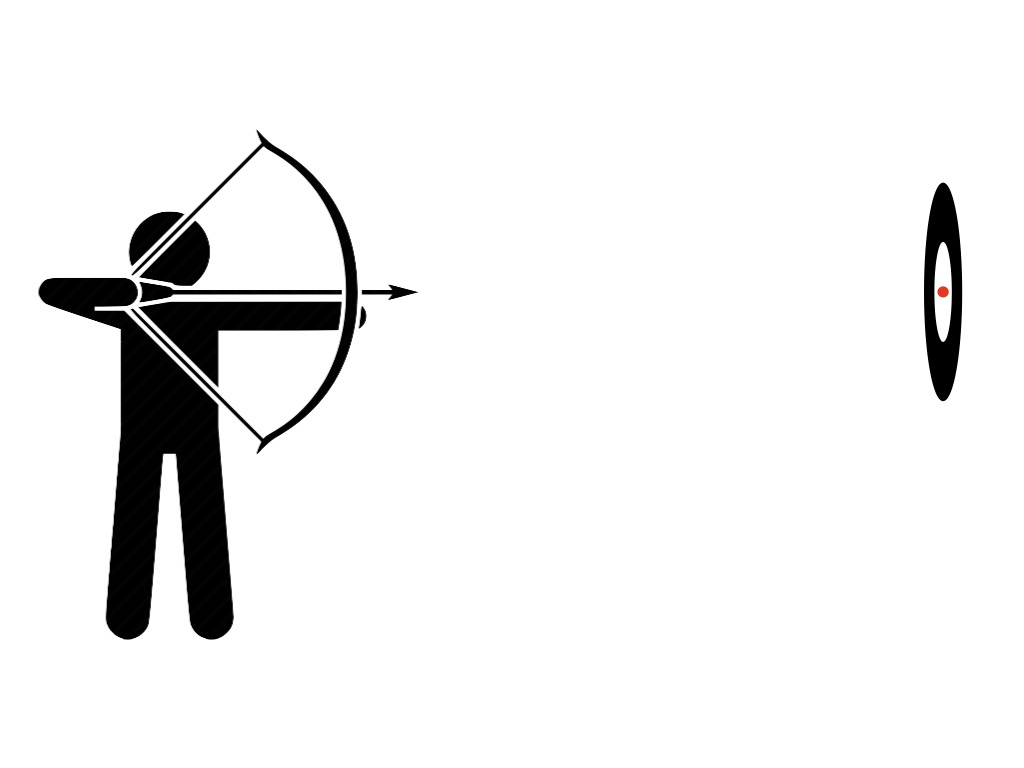
\includegraphics[width=0.5\textwidth]{pictures/archer.png}\end{center}
%---EBLANK #\newpage


%---BBLANK
Continuity of functions of several variables $f\colon \R^{n}\to \R^{m}$ is defined in a similar way. 
Recall that $\R^{n} := \{(x_{1}, \dots, x_{n})  \  |  \  x_{i}\in \R \}$.
If $x=(x_{1}, \dots, x_{n})$ and $y= (y_{1}, \dots, y_{n})$ are two points in $\R^{n}$ then the distance 
between $x$ and $y$ is given by
$$d(x, y) = \sqrt{(x_1-y_1)^2 + \dots + (x_n-y_n)^2}$$  
The number $d(x, y)$ is the length of the straight line segment joining the points $x$ and $y$: 

\begin{equation*}
\begin{tikzpicture}[scale = 1] 
\draw[->, >=latex, thick] (-0.5,0.2) -- (2.5,0.2);
\draw[->, >=latex, thick] (0,-0.3) -- (0 , 2.5) ;
\draw[densely dotted] (-0.5, 0.5) -- (2.5, 2.0);
\fill (0.4, 0.5*0.4+0.75) circle (0.07);
\fill (2.0, 1.75) circle (0.07);
\draw[red, very thick, |-|] (0.39, 0.5*0.39+0.75) -- (2.01, 0.5*2.01+0.75) 
node[midway,sloped,above] {\small \color{red} $d(x, y)$};
\end{tikzpicture}
\end{equation*}
%---EBLANK # \vskip 50mm

%---BBLANK
\begin{definition} 
A function $f\colon \R^n\to \R^m$ is 
\emph{continuous at $x_0\in \R^{n}$} if for each $\varepsilon >0$ there exists 
$\delta >0$ such that if $d(x_0, x)< \delta$ then $d(f(x_0), f(x))< \varepsilon$.

\begin{equation*}
\begin{tikzpicture}[scale = 1] 
\begin{scope}
\draw[->, >=latex, thick] (-0.4,0) -- (2.5,0);
\draw[->, >=latex, thick] (0,-0.4) -- (0 , 2.5) ;
\draw[red, fill = mypink] (1.2,1.2) circle (0.7);
\fill (1.2,1.2) circle (0.07);
\draw[<->, >=latex, red] (0.5, 1.2) -- (1.13 , 1.2) node[midway, above] {\small  $\ \delta$};
\node at (1.25, 0.95) {\small $x_{0}$};
\node at (0.35, 2.35) {\small $\R^{n}$};
\end{scope}

\begin{scope}[xshift = 36mm]
\draw[->, >=latex, thick] (0, 1.2) to[out = 40, in = 140] node[above] {\small $f$} (1.8, 1.2);
\end{scope}

\begin{scope}[xshift = 70mm]
\draw[->, >=latex, thick] (-0.4,0) -- (2.5,0);
\draw[->, >=latex, thick] (0,-0.4) -- (0 , 2.5) ;
\draw[fill = mygray2] (1.2,1.2) circle (1);
\draw[red, fill = mypink, scale = 1.1, yshift = -8.5mm, xshift= -17mm] 
plot [smooth cycle, tension = 0.9] 
coordinates{ (2.2, 2) (2.1, 1.6) (2.5, 1.5) (3, 1.2) (3.3, 1.6) (3.6, 1.8) (3.3, 2.15) (3.1, 2.6) (2.5, 2.35) (2.15, 2.3) };
\fill (1.2,1.2) circle (0.07);
\draw[<->, >=latex] (0.2, 1.2) -- (1.13 , 1.2) node[midway, above] {\small  $\ \varepsilon$};
\node at (1.35, 0.9) {\small $f(x_{0})$};
\node at (0.35, 2.35) {\small $\R^{m}$};
\end{scope}

\end{tikzpicture}
\end{equation*}
\end{definition}
%---EBLANK # \newpage

The above picture motivates the following, more geometric reformulation of continuity:

%---BBLANK
\begin{definition}
\index{ball! open@{open $\sim$}}
Let $x_0\in \R^n$ and let $r>0$. An \emph{open ball}
with radius $r$ and with center at $x_0$ is the set 
$$B(x_0, r) = \{ x\in \R^n \ | \ d(x_0, x) < r\}$$
\begin{equation*}
\begin{tikzpicture}[scale = 1] 
\draw[->, >=latex, thick] (-0.4,0) -- (2.5,0);
\draw[->, >=latex, thick] (0,-0.4) -- (0 , 2.5) ;
\draw[fill = mygray2] (1.2,1.2) circle (1);
\fill (1.2,1.2) circle (0.07);
\draw[<->, >=latex] (0.2, 1.2) -- (1.13 , 1.2) node[midway, above] {\small  $\ r$};
\node at (1.25, 0.95) {\small $x_{0}$};
\node at (0.35, 2.35) {\small $\R^{n}$};
\end{tikzpicture}
\end{equation*}
\end{definition}
%---EBLANK # \vskip 20mm

%---BBLANK
Using this terminology we can say that a function $f\colon \R^{n}\to \R^{m}$ is continuous at $x_{0}$ if for each 
$\varepsilon>0$ there is a $\delta>0$ such $f(B(x_{0}, \delta))\subseteq B(f(x_{0}), \varepsilon)$:
\begin{equation*}
\begin{tikzpicture}[scale = 1] 

\fill[opacity = 0] (-1.5, 0) circle (0.07); % for centering

\begin{scope}
\draw[->, >=latex, thick] (-0.4,0) -- (2.5,0);
\draw[->, >=latex, thick] (0,-0.4) -- (0 , 2.5) ;
\draw[red, fill = mypink] (1.2,1.2) circle (0.7);
\fill (1.2,1.2) circle (0.07);
\draw[<->, >=latex, red] (0.5, 1.2) -- (1.13 , 1.2) node[midway, above] {\small  $\ \delta$};
\node at (1.25, 0.95) {\small $x_{0}$};
\node at (0.35, 2.35) {\small $\R^{n}$};
\node[anchor= south west] at (1.3, 1.75) {\color{red} \small $B(x_{0}, \delta)$};
\end{scope}

\begin{scope}[xshift = 36mm]
\draw[->, >=latex, thick] (0, 1.2) to[out = 40, in = 140] node[above] {\small $f$} (1.8, 1.2);
\end{scope}

\begin{scope}[xshift = 70mm]
\draw[->, >=latex, thick] (-0.4,0) -- (2.5,0);
\draw[->, >=latex, thick] (0,-0.4) -- (0 , 2.5) ;
\draw[fill = mygray2] (1.2,1.2) circle (1);
\draw[red, fill = mypink, scale = 1.1, yshift = -8.5mm, xshift= -17mm] 
plot [smooth cycle, tension = 0.9] 
coordinates{ (2.2, 2) (2.1, 1.6) (2.5, 1.5) (3, 1.2) (3.3, 1.6) (3.6, 1.8) (3.3, 2.15) (3.1, 2.6) (2.5, 2.35) (2.15, 2.3) };
\fill (1.2,1.2) circle (0.07);
\draw[<->, >=latex] (0.2, 1.2) -- (1.13 , 1.2) node[midway, above] {\small  $\ \varepsilon$};
\node at (1.35, 0.9) {\small $f(x_{0})$};
\node at (0.35, 2.35) {\small $\R^{m}$};
\node[anchor= south west] at (1.85, 1.75) {\small $B(f(x_{0}), \varepsilon)$};
\draw[->, >= latex,    thick, red] (0.9, -0.35) .. controls +(-0.3, 0) and +(-0.4, -0.8)..(0.8, 0.738); 
\node[anchor = west] at (0.8, -0.4) {\small \color{red} $f(B(x_{0}, \delta))$};
\end{scope}

\end{tikzpicture}
\end{equation*}
%---EBLANK # \vskip 20mm

%---BBLANK
Here is one more way of rephrasing the definition of continuity: $f\colon \R^{n}\to \R^{m}$
is continuous at $x_{0}$ if for each $\varepsilon >0$ there exists $\delta >0$ such that 
$B(x_{0}, \delta) \subseteq f^{-1}(B(f(x_{0}), \varepsilon))$:
\begin{equation*}
\begin{tikzpicture}[scale = 1] 

\fill[opacity = 0] (-1.5, 0) circle (0.07); % for centering

\begin{scope}
\draw[fill = mygray2, scale = 1] 
plot [smooth cycle, tension = 0.85] coordinates{(0.55, 2.0) (0.65, 0.55)  (2.25, 0.47) (2.5, 2.4)};
\draw[->, >= latex,    thick] (0.9, -0.35) .. controls +(0, 0) and +(-0.4, -0.8)..(0.8, 0.43); 
\node[anchor = west] at (0.8, -0.4) {\small $f^{-1}(B(f(x_{0}), \varepsilon))$};
\draw[->, >=latex, thick] (-0.4,0) -- (2.5,0);
\draw[->, >=latex, thick] (0,-0.4) -- (0 , 2.5) ;
\draw[red, fill = mypink] (1.2,1.2) circle (0.7);
\fill (1.2,1.2) circle (0.07);
\draw[<->, >=latex, red] (0.5, 1.2) -- (1.13 , 1.2) node[midway, above] {\small  $\ \delta$};
\node at (1.25, 0.95) {\small $x_{0}$};
\node at (0.35, 2.35) {\small $\R^{n}$};
\node[anchor= south west] at (1.3, 1.75) {\color{red} \small $B(x_{0}, \delta)$};

\end{scope}

\begin{scope}[xshift = 36mm]
\draw[->, >=latex, thick] (0, 1.2) to[out = 40, in = 140] node[above] {\small $f$} (1.8, 1.2);
\end{scope}

\begin{scope}[xshift = 70mm]
\draw[->, >=latex, thick] (-0.4,0) -- (2.5,0);
\draw[->, >=latex, thick] (0,-0.4) -- (0 , 2.5) ;
\draw[fill = mygray2] (1.2,1.2) circle (1);
\fill (1.2,1.2) circle (0.07);
\draw[<->, >=latex] (0.2, 1.2) -- (1.13 , 1.2) node[midway, above] {\small  $\ \varepsilon$};
\node at (1.35, 0.9) {\small $f(x_{0})$};
\node at (0.35, 2.35) {\small $\R^{m}$};
\node[anchor= south west] at (1.85, 1.75) {\small $B(f(x_{0}), \varepsilon)$};
\end{scope}

\end{tikzpicture}
\end{equation*}
%---EBLANK # \newpage



Notice that in order to define continuity of functions $ \R^{n} \to \R^{m}$ we  used only the 
fact the for any two points in $\R^{n}$ or $\R^{m}$ we can compute the distance between these 
points. This suggests that we could define similarly what is means that a function $f\colon X\to Y$
is continuous where $X$ and $Y$ are any sets, provided that we have some way of measuring 
distances between points in these sets. This observation leads to the notion of a metric space:


%---BBLANK
\begin{definition}
\label{METRIC SPACE DEF}
\index{metric space}
\index{metric}
\index{space! metric@{metric $\sim$}}
A \emph{metric space} is a pair $(X, \varrho)$ where $X$ is a set and $\varrho$ is a function 
$$\varrho\colon X\times X \to \R$$
that satisfies the following conditions:
\begin{enumerate}
\item  $\varrho(x, y) \geq 0$ and $\varrho(x, y) = 0$ if and only if $x=y$;
\item  $\varrho(x, y) = \varrho(y,x)$;
\item  for any $x, y, z\in X$ we have $\varrho(x, z) \leq  \varrho(x,y) + \varrho(y,z)$.
\end{enumerate}
The function $\varrho$ is called a \emph{metric} on the set $X$. For $x, y\in X$ the number 
$\varrho(x, y)$ is called the \emph{distance} between $x$ and $y$. 
\end{definition}
%---EBLANK # \vskip 50mm

The first condition in Definition \ref{METRIC SPACE DEF} says  that distances between points
of $X$ are non-negative, and that the only point located within the distance zero from a point 
$x$ is the point $x$ itself. 
The second condition says that the distance from $x$ to $y$ is 
the same as the distance from $y$ to $x$. The third condition is called the 
\index{triangle inequality}\emph{triangle inequality}. 
It says that the distance between points $x$ and $z$ measured directly will never be bigger than 
the number we obtain by taking the distance from $x$ to some intermediary point $y$ and 
adding it to the distance between $y$ and $z$:
\begin{equation*}
\begin{tikzpicture}[scale = 1] 
\draw[red, very thick] (-1, 0) -- 
node[midway, sloped, below] {$\varrho(x, z)$}  (4, 0) -- 
node[midway, sloped, above] {$\varrho(y, z)$}
(1, 2) -- 
node[midway, sloped, above] {$\varrho(x,  y)$}
cycle;
\fill (-1,0) circle (0.08) node[below left] {\small $x$};
\fill (4,0) circle (0.08) node[below right] {\small $z$};
\fill (1,2) circle (0.08) node[above] {\small $y$};
\end{tikzpicture}
\end{equation*}


We define continuity of functions between metric spaces the same way as for functions 
between $\R^{n}$ and $\R^{m}$:

%---BBLANK
\begin{definition}
\index{function! continuous@{continuous $\sim$}}
Let $(X, \varrho)$  and $(Y, \mu)$ be  metric spaces. A function $f\colon X\to Y$ is \emph{continuous 
at $x_{0}\in X$} if for each $\varepsilon >0$ there exists $\delta >0$ such that  if $\varrho(x_{0}, x ) < \delta$
then $\mu(f(x_{0}), f(x))) < \epsilon$. 

A function $f\colon X\to Y$ is \emph{continuous} if it is continuous at every point $x_{0}\in X$. 
\end{definition}
%---EBLANK # \newpage

We can reformulate this definition in terms of open balls:

%---BBLANK
\begin{definition}
Let $(X, \varrho)$ be a metric space. For $x_0\in X$ and let $r>0$ the \emph{open ball}
with radius $r$ and with center at $x_0$ is the set 
$$B_{\varrho}(x_0, r) = \{ x\in X \ | \ \varrho(x_0, x) < r\}$$
\end{definition}
%---EBLANK # \vskip 40mm

We will  often write $B(x_{0}, r)$ instead of $B_{\varrho}(x_{0}, r)$ when it will be  clear from the context 
which metric is being used.  

%---BBLANK
Notice that a function $f\colon X\to Y$ between metric spaces $(X, \varrho)$  and $(Y, \mu)$ is continuous 
at $x_{0}\in X$ if and only if for each $\varepsilon >0$ there exists $\delta >0$ such that
$B_{\varrho}(x_{0}, \delta)\subseteq f^{-1}(B_{\mu}(f(x_{0}), \varepsilon))$. 
%---EBLANK # \newpage




Here are some examples of metric spaces:


%---BBLANK
\begin{example}
\index{metric!Euclidean@{Euclidean $\sim$}}
Let $X= \R^{n}$. For $x=(x_{1}, \dots, x_{n})$, $y=(y_{1}, \dots, y_{n})$ define:
$$d(x, y) = \sqrt{(x_1-y_1)^2 + \dots + (x_n-y_n)^2}$$ 
The metric $d$ is called the \emph{Euclidean metric} on $\R^{n}$. 
%---EBLANK # \end{example} \newpage

For example, if $x=(1,3)$ and $y = (4,1)$ are points in $\R^{2}$ then 
$$d(x, y) = \sqrt{(1-4)^{2}+(3-1)^{2}} = \sqrt{13}$$
\begin{equation*}
\begin{tikzpicture}[scale = 0.9] 
\draw[->, >=latex, thick] (-0.4,0) -- (4.9,0);
\draw[->, >=latex, thick] (0,-0.4) -- (0 , 3.6);
\draw[red, very thick] (1, 3) --  node[below, sloped, midway] {\small $\sqrt{(1-4)^{2} + (3-1)^{2}}$} (4,1);
\fill (1,3) circle (0.1);
\node at (0.7, 3.4) {\small $(1, 3)$};
\fill (4,1) circle (0.1); 
\node at (4.5, 0.6){\small $(4, 1)$};
\end{tikzpicture}
\end{equation*}

\end{example}

%---BBLANK
\begin{example}
\index{metric! orthogonal@{orthogonal $\sim$}}
Let $X= \R^{n}$. For $x=(x_{1}, \dots, x_{n})$, $y=(y_{1}, \dots, y_{n})$ define:
$$\varrho_{ort}(x, y) = |x_1-y_1| + \dots + |x_n-y_n|$$ 
The metric $\varrho_{ort}$ is called the \emph{orthogonal metric} on $\R^{n}$. 
%---EBLANK # \end{example} \newpage

For example, if $x=(1,3)$ and $y = (4,1)$ are points in $\R^{2}$ then 
$$\varrho_{ort}(x, y) = |1-4|+|3-1| = 5$$
\begin{equation*}
\begin{tikzpicture}[scale = 0.9] 
\draw[->, >=latex, thick] (-0.4,0) -- (4.9,0);
\draw[->, >=latex, thick] (0,-0.4) -- (0 , 3.6);
\draw[red, very thick] (1, 3) --  node[right, midway] {\small $|3-1|$} (1,1) -- node[below, midway] {\small $|4-1|$} (4,1);
\fill (1,3) circle (0.1);
\node at (1.0, 3.4) {\small $(1, 3)$};
\fill (4,1) circle (0.1); 
\node at (4.5, 0.6){\small $(4, 1)$};
\end{tikzpicture}
\end{equation*}
\end{example}

%---BBLANK
\begin{example}
\label{MAX METRIC EXAMPLE}
\index{metric! maximum@{maximum $\sim$}}
Let $X= \R^{n}$. For $x=(x_{1}, \dots, x_{n})$, $y=(y_{1}, \dots, y_{n})$ define:
$$\varrho_{max}(x, y) = \max\{|x_1-y_1|,  \dots,  |x_n-y_n|\}$$ 
The metric $\varrho_{max}$ is called the \emph{maximum metric} on $\R^{n}$. 
%---EBLANK # \end{example} \newpage

For example, if $x=(1,3)$ and $y = (4,1)$ are points in $\R^{2}$ then 
$$\varrho_{max}(x, y) = \max\{|1-4|, |3-1| \} = 3$$
\begin{equation*}
\begin{tikzpicture}[scale = 0.9] 
\draw[->, >=latex, thick] (-0.4,0) -- (4.9,0);
\draw[->, >=latex, thick] (0,-0.4) -- (0 , 3.6);
\draw[mypink, very thick] (1, 3) --  node[right, midway] {\small $|3-1|$} (1,1) -- (4,1);
\draw[red, very thick] (0.976, 1) -- node[below, midway] {\small $|4-1|$} (4,1);
\fill (1,3) circle (0.1);
\node at (1.0, 3.4) {\small $(1, 3)$};
\fill (4,1) circle (0.1); 
\node at (4.5, 0.6){\small $(4, 1)$};
\end{tikzpicture}
\end{equation*}
\end{example}

%---BBLANK
\begin{example}
\index{metric! hub@{hub $\sim$}}
Let $X= \R^{n}$. For $x=(x_{1}, \dots, x_{n})$, $y=(y_{1}, \dots, y_{n})$ define
$\varrho_{h}(x, y)$ as follows. If $x= y$ then $\varrho_{h}(x, y) = 0$. If $x\neq y$ then
$$\varrho_{h}(x, y) = 
\sqrt{x_{1}^{2}+ \dots + x_{n}^{2}} + \sqrt{y_{1}^{2}+ \dots + y_{n}^{2}}
$$ 
The metric $\varrho_{h}$ is called the \emph{hub metric} on $\R^{n}$. 
%---EBLANK # \end{example} \newpage

For example, if $x=(1,3)$ and $y = (4,1)$ are points in $\R^{2}$ then 
$$\varrho_{h}(x, y) = \sqrt{1^{2}+3^{2}} + \sqrt{4^{2}+1^{2}} = \sqrt{10} + \sqrt{17}$$
\begin{equation*}
\begin{tikzpicture}[scale = 0.9] 
\draw[red, very thick] (1, 3) --  
node[below, sloped, midway] {\small $\ \ \ \ \sqrt{1^{2}+ 3^{2}}$} (0.02,0.02) -- 
node[above, sloped, midway] {\small $\sqrt{4^{2} + 1^{2}}$} (4,1);
\draw[->, >=latex, thick] (-0.4,0) -- (4.9,0);
\draw[->, >=latex, thick] (0,-0.4) -- (0 , 3.6);
\fill[red] (0,0) circle (0.1);
\fill (1,3) circle (0.1);
\node at (1.0, 3.4) {\small $(1, 3)$};
\fill (4,1) circle (0.1); 
\node at (4.5, 0.6){\small $(4, 1)$};
\end{tikzpicture}
\end{equation*}

\end{example}



%---BBLANK
\begin{example}
\index{metric! discrete@{discrete $\sim$}}
Let $X$ be any set. Define a metric $\varrho_{disc}$ on $X$ by 
$$
\varrho_{disc}(x, y) = 
\begin{cases}
1 & \text{if } x\neq y \\
0 &  \text{if } x=y \\
\end{cases}
$$
The metric $\varrho_{disc}$ is called the \emph{discrete metric} on $X$. 
%---EBLANK # \end{example} \vskip 80mm
\begin{equation*}
\begin{tikzpicture}[scale=1] 
\draw (0.5, 0) rectangle (6.5, 3.8);
\draw[red, very thick] (1.5, 0.5) -- node[above, midway] {$1$} (5, 0.5);
\draw[red, very thick] (1.5, 0.5) -- node[above, midway, sloped] {$1$} (2.5, 3);
\draw[red, very thick] (1.5, 0.5) -- node[above, midway, sloped] {$1$} (2.5, 3);
\draw[red, very thick] (1.5, 0.5) -- node[above, midway, sloped] {$1$} (4, 2);
\draw[red, very thick] (4, 2) -- node[below, midway, sloped] {$1$} (2.5, 3);
\draw[red, very thick] (4, 2) -- node[below, midway, sloped] {$1$} (5, 0.5);
\draw[red, very thick] (4, 2) -- node[below, midway, sloped] {$1$} (5.5, 3);
\draw[red, very thick] (2.5, 3) -- node[above, midway, sloped] {$1$} (5.5, 3);
\draw[red, very thick] (5, 0.5) -- node[below, midway, sloped] {$1$} (5.5, 3);
\fill (1.5, 0.5) circle (0.1);
\fill (5, 0.5) circle (0.1);
\fill (4, 2) circle (0.1);
\fill (2.5, 3) circle (0.1);
\fill (5.5, 3) circle (0.1);
\node at (1, 3.3) {\small $X$};

\end{tikzpicture}
\end{equation*}


\end{example}

%---BBLANK
\begin{example}
If $(X, \varrho)$ is a metric space and $A\subseteq X$ then $A$ is a metric space with the metric 
induced from $X$. 
\end{example}
%---EBLANK # \newpage

%%%%%%%%%%%%%%%%%%%%%%%%%%%%%%%
%  EXERCISES
%%%%%%%%%%%%%%%%%%%%%%%%%%%%%%%



\exercises

\begin{exercise} 
Verify the $\varrho_{max}$ is a metric on $\R^{n}$.
\end{exercise}



\begin{exercise} 
For points $x= (x_{1}, \dots, x_{n})$, $y=(y_{1}, \dots, y_{n})$ in $\R^{n}$
define 
$$\varrho_{min}(x, y) = \min\{|x_1-y_1|,  \dots,  |x_n-y_n|\}$$
Does this define a metric on $\R^{n}$? Justify your answer.
\end{exercise}





\begin{exercise}
\index{metric! p-adic@{$p$-adic $\sim$}}
Let $\Z$ be a set of all integers, and let $p$ be some fixed prime number. For $m, n\in \Z$
define 
$$\varrho_{p}(m, n) := 
\begin{cases}
0 & \text{if } m=n \\
p^{-k} & \text{if } m-n = p^{k}r \text{ where } r\in \Z, \ p\nmid r \\  
\end{cases}
$$
Verify that $\varrho_{p}$ is a metric on $\Z$. It is called the \emph{$p$-adic metric}.
\end{exercise}




\begin{exercise}
Let $S$ be a set and let $\FF(S)$ denote the set of all non-empty finite subsets of $S$. For $A, B\in \FF(S)$
define
$$\varrho(A, B) = 1 - \frac{|A\cap B|}{|A\cup B|}$$
where $|A|$ denotes the number of elements of the set $A$. Show that $\varrho$ is a metric on $\FF(S)$.
\end{exercise}







\begin{exercise}
Draw the following open  balls in $\R^{2}$ defined by the specified metrics:

\vskip -2mm

a)  $B(x_{0}, 1)$ for  $x_{0} = (0, 0)$ and the orthogonal metric $\varrho_{ort}$. \\
b) $B(x_{0}, 1)$ for  $x_{0} = (0, 0)$ and the maximum metric $\varrho_{max}$. \\
c) $B(x_{0}, 1)$ for  $x_{0} = (0, 0)$ and the hub metric $\varrho_{h}$. \\
d) $B(x_{0}, 6)$ for  $x_{0} = (3, 4)$ and the hub metric $\varrho_{h}$. \\
e) $B(x_{0}, 1)$ for  $x_{0} = (3, 4)$ and the hub metric $\varrho_{h}$. \\
\end{exercise}




\begin{exercise}
\label{BALLINBALL EXERCISE}
Let $(X, \varrho)$ be a metric space,  and let $x_{0}\in X$, Show that if $x\in B(x_{0}, r)$ then 
exists $s>0$ such that $B(x, s)\subseteq B(x_{0}, r)$.
\end{exercise} 




\begin{exercise}
a) Let $(X, \varrho)$ be a metric space and let $B(x, r)$, $B(y, s)$ be open balls in $X$ such that 
$B(y, s) \subseteq B(x, r)$ but $B(y, s) \neq B(x, r)$. Show that $s < 2r$. 


b) Give an example of a metric space $(X, \varrho)$ and open balls $B(x, r)$, $B(y, s)$ in $X$ that 
satisfy the assumptions of part a) and such that $s > r$. 
\end{exercise}





\begin{exercise} 
Let $(X, \varrho_{disc})$ be a discrete metric space and let 
$(Y, \mu)$ be some  metric space. Show that every function $f\colon X\to Y$
is continuous. 
\end{exercise}




\begin{exercise}
Consider  $\R^{2}$ as a metric space with the hub metric $\varrho_{h}$ and
$\R^{1}$ as a metric space with the Euclidean metric $d$. 

a) Show that the function $f\colon \R^{2}\to \R^{1}$ given by 
$$
f(x_{1}, x_{2}) = 
\begin{cases}
0 & \text{if } (x_{1}, x_{2}) = (0, 0) \\
1 & \text{otherwise} \\
\end{cases}
$$
is not continuous. 


b) Show that the function $g\colon \R^{2}\to \R^{1}$ given by 
$$
g(x_{1}, x_{2}) = 
\begin{cases}
0 & \text{if }  x_{1}^{2}+x_{2}^{2} < 1 \\
1 & \text{otherwise} \\
\end{cases}
$$
is continuous. 
\end{exercise}






%%%%%%%%%%%%%%%%%%%%%%%%%%%%%%%
%%%%%%%%%%%%%%%%%%%%%%%%%%%%%%%
%%%
%%%  OPEN SETS 
%%%
%%%%%%%%%%%%%%%%%%%%%%%%%%%%%%%
%%%%%%%%%%%%%%%%%%%%%%%%%%%%%%%

%---BBLANK
\chapter{Open Sets}
%---EBLANK #\newpage

\thispagestyle{firststyle}

We have seen that by equipping sets $X$, $Y$ with metrics we can specify 
what it means that a function $f\colon X\to Y$ is continuous. In general 
continuity of functions depends on the choice of metrics: if we have
two different metrics on $X$ (or on $Y$) then a function $f\colon X\to Y$ that is continuous with respect 
to one of these metrics may  be not continuous with respect to the other. This is however not 
always the case. Our first goal  in this chapter will be to show that  if two metrics on $X$ or $Y$ 
are \emph{equivalent} then functions continuous with respect to one of them are continuous with 
respect to the other and vice versa. 

%---BBLANK
\begin{definition}
\label{EQUIV  METRIC DEF}
\index{metric! equivalence of@{equivalence of $\sim$}}
Let $\varrho_{1}$ and $\varrho_{2}$ be two metrics on the same set $X$. We say that 
the metrics $\varrho_{1}$ and $\varrho_{2}$ are  \emph{equivalent} if for every $x\in X$ 
and for every $r>0$ there exist  $s_{1}, s_{2}>0$ such that 
$B_{\varrho_{1}}(x, s_{1})\subseteq B_{\varrho_{2}}(x, r)$  
and $B_{\varrho_{2}}(x, s_{2})\subseteq B_{\varrho_{1}}(x, r)$.
%---EBLANK #\end{definition}
\begin{equation*}
\begin{tikzpicture}[scale = 0.8] 
\begin{scope}
\draw[fill=mygray2] (0, 2) circle (2);
\draw[red, fill = mypink] (-1, 1) rectangle (1, 3);
\node[anchor=base] at (0,1.3) {\small \color{red} $B_{\varrho_{2}(x, s_{2})}$}; 
\node[anchor=south] at (0,0.03) {\small $B_{\varrho_{1}(x, r)}$}; 
\fill (0, 2) circle [radius = 0.07] node[above, xshift=0.8] {\small $x$};
\end{scope}
\begin{scope}[xshift = 40mm]
\draw[red, fill= mypink] (0,0) rectangle (4,4);
\draw[fill = mygray2] (2, 2) circle (1.2);
\node[anchor=base] at (2,1.3) {\small $B_{\varrho_{1}(x, s_{1})}$}; 
\node[anchor=south] at (2,0.03) {\color{red} \small $B_{\varrho_{2}(x, r)}$}; 
\fill (2, 2) circle [radius = 0.07]  node[above, xshift=0.8] {\small $x$};
\end{scope}
\end{tikzpicture}
\end{equation*}
\end{definition}


%---BBLANK # \vskip 60mm
\begin{proposition}
\label{EQUIV METRIC PROP}
Let $\varrho_{1}$, $\varrho_{2}$ be equivalent metrics on a set $X$, and let $\mu_{1}$, $\mu_{2}$ 
be equivalent metrics on a set $Y$.  A function  $f\colon X\to Y$ is continuous with respect 
to the metrics $\varrho_{1}$  and $\mu_{1}$ if and only if it is continuous with respect to the metrics 
$\varrho_{2}$ and $\mu_{2}$. 
\end{proposition}
%---EBLANK


\begin{proof}
Assume that $f$ is continuous with respect to $\varrho_{1}$ and $\mu_{1}$. We will show 
that it is also continuous with respect to $\varrho_{2}$ and $\mu_{2}$ (the argument in the other direction is the same). 
Let $x\in X$ and let $\varepsilon >0$.  We need to show that there is  $\delta>0$ such that  
$B_{\varrho_{2}}(x, \delta)\subseteq f^{-1}(B_{\mu_{2}}(f(x), \varepsilon)))$. 
Since the metrics $\mu_{1}$ and $\mu_{2}$ are equivalent there exists $\varepsilon_{1} > 0$ such that 
$B_{\mu_{1}}(f(x), \varepsilon_{1})) \subseteq B_{\mu_{2}}(f(x), \varepsilon))$, and so 
$f^{-1}(B_{\mu_{1}}(f(x), \varepsilon_{1}))) \subseteq f^{-1}(B_{\mu_{2}}(f(x), \varepsilon)))$.
 Also, since by assumption $f$ is continuous with respect to  $\varrho_{1}$  and $\mu_{1}$, 
 there is $\delta_{1}$ such that  $B_{\varrho_{1}}(x, \delta_{1})\subseteq f^{-1}(B_{\mu_{1}}(f(x), \varepsilon_{1})))$. 
Finally, using equivalence of metrics $\varrho_{1}$ and $\varrho_{2}$ we obtain that there exists $\delta > 0$
such that $B_{\varrho_{2}}(x, \delta)\subseteq B_{\varrho_{1}}(x, \delta_{1})$.  Combining these inclusions we
get  $B_{\varrho_{2}}(x, \delta) \subseteq f^{-1}(B_{\mu_{2}}(f(x), \varepsilon)))$.
\end{proof}

%---BBLANK # \newpage
\begin{example}
\label{EQUIV METRIC EX}
The Euclidean metric $d$, the orthogonal metric $\varrho_{ort}$ and the 
maximum metric $\varrho_{max}$ are equivalent metrics on $\R^{n}$ (exercise). 

\end{example}
%---EBLANK

%---BBLANK # \vskip 20mm
\begin{example}
\label{NONEQUIV METRIC EX}
The following metrics on $\R^{2}$ are not equivalent to one another:
the Euclidean metric $d$, the hub metric $\varrho_{h}$, and the discrete metric 
$\varrho_{disc}$ (exercise).
\end{example}
%---EBLANK

Every metric defines open balls, but even if metrics are equivalent their open balls may look
very differently (compare e.g. open balls in $\R^{2}$ taken with respect to $d$ and $\varrho_{ort}$). 
It turns out, however, that each metric defines also a collection of so-called \emph{open sets}, and that 
open sets defined by two metrics are the same precisely when these metrics are equivalent.  

%---BBLANK # \newpage
\begin{definition}
\label{OPEN SET DEF}
Let $(X, \varrho)$ be a metric space. A subset $U\subseteq X$ is an \emph{open set} if 
$U$ is a union of (perhaps infinitely many) open balls in $X$:
$U = \bigcup_{i\in I} B(x_{i}, r_{i})$.

\begin{equation*}
\begin{tikzpicture}[scale=1] 
\draw (0.5, 0) rectangle (6.5, 3.8);
\fill[mypink] (4.81, 2.13) circle (1.05);
\fill[mypink]  (3.8, 2.13) circle (0.79);
\fill[mypink]  (3.05, 2.55) circle (0.64);
\fill[mypink]  (2.86, 1.84) circle (0.6);
\fill[mypink]  (2.2, 1.2) circle (0.8);
\fill[mypink]  (2.88, 1.33) circle (0.23);
\fill[mypink]  (3.35, 1.6) circle (0.23);
\fill[mypink]  (3.48, 1.49) circle (0.112);
\fill[mypink]  (4.1, 1.55) circle (0.3);
\fill[mypink]  (4.26, 1.32) circle (0.112);
\fill[mypink]  (2.65, 2.42) circle (0.3);
\fill[mypink]  (3.5, 2.74) circle (0.3);
\fill[mypink]  (4.028, 2.71) circle (0.22);
\fill[mypink] (2.52, 2.22) circle (0.19);
\fill[mypink]  (2.4, 1.745) circle (0.3);

\draw[red] (4.81, 2.13) circle (1.05);
\draw[red] (3.8, 2.13) circle (0.79);
\draw[red] (3.05, 2.55) circle (0.64);
\draw[red] (2.86, 1.84) circle (0.6);
\draw[red] (2.2, 1.2) circle (0.8);
\draw[red] (2.88, 1.33) circle (0.23);
\draw[red] (3.35, 1.6) circle (0.23);
\draw[red] (3.48, 1.49) circle (0.112);
\draw[red] (4.1, 1.55) circle (0.3);
\draw[red] (4.26, 1.32) circle (0.112);
\draw[red] (2.65, 2.42) circle (0.3);
\draw[red] (3.5, 2.74) circle (0.3);
\draw[red] (4.028, 2.71) circle (0.22);
\draw[red] (2.52, 2.22) circle (0.19);
\draw[red] (2.4, 1.745) circle (0.3);

\node at (1, 3.3) {\small $X$};
\node at (5.1, 2.7) {\small \color{red} $U$};

\end{tikzpicture}
\end{equation*}
\end{definition}
%---EBLANK

%---BBLANK # \vskip 20mm
\begin{proposition}
\label{OPEN SET INCL BALL PROP}
Let $(X, \varrho)$ be a metric space and let $U\subseteq X$. The following conditions are equivalent:
\begin{enumerate}
\item The set $U$ is open.
\item For every $x\in U$ there exists $r_{x}>0$ such that $B(x, r_{x})\subseteq U$. 
\end{enumerate}
\end{proposition}

\begin{proof}
Exercise.
\end{proof}
%---EBLANK

%---BBLANK # \newpage
\begin{proposition}
\label{OPEN SET EQUIV METRIC PROP}
\index{metric! equivalence of@{equivalence of $\sim$}}
Let $X$ be a set and let $\varrho_{1}$, $\varrho_{2}$ be two metrics on $X$. The following conditions
are equivalent:
\begin{enumerate}
\item The metrics $\varrho_{1}$ and $\varrho_{2}$ are equivalent.
\item A set $U\subseteq X$ is open with respect to the metric $\varrho_{1}$ if and only if it is open with respect
to the metric $\varrho_{2}$. 
\end{enumerate}
\end{proposition}
%---EBLANK

\begin{proof}
1) $\Ra$ 2) Assume that $\varrho_{1}$ and $\varrho_{2}$ are equivalent  and that 
the set $U$ is open with respect
to $\varrho_{1}$. By Proposition \ref{OPEN SET INCL BALL PROP} this means that for every $x\in U$
there exists  $r_{x}>0$ such that $B_{\varrho_{1}}(x, r_{x}) \subseteq U$. Since the metric 
$\varrho_{1}$ is equivalent to $\varrho_{2}$  we can find $s_{x}>0$ such that 
$B_{\varrho_{2}}(x, s_{x})\subseteq B_{\varrho_{1}}(x, r_{x})$. As a consequence for every $x\in U$
we have $B(x, s_{x}) \subseteq U$.


\begin{equation*}
\begin{tikzpicture}[scale=1]
\draw (-0.4,-0.25) rectangle (6, 3.85);
\draw[fill = mygray1] (2, 1.8+1.8) arc [radius = 1.8, start angle = 90, end angle = 270] 
..controls +(1.3, 0) and +(0, -1).. (5.5, 1.8)  
..controls +(0, 1) and +(1.3, 0).. (2, 1.8+1.8);
\draw[fill= mygray3] (2,1.8) circle (1.55);
\draw[red, fill=mypink] (1.2, 1.0) rectangle (2.8, 2.6);
\fill (2, 1.8) circle [radius = 0.07]  node[above, xshift=0.8] {\small $x$};
\node at (0.1 , 3.3) { \small $X$};
\node at (4.5 , 1.8) { \small $U$};
\node at (2, 1.27) {\color{red} \small $B_{\varrho_{2}}(x, s_{x})$};
\node at (2, 0.65) { \small $B_{\varrho_{1}}(x, r_{x})$};

\end{tikzpicture}
\end{equation*}



Using Proposition  \ref{OPEN SET INCL BALL PROP} again we get that the set $U$ is open 
with respect to $\varrho_{2}$. By the same argument we obtain that if $U$ is open with respect to 
$\varrho_{2}$ then it is open with respect to $\varrho_{1}$.



2) $\Ra$ 1)  Exercise.

\end{proof}


Here are some basic properties of open sets in metric spaces:

%---BBLANK # \vskip 110mm
\begin{proposition}
\label{OPEN SET PROP}
Let $(X, \varrho)$ be a metric space. 
\begin{enumerate}
\item The sets $X$ and $\varnothing$ are open sets. 
\item If $U_{i}$ is an open set  for $i\in I$ then the set $\bigcup_{i\in I} U_{i}$ is open. 
\item If $U_{1}$,  $U_{2}$ are open sets then the set $U_{1}\cap U_{2}$  is open.
\end{enumerate}
\end{proposition}


\begin{proof}
Exercise.
\end{proof}
%---EBLANK 

\begin{note}
From part 3) of Proposition \ref{OPEN SET PROP} is follows that if $\{U_{1}, \dots, U_{n}\}$ is a 
finite family of open sets then $U_{1}\cap \dots \cap U_{n}$ is open. However, if
$\{U_{i}\}_{i\in I}$ is an infinite family of open sets then in general the set $\bigcap_{i\in I} U_{i}$ 
need not be open (exercise).   
\end{note}



Our original definition of a continuous function between metric spaces stated  that 
continuous functions behave well with respect to open balls.
The next proposition says that in order to check if a function is continuous it is enough to 
know how it behaves with respect to open sets:

%---BBLANK # \newpage
\begin{proposition}
\label{CONT FUNCT VIA OPEN SETS PROP}
Let $(X, \varrho)$, $(Y, \mu)$ be metric spaces and let $f\colon X \to Y$ be a function. 
The following conditions are equivalent:
\begin{enumerate}
\item The function $f$ is continuous. 
\item For every open set $U\subseteq Y$ the set $f^{-1}(U)$ is open in $X$.  
\end{enumerate}
\end{proposition}
%---EBLANK 

The proof of Proposition \ref{CONT FUNCT VIA OPEN SETS PROP} will use the following fact:

%---BBLANK # \vskip 20mm
\begin{lemma}
\label{INV IMG OPEN BALL LEMMA}
Let $(X, \varrho)$, $(Y, \mu)$ be metric spaces and let $f\colon X\to Y$ be a continuous function. 
If $B:= B(y_{0}, r)$ is an open ball in $Y$ then the set $f^{-1}(B)$ is open in $X$. 
\end{lemma}

\begin{proof}
Exercise.
\end{proof}
%---EBLANK 


\begin{proof}[Proof of Proposition \ref{CONT FUNCT VIA OPEN SETS PROP}]
1) $\Ra$ 2) Assume that $f\colon X\to Y$ is a continuous function and that $U\subseteq Y$
is an open set. By definition this means that $U$ is a union of some collection of open balls in $Y$:
$$U = \bigcup_{i\in I} B_{\mu}(y_{i}, r_{i})$$
This gives:
$$f^{-1}(U) = f^{-1}\left(\bigcup_{i\in I} B_{\mu}(y_{i}, r_{i})\right) = \bigcup_{i\in I} f^{-1}(B_{\mu}(y_{i}, r_{i}))$$
Since by Lemma \ref{INV IMG OPEN BALL LEMMA} each of the sets $f^{-1}(B_{\mu}(y_{i}, r_{i})$ is open in 
$X$ and  by  Proposition \ref{OPEN SET PROP} a union of open sets is open we obtain that the set 
$f^{-1}(U)$ is open in $X$.   

2) $\Ra$ 1) Assume that $f^{-1}(U)$ is open in $X$ for  every open set $U\subseteq Y$. 
Given  $x\in X$ and $\varepsilon >0$ take $U = B_{\mu}(f(x), \varepsilon)$. 
By assumption the set  $f^{-1}(B_{\mu}(f(x), \varepsilon))\subseteq X$ is open. Since 
$x\in f^{-1}(B_{\mu}(f(x), \varepsilon))$ this implies that there exists $\delta > 0$
such that $B_{\varrho}(x, \delta) \subseteq  f^{-1}(B_{\mu}(f(x), \varepsilon))$. This shows that  
$f$ is a continuous function. 
\end{proof}


Recall that we introduced metric spaces in order to be able to define continuity of functions. 
Proposition \ref{CONT FUNCT VIA OPEN SETS PROP} says however that to define continuity 
we don't really need to use metrics, it is enough to know which sets are open. 
This observation leads to the following generalization of the notion of a metric space:


%---BBLANK # \newpage
\begin{definition}
\label{TOPOLOGY DEF}
\index{topology}
\index{space! topological@{topological $\sim$}}
\index{set! open@{open $\sim$}}
Let $X$ be a set. A \emph{topology} on $X$ is a collection $\TT$ of subsets of $X$
satisfying the following conditions:
\begin{enumerate}
\item $X, \varnothing\in \TT$;
\item If $U_{i}\in \TT$ for $i\in I$ then $\bigcup_{i\in I} U_{i}\in \TT$; 
\item If $U_{1}, U_{2}\in \TT$ then $U_{1}\cap U_{2}\in \TT$.
\end{enumerate}
Elements of $\TT$ are called \emph{open sets}.

A \emph{topological space} is a pair $(X, \TT)$ where $X$ is a set and $\TT$ is a topology on 
$X$. 
\end{definition}
%---EBLANK 

In the setting of topological spaces we can define continuous functions as follows:

%---BBLANK # \vskip 10mm
\begin{definition}
\index{function! continuous@{continuous $\sim$}}
Let $(X, \TT_{X})$, $(Y, \TT_{Y})$ be topological spaces. A function $f\colon X\to Y$ is 
\emph{continuous} if for every $U\in \TT_{Y}$ we have $f^{-1}(U)\in \TT_{X}$. 
\end{definition}
%---EBLANK 

%---BBLANK # \vskip 10mm
\begin{example}
\label{METRIC TOP EXAMPLE}
\index{topology!induced by a metric@{$\sim$ induced by a metric}}
If $(X, \varrho)$ is a metric space then $X$ is a topological space with the topology 
$$\TT= \{U\subseteq X \ | \ U \text{ is a union of open balls}\}$$
We say that the topology $\TT$ is \emph{induced by the metric $\varrho$}.
\end{example}
%---EBLANK 

\begin{note}
From now on, unless indicated otherwise, we will consider $\R^{n}$ as a topological space with 
the topology induced by the Euclidean metric. 
\end{note}

%---BBLANK # \vskip 10mm
\begin{example}
\index{topology! discrete@{discrete $\sim$}}
Let $X$ be an arbitrary set and let 
$$\TT= \{ \text{all subsets of $X$}\}$$
The topology $\TT$ is called the \emph{discrete topology} on $X$. If $X$ is equipped with this topology 
then we say that it is a \emph{discrete topological space}. 
%---EBLANK # \end{example} 


Note that the discrete topology is induced by the discrete metric $\varrho_{disc}$ on $X$. 
Indeed, for $x\in X$ we have 
$$B_{\varrho_{disc}}\left(x, \tfrac{1}{2}\right) = \{x\}$$
so for any subset $U\subseteq X$ we get 
$$U = \bigcup_{x\in U}B_{\varrho_{disc}}\left(x, \tfrac{1}{2}\right) $$
\end{example}


%---BBLANK # \vskip 10mm
\begin{example}
\label{ANTIDISCRT TOP EXAMPLE}
\index{topology! antidiscrete@{antidiscrete $\sim$}}
Let $X$ be an arbitrary set and let 
$$\TT = \{X, \varnothing\}$$
The topology $\TT$ is called the \emph{antidiscrete topology} on $X$. 
\end{example}
%---EBLANK


%---BBLANK # \vskip 10mm
\begin{example}
\index{topology! Zariski@{Zariski $\sim$}}
Let $X= \R$ and let 
$$\TT = \{U\subseteq \R \ | \ U= \varnothing \text{ or $U= (\R\ssmin S)$ for some finite set $S\subseteq \R$}\}$$
The topology $\TT$ is called the \emph{Zariski topology} on $\R$. 
\end{example}
%---EBLANK

One can ask whether for every topological space $(X, \TT)$ we can find a metric $\varrho$ on $X$
such that the topology $\TT$ is induced by $\varrho$. Our next goal is to show 
that this is not the case: some topologies  do not come from any metric. Thus, the notion of a topological 
space is more general than that of a metric space.  

%---BBLANK # \newpage
\begin{definition}
\index{space! metrizable@{metrizable $\sim$}}
A topological space $(X, \TT)$ is \emph{metrizable} if there exists a metric $\varrho$ on $X$
such that $\TT$ is the topology induced by $\varrho$. 
\end{definition}
%---EBLANK

%---BBLANK # \vskip 80mm
\begin{lemma}
\label{METRIC SP IS T1 LEMMA}
If $(X, \TT)$ is a metrizable topological space and $x, y\in X$ are points such that $x\neq y$
then there exists an open set $U\subseteq X$ such that $x\in U$ and $y\not\in U$.
\end{lemma}

\begin{proof}
Exercise. 
\end{proof}
%---EBLANK

%---BBLANK # \vskip 20mm
\begin{proposition}
If $X$ is a set containing more than one point then the antidiscrete topology on $X$  
is not metrizable.  
\end{proposition}
%---EBLANK

\begin{proof}
This follows directly from Lemma \ref{METRIC SP IS T1 LEMMA}. 
\end{proof}

%%%%%%%%%%%%%%%%%%%%%%%%%%%%%%%
%  EXERCISES
%%%%%%%%%%%%%%%%%%%%%%%%%%%%%%%

\exercises


\begin{exercise}
Verify the statement of Example \ref{EQUIV METRIC EX}.
\end{exercise}



\begin{exercise}
Verify the statement of Example \ref{NONEQUIV METRIC EX}.
\end{exercise}




\begin{exercise}
The goal of this exercise is to show that the converse of Proposition \ref{EQUIV METRIC PROP}
is also true. Let $X$ be a set and let $\varrho_{1}, \varrho_{2}$ be two metrics on $X$. 

a)  Assume that for each metric space $(Y, \mu)$ and for each function $f\colon X \to Y$ the function 
$f$  is continuous with respect to $\varrho_{1}$ and $\mu$ if and only if it is continuous respect to $\varrho_{2}$ and $\mu$. 
Show that $\varrho_{1}$ and $\varrho_{2}$ must be equivalent metrics. 

b) Assume that for each metric space $(Y, \mu)$ and for each function $g\colon Y \to X$ the function 
$g$  is continuous with respect to  $\mu$ and $\varrho_{1}$  if and only if it is continuous respect to  $\mu$ and $\varrho_{2}$. 
Show that $\varrho_{1}$ and $\varrho_{2}$ must be equivalent metrics. 
\end{exercise}




\begin{exercise} 
Prove Proposition \ref{OPEN SET INCL BALL PROP}.
\end{exercise}




\begin{exercise}
Consider the set $\R^{2}$ with the Euclidean metric. 

a)  Show that the open half plane $H = \{(x_{1}, x_{2})\in \R^{2} \ | \ x_{2}>0\}$
is an open set in $\R^{2}$

b)  Show that the closed half plane
$\xov{H} = \{(x_{1}, x_{2})\in \R^{2} \ | \ x_{2}\geq 0\}$
is not an open set in $\R^{2}$
\end{exercise}





\begin{exercise}
Consider the set $\R^{2}$ with the hub metric $\varrho_{h}$. Show that the set 
$$A = \{(x_{1}, x_{2})\in \R^{2} \ | \ x_{2}\geq -1\}$$
is an open set in $\R^{2}$
\end{exercise}




\begin{exercise} 
Consider the set $\R$ with the Euclidean metric. Show that every open set in $\R$
is a \emph{disjoint} union of open intervals $(a, b)$ (where possibly $a=-\infty$
or $b= +\infty$).
\end{exercise}



\begin{exercise} 
Prove the implication 2) $\Ra$ 1) of Proposition \ref{OPEN SET EQUIV METRIC PROP}.
\end{exercise}






\begin{exercise} 
Prove Proposition \ref{OPEN SET PROP}.
\end{exercise}





\begin{exercise} 
Consider the set $\R^{2}$ with the Euclidean metric. Give an example of open sets 
$U_{1}, U_{2}, \dots, $ in $\R^{2}$ such that the set $\bigcap_{n=1}^{\infty} U_{i}$ is not open.
\end{exercise}




\begin{exercise} 
Prove Lemma \ref{INV IMG OPEN BALL LEMMA}.
\end{exercise}




\begin{exercise} 
Prove Lemma \ref{METRIC SP IS T1 LEMMA}. 
\end{exercise}




\begin{exercise} 
\label{ZARISKI NOT METRIZABLE EXERCISE}
Show that the set $\R$ with the Zariski topology is not metrizable. 
\end{exercise}




\begin{exercise}
Let $X$ be a topological space consisting of a finite number of points. Show that if $X$ is metrizable then
it is a discrete space. 
\end{exercise}





\begin{exercise}
Let $\R_{Eu}$ denote the set $\R$ with the Euclidean topology and $\R_{Za}$ 
the set $\R$ with the Zariski topology. Show that every continuous function 
$f\colon \R_{Za} \to \R_{Eu}$  must be constant. 
\end{exercise}












%%%%%%%%%%%%%%%%%%%%%%%%%%%%%%%
%%%%%%%%%%%%%%%%%%%%%%%%%%%%%%%
%%%
%%%  BASIS, SUBBASIS, SUBSPACE 
%%%
%%%%%%%%%%%%%%%%%%%%%%%%%%%%%%%
%%%%%%%%%%%%%%%%%%%%%%%%%%%%%%%

%---BBLANK
\chapter[Basis, Subbasis, Subspace]{Basis, Subbasis, \\ Subspace}
%---EBLANK

\thispagestyle{firststyle}


Our main goal in this chapter is to develop some tools that make it easier to construct 
examples of topological spaces. By Definition \ref{TOPOLOGY DEF}
in order to define a topology on a set  $X$ we need to specify which subsets of $X$ 
are open sets. It   can difficult to describe all open sets explicitly,  so topological spaces 
are often  defined by giving either a \emph{basis} or a \emph{subbasis} of a  topology. 
Interesting topological spaces can be also obtained by considering \emph{subspaces}
of  topological spaces. We explain  these notions below. 

%---BBLANK
\begin{definition}
\label{TOP BASIS DEF}
\index{basis of topology}
Let $X$ be a set and let $\mathcal{B}$ be a collection of subsets of $X$. 
The collection $\mathcal{B}$ is a  \emph{basis} on $X$ if it satisfies
the following conditions:
\benu
\item $X = \bigcup_{V\in \BB} V$;
\item for any $V_{1}, V_{2}\in \BB$ and $x\in V_{1}\cap V_{2}$ there exists $W\in \BB$
such that $x\in W$ and $W\subseteq V_{1}\cap V_{2}$. 
\eenu

\begin{equation*}
\begin{tikzpicture}[scale=0.8]
\draw (-0.4, 0) rectangle (5.5, 3.8);
\draw[fill = mygray2, opacity = 0.7, scale = 1.4, yshift = -5mm, xshift= -4mm] 
plot [smooth cycle, tension = 0.8] coordinates{(1, 1.5) (2.3, 1.0) (3, 2.2) (2, 2.8) (1, 2.7) };
\draw[draw= black, fill = mygray2, opacity = 0.7, scale = 1.4, yshift = -7mm, xshift=-6mm] 
plot [smooth cycle, tension = 0.8] coordinates{(2, 1.5) (3, 1.0) (4, 2.0) (3, 3) (2, 2.5) };
\draw[scale = 1.4, yshift = -5mm, xshift= -4mm] 
plot [smooth cycle, tension = 0.8] coordinates{(1, 1.5) (2.3, 1.0) (3, 2.2) (2, 2.8) (1, 2.7) };
\draw[scale = 1.4, yshift = -7mm, xshift=-6mm] 
plot [smooth cycle, tension = 0.8] coordinates{(2, 1.5) (3, 1.0) (4, 2.0) (3, 3) (2, 2.5) };
\draw[draw = red, fill = mypink] (2.63,1.9) circle [x radius = 0.55, y radius = 0.9, rotate= -20];
\fill (2.65,1.8) circle (0.07);
\node at (2.64, 1.55) {\small $x$};
\node at (2.7, 2.3) {\color{red} \small $W$};
\node at (1.05 , 2.3) { \small $V_{1}$};
\node at (4, 2.3) { \small $V_{2}$};
\node at (0.1, 3.3) { \small $X$};
\end{tikzpicture}
\end{equation*}

\end{definition}
%---EBLANK

%---BBLANK # \vskip 10mm
\begin{example}
If $(X, \varrho)$ is a metric space then the set 
$\BB = \{ B(x, r) \ | \ x\in X, \ r>0\}$
consisting of all open balls in $X$ is a basis on $X$ (exercise).
\end{example}
%---EBLANK


%---BBLANK # \newpage
\begin{proposition}
\label{TOP BASIS PROP}
Let $X$ be a set, and  let  $\BB$ be  a basis on $X$. Let $\TT$ 
denote  the collection of all subsets $U\subseteq X$ that can be obtained as the union of some 
elements of $\BB$:
$U= \bigcup_{V\in \BB_{1}}V$
for some $\BB_{1}\subseteq \BB$. Then $\TT$ is a topology on $X$. 
\end{proposition}

\begin{proof}
Exercise. 
\end{proof}
%---EBLANK


%---BBLANK # \vskip 30mm
\begin{definition}
\index{topology! basis of@{basis of $\sim$}}
Let $\BB$ be a basis on a set $X$ and let $\TT$ be the topology defined as in 
Proposition \ref{TOP BASIS PROP}. In such case we will say that $\BB$ is a \emph{basis 
of the topology} $\TT$ and that $\TT$ is the \emph{topology defined by the basis} $\BB$.  
\end{definition}
%---EBLANK


\begin{example}
Let $(X, \varrho)$ be a metric space, let $\TT$ be the topology on $X$ induced by 
$\varrho$, and let $\BB$ be the collection of all open balls in $X$. Directly from the definition of 
the topology $\TT$ (\ref{METRIC TOP EXAMPLE}) it follows that $\BB$  is a basis 
of $\TT$.   
\end{example}

%---BBLANK # \vskip 30mm
\begin{example}
\label{COUNTABLE RN BASIS EX}
Consider  $\R^{n}$ with the Euclidean metric $d$. Let $\BB$ be the collection of all open 
balls $B(x, r)\subseteq \R^{n}$ such that $r\in \Q$ and $x=(x_{1}, x_{2}, \dots, x_{n})$ where 
$x_{1}, \dots, x_{n}\in \Q$. Then $\BB$ is a basis of the Euclidean topology on $\R^{n}$ (exercise). 

\end{example}
%---EBLANK

\begin{note}
If  a topological space $X$ has a  basis consisting of countably many sets then we say that $X$ satisfies 
the \emph{2 $\!^{\text{nd}}$  countability axiom} or that $X$ is  \emph{second countable}. 
Since the set of rational numbers is countable it follows that the basis of the Euclidean topology 
given in Example \ref{COUNTABLE RN BASIS EX} is countable. Thus, $\R^{n}$ with the Euclidean topology 
is a second countable space. Second countable spaces have some interesting properties, some of which we will 
encounter later on. 
\end{note}


%---BBLANK # \vskip 30mm
\begin{example}
\label{ARROW TOP EXAMPLE}
\index{topology! arrow@{arrow $\sim$}}
The set $\BB = \{ [a, b) \ | \ a, b \in \R \}$ is a basis of a certain topology on $\R$. 
We will call it the \emph{arrow topology}.

\begin{equation*}
\begin{tikzpicture}[xscale= 0.8]
\fill[mypink] (-1, 0.13) --  (1, 0.13)  -- (1.15, 0) -- (1,  -0.13) -- (-1, -0.13) -- cycle;
\fill[mypink] (1, 0.13) -- (1.13, 0) -- (1,  -0.13) -- cycle;
\draw[thick] (-2.5, 0) -- (3.5, 0);
\draw[very thick] (-0.95, -0.15) -- (-1, -0.15) -- (-1, 0.15) -- (-0.95, 0.15);
\draw[very thick] (1, 0.15) -- (1.15, 0) -- (1, -0.15);
\node[anchor = base] at (-1.23, -0.35) {\small $a$}; 
\node[anchor = base] at (1.27, -0.35) {\small $b$}; 
\node[anchor = base] at (3.2, 0.15) {\small $\R$}; 
\end{tikzpicture}
\end{equation*}

\end{example}
%---EBLANK

%---BBLANK # \vfill
\begin{example}
\label{CLOSED INT BASIS EX}
Let $\BB = \{ [a, b] \ | \ a, b \in \R \}$.
The set $\BB$ is a basis of the discrete topology on $\R$ (exercise). 
\end{example}
%---EBLANK

%---BBLANK # \newpage
\begin{example}
Let $X = \{a, b, c, d\}$ and let $\BB = \{\{a, b, c\}, \{b, c, d\}\}$.
The set $\BB$ is not a basis of any topology on $X$ since $b\in \{a, b, c\}\cap \{b, c, d\}$,  and 
$\BB$ does not contain any subset $W$ such that 
$b\in W$ and $ W \subseteq \{a, b, c\}\cap \{b, c, d\}$.
\end{example}
%---EBLANK

%---BBLANK # \vskip 20mm
\begin{proposition}
\label{SUBBASIS PROP}
Let $X$ be a set and let $\SS$ be any collection of subsets of $X$ such that 
$X = \bigcup_{V\in \SS} V$.
Let $\TT$ denote the collection of all subsets of $X$ that can be obtained using two operations:
\benu
\item[1)] taking finite intersections of sets in $\SS$;
\item[2)] taking arbitrary unions of sets obtained in 1).
\eenu  
Then  $\TT$ is a topology on $X$. 
\end{proposition}

\begin{proof}
Exercise. 
\end{proof}
%---EBLANK

%---BBLANK # \vskip 20mm
\begin{definition}
Let $X$ be a set  and let $\SS$ be any collection of subsets of $X$ such that 
$X = \bigcup_{V\in \SS} V$.
The topology $\TT$ defined by Proposition \ref{SUBBASIS PROP} is called 
the \emph{topology generated by $\SS$}, and the collection $\SS$ is called a \emph{subbasis}
of $\TT$.  
\index{subbasis of topology}
\index{topology! subbasis of@{subbasis of $\sim$}}
\end{definition}
%---EBLANK

%---BBLANK # \vskip 20mm
\begin{example}
If $X = \{a, b, c, d\}$ and $\SS = \{\{a, b, c\}, \{b, c, d\}\}$ then the topology generated by $\SS$ is 
$\TT= \{\{a, b, c\}, \{b, c, d\}, \{b. c\}, \{a, b, c, d\}, \varnothing \}$.
\end{example}
%---EBLANK

The notions of a basis and a subbasis provide shortcuts for defining topologies: it is easier to specify 
a basis of a topology than to define explicitly the whole topology (i.e. to describe all open sets). Specifying 
a subbasis is even easier. The price we pay for this convenience is that it is more difficult to identify 
which sets are open if we  know only a basis or a subbasis of a topology: 

%---BBLANK # \newpage
\begin{equation*}
\begin{tikzpicture}
\draw[opacity = 0] (2.5 -7, 0) -- (2.5 + 7, 0); % for centering
\draw (0, 0) rectangle +(5, 2.3) node[align = center, midway] 
{\small topology $\TT$ \\[1.5em] \bf{open sets:} \\ elements of $\TT$}; 

\draw (0, -2.6) rectangle +(5, 2.3) node[align = center, midway] 
{\small basis $\BB$ \\[1.5em] \bf{open sets:} \\ unions of  elements of $\BB$}; 


\draw (0, -5.2) rectangle +(5, 2.3) node[align = center, midway] 
{\small subbasis $\SS$ \\[0.5em] \bf{open sets:} \\ unions of  finite intersections\\  of elements of $\SS$}; 

\draw[->, >=latex, very thick] (-0.5, 2.3) --  node[left, pos=0.95, xshift = -2mm] {\small easier to define} 
(-0.5, -5.2);
\draw[<-, >=latex, very thick] (5.5, 2.3) --  
node[right, align = center, pos=0.07,  xshift = 2mm] {\small easier to identify \\ open sets}
(5.5, -5.2);

\end{tikzpicture}
\end{equation*}
%---EBLANK

The next proposition often simplifies checking if a  function between topological spaces is continuous:

%---BBLANK # \vskip 40mm
\begin{proposition}
\label{BASIS CONT FUNC PROP}
Let $(X, \TT_{X})$, $(Y, \TT_{Y})$ be topological spaces, and let 
$\BB$ be a basis (or a subbasis) of $\TT_{Y}$. 
A function $f\colon X\to Y$ is continuous if and only if $f^{-1}(V)\in \TT_{X}$ for every $V\in \BB$. 
\end{proposition}


\begin{proof}
Exercise.
\end{proof}
%---EBLANK

A useful way of obtaining new examples of topological spaces is by considering subspaces of existing 
spaces: 

%---BBLANK # \newpage
\begin{definition}
\index{subspace}
\index{topology! subspace@{subspace $\sim$}}
Let $(X, \TT)$ be a topological space and let $Y\subseteq X$. The collection
$$\TT_{Y}= \{ Y\cap U \ | \ U\in \TT\}$$
is a topology on Y called the \emph{subspace topology}. We say that $(Y, \TT_{Y})$ is a 
\emph{subspace} of the topological space $(X, \TT)$.  

\begin{equation*}
\begin{tikzpicture}[scale = 0.8] 
\draw[opacity = 0] (-3.9 ,0.1) rectangle (9.8, 0.1);
\draw (0.1,0.1) rectangle (5.8,4.0);
\filldraw[fill = mypink] (4, 2.3) circle [radius = 1.3];
\filldraw[mygray2] (0.5, 0.5) rectangle (4.2, 2.5);

\begin{scope}
\clip (0.5, 0.5) rectangle (4.2, 2.5);
\filldraw[fill = mypink, opacity = 0.4] (4, 2.3) circle [radius = 1.3];
\end{scope}

\draw (0.5, 0.5) rectangle (4.2, 2.5);
\draw[red] (4, 2.3) circle [radius = 1.3];
\node at (0.9, 2.1) {\small $Y$}; 
\node at (0.5, 3.6) {\small $X$}; 
\node at (3.5, 2.1) {\small \color{red} $U\cap Y$}; 
\node at (4.6, 2.95) {\small \color{red} $U$}; 
\draw[->,  >=latex,  thick, red] (6.3, 3.2) .. controls +(-0.5, 0.25) and +(0.5, 0.25)..(4.94, 3.2); 
\node[anchor =  west] at (6.3, 3.1) {\emph{\small \color{red} $U$ is open in $X$}};
\draw[->, >= latex,    thick, red] (2.7, -0.23) .. controls +(-0.8, +0.3) and +(-0.6, -0.8)..(3.3, 1.8); 
\node[anchor = north west] at (2.7, -0.03) {\emph{\small \color{red} $U\cap Y$ is open in $Y$}};
\end{tikzpicture}
\end{equation*}
\end{definition}
%---EBLANK

%---BBLANK # \newpage
\begin{example}
\index{sphere}
\index{Sn@{$S^{n}$}}
\index{circle}
The unit circle $S^{1}$ is defined by
$$S^{1} := \{(x_{1}, x_{2})\in \R^{2} \ | \ x_{1}^{2}+x_{2}^{2} = 1 \}$$
The circle $S^{1}$ is a topological space considered as a subspace of  $\R^{2}$.

\begin{equation*}
\begin{tikzpicture}[scale = 1] 
\draw[opacity = 0] (-5, 0) -- (5, 0);
\draw[->,  >=latex, mygray4, thick] (-2, 0) -- (2,0);
\draw[->,  >=latex, mygray4, thick] (0, -2) -- (0, 2);
\draw[very thick] (0, 0) circle (1.5);
\draw[draw = red, fill=mypink] (1.1, 1.1) circle (0.8);
\begin{scope}
\clip (1.1, 1.1) circle (0.8);
\draw[line width = 2pt, red] (0, 0) circle (1.5);
\end{scope}
\draw[->,  >=latex,  thick, red] (2.5, 1.4)  -- (1.85, 1.4); 
\node[anchor= west] at (2.48, 1.43)  {\small \color{red} \emph{open in $\R^{2}$}}; 
\path[name path = Circle1] (0, 0) circle (1.535) ;
\path[name path = Line1] (1.31, 0)  -- (1.3, 1.5);
\path [name intersections = {of = Circle1 and Line1, by={X}}];
\draw[->,  >=latex,  thick, red]   let \p1 = (X) in  (2.5, \y1) -- (\p1); 
\node[anchor= west] at (2.48, 0.835)  {\small \color{red} \emph{open in $S^{1}$}}; 
\end{tikzpicture}
\end{equation*}

In general the $n$-dimensional sphere $S^{n}$ is defined by
$$S^{n} := \{(x_{1}, \dots, x_{n+1})\in \R^{n+1} \ | \ x_{1}^{2}+\dots + x_{n+1}^{2} = 1 \}$$
It is a topological space considered as a subspace of $\R^{n+1}$. 

\end{example}
%---EBLANK


\begin{example}
\label{Z DISCR SUBSP EX}
Consider $\Z$ as a subspace of $\R$. The subspace topology on $\Z$ is  the same as 
the discrete topology (exercise). 
\end{example}


%---BBLANK # \vskip  30mm
\begin{proposition}
\label{SUBSP CONT FUNCT PROP}
Let $X$ be a topological space and let $Y$ be its subspace. 

1) The inclusion map $j\colon Y \to X$ is a continuous function. \\ 
2)  If $Z$ is a topological space then a function $f\colon Z\to Y$ is continuous if and only if 
the composition $jf\colon Z\to X$ is continuous. 
\end{proposition}


\begin{proof}
Exercise.
\end{proof}
%---EBLANK

%---BBLANK # \vskip 70mm
\begin{proposition}
\label{SUBSPACE BASIS PROP}
Let $X$ be a topological space and let $Y$ be its subspace. If $\BB$ is a 
basis (or a subbasis) of $X$ then the set $\BB_{Y} = \{ U\cap Y \ | \ U\in \BB \}$
is a basis (resp. a subbasis) of $Y$. 
\end{proposition}


\begin{proof}
Exercise.
\end{proof}
%---EBLANK


%%%%%%%%%%%%%%%%%%%%%%%%%%%%%%%
%  EXERCISES
%%%%%%%%%%%%%%%%%%%%%%%%%%%%%%%

\exercises
 
\begin{exercise}
Prove Proposition \ref{TOP BASIS PROP}
\end{exercise}
 
 
 
 

\begin{exercise}
Verify the statement of Example \ref{COUNTABLE RN BASIS EX}.
\end{exercise}
 
 
 
\begin{exercise}
Verify the statement of Example \ref{CLOSED INT BASIS EX}.
\end{exercise}
 
 
 
 \begin{exercise}
Prove Proposition \ref{SUBBASIS PROP}.
\end{exercise}




 \begin{exercise}
Prove Proposition \ref {BASIS CONT FUNC PROP}.
\end{exercise}



 
 \begin{exercise}
Consider the interval $[0, 1]$ as a subspace of $\R$. 
Determine which of the following
sets are open in $[0, 1]$. Justify your answers. 

a) $\left(\tfrac{1}{2}, 1\right)$ \hskip 15mm
b) $\left(\tfrac{1}{2}, 1\right]$ \hskip 15mm
c) $\left(\tfrac{1}{3}, \tfrac{2}{3}\right)$ \hskip 15mm
d) $\left(\tfrac{1}{3}, \tfrac{2}{3}\right]$ \hskip 15mm

\end{exercise}





\begin{exercise}
Verify the statement of Example \ref{Z DISCR SUBSP EX}.
\end{exercise} 




\begin{exercise}
Prove Proposition \ref{SUBSP CONT FUNCT PROP}.
\end{exercise}




\begin{exercise}
The goal of this exercise if to show that the subspace topology is uniquely determined by the properties 
listed in  Proposition \ref{SUBSP CONT FUNCT PROP}. Let $X$ be a topological space, let 
$Y\subseteq X$ and let $j\colon Y \to X$ be the inclusion map. Let  $\TT$ be a topology on $Y$, 
and let $Y_{\TT}$ denote $Y$ considered as a topological space with respect to the topology $\TT$. 
Assume that $Y_{\TT}$  satisfies the following conditions:

1) The map $j\colon Y_{\TT} \to X$ is a continuous function. \\ 
2)  If $Z$ is a topological space then a function $f\colon Z\to Y_{\TT}$ is continuous if and only if 
the composition $jf\colon Z\to X$ is continuous. 

Show that $\TT$ is the subspace topology on $Y$. That is, show that $U\in \TT$ if and only if
$U = Y\cap U'$ where $U'$ is some open set in $X$. 

\end{exercise}




\begin{exercise}
\label{DISCR SECOND CONUNTABLE EXERCISE}
Recall that a topological space $X$ is second countable
if the topology on $X$ has a countable basis.  Show that the discrete topology on a set $X$
is second countable if and only if $X$ is a countable set. 
\end{exercise}




\begin{exercise}
\label{ARROW NOT 2 CONUNTABLE EXERCISE}
\index{topology! arrow@{arrow $\sim$}}
Show that $\R$ with the arrow topology is not second countable. 
(Hint: Assume by contradiction that $\BB= \{ V_{1}, V_{2}, \dots \}$ is a countable basis of the 
arrow topology. Let $\alpha_{i} = \inf V_{i}$.  Take $\alpha_{0}\in \R\ssmin \{\alpha_{1}, \alpha_{2}, \dots \}$. 
Show that the set $[\alpha_{0}, \alpha_{0} + 1)$ is not a union of sets from $\BB$).
\end{exercise}




\begin{exercise}
\index{topology! finer@{finer $\sim$}}
Let $\TT_{1}$ and $\TT_{2}$ be two topologies on the same set $X$. We say that the topology 
$\TT_{2}$ is \emph{finer} than $\TT_{1}$ if $\TT_{1}\subseteq \TT_{2}$ 
(e.i. if every open set in $\TT_{1}$ is also open in $\TT_{2}$). Let $\TT_{Ar}$ be the arrow 
topology on $\R$ and let $\TT_{Eu}$ be the Euclidean topology on $\R$. Show that 
$\TT_{Ar}$ is finer than $\TT_{Eu}$.
\end{exercise}





\newpage
%%%%%%%%%%%%%%%%%%%%%%%%%%%%%%%
%%%%%%%%%%%%%%%%%%%%%%%%%%%%%%%
%%%
%%%  CLOSED SETS, INTERIOR, CLOSURE,
%%%  BOUNDARY
%%%
%%%%%%%%%%%%%%%%%%%%%%%%%%%%%%%
%%%%%%%%%%%%%%%%%%%%%%%%%%%%%%%

%---BBLANK
\chapter[Closed Sets]{Closed Sets, \\ Interior, Closure, \\ Boundary}
%---EBLANK

\thispagestyle{firststyle}

%---BBLANK
\begin{definition}
\label{CLOSED SET DEF}
\index{set! closed@{closed $\sim$}}
Let $X$ be a topological space. A set $A\subseteq X$ is a \emph{closed set} if the 
set $X\ssmin A$ is open.
\end{definition}
%---EBLANK

\begin{example}
A closed interval $[a, b]\subseteq \R$ is a closed set since the set 
$\R\ssmin [a, b] = (-\infty, a)\cup (b, +\infty)$
is open in $\R$.
\end{example}

\begin{example}
Let $\TT_{Za}$ be the Zariski topology on $\R$. Recall that $U\in \TT_{Za}$ if 
either $U = \varnothing$ or $U = \R\ssmin S$ where $S\subset \R$ is a finite set. 
As a consequence closed sets in the Zariski topology are the whole space $\R$ and 
all finite subsets of $\R$.
\end{example}

\begin{example}
If $X$ is a topological space with the discrete topology then every subset $A\subseteq X$
is closed in $X$ since every set $X\ssmin A$ is open in $X$. 
\end{example}


%---BBLANK # \newpage
\begin{proposition}
\label{CLOSED SETS PROP}
Let $X$ be a topological space. 
\benu
\item The sets $X$, $\varnothing$ are closed. 
\item If $A_{i}\subseteq X$ is a closed set for $i\in I$ then $\bigcap_{i\in I} A_{i}$ is closed. 
\item If $A_{1}$, $A_{2}$ are closed sets then the set $A_{1}\cup A_{2}$ is   closed. 
\eenu
\end{proposition}
 %---EBLANK
 
 \begin{proof}
1) The set $X$ is closed since the set $X\ssmin X = \varnothing$ is open. Similarly, the set 
$\varnothing$ is closed since the set $X\ssmin \varnothing = X$ is open. 

2) We need to show that the set $X\ssmin \bigcap_{i\in I} A_{i}$ is open. By De Morgan's Laws
(\ref{SET ALG NN}) we have:
$$X\ssmin \bigcap_{i\in I} A_{i} = \bigcup_{i\in I} (X\ssmin A_{i})$$
By assumption the sets $A_{i}$ are closed, so the sets $X\ssmin A_{i}$ are open. Since any 
union of open sets is open we get that $X\ssmin \bigcap_{i\in I} A_{i}$ is an open set. 

3) Exercise. 
%We need to show that the set $X\ssmin (A_{1}\cup A_{2})$ is open. By De Morgan's Laws
%we have:
%$$X\ssmin (A_{1}\cup A_{2}) = (X\ssmin A_{1})\cap (X\ssmin A_{2})$$
%By assumption the sets $A_{1}, A_{2}$ are closed, so the sets $X\ssmin A_{1}$,   $X\ssmin A_{2}$
%are open. Since  intersection  of two open sets is open we get that $X\ssmin (A_{1}\cup A_{2}) $ 
%is an open set. 
 \end{proof}
 
 \begin{note}
 By induction we obtain that if $\{A_{1}, \dots, A_{n}\}$ is a finite collection of closed sets then the set 
 $A_{1}\cup \dots \cup A_{n}$ is closed.  
 It is not true though that an infinite union of closed sets must be  closed. 
 For example, the sets $A_{n} = [\tfrac{1}{n}, 1]$ are closed in $\R$, but the set 
 $\bigcup_{n=1}^{\infty}A_{n} = (0, 1]$ is not closed. 
 \end{note}
 
 In metric spaces closed sets can be characterized using  the notion of convergence of sequences:

%---BBLANK # \newpage
\begin{definition}
\index{sequence!convergent@{convergent $\sim$}}
 Let $(X, \varrho)$ be a metric space, and let $\{x_{n}\}$ be a sequence of points in $X$. 
 We say that $\{x_{n}\}$ \emph{converges} to a point $y\in X$ if for every $\varepsilon >0$
 there exists $N >0$ such that $\varrho(y, x_{n})< \varepsilon$ for all $n> N$.
 We write: $x_{n} \to y$.
 
 Equivalently: $x_{n} \to y$ if  for every $\varepsilon >0$ there exists $N >0$ 
 such that $x_{n}\in B(y, \varepsilon)$  for all $n> N$.
 
\begin{equation*}
\begin{tikzpicture}[scale = 0.8] 
\draw (-0.5,0) rectangle (6,4);
\draw[draw = black, fill = mygray2] (4, 2) circle [radius = 1.5];
\draw[<->, >= latex, ] (4, 2.07)  --  node[right= -1pt] {\small $\varepsilon$}  (4, 3.5);
\fill (0.3, 2) circle [radius = 0.07];
\node[anchor  = base] at (0.33, 1.65) { \small $x_{1}$};
\fill (1.3, 2) circle [radius = 0.07];
\node[anchor  = base] at (1.33, 1.65) { \small $x_{2}$};
\fill (2.1, 2) circle [radius = 0.07];
\fill (2.75, 2) circle [radius = 0.07];
\fill (3.18, 2) circle [radius = 0.07];
\fill (3.53, 2) circle [radius = 0.07];
\fill (3.8, 2) circle [radius = 0.07];
\fill[red] (4, 2) circle [radius = 0.07];
\node[anchor  = base] at (3.99, 1.65) {\color{red} \small $y$}; 
\node at (0 , 3.5) { \small $X$};
\end{tikzpicture}
\end{equation*}
\end{definition}
%---EBLANK
 
 
 %---BBLANK # \vskip 20mm
 \begin{proposition}
 \label{METRIC CL VIA SEQ PROP}
 Let $(X, \varrho)$ be a metric space and let $A\subseteq X$. The following conditions are 
 equivalent: 
 \benu
 \item The set $A$ is closed in $X$. 
 \item If $\{x_{n}\}\subseteq A$  and $x_{n}\to y$ then  $y\in A$. 
 \eenu
 \end{proposition}
 
 
 \begin{proof}
 Exercise.
 \end{proof}
 %---EBLANK
 
 \begin{example}
 Take $\R$ with the Euclidean metric,  and let $A = (0, 1]$. 
  Let $x_{n} = \tfrac{1}{n}$. Then $\{x_{n}\}\subseteq A$, 
 but $x_{n}\to 0\not\in A$. This shows that  $A$ is not a closed set in $\R$.
 \end{example}
 
 
The notion of convergence of a sequence can be extended from metric spaces to general 
topological spaces by replacing open balls with center at a point $y$ with open neighborhoods 
of $y$:
 
%---BBLANK # \newpage
 \begin{definition}
 \index{neighborhood! open@{open $\sim$}}
 Let $X$ be a topological space and $y\in X$. If $U\subseteq X$ is an open set such that 
 $y\in U$ then we say that $U$ is an \emph{open neighborhood of $y$}. 
 \end{definition}
  %---EBLANK
 
 %---BBLANK # \vskip 30mm
 \begin{definition}
 \label{TOP SP SEQ CONV DEF}
 \index{sequence!convergent@{convergent $\sim$}}
 Let $X$ be a topological space. A sequence $\{x_{n}\}\subseteq X$ \emph{converges}
 to $y\in X$ if for every open neighborhood $U$ of  $y$ there exists 
 $N >0$ such that $x_{n}\in U$ for $n> N$.
 
\begin{equation*}
\begin{tikzpicture}[scale=0.8]
\draw (-0.5,0) rectangle (6,4);
\draw[fill= mygray2, scale = 1.4, yshift = -5.5mm, xshift= -1mm] 
plot [smooth cycle, tension = 0.8] coordinates{(2, 1.5) (3, 1.0) (4, 2.0)  (3, 3) (2, 2.5) };
\fill (0.3, 2) circle [radius = 0.07];
\node[anchor  = base] at (0.33, 1.65) { \small $x_{1}$};
\fill (1.3, 2) circle [radius = 0.07];
\node[anchor  = base] at (1.33, 1.65) { \small $x_{2}$};
\fill (2.1, 2) circle [radius = 0.07];
\fill (2.75, 2) circle [radius = 0.07];
\fill (3.18, 2) circle [radius = 0.07];
\fill (3.53, 2) circle [radius = 0.07];
\fill (3.8, 2) circle [radius = 0.07];
\fill[red] (4, 2) circle [radius = 0.07];
\node[anchor  = base] at (3.99, 1.65) {\color{red} \small $y$};
\node at (0 , 3.5) { \small $X$};
\node at (4.5 , 2.8) { \small $U$};
\end{tikzpicture}
\end{equation*}


 \end{definition}
%---EBLANK

  %---BBLANK # \vskip 30mm
 \begin{note}
 In general topological spaces a sequence may converge to many points at the same time. 
 %---EBLANK # \end{note} 
 For example let $(X, \TT)$ be a  space with the antidiscrete topology $\TT= \{X, \varnothing\}$. 
 Any sequence $\{x_{n}\}\subseteq X$ converges to any point $y\in X$ since the only open 
 neighborhood of $y$ is whole space $X$, and $x_{n}\in X$ for all $n$. The next proposition says 
 that such situation cannot happen in metric spaces:
 \end{note}
 
 
 %---BBLANK # \vskip 30mm
 \begin{proposition}
 \label{METRIC UNIQUE CONV PROP}
 Let $(X, \varrho)$ be a metric space and let $\{x_{n}\}$ be a sequence in $X$. If $x_{n} \to y$
and $x_{n} \to  z$ for some $y, z\in X$ then $y=z$. 
 \end{proposition}
 
 \begin{proof}
 Exercise. 
 \end{proof}
%---EBLANK 
 
  %---BBLANK # \newpage
 \begin{proposition}
 \label{SEQ IN CLOSED SET PROP}
 Let $X$ be a topological space and let $A\subseteq X$ be a closed set.  If $\{x_{n}\}\subseteq A$
and  $x_{n}\to y$ then $y\in A$. 
 \end{proposition}
 
 \begin{proof}
 Exercise.
 \end{proof}
 %---EBLANK 
 

 \begin{note}
 For a general topological space $X$ the converse of Proposition \ref{SEQ IN CLOSED SET PROP} 
 is not true. That is, assume   that $A\subseteq X$ is  a set with the property that if
 $\{x_{n}\}\subseteq A$ and $x_{n}\to y$  then $y\in A$. The next example shows  that this 
 does not  imply  that the set $A$ must be closed in $X$. 
 \end{note}
 
 
 %---BBLANK # \vskip 30mm
 \begin{example}
 \label{SEQ NOT CLOSED EXAMPLE}
 Let $X= \R$ with the following topology:
 $$\TT = \{U\subseteq \R \ | \ U= \varnothing \text{ or $U= (\R\ssmin S)$ for some countable set $S\subseteq \R$}\}$$
 Closed sets in $X$ are  the whole space $\R$ and all countable subsets of $\R$.
If $\{x_{n}\}\subseteq X$ is a sequence  then  $x_{n}\to y$ if and only if there exists 
 $N>0$ such that $x_{n} = y$ for all $n> N$ (exercise). 
 It follows that if $A$ is any (closed or not) subset of $X$,  $\{x_{n}\}\subseteq A$,
 and $x_{n}\to y$ then $y\in A$.
 \end{example} 
 %---EBLANK 

 
 %---BBLANK # \newpage
 \begin{definition}
 \index{Int@{$\Int$}}
 \index{Bd@{$\Bd$}}
 \index{set! interior of@{interior of $\sim$}}
 \index{set! closure of@{closure of $\sim$}}
 \index{set! boundary of@{boundary of $\sim$}}
 \index{interior}
 \index{closure}
 \index{boundary ! of a set@{$\sim$ of a set}}
 Let $X$ be a topological space and let $Y\subseteq X$. 
 \bit
 \setlength\itemsep{0.3em}
 \item The \emph{interior of $Y$} is the set 
 $\Int(Y) := \bigcup \ \{ U \ |\ U\subseteq Y \text{ and $U$ is open in $X$} \}$. 
 \item The \emph{closure of $Y$} is the set 
 $\xov{Y} := \bigcap \ \{ A \ |\  Y\subseteq A \text{ and $A$ is closed in $X$} \}$.
 \item The \emph{boundary of $Y$} is the set 
 $\Bd(Y) := \xov{Y} \cap \xov[.9]{(X\ssmin Y)}$.
 \eit 
 \end{definition}
 %---EBLANK 
 
 
 %---BBLANK # \vskip 10mm
 \begin{example}
 Consider the set $Y = (a, b]$ in $\R$:
 \begin{equation*}
\begin{tikzpicture}[scale=1]
\draw[thick] (-2, 0) -- (2, 0);
\draw[red, line width = 3pt] (-1.1, 0) -- (1.1,0);
\draw[draw = red, fill = white, line width = 1.5] (-1.1, 0) circle [radius = 0.1];
\draw[draw = red, fill = red, line width = 1.5] (1.1, 0) circle [radius = 0.1];
\node[anchor=base] at (0, 0.3) {\color{red} \small $Y$};
\node[anchor = base] at (-1.15, -0.5) {\small $a$}; 
\node[anchor = base] at (1.09, -0.5) {\small $b$}; 
\node[anchor = base] at (1.8, 0.15) {\small $\R$}; 
\end{tikzpicture}
\end{equation*}
We have:
\begin{equation*}
\begin{tikzpicture}[scale=1]
\begin{scope}
\draw[thick] (-2, 0) -- (2, 0);
\draw[red, line width = 3pt] (-1.1, 0) -- (1.1,0);
\draw[draw = red, fill = white, line width = 1.5] (-1.1, 0) circle [radius = 0.1];
\draw[draw = red, fill = white, line width = 1.5] (1.1, 0) circle [radius = 0.1];
\node[anchor = base] at (-1.15, -0.5) {\small $a$}; 
\node[anchor = base] at (1.09, -0.5) {\small $b$}; 
\node[anchor = base] at (1.8, 0.15) {\small $\R$}; 
\node[anchor=base] at (0, 0.3) {\color{red} \small $\Int(Y)$};
\node[anchor=base] at (0,-1.3) {$ \Int(Y) = (a, b)$};
\end{scope}

\begin{scope}[xshift = 5cm]
\draw[thick] (-2, 0) -- (2, 0);
\draw[red, line width = 3pt] (-1.1, 0) -- (1.1,0);
\draw[draw = red, fill = red, line width = 1.5] (-1.1, 0) circle [radius = 0.1];
\draw[draw = red, fill = red, line width = 1.5] (1.1, 0) circle [radius = 0.1];
\node[anchor = base] at (-1.15, -0.5) {\small $a$}; 
\node[anchor = base] at (1.09, -0.5) {\small $b$}; 
\node[anchor = base] at (1.8, 0.15) {\small $\R$}; 
\node[anchor=base] at (0, 0.3) {\color{red} \small $\xov{Y}$};
\node[anchor=base] at (-0.1,-1.3) {$ \xov{Y} = [a, b]$};
\end{scope}

\begin{scope}[xshift = 10cm]
\draw[thick] (-2, 0) -- (2, 0);
\draw[draw = red, fill = red, line width = 1.5] (-1.1, 0) circle [radius = 0.1];
\draw[draw = red, fill = red, line width = 1.5] (1.1, 0) circle [radius = 0.1];
\node[anchor = base] at (-1.15, -0.5) {\small $a$}; 
\node[anchor = base] at (1.09, -0.5) {\small $b$}; 
\node[anchor = base] at (1.8, 0.15) {\small $\R$}; 
\node[anchor=base] at (0, 0.3) {\color{red} \small $\Bd(Y)$};
\node[anchor=base] at (0,-1.3) {$ \Bd(Y) = \{a, b\}$};
\end{scope}
\end{tikzpicture}
\end{equation*}
\end{example}
 %---EBLANK 
 
 %---BBLANK # \vskip 10mm
\begin{example}
Consider the set $Y = \{(x_{1}, x_{2})\in \R^{2} \ | \ a < x_{1} \leq b, \ c\leq  x_{2} < d \}$ in $\R^{2}$:
\begin{equation*}
\begin{tikzpicture}[scale = 1] 
\draw[->, >=latex, thick] (-0.5,0) -- (3.1,0);
\draw[->, >=latex, thick] (0,-0.5) -- (0 , 2.3) ;
\fill[mypink] (0.7, 0.5) rectangle (2.5, 1.7);
\draw[red, line width = 2] (0.7, 0.5) -- (2.5, 0.5) -- (2.5, 1.7);
\draw[line width = 2] (-0.06, 1.7) node[anchor =  east ] {\small $d$} -- (0.06, 1.7) ; 
\draw[line width = 2] (-0.06, 0.5) node[anchor =  east ] {\small $c$} -- (0.06, 0.5) ; 
\draw[line width = 2] (0.7, -0.06) node[anchor = north ] {\small $a$} -- (0.7, 0.06) ; 
\draw[line width = 2] (2.5, -0.06) node[anchor = north ] {\small $b$} -- (2.5, 0.06) ; 
\node[anchor= base west] at (0.7, 1.2) {\small \color{red} $Y$};
\end{tikzpicture}
\end{equation*}
We have: 
\begin{equation*}
\begin{tikzpicture}[scale = 1] 
\begin{scope}
\draw[->, >=latex, thick] (-0.5,0) -- (3.1,0);
\draw[->, >=latex, thick] (0,-0.5) -- (0 , 2.3) ;
\fill[mypink] (0.7, 0.5) rectangle (2.5, 1.7);
\draw[line width = 2] (-0.06, 1.7) node[anchor =  east ] {\small $d$} -- (0.06, 1.7) ; 
\draw[line width = 2] (-0.06, 0.5) node[anchor =  east ] {\small $c$} -- (0.06, 0.5) ; 
\draw[line width = 2] (0.7, -0.06) node[anchor = north ] {\small $a$} -- (0.7, 0.06) ; 
\draw[line width = 2] (2.5, -0.06) node[anchor = north ] {\small $b$} -- (2.5, 0.06) ; 
\node[anchor= base west] at (0.7, 1.2) {\small \color{red} $\Int(Y)$};
\node[anchor=base west] at (-0.7,-1.3) {$\Int(Y) = (a, b)\times (c, d)$};
\end{scope}

\begin{scope}[xshift = 50mm]
\draw[->, >=latex, thick] (-0.5,0) -- (3.1,0);
\draw[->, >=latex, thick] (0,-0.5) -- (0 , 2.3) ;
\fill[mypink] (0.7, 0.5) rectangle (2.5, 1.7);
\draw[red, line width = 2] (0.7, 0.5) rectangle (2.5, 1.7);
\draw[line width = 2] (-0.06, 1.7) node[anchor =  east ] {\small $d$} -- (0.06, 1.7) ; 
\draw[line width = 2] (-0.06, 0.5) node[anchor =  east ] {\small $c$} -- (0.06, 0.5) ; 
\draw[line width = 2] (0.7, -0.06) node[anchor = north ] {\small $a$} -- (0.7, 0.06) ; 
\draw[line width = 2] (2.5, -0.06) node[anchor = north ] {\small $b$} -- (2.5, 0.06) ; 
\node[anchor= base west] at (0.7, 1.2) {\small \color{red} $\xov Y$};
\node[anchor=base west] at (-0.1,-1.3) {$\xov Y = [a, b]\times [c, d]$};
\end{scope}

\begin{scope}[xshift = 100mm]
\draw[->, >=latex, thick] (-0.5,0) -- (3.1,0);
\draw[->, >=latex, thick] (0,-0.5) -- (0 , 2.3) ;
\draw[red, line width = 2] (0.7, 0.5) rectangle (2.5, 1.7);
\draw[red, line width = 2] (0.7, 0.5) -- (2.5, 0.5) -- (2.5, 1.7);
\draw[line width = 2] (-0.06, 1.7) node[anchor =  east ] {\small $d$} -- (0.06, 1.7) ; 
\draw[line width = 2] (-0.06, 0.5) node[anchor =  east ] {\small $c$} -- (0.06, 0.5) ; 
\draw[line width = 2] (0.7, -0.06) node[anchor = north ] {\small $a$} -- (0.7, 0.06) ; 
\draw[line width = 2] (2.5, -0.06) node[anchor = north ] {\small $b$} -- (2.5, 0.06) ; 
\node[anchor= base west] at (0.7, 1.2) {\small \color{red} $\Bd(Y)$}; 
\node[anchor=base west] at (-0.7,-1.3) {$\Bd(Y)  = [a, b]\times \{c, d\} $};
\node[anchor=base west] at (0.5, -1.9) {$\cup \{a, b\}\times [c, d] $};
\end{scope}

\end{tikzpicture}
\end{equation*}

 \end{example}
 %---EBLANK 

 %---BBLANK # \newpage
\begin{proposition}
\label{INT CL PROP}
Let $X$ be a topological space and let $Y\subseteq X$. 
\benu
\item The set $\Int(Y)$ is open in $X$. It is the biggest open set contained in $Y$: if 
$U$ is open and $U\subseteq Y$ then $U\subseteq \Int(Y)$. 
\item The set $\xov{Y}$ is closed in $X$. It is the smallest closed set that contains $Y$: if 
$A$ is closed and $Y\subseteq A$ then $\xov{Y}\subseteq A$. 
\eenu
 
\end{proposition}

\begin{proof}
Exercise.
\end{proof} 
%---EBLANK 

%---BBLANK # \newpage
\begin{proposition}
\label{INT CHARCT PROP}
\index{set! interior of@{interior of $\sim$}}
\index{interior}
Let $X$ be a topological space, let $Y\subseteq X$, and let $x\in X$. The following conditions 
are equivalent:
\benu
\item $x\in \Int(Y)$
\item There exists an open neighborhood $U$ of $x$ such that $U\subseteq Y$. 
\eenu 

\begin{equation*}
\begin{tikzpicture}[scale = 0.8] 
\draw (0,0) rectangle (6,3.5);
\draw[fill = mygray2] (1.5,0.5) rectangle (5.5, 3);
\fill[mypink, opacity = 0.6] (4.3, 1.7) circle [radius = 0.9];
\draw[red] (4.3, 1.7) circle [radius = 0.9];
\fill (4.3, 1.7) circle [radius = 0.07];
\node[anchor  = base] at (3.9, 2.0) {\color{red} \small $U$}; 
\node[anchor  = base] at (4.28, 1.35)  {\small $x$}; 
\node at (0.5 , 3) { \small $X$};
\node at (2 , 2.5) { \small $Y$};
\end{tikzpicture}
\end{equation*}
\end{proposition}
%---EBLANK 

\begin{proof} 
1) $\Ra$ 2)  Assume that $x\in \Int(Y)$. Since $\Int(Y)$ is an open set and $\Int(Y)\subseteq Y$
we can take $U= \Int(Y)$. 


2) $\Ra$ 1)  Assume that $x\in U$ for some open set $U$ such that $U\subseteq Y$. Since $\Int(Y)$
is the union of all open sets contained in $Y$ thus $U\subseteq \Int(Y)$ and so $x\in \Int(Y)$.
\end{proof}
 
%---BBLANK # \newpage
\begin{proposition}
\label{CL CHARCT PROP}
\index{set! closure of@{closure of $\sim$}}
\index{closure}
Let $X$ be a topological space, let $Y\subseteq X$, and let $x\in X$. The following conditions 
are equivalent:
\benu
\item $x\in \xov{Y}$
\item For every open neighborhood $U$ of $x$ we have $U\cap Y \neq \varnothing$. 
\eenu 

\begin{equation*}
\begin{tikzpicture}[scale = 0.8] 
\draw (0,0) rectangle (6,3.5);
\fill[mypink] (1.5, 1.1) circle [radius = 0.9];
\draw[fill = mygray2] (1.5,0.5) rectangle (5.5, 3);
\fill[mypink, opacity = 0.6] (4.3, 1.7) circle [radius = 0.9];
\draw[red] (4.3, 1.7) circle [radius = 0.9];
\fill (4.3, 1.7) circle [radius = 0.07];
\begin{scope}
\clip (1.5,0.5) rectangle (5.5, 3.5);
\fill[mypink, opacity = 0.6] (1.5, 1.1) circle [radius = 0.9];
\end{scope}
\draw (1.5,0.5) rectangle (5.5, 3);
\draw[red] (1.5, 1.1) circle [radius = 0.9];
\node[anchor  = base] at (3.9, 2.0) {\color{red} \small $U_{1}$}; 
\node[anchor  = base] at (4.34, 1.35)  {\small $x_{1}$}; 
\fill (1.5, 1.1) circle [radius = 0.07];
\node[anchor  = base] at (1.1, 1.4) {\color{red} \small $U_{2}$}; 
\node[anchor  = base] at (1.76, 0.8)  {\small $x_{2}$}; 
\node at (0.5 , 3) { \small $X$};
\node at (2 , 2.5) { \small $Y$};
\end{tikzpicture}
\end{equation*}



\end{proposition}
 
\begin{proof}
Exercise.
\end{proof} 
%---EBLANK 

 
%---BBLANK # \vskip 30mm 
\begin{proposition}
\label{BD CHARCT PROP}
\index{set! boundary of@{boundary of $\sim$}}
 \index{boundary ! of a set@{$\sim$ of a set}}
Let $X$ be a topological space, let $Y\subseteq X$, and let $x\in X$. The following conditions 
are equivalent:
\benu
\item $x\in \Bd(Y)$
\item For every open neighborhood $U$ of $x$ we have $U\cap Y \neq \varnothing$ \\
and $U\cap (X\ssmin Y) \neq \varnothing$. 
\eenu 

\begin{equation*}
\begin{tikzpicture}[scale = 0.8] 
\draw (0,0) rectangle (6,3.5);
\fill[mypink] (1.5, 1.1) circle [radius = 0.9];
\draw[fill = mygray2] (1.5,0.5) rectangle (5.5, 3);
\begin{scope}
\clip (1.5,0.5) rectangle (5.5, 3.5);
\fill[mypink, opacity = 0.6] (1.5, 1.1) circle [radius = 0.9];
\end{scope}
\draw (1.5,0.5) rectangle (5.5, 3);
\draw[red] (1.5, 1.1) circle [radius = 0.9];
\fill (1.5, 1.1) circle [radius = 0.07];
\node[anchor  = base] at (1.06, 1.4) {\color{red} \small $U$}; 
\node[anchor  = base] at (1.72, 0.8)  {\small $x$}; 
\node at (0.5 , 3) { \small $X$};
\node at (2 , 2.5) { \small $Y$};
\end{tikzpicture}
\end{equation*}
\end{proposition}
%---EBLANK 

\begin{proof}
This follows from the definition of $\Bd(Y)$ and  Proposition \ref{CL CHARCT PROP}.
\end{proof} 
 

%---BBLANK # \newpage
\begin{definition}
\index{set! dense@{dense $\sim$}}
\index{dense set}
Let $X$ be a topological space. A set $Y\subseteq X$ is \emph{dense in $X$} if $\xov{Y} = X$. 
\end{definition} 
%---EBLANK 

%---BBLANK # \vskip 30mm
\begin{proposition}
\label{DENSE CHARCT PROP}
Let $X$ be a topological space and  let $Y\subseteq X$. The following conditions 
are equivalent:
\benu
\item $Y$ is dense in $X$
\item If $U\subseteq X$ is an open set and $U\neq \varnothing$ then $U\cap Y \neq \varnothing$. 
\eenu 
\end{proposition}
%---EBLANK 

\begin{proof}
This follows directly from Proposition \ref{CL CHARCT PROP}.
\end{proof}
 
%---BBLANK # \vskip 50mm
 \begin{example}
 The set of rational numbers $\Q$ is dense in $\R$. 
 \end{example}
 %---EBLANK 
 
 
%%%%%%%%%%%%%%%%%%%%%%%%%%%%%%%
%  EXERCISES
%%%%%%%%%%%%%%%%%%%%%%%%%%%%%%%

\exercises


\begin{exercise}
Prove Proposition \ref{METRIC CL VIA SEQ PROP}
\end{exercise}



\begin{exercise}
Prove Proposition \ref{METRIC UNIQUE CONV PROP}
\end{exercise}



\begin{exercise}
\index{sequence!Cauchy@{Cauchy $\sim$}}
Let $(X, \varrho)$ be a metric space. A sequence $\{x_{n}\}$ is called a \emph{Cauchy sequence}
if for any $N > 0$ there exists $\varepsilon > 0$ such that if $n, m >  N$ then 
$\varrho(x_{m}, x_{n}) < \varepsilon$. Show that if  $\{x_{n}\}$ is a sequence in $X$ that converges 
to some point $x_{0}\in X$ then $\{x_{n}\}$ is a Cauchy sequence.  
\end{exercise}





\begin{exercise}
Prove Proposition \ref{SEQ IN CLOSED SET PROP}
\end{exercise}



\begin{exercise}
Let $X$ be the topological space defined in Example \ref{SEQ NOT CLOSED EXAMPLE} 
and let  $\{x_{n}\}$ be a sequence in $X$.  Show that  $x_{n}\to y$ for some $y\in X$ iff
there exists $N>0$ such that $x_{n} = y$ for all $n>N$.  
\end{exercise}





 
 \begin{exercise}
Prove Proposition \ref{CL CHARCT PROP}
\end{exercise}
   



\begin{exercise}
\label{CLOSED IN SUBSP EXERCISE}
Let $X$ be a topological space and let $Y$ be a subspace of $X$. 
Show that a set $A\subseteq Y$ is closed in $Y$ if and only if there exists 
a set $B$ closed in $X$ such that $Y\cap B = A$. 
\end{exercise}




\begin{exercise}
Let $X$ be a topological space and let $Y\subseteq X$ be a subspace. For a set 
$A\subseteq Y$  let $\cl_{Y}(A)$ denote the closure of $A$ in $Y$ and $\cl_{X}(A)$
the closure of $A$ taken in $X$. Show that $\cl_{Y}(A) = \cl_{X}(A)\cap Y$.
\end{exercise}



        
\begin{exercise}
\label{OPEN CLOSED SETS IN SUBSP EXERCISE}
Let $X$ be a topological space and let $Y\subseteq X$ be a subspace. 

a) Assume that  $Y$ is open  in $X$. Show that if  $U\subseteq Y$ is open in $Y$
then $U$ is open in $X$. 

b) Assume that  $Y$ is closed in $X$. Show that if  $A\subseteq Y$ is closed in $Y$
then $A$ is closed in $X$. 
\end{exercise}
           





\begin{exercise}
\label{CLOSED BALL EXERCISE}

\index{ball! closed@{closed $\sim$}}
Let $(X, \varrho)$ be a metric space. The  \emph{closed ball}  with center at a point $x_{0}\in X$ and 
radius $r>0$ is the set 
$$\xov{B}(x_{0}, r) = \{ x\in X \ | \ \varrho(x_{0}, x) \leq r \}$$
a) Show that for any $x_{0}\in X$ and any $r>0$ the closed ball $\xov{B}(x_{0}, r)$ is a closed set. 

b) Consider $\R^{n}$ with the Euclidean metric $d$. Show that for any $x_{0}\in \R^{n}$ and any 
$r>0$ the closed ball $\xov{B}(x_{0}, r)$ is the closure of the open ball $B(x_{0}, r)$ 
(i.e.  $\xov{B}(x_{0}, r) = \overline{B(x_{0}, r)}$). 


c) Give an example showing that in a general metric space $(X, \varrho)$ the closed ball 
$\xov{B}(x_{0}, r)$ need not be the closure of the open ball $B(x_{0}, r)$. 
\end{exercise}









\begin{exercise}
Consider the following subset of $\R$: 
$$Y = \left\{ \left. -\frac{1}{n} \ \right| \  n\in \Z, \ n\geq 1  \right\}$$ 
Describe $\Int(Y)$, $\xov{Y}$, and $\Bd(Y)$ in the following topological spaces:
\benu
\item[a)] $\R$ with the Euclidean topology. 
\item[b)] $\R$ with the Zariski topology. 
\item[c)] $\R$ with the arrow topology.
\item[d)] $\R$ with the discrete topology. 
\item[e)] $\R$ with the antidiscrete topology. 
\item[f)] $\R$ with the topology defined in Example \ref{SEQ NOT CLOSED EXAMPLE}. 
\eenu
\end{exercise}




\begin{exercise}
Let $(X, \varrho)$ be a metric space. We say that a set $Y\subseteq X$ is \emph{bounded}
if there exists an open ball $B(x, r)\subseteq X$ such that $Y \subseteq B(x, r)$. Show that if 
$Y$ is a bounded set then $\xov{Y}$ is also bounded.   
\end{exercise}




                     
\begin{exercise}
Let $X$ be a topological space and let $Y_{1}, Y_{2}\subseteq X$. 
\benu
\item[a)] Show $\xov{Y}_{1}\cup \xov{Y}_{2} = \xov[0.9]{Y_{1}\cup Y_{2}}$
\item[b)] Is it true always true that $\xov{Y}_{1}\cap \xov{Y}_{2} = \xov[0.9]{Y_{1}\cap Y_{2}}$?
Justify your answer.
\eenu
\end{exercise}                







\begin{exercise}
Let $X$ be a topological space and let $Y\subseteq X$ be a dense subset of $X$. 
Show that if $f, g\colon X\to \R$ are continuous functions such that $f(x) = g(x)$ for all $x\in Y$
then $f(x) = g(x)$ for all $x\in X$. 
\end{exercise}





\begin{exercise}
Let $X$ be a topological space, and let $A, B\subseteq X$. Show that if $\xov{B}\subseteq \Int(A)$
then $X = \Int(X\setminus B) \cup \Int(A)$.
\end{exercise}




\begin{exercise}
\label{ARROW NOT METRIZABLE EXERCISE}
 Let $\R_{Ar}$ denote the set of real numbers with the arrow topology (\ref{ARROW TOP EXAMPLE}).
The goal of this exercise is to show that this space is not metrizable. 

a) Recall that a space $X$ is second countable if it has a countable basis. 
We say that a space $X$ is \emph{separable} if there is a set $Y\subseteq X$ such that $Y$ is countable and 
dense in X. Show that if $X$ is a metrizable space then  $X$ is separable if and only if $X$ is second countable.

b) Show that $\R_{Ar}$ is a separable space. 

Since  by Exercise \ref{ARROW NOT 2 CONUNTABLE EXERCISE} $\R_{Ar}$ is not second countable
 this implies that $\R_{Ar}$ is not metrizable. 
\end{exercise}






\newpage
%%%%%%%%%%%%%%%%%%%%%%%%%%%%%%%
%%%%%%%%%%%%%%%%%%%%%%%%%%%%%%%
%%%
%%%  CONTINUOUS FUNCTIONS
%%%
%%%%%%%%%%%%%%%%%%%%%%%%%%%%%%%
%%%%%%%%%%%%%%%%%%%%%%%%%%%%%%%

%---BBLANK
\chapter{Continuous Functions}
%---EBLANK
\chaptermark{Continuous Functions}

\thispagestyle{firststyle}



Let $X$, $Y$ be topological spaces. Recall that a function $f\colon X\to Y$ is continuous 
if for every open set $U\subseteq Y$ the set $f^{-1}(U)\subseteq X$ is open. In this chapter 
we study some properties of continuous functions. We also introduce the notion of a 
\emph{homeomorphism} that plays a central role in topology: from the topological 
perspective interesting properties of spaces are the properties that are preserved by homeomorphisms.  

%---BBLANK # \vskip 20mm
 \begin{proposition}
 \label{CONT VIA CLOSED PROP}
 \index{function! continuous@{continuous $\sim$}}
 Let $X$, $Y$ be topological spaces. A function $f\colon X\to Y$ is continuous if and only if
 for every closed set $A\subseteq Y$ the set $f^{-1}(A)\subseteq X$ is closed.  
 \end{proposition}
 %---EBLANK
 
 \begin{proof}
Assume that  $f\colon X\to Y$ is a continuous function and let $A\subseteq Y$ be a closed 
set. We have 
$$f^{-1}(A) = X\ssmin f^{-1}(Y\ssmin A)$$
The set $Y\ssmin A$ is open in $Y$ so by continuity of $f$ the set $f^{-1}(Y\ssmin A)\subseteq X$
is open in $X$. It follows that $f^{-1}(A)$ is closed in $X$. 

Conversely, assume that $f\colon X\to Y$ is a function such that for every  closed set $A\subseteq Y$
the set $f^{-1}(A)\subseteq X$ is closed. Let $U\subseteq Y$ be an open set. We have  
$$f^{-1}(U) = X\ssmin f^{-1}(Y\ssmin U)$$
The set $Y\ssmin U$ is closed in $Y$ so by assumption 
the set $f^{-1}(Y\ssmin U)$ is closed in $X$. 
If follows that $f^{-1}(U)$ is open  in $X$. Therefore $f$ is a continuous function. 
 \end{proof}


For metric spaces continuous functions are precisely the functions that preserve convergence of sequences:

%---BBLANK # \newpage
\begin{proposition}
\index{function! continuous@{continuous $\sim$}}
\label{METRIC SEQ FOR CONT FUNCT PROP}
Let $(X, \varrho)$ be a metric space, let $Y$ be a topological space, and let
$f\colon X\to Y$ be a function. The following conditions are equivalent: 
\benu 
\item $f$ is  continuous.
\item For any sequence $\{x_{n}\}\subseteq X$ if
$x_{n}\to y$ for some $y\in X$ then $f(x_{n})\to f(y)$. 
\eenu 

\begin{equation*}
\begin{tikzpicture}[scale=0.8]
\begin{scope}
\draw (-0.5,0.5) rectangle (5,3.5);
\fill (0.3, 2) circle [radius = 0.07];
\node[anchor  = base] at (0.33, 1.65) { \small $x_{1}$};
\fill (1.3, 2) circle [radius = 0.07];
\node[anchor  = base] at (1.33, 1.65) { \small $x_{2}$};
\fill (2.1, 2) circle [radius = 0.07];
\fill (2.75, 2) circle [radius = 0.07];
\fill (3.18, 2) circle [radius = 0.07];
\fill (3.53, 2) circle [radius = 0.07];
\fill (3.8, 2) circle [radius = 0.07];
\fill[red] (4, 2) circle [radius = 0.07];
\node[anchor  = base] at (3.99, 1.65) {\color{red} \small $y$}; 
\node at (0 , 3) { \small $X$};
\end{scope}

\begin{scope}[xshift = 9cm]
\draw (-0.5,0.5) rectangle (5,3.5);
\fill ($(0.3, 2) + (0, -0.6)$) circle [radius = 0.07] node[below, xshift = -2] { \small $f(x_{1})$};
\fill ($(1.2, 2)+ (0, 0.36)$) circle [radius = 0.07] node[below, xshift = -2] { \small $f(x_{2})$};
\fill ($(2.1, 2)+ (0, 0.77)$) circle [radius = 0.07];
\fill ($(2.75, 2)+ (0, 0.91)$) circle [radius = 0.07];
\fill ($(3.18, 2)+ (0, 0.97)$)  circle [radius = 0.07];
\fill ($(3.53, 2)+ (0, 0.99)$) circle [radius = 0.07];
\fill ($(3.8, 2)+ (0, 1)$) circle [radius = 0.07];
\fill[red] (4, 3) circle [radius = 0.07] node[below, yshift = -0.15] { \small \color{red} $f(y)$};;
\node at (0 , 3) { \small $Y$};
\end{scope}

\begin{scope}[xshift = 59mm]
\draw[->, >=latex, thick] (0, 2.1) to[out = 40, in = 140] node[above] {\small $f$} (1.8, 2.1);
\end{scope}

\end{tikzpicture}
\end{equation*}

\end{proposition}
%---EBLANK

\begin{proof}
1) $\Ra$ 2) Exercise. 

2) $\Ra$ 1) Let $A\subseteq Y$ be a closed set. We will show that the set $f^{-1}(A)$
is closed in $X$. By Proposition  \ref{METRIC CL VIA SEQ PROP} it  suffices to show
that if $\{x_{n}\}\subseteq f^{-1}(A)$ is a sequence and $x_{n}\to x$ then $x\in f^{-1}(A)$. 

If  $x_{n}\to x$ then by assumption we have 
$f(x_{n})\to f(x)$. Since $\{f(x_{n})\}\subseteq A$ and $A$
is a closed set, thus by Proposition \ref{METRIC CL VIA SEQ PROP} we obtain that 
$f(x)\in A$, and so  $x\in f^{-1}(A)$. 
\end{proof}

The implication 1) $\Ra$ 2) in Proposition \ref{METRIC SEQ FOR CONT FUNCT PROP} holds for 
maps between general topological spaces:

%---BBLANK # \newpage
\begin{proposition}
\label{SEQ FOR CONT FUNCT PROP}
Let $f\colon X\to Y$ be a continuous function of topological spaces. If $\{x_{n}\}\subseteq X$ is a sequence
and $x_{n}\to x$ for some $x\in X$ then $f(x_{n})\to f(x)$. 
\end{proposition}

\begin{proof}
Exercise. 
\end{proof}
%---EBLANK 

%---BBLANK # \vskip 60mm
\begin{example}
We will show that the implication 2) $\Ra$ 1) in Proposition \ref{METRIC SEQ FOR CONT FUNCT PROP} is not 
true if $X$ is a general  topological space. 
Let  $X$ be the  space defined  in Example \ref{SEQ NOT CLOSED EXAMPLE}: $X= \R$ with the topology
$$\TT = \{U\subseteq \R \ | \ U= \varnothing 
 \text{ or $U= (\R\ssmin S)$ for some countable set $S\subseteq \R$}\}$$
 %---EBLANK #\end{example}
 Recall that if $\{x_{n}\}$ is a sequence in $X$ then $x_{n}\to x$ if and only if there exists $N>0$ such that 
 $x_{n}= x$ for all $n>N$. 
 Let $f\colon X \to X$ be a function  given by 
$$
f(x) = 
\begin{cases}
0 & \text{if }  x\in (0, 1) \\
1 & \text{if } x\not\in (0, 1) \\
\end{cases}
$$
This function is not continuous since the set $\{0\}$ is closed in $X$ and the set 
$(0, 1) = f^{-1}(\{0\})$ is not closed in $X$.  On the other hand let $\{x_{n}\}\subseteq X$
be a sequence and let $x_{n}\to x$. There is  $N>0$ such that $x_{n} = x$ for $n>N$,  so 
$f(x_{n}) = f(x)$ for all $n>N$ and so $f(x_{n})\to f(x)$.  
\end{example}

%---BBLANK # \newpage
\begin{proposition}
\label{COMP CONT PROP}
If $f\colon X \to Y$ and $g\colon Y \to Z$ are continuous functions then the function
$gf\colon X\to Z$ is also continuous.  
\end{proposition}

\begin{proof}
Exercise.
\end{proof}
%---EBLANK

Frequently functions $f\colon X \to Y$ are constructed by gluing together several 
functions defined on subspaces of $X$. The next two facts are useful for verifying that functions obtained in 
this way are continuous.

%---BBLANK # \vskip 10mm
\begin{OPASTINGL}
\label{OPEN PASTING LEMMA}
\index{pasting lemma! open@{open $\sim$}}
Let $X$, $Y$ be topological spaces and let $\{U_{i}\}_{i\in I}$ be a family of open sets in $X$
such that $\bigcup_{i\in I} U_{i} = X$. Assume that for  $i\in I$ we have a continuous 
function  $f_{i}\colon U_{i}\to Y$ such that $f_{i}(x) = f_{j}(x)$ if $x\in U_{i}\cap U_{j}$. 
Then the function $f\colon X\to Y$  given by $f(x) = f_{i}(x)$ for  $x\in U_{i}$ is continuous. 


\begin{equation*}
\begin{tikzpicture}[scale=0.8]
\begin{scope}
\begin{scope}
\clip (-0.5,0.5) rectangle (5, 3.5);
\fill[mypink, opacity = 0.6] (0.7, 2) circle [radius = 2.5];
\fill[mypink, opacity = 0.6] (4, 4) circle [radius = 2.5];
\fill[mypink, opacity = 0.6] (3.3, .5) circle [radius = 2.2];
\draw[red] (0.7, 2) circle [radius = 2.5];
\draw[red](4, 4) circle [radius = 2.5];
\draw[red] (3.3, .5) circle [radius = 2.2];
\end{scope}
\draw (-0.5,0.5) rectangle (5,3.5);
\node[anchor=west] at (-0.4 , 3) { \small $X$};
\node[anchor=west] at (-0.4 , 1) { \small \color{red} $U_{1}$};
\node[anchor=east] at (4.9 , 1) { \small \color{red} $U_{2}$};
\node[anchor=east] at (4.9 , 3) { \small \color{red} $U_{3}$};
\end{scope}
\begin{scope}[xshift = 9cm]
\draw (-0.5,0.5) rectangle (5,3.5);
\node at (0 , 3) { \small $Y$};
\end{scope}
\begin{scope}[xshift = 59mm]
\draw[->, >=latex, thick] (0, 2.1) to[out = 40, in = 140] node[above] {\small $f$} (1.8, 2.1);
\end{scope}
\end{tikzpicture}
\end{equation*}


\end{OPASTINGL}
%---EBLANK


\begin{proof}
Let $V\subseteq Y$ be an open set. We will show that the set $f^{-1}(V)\subseteq X$ is open. 
Since $\bigcup_{i\in I}U_{i}= X$ we have 
$$f^{-1}(V) = \bigcup_{i\in I} f^{-1}(V)\cap U_{i} =\bigcup_{i\in I} f_{i}^{-1}(V)$$ 
Since $f_{i}\colon U_{i}\to Y$ is a continuous function the set $ f_{i}^{-1}(V)$ is open in $U_{i}$. 
Also, since $U_{i}$ is open in $X$  by Exercise \ref{OPEN CLOSED SETS IN SUBSP EXERCISE}
we obtain that the set $f^{-1}_{i}(V)$ is open in $X$. Thus $f^{-1}(V)$ is an open set.   
\end{proof}


%---BBLANK # \newpage
\begin{CPASTINGL}
\label{CLOSED PASTING LEMMA}
\index{pasting lemma! closed@{closed $\sim$}}
Let $X$, $Y$ be topological spaces and let $A_{1}, \dots, A_{n}\subseteq X$ be a finite family of 
closed sets such that $\bigcup_{i=1} ^{n}A_{i} = X$. Assume that for  $i = 1, 2, \dots, n$ we have a continuous 
function  $f_{i}\colon A_{i}\to Y$ such that $f_{i}(x) = f_{j}(x)$ if $x\in A_{i}\cap A_{j}$. 
Then the function $f\colon X\to Y$  given by $f(x) = f_{i}(x)$ for  $x\in A_{i}$ is continuous. 
\end{CPASTINGL}

\begin{proof}
Exercise.
\end{proof}
%---EBLANK


\begin{example}
Let $f \colon \R\to \R$ be the absolute value function,  $f(x) = |{x}|$.  On the set $A_{1} = (-\infty, 0]$ 
this function is given by $f|_{A_{1}}(x) = -x$, and on $A_{2} = [0, +\infty)$ it is given by $f|_{A_{2}}(x) = x$. Since both  
$f|_{A_{1}}$ and $f|_{A_{2}}$ are continuous functions and $A_{1}, A_{2}$ are closed sets in $\R$  by the 
Closed Pasting Lemma   \ref{CLOSED PASTING LEMMA} we obtain that $f\colon \R\to \R$ is continuous. 
\end{example}



%---BBLANK # \newpage
\begin{definition}
\index{homeomorphism}
A \emph{homeomorphism} is a continuous function $f\colon X\to Y$ such that 
$f$ is a bijection and the inverse function $f^{-1}\colon Y\to X$ is continuous.
\end{definition}
%---EBLANK

%---BBLANK # \vskip 40mm
\begin{proposition} 
\label{HOMEO PROPERTIES PROP}
1)  For any topological space the identify function $\id_{X}\colon X\to X$ given by $\id_{X}(x) = x$
is a homeomorphism. 

2) If $f\colon X\to Y$ and $g\colon Y\to Z$ are homeomorphisms then the function $gf\colon X\to Z$
is also a homeomorphism.

3) If $f\colon X\to Y$ is a homeomorphism then the inverse function $f^{-1}\colon Y\to X$ is 
also a homeomorphism. 

4) If $f\colon X\to Y$ is a homeomorphism and $Z\subseteq X$ then the function $f|_{Z}\colon Z \to f(Z)$
is also a homeomorphism. 
\end{proposition}

\begin{proof}
Exercise. 
\end{proof}
%---EBLANK


\begin{note}
\label{CONT BIJ NOTE}
If $f\colon X\to Y$ is a continuous bijection then $f$ need not be a homeomorphism since the 
inverse function $f^{-1}$ may be not continuous. For example, let $X= \{x_{1}, x_{2}\}$ be a space 
with the discrete topology and let $Y= \{y_{1}, y_{2}\}$ be a space 
with the antidiscrete topology.  Let $f\colon X\to Y$  be given by $f(x_{i}) = y_{i}$. 
The function $f$ is continuous  but $f^{-1}$ is not continuous since the set $\{x_{1}\}$ is open in $X$, 
but the set $(f^{-1})^{-1}(\{x_{1}\}) = \{y_{1}\}$ is not open in $Y$. 
\end{note}


%---BBLANK # \newpage
\begin{proposition}
\label{HOMEO OPEN PROP}
\index{homeomorphism}
Let $f\colon X\to Y$ be a continuous bijection. The following conditions are equivalent:
\benu
\item[(i)] The function $f$ is a homeomorphism. 
\item[(ii)] For each open set $U\subseteq X$ the set $f(U)\subseteq Y$ is open. 
\item[(iii)] For each closed set $A\subseteq X$ the set $f(A)\subseteq Y$ is closed.   
\eenu
\end{proposition}

\begin{proof}
Exercise. 
\end{proof}
%---EBLANK


%---BBLANK # \vskip 40mm
\begin{example}
Recall that $S^{1}$ denotes  the unit circle:
$$S^{1}= \{(x_{1}, x_{2}) \in \R^{2} \ | \ x_{1}^{2} + x_{2}^{2} = 1 \}$$
The function $f\colon [0, 1) \to S^{1}$ given by $f(x) = (\cos 2\pi x, \sin 2\pi x)$
is a continuous bijection, but it is not a homeomorphism since the set $U = [0, \frac{1}{2})$
is open in $[0, 1)$, but $f(U)$ is not open in $S^{1}$.

\begin{equation*}
\begin{tikzpicture}[scale=0.9]
\begin{scope}
\draw[very thick] (0, 0) -- (3, 0);
\draw[red, line width = 3pt] (0, 0) -- (1.5,0);
\draw[draw = red, fill = red, line width = 1.5] (0, 0) circle [radius = 0.1];
\draw[draw = red, fill = white, line width = 1.5] (1.5, 0) circle [radius = 0.1];
\node[anchor = base] at (0.75, 0.25) {\small \color{red} $U$}; 
\draw[draw = black, fill = white, line width = 1.5] (3.0, 0) circle [radius = 0.1];
\node[anchor = base] at (0, -0.6) {\small $0$}; 
\node[anchor = base] at (1.5, -0.6) {\small $\frac{1}{2}$}; 
\node[anchor = base] at (3, -0.6) {\small $1$}; 


\end{scope}

\begin{scope}[xshift = 88mm]
\draw[->,  >=latex, mygray4, thick] (-2, 0) -- (2,0);
\draw[->,  >=latex, mygray4, thick] (0, -2) -- (0, 2);
\draw[very thick] (0, 0) circle (1.5);
\begin{scope}
\clip (-2, 0) rectangle (2, 2);
\draw[line width = 3pt, red] (0, 0) circle (1.5);
\end{scope}
\draw[draw = red, fill = white, line width = 1.5] (-1.5, 0) circle [radius = 0.1] ;
\draw[draw = red, fill = red, line width = 1] (1.5, 0) circle [radius = 0.1] ;
\node[anchor = base west] at (0.8, 1.4) {\small \color{red} $f(U)$}; 
\node[anchor = base west] at (1.5, -0.6) {\small $f(0)$}; 
\node[anchor = base east] at (-1.5, -0.6) {\small $f(\frac{1}{2})$}; 

\end{scope}

\begin{scope}[xshift = 40mm]
\draw[->, >=latex, thick] (0, 0) to[out = 40, in = 140] node[above] {\small $f$} (1.8, 0);
\end{scope}
\end{tikzpicture}
\end{equation*}

\end{example}
%---EBLANK


%---BBLANK # \newpage
\begin{definition}
\index{$\cong$}
\index{space! homeomorphic@{homeomorphic $\sim$}}
We say that topological spaces $X$, $Y$ are \emph{homeomorphic} if there exists a 
homeomorphism $f\colon X\to Y$. In such case we write: $X\cong Y$. 
\end{definition}
%---EBLANK

\begin{note}
Notice that if $X\cong Y$ and $Y\cong Z$ then $X\cong Z$. 
\end{note}

%---BBLANK # \vskip 30mm
\parshape=11
0pt\textwidth
0pt\textwidth
0pt\textwidth
0pt0.65\textwidth
0pt0.65\textwidth
0pt0.65\textwidth
0pt0.65\textwidth
0pt0.65\textwidth
0pt0.65\textwidth
0pt0.65\textwidth
0pt\textwidth
\begin{example}
For any $a<b$ and $c< d$ the open intervals $(a, b), (c, d)\subseteq \R$ are homeomorphic. 
To see this take e.g. the function $f\colon (a, b)\to (c, d)$ defined by 
$$f(x) = \left(\frac{c-d}{a-b}\right) x + \left(\frac{ad-bc}{a-b}\right)$$ 
This function is a continuous bijection. Its inverse function  $f^{-1}\colon (c, d) \to (a, b)$ is given by 
$$f^{-1}(x) = \left(\frac{a-b}{c-d}\right) x + \left(\frac{cb-da}{c-d}\right)$$ 
so  it is also continuous. 
By the same argument for any $a< b$ and $c< d$ the closed intervals 
$[a, b], [c, d]\subseteq \R$ are homeomorphic. 
\begin{tikzpicture}[scale = 1.1, overlay, xshift = 57mm, yshift = 16mm] 
\draw[->, >=latex, thick] (-0.5,0) -- (3.8,0);
\draw[->, >=latex, thick] (0,-0.5) -- (0 , 2.3) ;
\draw[mygray4, thick] (-0.5, 1.7) -- (3.8,  1.7);
\draw[mygray4, thick] (-0.5, 0.5) -- (3.8,  0.5);
\draw[line width = 2] (-0.06, 1.7) node[anchor = south east, ] {\small $d$} -- (0.06, 1.7) ; 
\draw[line width = 2] (-0.06, 0.5) node[anchor = north east, ] {\small $c$} -- (0.06, 0.5) ; 
\draw[mygray4, thick] (0.7, -0.5) -- (0.7,  2.3);
\draw[mygray4, thick] (3.2, -0.5) -- (3.2,  2.3);
\draw[line width = 2] (0.7, -0.06) node[anchor = north east, ] {\small $a$} -- (0.7, 0.06) ; 
\draw[line width = 2] (3.2, -0.06) node[anchor = north west, ] {\small $b$} -- (3.2, 0.06) ; 
\draw[red, line width = 2] (0.7, 0.5) -- node[anchor = south, sloped, xshift = -10] {\color{red} $y= f(x)$} (3.2, 1.7);
\end{tikzpicture}
\end{example}
%---EBLANK

\begin{note}
In Chapter \ref{CONNECTEDNESS CHAPTER} we will show that an open interval $(a, b)$ 
is not homeomorphic to a closed interval $[c, d]$.
\end{note}

%---BBLANK # \vfill
\parshape=11
0pt\textwidth
0pt\textwidth
0pt\textwidth
0pt0.63\textwidth
0pt0.63\textwidth
0pt0.63\textwidth
0pt0.63\textwidth
0pt0.63\textwidth
0pt0.63\textwidth
0pt0.63\textwidth
0pt\textwidth
\begin{example}
\begin{tikzpicture}[overlay, xshift = 105mm, yshift = -29mm, yscale = 0.95] 
\draw[opacity = 0] (-5, 0) -- (5, 0); 
\draw[->, >=latex, thick] (-2,0) -- (2,0);
\draw[->, >=latex, thick] (0,-1.6) -- (0,1.8) ;
\draw[mygray4, thick] (-2, 1) -- (2,  1);
\draw[mygray4, thick] (-2, -1) -- (2,  -1);
\draw[line width = 2] (-0.06, 1) -- (0.06, 1) node[anchor = south east] {\small $1$}; 
\draw[line width = 2] (-0.06, -1) -- (0.06, -1) node[anchor = north east] {\small $-1$}; 
\draw[yscale = 1.2, line width = 2 , domain= -2:2,smooth,variable=\x, red, samples = 50] plot ({\x},{\x/(1+ abs(\x))});
\node[anchor = west] at (2, 0.8) {\small \color{red} $y= f(x)$};
\end{tikzpicture}
We will show that for any $a<b$ the open interval $(a, b)$ is homeomorphic to $\R$. 
Since $(a, b)\cong (-1, 1)$ it will be enough to check that $\R\cong (-1, 1)$. Take the function 
$f\colon \R\to (-1, 1)$ given by 
$$f(x) = \frac{x}{1+ |x|}$$
This function is a continuous bijection with the inverse function $f^{-1}\colon (-1, 1)\to \R$ is given by 
$$f^{-1}(x)= \dfrac{x}{1 - |x|} $$
Since $f^{-1}$ is continuous
we obtain that $f$ is a homeomorphism. 
\end{example}
%---EBLANK

\begin{note}
If spaces $X$ and $Y$ are homeomorphic then usually there are  many homeomorphisms 
$X\to Y$. For example, the function $g\colon (-1, 1)\to \R$ given by 
$$g(x) = \tan\left(\tfrac{\pi}{2} x\right)$$ 
is another homeomorphism between the spaces $(-1, 1)$ and $\R$. 
\end{note}

%---BBLANK # \newpage
\begin{example}
\label{STEREOGRAPHIC EXAMPLE}
We will show that for any point $x_{0}\in S^{1}$ there is a homeomorphism $S^{1}\ssmin \{x_{0}\} \cong \R$. 
%---EBLANK # \end{example}
Denote by  $S^{1}_{(0, 1)}\subseteq \R$ the circle of radius 1 with the center at the point 
$(0, 1)\in \R^{2}$:
$$S^{1}_{(0, 1)} := \{(x_{1}, x_{2}) \in \R^{2} \ | \ x_{1}^{2} + (x_{2}-1)^{2} = 1 \}$$
It is easy to check that for $x_{0}\in S^{1}$ the space $S^{1}\ssmin \{x_{0}\}$
is homeomorphic to the space $X = S^{1}_{(0, 1)}\ssmin \{(0, 2)\}$.  Likewise, it is easy to check 
that  $\R$ is homeomorphic to the subspace $Y\subseteq \R^{2}$ that consists of 
all points of the $x$-axis:
$$Y:= \{(x_{1}, 0) \in \R^{2} \ | \ x_{1}\in \R\}$$
It is then enough to 
show that $X\cong Y$. A homeomorphism $p\colon X\to Y$ can be constructed  as  follows. 
For any point $x\in X$ there is a unique line in $\R^{2}$ 
that passes through $x$ and though the point $(0, 2)\in \R^{2}$. 
We define $p(x)$ to be the point of intersection of this line with the $x$-axis:
%---BBLANK
\begin{equation*}
\begin{tikzpicture}[scale=0.85]
\draw[line width = 1.5, red] (-4,0) -- (4,0);
\draw[->, >=latex, thick] (0 , -0.6) -- (0, 3.8) ;
\draw[name path = Circle1, line width = 1.5] (0, 1.5) circle [radius = 1.5];
\draw[name path = Line1, ->, >=latex, line width = 1.5, mygray5] (0, 3) -- (-2.93, 0.07); 
\draw[draw = red, fill = white, line width = 1] (0, 3) circle [radius = 0.1] 
node[anchor = south west] {\small (0, 2)};
\draw[draw = red, fill = red, line width = 1] (-3, 0) circle [radius = 0.07] 
node[below, yshift = -2] {\small $p(x)$};
\path [name intersections = {of = Circle1 and Line1, name = X}];
\draw[draw = red, fill = red, line width = 1] (X-2) circle [radius = 0.07] 
node[anchor = south east] {\small $x$};
\end{tikzpicture}
\end{equation*}
%---EBLANK

\index{projection! stereographic@{stereographic $\sim$}}
The function $p$ is called the \emph{stereographic projection}. 

In a similar way we can construct a stereographic projection in any dimension $n\geq 1$ 
that gives a homeomorphism between the space $S^{n}\ssmin \{x_{0}\}$  (i.e. the 
$n$-dimensional sphere with one point deleted) and the space $\R^{n}$:

%---BBLANK # \vskip 40mm
\begin{tikzpicture}
\node[anchor=south west,inner sep=0] at (0,0) 
{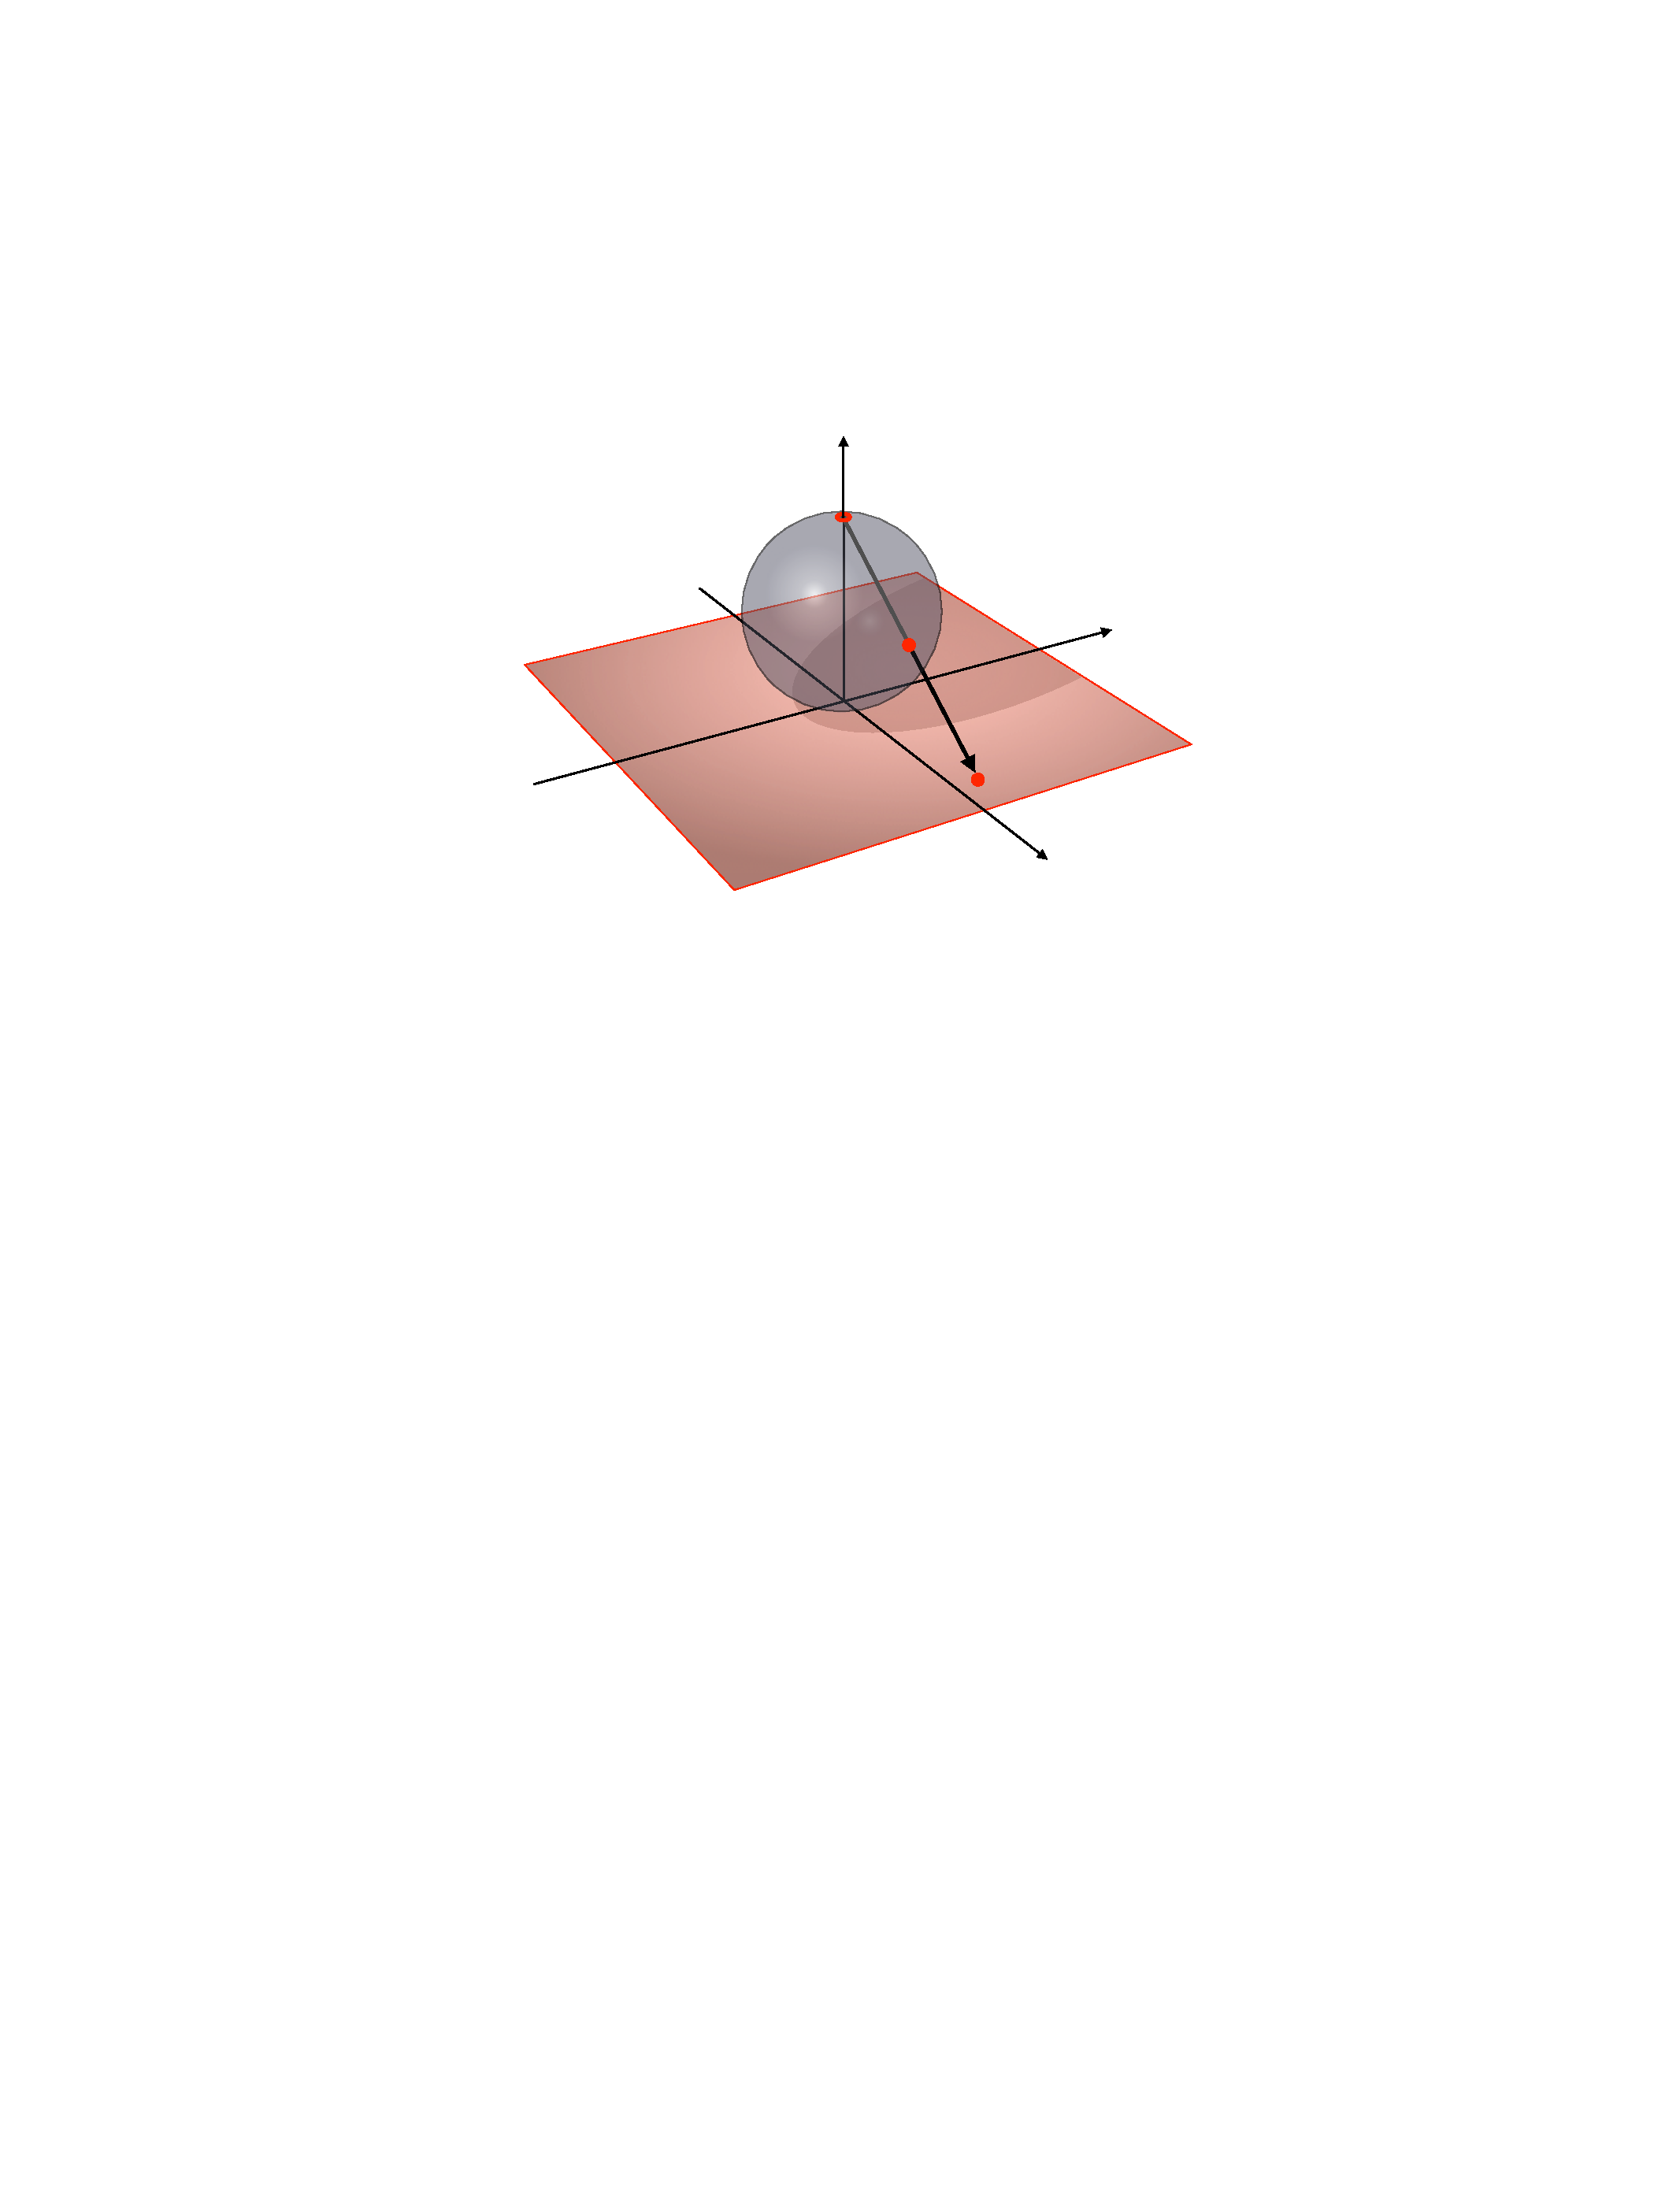
\includegraphics[width=\textwidth, trim=0mm 275mm 0mm 87mm, clip]{pictures/MTH427p001.pdf}};

%%% COORDINATE GRID
%\draw[step=0.5, help lines] (0,0) to[grid with coordinates] (15,9);
%%% 

\node at (8.9, 4.2){\small $(0, 0, 2)$};
\node at (9.1, 2.9){\small $x$};
\node at (10.0, 1.7){\small $p(x)$};
\end{tikzpicture}
%---EBLANK
\end{example}





%%%%%%%%%%%%%%%%%%%%%%%%%%%%%%%
%  EXERCISES
%%%%%%%%%%%%%%%%%%%%%%%%%%%%%%%

\exercises


\begin{exercise}
\label{Q NOT DISCR EXERCISE}
Consider  the set of rational numbers $\Q$  as a subspace of $\R$. Show that $\Q$
is not homeomorphic to a space with the discrete topology. 
\end{exercise}





\begin{exercise}
Prove Proposition \ref{SEQ FOR CONT FUNCT PROP}.
\end{exercise}




\begin{exercise}
Prove Proposition \ref{COMP CONT PROP}.
\end{exercise}




\begin{exercise}
Prove Lemma \ref{CLOSED PASTING LEMMA}.
\end{exercise}




\begin{exercise}
Prove Proposition \ref{HOMEO OPEN PROP}.
\end{exercise}




\begin{exercise}
Let $X$ be a topological space and let $f, g\colon X \to \R$ be continuous 
functions.

a) Show that the set 
$$A = \{x\in X \ | \ f(x) \geq g(x) \}$$
is closed in $X$. 

b) Let $h_{\text{max}}, h_{\text{min}}\colon X \to \R$ be a functions given by 
$h_{\text{max}}(x) = \max\{f(x), g(x)\}$ and $h_{\text{min}}(x) = \min\{f(x), g(x)\}$. 
Show that $h_{\text{max}}$  and $h_{\text{min}}$ are continuous functions. 
\end{exercise}




\begin{exercise}
Let $f, g \colon \R\to \R$ be continuous functions such that $f(x) >  g(x)$ for all $x\in \R$.
Define subspaces $X$, $Y$ of  $\R^{2}$ as follows. 
$$
X := \{ (x, y) \in \R^{2} \ | \  g(x) \leq y \leq f(x) \} \ \ \ \ \ \ \ \ 
Y:= \{(x, y) \in \R^{2} \ | \  0 \leq y \leq 1  \}
$$ 
Show that $X\cong Y$. 
\end{exercise}




\begin{exercise} 
Let  $x_{0} = (0, 0)\in \R^{2}$ and let $\xov{B}(x_{0}, 1)\subseteq \R^{2}$ be a closed
ball defined by the  Euclidean metric $d$: 
$$\xov{B}(x_{0}, 1) = \{ x\in \R^{2} \ | \ d(x, x_{0}) \leq 1 \}$$
Define subspaces $X, Y\subseteq \R^{2}$ as follows:
$$X := \R^{2}\ssmin \{x_{0}\} \ \ \ \ \ \ Y:= \R^{2}\ssmin \xov{B}(x_{0}, 1)$$
Show that $X\cong Y$.  
\end{exercise}




\begin{exercise}
\label{RETR CLOSED EXERCISE}
Let $(X, \varrho)$ be a metric space. A subspace $Y\subseteq X$ is a \emph{retract} 
of $X$ if there exists a continuous function $r\colon X\to Y$ such that $r(x) = x$ 
for all $x\in Y$. Show that if $Y\subseteq X$ is a retract of $X$ then $Y$ is a closed in $X$. 
\end{exercise}




\newpage
%%%%%%%%%%%%%%%%%%%%%%%%%%%%%%%
%%%%%%%%%%%%%%%%%%%%%%%%%%%%%%%
%%%
%%%  CONNECTEDNESS 
%%%
%%%%%%%%%%%%%%%%%%%%%%%%%%%%%%%
%%%%%%%%%%%%%%%%%%%%%%%%%%%%%%%

%---BBLANK
\chapter{Connectedness}
%---EBLANK
\chaptermark{Connectedness}

\label{CONNECTEDNESS CHAPTER}

\thispagestyle{firststyle}

%\emph{
%\begin{tabular}{@{}l@{}}
%A young man and a woman elected \\
%To get married and be so perfected. \\
%Each had an open heart  \\
%But non-empty from start  \\
%Thus their union soon proved disconnected.
%\end{tabular}
%}



\begin{nn} 
\label{CLOSED OPEN INTERV NONHOMEO NN}
Let $[a, b]\subseteq \R$ be a closed interval and let $(a, b)\subseteq \R$ be an 
open interval. We would like  to show that $[a, b]$ and $(a, b)$ are non-homeomorphic 
topological spaces. The idea of a proof of this fact is as follows. Assume that there exists a homeomorphism 
$$f\colon [a, b] \to (a, b)$$
Recall that by Proposition \ref{HOMEO PROPERTIES PROP}  for any  $Y\subseteq [a, b]$
the function $f|_{Y}\colon Y \to f(Y)$
also would  be a homeomorphism.  If we take  $Y = [a, b] \ssmin \{a \} = (a, b]$ then 
$$f(Y) = f([a, b]) \ssmin  \{f(a)\} = (a, b) \ssmin \{f(a)\}$$ 
Intuitively  the spaces $Y$ and $f(Y)$ are different in an essential way since  $Y$ comes in one 
piece while  $f(Y)$  is split into two pieces  by removal of  the point $f(a)$:
 
 \begin{equation*}
\begin{tikzpicture}[scale=1]
\begin{scope}
\fill[mypink] (0.13,0) rectangle (2.87,-0.25) ;
\draw[line width = 1.5] (0, 0) -- (3,0);
\draw[fill = white, line width = 1.5] (0, 0) circle [radius = 0.1];
\filldraw[line width = 1.5] (3, 0) circle [radius = 0.1];
\node[anchor = base] at (0.0, 0.27) {\small $a$}; 
\node[anchor = base] at (3.0, 0.27) {\small $b$}; 
\node[anchor = base] at (1.5, -1) {\small $Y = [a, b] \ssmin \{a\}$};
\end{scope}
\begin{scope}[xshift = 60mm]
\fill[mypink] (0.13,0) rectangle (1.87, -0.25) ;
\fill[mypink] (2.13,0) rectangle (2.87, -0.25) ;
\draw[line width = 1.5] (0, 0) -- (3,0);
\draw[fill = white, line width = 1.5] (0, 0) circle [radius = 0.1];
\draw[fill = white, line width = 1.5] (2, 0) circle [radius = 0.1];
\draw[fill = white, line width = 1.5] (3, 0) circle [radius = 0.1];
\node[anchor = base] at (0, 0.27) {\small $a$}; 
\node[anchor = base] at (3.0, 0.27) {\small $b$}; 
\node[anchor = base] at (2.0, 0.27) {\small $f(a)$}; 
\node[anchor = base] at (1.5, -1) {\small $f(Y) = (a, b) \ssmin \{f(a)\}$};
\end{scope}
\end{tikzpicture}
\end{equation*}

For this reason we can expect that the spaces  are $Y$ and $f(Y)$ are not homeomorphic, 
and that, as a consequence,  $[a, b]$ and $(a, b)$ are not  homeomorphic as well.  

In order to make this intuitive argument into a rigorous proof we need to define precisely what it means 
that a topological space is ``in one piece'' and then  show that this feature is  
preserved by homeomorphisms. The property of being ``in one piece'' 
is captured by the definition of a connected space:
\end{nn}

%---BBLANK # \vskip 70mm
\begin{definition}
\index{space! connected@{connected $\sim$}}
A topological space $X$ is \emph{connected} if for any  two open sets $U, V\subseteq X$
such that $U\cup V = X$ and $U, V \neq \varnothing$  we have $U\cap V \neq  \varnothing $ . 
\end{definition}
%---EBLANK

%---BBLANK # \vskip 30mm
\begin{definition}
\index{separation}
If $X$ is a topological space and $U, V\subseteq X$ are non-empty open sets such that $U\cap V = \varnothing$
and $U\cup V = X$ then we  say that $\{U, V\}$ is a \emph{separation} of $X$.  
\end{definition}
%---EBLANK

Thus, a space $X$ is connected if there does not exists a separation of $X$.   

\begin{example}
\label{INTERV WITHOUT POINT NOT CONN EX}
For $a< b$ take  $(a, b)\subseteq \R$ and let $c\in (a, b)$. 
The space $X = (a, b)\ssmin \{c\}$ is not connected. 
Indeed, the sets $U= (a, c)$ and $V= (c, b)$ form a separation of $X$. 
\end{example}

%---BBLANK # \newpage
\begin{proposition}
\label{INTERV IS CONNECT PROP}
Let $a<b$. The intervals $(a, b)$, $[a, b]$, $(a, b]$, and $[a, b)$ are connected topological 
spaces. 
\end{proposition}
%---EBLANK

\begin{proof}
Assume first that $[a, b]$ is a closed interval and that that $U, V\subseteq [a, b]$ are open sets 
such $a\in U$, $b\in V$, and $U\cup V = [a, b]$. We will show that $U\cap V \neq \varnothing$. 
Let $x_{0} = \inf V$. There are two possibilities:  either $x_{0}\not\in U$ or $x_{0}\in U$. 
In the first case  $x_{0}\in V$ and $x_{0} > a$. Since $V$ is an open set there exists $\varepsilon > 0$ 
such that $(x_{0}-\varepsilon, x_{0}+ \varepsilon)\subseteq V$. This implies that there is  $x\in V$ such that 
$x < x_{0}$ which is impossible by the definition of $x_{0}$. 

Thus the only possible option is  $x_{0}\in U$.  Since  $U$ is an open set there exists $\varepsilon' > 0$
such that  $[x_{0}, x_{0}+ \varepsilon')\subseteq U$. On the other hand, by the definition 
of $x_{0}$ we have $[x_{0}, x_{0}+ \varepsilon') \cap V \neq \varnothing$. Therefore $U\cap V \neq \varnothing$.

Assume now that $I$ is an interval (either closed, open, or half-open) and that $U, V\subseteq I$ are non-empty
open sets such that $U\cup V = I$. We will show that $U\cap V \neq \varnothing$. Let 
$c, d\in I$ be points such that $c\in U$ and $d\in V$. We can assume that $c < d$. Take
$U' = U\cap [c, d]$ and $V' = V \cap [c, d]$. The sets $U', V'$ are open in $[c, d]$, $c\in U'$, $d\in V'$, and
$U' \cup V' = [c, d]$. By the observation above we have $U'\cap V' \neq \varnothing$, and so 
$U\cap V \neq \varnothing$.  




\end{proof}

One can show that intervals are in fact the only subspaces of $\R$ that are connected:

%---BBLANK # \vfill
\begin{proposition}
\label{CONN SUBSPACES OF R PROP}
If $X$ is a connected subspace of $\R$ then $X$ is an interval (either open, closed, or half-closed, finite or
infinite). 
\end{proposition}

\begin{proof}
Exercise. 
\end{proof}
%---EBLANK


\begin{nn}
Going back to the argument outlined in \ref{CLOSED OPEN INTERV NONHOMEO NN}, by Proposition \ref{INTERV IS CONNECT PROP} we get that the space $Y = (a, b]$ is connected, and 
the space $f(Y) = (a, b) \ssmin f(a)$ is not connected by Example 
\ref{INTERV WITHOUT POINT NOT CONN EX}.  We still need to show however  
that a connected space cannot be homeomorphic to  one that is not connected. In fact a stronger statement 
is true:
\end{nn}


%---BBLANK # \newpage
\begin{proposition}
\label{CONN ONTO  MAP PROP}
Let $f\colon X\to Y$ be a continuous function. If $f$ is onto and  the space $X$ is connected 
then $Y$ is also connected. 
\end{proposition}
%---EBLANK

\begin{proof}
Assume that $Y$ is not connected and let $U, V\subseteq Y$  be a separation of $X$. 
Then the sets $f^{-1}(U), f^{-1}(V)$ form a separation of $X$ which 
contradicts the assumption that $X$ is connected. 
\end{proof}


%---BBLANK # \vskip 60mm
\begin{corollary}
\label{CONN IMAGE COR}
If $f\colon X\to Y$ is a continuous function and $X$ is a connected space then $f(X)$ is connected. 
\end{corollary}
%---EBLANK

\begin{proof}
By restricting the range of  $f$ we obtain a function 
$f\colon X \to f(X)$ which is continuous and onto, and so it we can apply
Proposition \ref{CONN ONTO  MAP PROP}. 
\end{proof}

A very useful consequence of Corollary \ref{CONN IMAGE COR} is the following fact:

%---BBLANK # \vskip 10mm
\begin{ITERMVALUE THM}
\label{ITNVAL THM}
\index{Intermediate Value Theorem}
Let $X$ be a connected topological space and let $f\colon X\to \R$ be a continuous 
function. If $a<b$ are points in $\R$ such that $a= f(x)$ and $b= f(y)$ for some 
$x, y\in X$ then for each $c\in [a, b]$ there exists $z\in X$ such that  $c= f(z)$.   
\end{ITERMVALUE THM}
%---EBLANK

\begin{proof}
By Corollary \ref{CONN IMAGE COR} the set $f(X)$ is connected, and so by  
Proposition \ref{CONN SUBSPACES OF R PROP} $f(X)$ is an interval. It follows that for any
$a, b \in f(X)$ we have $[a, b]\subseteq f(X)$. 
\end{proof}


Since every homeomorphism $f\colon X \to Y$ is onto directly from Corollary 
\ref{CONN IMAGE COR} we get:  

%---BBLANK # \vskip 50mm
\begin{corollary}
\label{CONN HOMEO INV COR}
If $X\cong Y$ and $X$ is a connected space then $Y$ is also connected. 
\end{corollary}
%---EBLANK

\begin{corollary}
The space $\R$ is connected. 
\end{corollary}

\begin{proof}
This follows from Corollary \ref{CONN HOMEO INV COR} and 
Proposition \ref{INTERV IS CONNECT PROP}  since $\R\cong (a, b)$ for any $a< b$.  
\end{proof}


%---BBLANK # \vfill
\begin{note}
\index{topological invariant}
A \emph{topological invariant} is a property of topological spaces such that if a space 
$X$ has this property and $X\cong Y$ then $Y$ also has this property. By 
Corollary \ref{CONN HOMEO INV COR} connectedness  is a topological invariant. 
\end{note}
%---EBLANK


%---BBLANK # \newpage
\begin{proposition}
\label{CONNECT EQUIV COND PROP}
Let $X$ be a topological space. The following conditions are equivalent :
\benu
\item $X$ is connected
\item For any closed sets $A, B \subseteq X$ such that $A, B \neq X$ and $A\cap B = \varnothing$
we have $A\cup B \neq X$. 
\item If $A\subseteq X$ is a set that is both open and closed then either $A= X$ or $A= \varnothing$. 
\item If $D= \{0, 1\}$ is a space with the discrete topology then any continuous function $f\colon X\to D$ is a constant function. 
\eenu
\end{proposition}

\begin{proof}
Exercise. 
\end{proof}
%---EBLANK

%---BBLANK # \vskip 10mm
\begin{proposition}
\label{UNION OF CONNECT PROP}
Let $X$ be a topological space and for $i\in I$ let $Y_{i}$ be a subspace of  $X$. Assume that 
$\bigcup_{i\in I} Y_{i} = X$ and $\bigcap_{i\in I} Y_{i} \neq \varnothing$. If $Y_{i}$ is connected
for each $i\in I$ then $X$ is also connected. 

\begin{equation*}
\begin{tikzpicture}
[scale=1.1,
contour/.style={very thick}
]
\foreach \x in {1,...,5} {
\fill[mygray3, rotate = -90+(72*(\x-1)), opacity = 0.5] 
(-1.5,-0.5) -- (0, -0.5) 
arc [radius = 0.5, start angle = -90, end angle = 90]  -- (-1.5, 0.5) 
arc [radius = 0.5, start angle = 90, end angle = 270];
}
\foreach \x in {1,...,5} {
\begin{scope}[rotate = -90+(72*(\x-1))] 
\draw
(-1.5,-0.5) -- (0, -0.5) 
arc [radius = 0.5, start angle = -90, end angle = 90]  -- (-1.5, 0.5) 
arc [radius = 0.5, start angle = 90, end angle = 270];
\node at (-1.5, 0)  {$Y_{\x}$};
\end{scope}
}
\end{tikzpicture}
\end{equation*}


\end{proposition}
%---EBLANK



\begin{proof}
Let $D= \{0, 1\}$ be a space with the discrete topology and let $f\colon X\to D$ be a continuous function. 
By Proposition \ref{CONNECT EQUIV COND PROP} it is enough to show that $f$ is a constant function. 
Let $x_{0}\in \bigcap_{i\in I} Y_{i}$. We can assume that $f(x_{0}) = 0$. For any $i\in I$ the function 
 $f|_{Y_{i}}\colon Y_{i}\to D$ is constant since $Y_{i}$ is connected.  Since  $x_{0}\in Y_{i}$ and $f(x_{0}) = 0$
we get that $f(x) =0$ for all $x\in Y_{i}$. Since this applies to all subspaces $Y_{i}$ we obtain 
 that $f(x) = 0$ for all $x\in \bigcup_{i\in I} Y_{i} = X$. 
\end{proof}


%---BBLANK # \vskip 40mm
\begin{corollary}
The space $\R^{n}$ is connected for all $n\geq 1$. 
\end{corollary}
%---EBLANK

\begin{proof}
For $0\neq x\in \R^{n}$ let $L_{x}\subseteq \R^{n}$ be the line passing through $x$ and the origin:
$$L_{x} = \{ tx\in \R^{n} \ | \ t\in \R \}$$
For every $x\in \R^{n}$ consider the  continuous function $f_{x}\colon \R \to \R^{n}$
given by $f_{x}(t) = tx$. Since $\R$ is connected and $f_{x}(\R) = L_{x}$ if follows that $L_{x}$ is connected. 
We have $\R^{n} = \bigcup_{x\in \R^{n}} L_{x}$ and $\bigcap_{x\in \R^{n}} L_{x} = \{0\}$. Therefore 
by Proposition \ref{UNION OF CONNECT PROP} the space $\R^{n}$ is connected. 
\end{proof}

%---BBLANK # \newpage
\begin{definition}
Let $X$ be a topological space. A \emph{connected component} of $X$ 
is a subspace $Y\subseteq X$ such that 
\benu
\item $Y$ is connected
\item if $Y\subseteq Z \subseteq X$ and  $Z$ is  connected then $Y= Z$. 
\eenu
\end{definition}
%---EBLANK


%---BBLANK # \vskip 30mm
\begin{proposition}
\label{CONN COMP PROP}
Let  $X$ be a topological space.
\benu
\item For every point $x_{0}\in X$ there exist a  connected component $Y\subseteq X$ such that $x_{0}\in Y$.
\item If $Y, Y'$ are connected components of $X$ then either $Y\cap Y' = \varnothing$ or $Y= Y'$.
\eenu
\end{proposition}
%---EBLANK

\begin{proof}
1)  Given a point $x_{0}\in X$ let $\{C_{i}\}_{i\in I}$ be the collection of all subspaces of $X$ such that 
$x_{0}\in C_{i}$ and $C_{i}$ is connected. Define 
$Y:= \bigcup_{i\in I} C_{i}$.
We have  $x_{0}\in Y$. Also, since $x_{0}\in \bigcap_{i\in I} C_{i}$ by  
Proposition \ref{UNION OF CONNECT PROP} we obtain that $Y$ is connected. If $Y\subseteq Z \subseteq X$
and $Z$ is connected then $Z= C_{i_{0}}$ for some $i_{0}\in I$, and so $Z =  Y$. Therefore $Y$ is a 
connected component of $X$. 

2) Let $Y$, $Y'$ be two connected components of $X$. Assume  that $Y\cap Y'\neq \varnothing$.  
By  Proposition \ref{UNION OF CONNECT PROP}  we get then that  $Y\cup Y'$ is connected. Since 
$Y\subseteq Y\cup Y'$ we must have $Y= Y\cup Y'$. By the same argument we obtain that $Y'= Y\cup Y'$. 
Therefore $Y= Y'$

\end{proof}

%---BBLANK # \vfill
\begin{corollary}
Let $X$ be a topological space. If $Z\subseteq X$ is a connected subspace then there exists a
connected component $Y\subseteq X$ such that $Z\subseteq Y$. 
\end{corollary}

\begin{proof}
Exercise.
\end{proof}

\begin{corollary}
Let $f\colon X\to Y$ be a continuous function. If $X$ is a connected space 
then there exists a connected component $Z\subseteq Y$ such that $f(X)\subseteq Z$. 
\end{corollary}

\begin{proof}
Exercise.
\end{proof}
%---EBLANK


%%%%%%%%%%%%%%%%%%%%%%%%%%%%%%%
%  EXERCISES
%%%%%%%%%%%%%%%%%%%%%%%%%%%%%%%

\exercises

\begin{exercise}
\label{DENSE CONNECTED SUBSP EXERCISE}
Let $X$ be a topological space and let $Y\subseteq X$ be a subspace. Show that 
if $Y$ is a connected space and $Y$ is dense in $X$ then $X$ is connected. 
\end{exercise}



\begin{exercise}
Prove Proposition \ref{CONN SUBSPACES OF R PROP}. 
\end{exercise}




\begin{exercise}
\label{SPHERES CONNECTED EXERCISE}
Show that the sphere $S^{n}$ is connected for all $n \geq 1$. 
\end{exercise}




\begin{exercise}
Let $a<b$. Show that the closed interval $[a, b]\subseteq \R$ is not homeomorphic
to the half-closed interval $(a, b]$. 
\end{exercise}




\begin{exercise}
Let $a<b$. Show that the circle $S^{1}$ is not homeomorphic to any of the intervals:
$(a, b)$, $[a, b]$, $[a, b)$. 
\end{exercise}








\begin{exercise}
A function $f\colon \R\to \R$ is \emph{strictly increasing} is for all $x, y\in \R$ such that $x> y$ we have 
$f(x) > f(y)$, and is it \emph{strictly decreasing} is for all $x, y\in \R$ such that $x> y$ we have 
$f(x) < f(y)$. Show that if $f\colon \R\to\R$ is a continuous 1-1 function then $f$ is either strictly increasing 
or strictly decreasing. 
\end{exercise}






\begin{exercise}
Let $f\colon \R \to \R$ be a continuous function such that $f(x)\cdot f(f(x)) = 1$ for all $x\in \R$ and that 
$f(10) = 9$. Find the value of $f(5)$. Justify your answer.  
\end{exercise}




\begin{exercise}
Let $f\colon S^{n} \to \R$ be a continuous function. Show that there exists a point $x\in S^{n}$
such that $f(x) = f(-x)$. Here if $x = (x_{1}, \dots, x_{n})\in S^{n}$ then $-x = (-x_{1}, \dots, -x_{n})$. 
\end{exercise}





\begin{exercise}
Let $a< b$. Show that there does not exist a continuous bijection $f\colon (a, b) \to [a, b]$. 
Remember  that a continuous bijection need not be a homeomorphism since the inverse function 
may be not continuous (see \ref{CONT BIJ NOTE}).
\end{exercise}




\begin{exercise}
Prove Proposition \ref{CONNECT EQUIV COND PROP}. 
\end{exercise}




\begin{exercise}
Let $X$ be a topological space. Show that the following conditions are equivalent:
\benu
\item $X$ is connected 
\item if $A\subseteq X$ is any set such that $A\neq X$ and $A\neq \varnothing$ then $\Bd(A)\neq \varnothing$. 
\eenu
\end{exercise}





\begin{exercise}
Let $X$ be a topological space. Show that every connected component of $X$ is closed in $X$.  
\end{exercise}



\begin{exercise}
Let $(X, \varrho)$ be a metric space. Assume for some $x_{0}\in X$ and $r>0$ the open ball $B(x_{0}, r)$
consists of countably many points. Show that $X$ is not connected. 
\end{exercise}





\begin{exercise}
Let $X$ be the subspace of $\R^{2}$ consisting of the positive $x$-axis and of the graph of the function 
$f(x) = \tfrac{1}{x}$ for $x> 0$:
$$X := \{(x, 0)\in \R^{2} \ | \ x > 0\} \cup \{(x, \tfrac{1}{x}) \in \R^{2} \ | \ x>0  \}$$
\begin{equation*}
\begin{tikzpicture}[scale =1] 
\draw[->, >=latex, thick] (-0.3,0.2) -- (3.8,0.2);
\draw[->, >=latex, thick] (0.2,-0.3) -- (0.2,3.3) ;
\draw[line width = 2 , domain= 0.33:3.5,smooth,variable=\x, red, samples = 50] plot ({\x},{1/\x});
\draw[red, line width = 2] (0.2,0.2) -- (3.5, 0.2);
\end{tikzpicture}
\end{equation*}

Show that $X$ is not connected. 
\end{exercise}





\begin{exercise}
\label{SINE CURVE CONN EXERCISE}
\index{topologist's sine curve}
The \emph{topologist's sine curve} is the subspace 
 $Y$  of $\R^{2}$ that consists of a segment of the $y$-axis and of the graph
of the function $f(x) = \sin(\tfrac{1}{x})$:
$$Y := \{(0, y)\in \R^{2} \ | \ -1 \leq y\leq 1\} \cup \{(x, \sin(\tfrac{1}{x})) \in \R^{2} \ | \ x>0  \}$$
\begin{equation*}
\begin{tikzpicture}[scale =1] 
\draw[->, >=latex, thick] (1.5,0) -- (7,0);
\draw[->, >=latex, thick] (2.1,-1.4) -- (2.1,1.4) ;
\draw[line width = 2, red] (2.1, -1.03) -- (2.1, 1.03);
\begin{scope}
\clip (1.5, -1.2) rectangle (7, 1.2);
\draw[xscale=15, line width = 2 , domain= 0.151:0.5,smooth,variable=\x, red, samples = 400] plot ({\x},{sin(pow(\x, -2) r)});
\end{scope}
\end{tikzpicture}
\end{equation*}
Show that $Y$ is  connected. 
\end{exercise}




\begin{exercise}
Let $f, g\colon \R\to \R$ be continuous functions such that $g(x) \leq f(x)$ for all $x\in \R$. 
Let $Z$ be the subspace of $\R^{2}$ given by 
$$Z = \{(x, y) \ | \ g(x) \leq y \leq f(x) \}$$
\begin{equation*}
\begin{tikzpicture}[scale =1] 
\begin{scope}
\clip
(-0.5, -0.5) 
.. controls (0, -0.2) and (1, -1.5) .. (1.5, -1.5)
.. controls (2.2, -1.5) and (2.2, -0.5) .. (2.5, -0.5)
.. controls (2.6, -0.5) and (2.7, -0.7) .. (3.0, -0.7)
.. controls (3.5, -0.7) and (3.8, 0.4) .. (4.2, 0.4)
.. controls (4.5, 0.4) and (4.8, -0.4) .. (5, -0.4)
-- (5, 1.5) -- (-0.5, 1.5) -- cycle;
\fill[mypink, opacity = 0.8] 
(-0.5, 0.5) 
.. controls (0, 0.6) and (0.25, 1) .. (0.5, 1)
.. controls (1, 1) and (1.2, -0.5) .. (1.5, -0.5)
.. controls (1.8, -0.5) and (2,  0.5) .. (2.3,  0.5)
.. controls (2.6,  0.5) and (2.5,  -0.7) .. (3,  -0.7)
.. controls (3.5,  -0.7) and (3.5,  1) .. (4.2,  1)
.. controls (4.5,  1) and (4.9,  0.8) .. (5,  0.8)
-- (5, -1.5) -- (-0.5, -1.5) -- cycle;
\end{scope}

\begin{scope}
\clip (-0.5, -1.7) rectangle (5, 1.7);
\draw[line width = 1.5, red] 
(-0.6, 0.5) 
.. controls (0, 0.6) and (0.25, 1) .. (0.5, 1)
.. controls (1, 1) and (1.2, -0.5) .. (1.5, -0.5)
.. controls (1.8, -0.5) and (2,  0.5) .. (2.3,  0.5)
.. controls (2.6,  0.5) and (2.5,  -0.7) .. (3,  -0.7)
.. controls (3.5,  -0.7) and (3.5,  1) .. (4.2,  1)
.. controls (4.5,  1) and (4.9,  0.8) .. (5,  0.8)
(-0.6, -0.5) 
.. controls (0, -0.2) and (1, -1.5) .. (1.5, -1.5)
.. controls (2.2, -1.5) and (2.2, -0.5) .. (2.5, -0.5)
.. controls (2.6, -0.5) and (2.7, -0.7) .. (3.0, -0.7)
.. controls (3.5, -0.7) and (3.8, 0.4) .. (4.2, 0.4)
.. controls (4.5, 0.4) and (4.8, -0.4) .. (5, -0.4)
;
\end{scope}
\draw[->, >=latex, thick] (-0.5,0) -- (5.3,0);
\draw[->, >=latex, thick] (0, -1.7) -- (0, 1.7) ;
\node[anchor= base east] at (5.2, 1.3) {\small \color{red} $y = f(x)$};
\node[anchor= base east] at (5.2, -0.9) {\small \color{red} $y = g(x)$};
\node[anchor= base west] at (0.2,  0.2) {\small \color{red} $Z$};
\end{tikzpicture}
\end{equation*}

Show that $Z$ is  connected. 
\end{exercise}






\begin{exercise}
Consider the unit circle $S^{1} = \{ (x, y)\in \R^{2} \  | \  x^{2} + y^{2} = 1\}$. 
Let $p\colon \R\to S^{1}$ denote the function 
given by  $p(t) = (\sin 2\pi t, \cos 2\pi  t)$. 
Geometrically speaking this function wraps $\R$ infinitely many times  around the circle:

\begin{tikzpicture}
\node[anchor=south west,inner sep=0] at (0,0) 
{{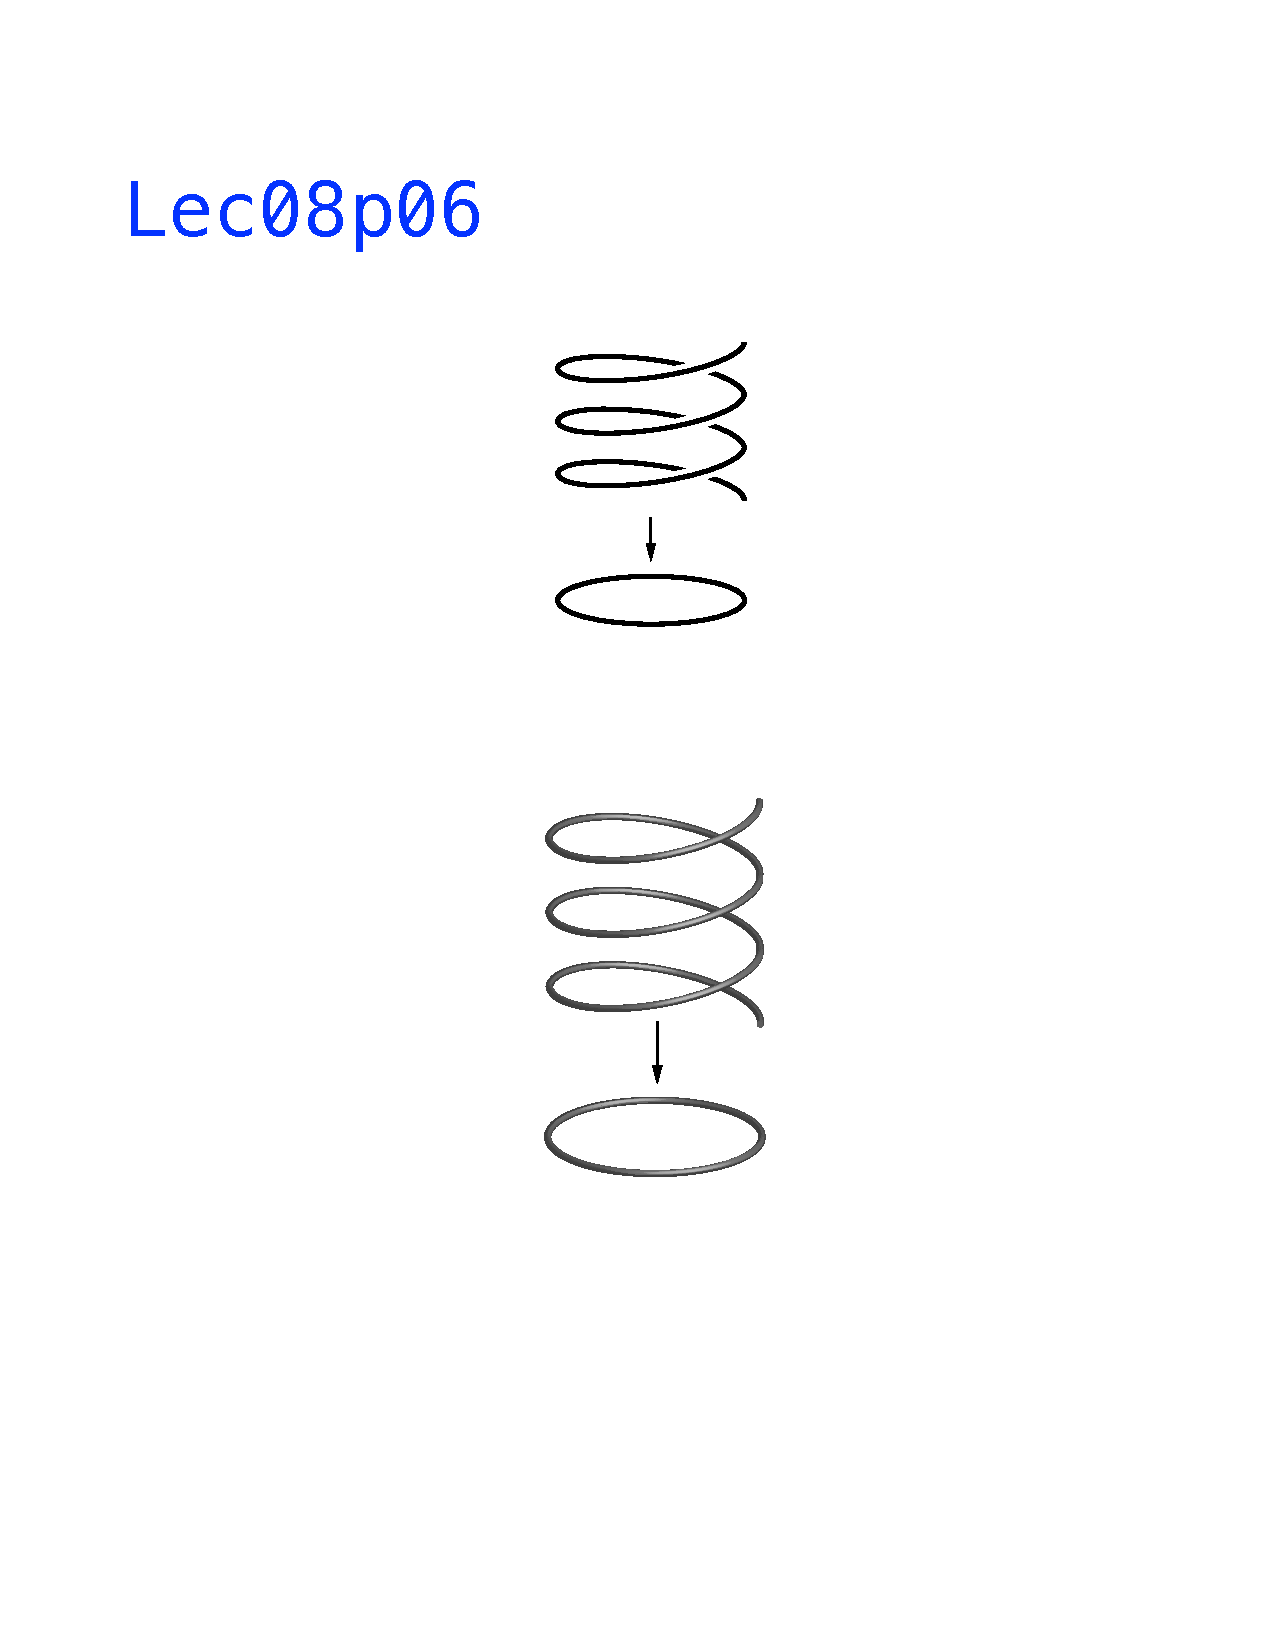
\includegraphics[width=\textwidth, trim=0mm 173mm 0mm 57mm, clip]{pictures/MTH427p002.pdf}}};

%%% COORDINATE GRID
%\draw[step=0.5, help lines] (0,0) to[grid with coordinates] (15,9);
%%% 

\node[anchor = base west]  at (9.65, 3.5){\small $\R$};
\node[anchor = base west] at (9.65, 0.4){\small $S^{1}$};
\node at (8.7,1.25){\small $p$};
\end{tikzpicture}

Show that there does not exist 
a continuous function $g\colon S^{1} \to \R$ such that $pg = \id_{S^{1}}$. 
\end{exercise}






\begin{exercise}
\label{Q TOTALY DISCONNECT EXERCISE}
\index{space! totally disconnected@{totally disconnected $\sim$}}
A space $X$ is \emph{totally disconnected} if every connected component of $X$ consists of a single 
point. Obviously every discrete topological space is totally disconnected. Consider the set ot rational numbers 
$\Q$ as a subspace of $\R$. Show that $\Q$ is totally disconnected. Note that  by Exercise 
\ref{Q NOT DISCR EXERCISE} $\Q$ is not a discrete space.  
\end{exercise}






\begin{exercise}
Show that metrizability is a topological invariant. That is, it $X$ and $Y$ are homeomorphic spaces, and
$X$ metrizable then so is $Y$.   
\end{exercise} 





\newpage
%%%%%%%%%%%%%%%%%%%%%%%%%%%%%%%
%%%%%%%%%%%%%%%%%%%%%%%%%%%%%%%
%%%
%%%  PATH CONNECTEDNESS
%%%
%%%%%%%%%%%%%%%%%%%%%%%%%%%%%%%
%%%%%%%%%%%%%%%%%%%%%%%%%%%%%%%

%---BBLANK
\chapter[Path Connectedness]{Path \\ Connectedness}
%---EBLANK 


The notion of connectedness of a space was invented to define rigorously what 
it means that a space is ``in one piece''. In this chapter we introduce path connectedness 
which is designed to capture a similar property but in a different way. It turns out that these 
two notions are not the same: while every path connected space is connected, the opposite 
is not true. In effect path connectedness gives us a new topological invariant of spaces. 
Additional related invariants are obtained by considering local connectedness and local path 
connectedness of spaces. 

\thispagestyle{firststyle}


%---BBLANK 
\begin{definition}
\index{path}
Let $X$ be a topological space. A \emph{path} in $X$ is a continuous function 
$\omega\colon [0, 1] \to X$. If $\omega(0) = x_{0}$ and $\omega(1) = x_{1}$
then we say that $\omega$ joins $x_{0}$ with $x_{1}$. 

\begin{equation*}
\begin{tikzpicture}[scale =1] 
\begin{scope}
\draw[red, line width = 1.5]
(0, 1.5) -- (2, 1.5);
\fill[red] (0, 1.5) circle (0.07) node[below] {\color{black} \small 0}; 
\fill[red] (2, 1.5) circle (0.07) node[below] {\color{black} \small 1}; 
\end{scope}
\begin{scope}[xshift = 30mm]
\draw[->, >=latex, thick] (0, 1.5) to[out = 40, in = 140] node[above] {\small $\omega$} (1.8, 1.5);
\end{scope}
\begin{scope}[xshift = 55mm]
\draw[fill = mygray2]
(0.4 , 1)
.. controls +(0, -1) and +(-0.2, 0) .. 
(1.5 , 0)
.. controls +(0, 0) and +(0, -1) .. 
(2.7, 1)
.. controls +(0, 0.5) and +(1, 0).. 
(2.1, 2.8)
.. controls +(-0.9, 0) and +(-0.2, 0.5).. 
(1.25, 1.6)
.. controls +(0.1, -0.25) and +(0.2, 0).. 
(1.1, 1)
.. controls +(-0.2, 0) and +(-0.2, -0.5).. 
(0.9, 1.6)
.. controls +(0.2, 0.5) and +(0.5, 0).. 
(0.7, 2.8) 
.. controls +(-0.9, 0) and +(0, 0.5).. 
(0.4, 1) 
;
\draw[fill = white, scale = 0.42, xshift= 38mm, yshift = 56mm, rotate= -110] 
plot [smooth cycle, tension = 0.85] coordinates{(0.55, 2.0) (0.65, 0.55)  (2.25, 0.47) (2.5, 2.4)};
\draw[fill = white] (1.35, 0.45) circle (0.3);

\draw[red, line width = 1.5pt] 
(0.6, 2.2) 
.. controls +(0, -0.1) and +(0, 0.3) .. 
(0.6, 1.2)
.. controls +(0, -0.5) and +(-0.1, -0.04) ..
(1.1 , 0.85) 
.. controls +(0.5, +0.2) and +(-0.2, 0) ..
(2.0, 0.7)
.. controls +(0.3, 0) and +(0, -0.4) ..
(2.55, 1.5)
.. controls +(0, 0.4) and +(0.7, 0.2)  ..
(1.7, 2.2)
;
\draw[->, >=angle 60, red, very thick, rotate around={-19:(2.0, 0.7)}] (2.0, 0.7) -- (2.01, 0.7);
\fill (0.6, 2.2)  circle (0.07) node[above] {\small $x_{0}$};
\fill (1.7, 2.2)  circle (0.07) node[above] {\small $x_{1}$};
\end{scope}
\end{tikzpicture}
\end{equation*}
\end{definition}
%---EBLANK


%---BBLANK # \newpage
\begin{definition}
\index{path! inverse of@{inverse of $\sim$}}
1) If $\omega\colon [0, 1] \to X$ is a path in $X$ then the \emph{inverse} of $\omega$ is the 
path $\xov{\omega}$ given by $\xov{\omega}(t) = \omega(1-t)$ for $t\in [0, 1]$. 

\begin{equation*}
\begin{tikzpicture}
\draw (0, 0.2) rectangle (4, 2.2);

% Draw curved path
\draw[mygray5, line width = 1.6pt]
(0.5, 0.5) 
.. controls +(0.5, 1.3) and +(-0.5, 1.3) ..
(3.5, 0.5)  {\foreach \i in {1,...,40} {  coordinate[pos= \i/40] (p\i) } };;

\draw[->, >=angle 60, white, very thick, rotate around={12:($(p15)!1.5pt!90:(p16)$)}] 
($($(p15)!1.5pt!90:(p16)$)!0.25!($(p16)!1.5pt!90:(p17)$)$) -- +(-0.01, 0); 
\draw[->, >=angle 60, white, very thick, rotate around={12:($(p15)!1.5pt!90:(p16)$)}] 
($($(p15)!1.5pt!90:(p16)$)!0.25!($(p14)!1.5pt!90:(p15)$)$) -- +(-0.06, 0); 




% Draw parallel curve
% (note that first and last points are specified out of the loop)
\draw[red, line width = 1.6pt] ($(0.5, 0.5)!1.5pt!90:(p2)$) 
{ \foreach \i [count=\j from 2] in {1,...,39} {-- ($(p\i)!1.5pt!90:(p\j)$) } }
 -- ($(p40)!1.5pt!-90:(p39)$);
 
 

 \draw[->, >=angle 60, white,very thick, rotate around={-12:(p3)}] ($(p25)!0.25!(p26)$) -- +(0.07, 0); 
  \draw[->, >=angle 60, white,very thick, rotate around={-12:(p3)}] ($(p25)!0.25!(p24)$) -- +(0.01, 0); 
 
 \begin{scope}
 \clip (p25) circle (0.5); 
 \draw[mygray5, line width = 1.6pt]
(0.5, 0.5) 
.. controls +(0.5, 1.3) and +(-0.5, 1.3) ..
(3.5, 0.5); 
 \end{scope}
 
 
 \draw[white, line width = 0.4pt] ($(0.5, 0.5)!0.75pt!90:(p2)$) 
{ \foreach \i [count=\j from 2] in {1,...,39} {-- ($(p\i)!0.75pt!90:(p\j)$) } }
 -- ($(p40)!0.75pt!-90:(p39)$);


\draw[->, >=angle 60, mygray5, very thick, rotate around={-12:(p25)}] (p25) -- +(0.035, 0); 
\draw[->, >=angle 60, red, very thick, rotate around={12:($(p15)!1.5pt!90:(p16)$)}] ($(p15)!1.5pt!90:(p16)$) -- +(-0.035, 0); 

\fill[xshift = -0.75pt] (0.5, 0.5) circle (0.07);
\fill[xshift = 0.75pt] (3.5, 0.5) circle (0.07);
\node at (0.3, 1.9) {\small $X$};
\node at (2, 1.2) {\small \color{mygray5} $\omega$};
\node at (2, 1.8) {\small \color{red} $\xov\omega$};
\end{tikzpicture}
\end{equation*}



\index{path! concatenation@{$\sim$ concatenation}}
\index{concatenation of paths}
2) If $\omega. \tau\colon [0, 1] \to X$ are paths such that $\omega(1) = \tau(0)$ then the 
\emph{concatenation} of $\omega$ and $\tau$ if the path $\omega\ast\tau$ given by 
$$
(\omega\ast\tau)(t) = 
\begin{cases}
\omega(2t) & \text{ for $t\in [0, \nicefrac{1}{2}]$} \\
\tau(2t-1)  & \text{ for $t\in [\nicefrac{1}{2}, 1]$} \\
\end{cases}
$$

\begin{equation*}
\begin{tikzpicture}
\draw (0, 0) rectangle (4, 2);
\draw[red, line width = 1.5pt]
(0.5, 0.5) 
.. controls +(0, 0.5) and +(-0.5, 0) ..
(2, 1.5) coordinate[midway] (a1);
\draw[red, line width = 1.5pt]
(2, 1.5)
.. controls +(0, -0.7) and +(-0.5, 0) ..
(3.5, 0.5) coordinate[midway] (a2);
\draw[->, >=angle 60, red, very thick, rotate around={32:(a1)}] (a1) -- +(0.01, 0) 
node[anchor = north west, xshift = -4] {\small \color{red} $\omega$};
\draw[->, >=angle 60, red, very thick, rotate around={-30:(a2)}] (a2) -- +(0.01, 0)
node[anchor = south west, xshift = -4] {\small \color{red} $\tau$};
\fill (0.5, 0.5) circle (0.07);
\fill (2, 1.5) circle (0.07);
\fill (3.5, 0.5) circle (0.07);
\node at (0.3, 1.7) {\small $X$};
\end{tikzpicture}
\end{equation*}
\end{definition}
%---EBLANK


%---BBLANK # \vskip 30mm
\begin{definition}
\label{PATH CONN DEF}
\index{space!path connected@{path connected $\sim$}}
A space $X$ is \emph{path connected} if for every $x_{0}, x_{1}\in X$ there is a path
joining $x_{0}$ with $x_{1}$.
\end{definition}
%---EBLANK


\begin{example}
For any $n\geq 1$ the space $\R^{n}$ is path connected. Indeed, if $x_{0}, x_{1}\in \R^{n}$
then define $\omega\colon [0, 1]\to \R^{n}$ by 
$$\omega(t) = (1-t)x_{0} +  tx_{1}$$
We have $\omega(0) = x_{0}$ and $\omega(1) = x_{1}$. 
\end{example}


%---BBLANK # \vfill
\begin{proposition}
\label{PATHCONN IS CONN PROP}
Every path connected space is connected.
\end{proposition}

\begin{proof}
Exercise. 
\end{proof}
%---EBLANK

\begin{note}
\label{TOPOLOGIST SIN NOT PATH CONN NOTE}
It is not true that a connected space must be path connected. For example,  let 
$Y$ be the topologist's sine curve (\ref{SINE CURVE CONN EXERCISE}). 
This is a connected space. On the other hand  $Y$ is not path connected (exercise). 
\end{note}


%---BBLANK # \newpage
\begin{proposition}
\label{UNION OF PATH CONN PROP}
Let $X$ be a topological space and for $i\in I$ let $Y_{i}$ be a subspace of  $X$. Assume that 
$\bigcup_{i\in I} Y_{i} = X$ and $\bigcap_{i\in I} Y_{i} \neq \varnothing$. If $Y_{i}$ is path 
connected for each $i\in I$ then $X$ is also path connected. 
\begin{equation*}
\begin{tikzpicture}
[scale=1.1,
contour/.style={very thick}
]
\foreach \x in {1,...,5} {
\fill[mygray3, rotate = -90+(72*(\x-1)), opacity = 0.5] 
(-1.5,-0.5) -- (0, -0.5) 
arc [radius = 0.5, start angle = -90, end angle = 90]  -- (-1.5, 0.5) 
arc [radius = 0.5, start angle = 90, end angle = 270];
}
\foreach \x in {1,...,5} {
\begin{scope}[rotate = -90+(72*(\x-1))] 
\draw
(-1.5,-0.5) -- (0, -0.5) 
arc [radius = 0.5, start angle = -90, end angle = 90]  -- (-1.5, 0.5) 
arc [radius = 0.5, start angle = 90, end angle = 270];
\node at (-1.5, 0)  {$Y_{\x}$};
\end{scope}
}
\end{tikzpicture}
\end{equation*}
\end{proposition}
%---EBLANK

\begin{proof}
Let $x_{0}, x_{1}\in X$. We need to show that there exists a path $\omega\colon [0, 1]\to X$
such that $\omega(0) = x_{0}$ and $\omega(1) = x_{1}$. 

Since $X= \bigcup_{i\in I} Y_{i}$ we have $x_{0}\in Y_{i_{0}}$ and $x_{1}\in Y_{i_{1}}$ for some
$i_{0}, i_{1}\in I$. Let $y\in \bigcap_{i\in I} Y_{i}$. Since $Y_{i_{0}}$ is path connected and 
$x_{0}, y\in Y_{i_{0}}$ there is a path $\sigma \colon [0, 1]\to Y_{i_{0}}$ such that $\sigma(0) = x_{0}$
and $\sigma(1) = y$.  Also, since $Y_{i_{1}}$ is path connected and 
$x_{1}, y\in Y_{i_{1}}$ there is a path $\tau \colon [0, 1]\to Y_{i_{1}}$ such that $\tau(0) = y$
and $\tau(1) = x_{1}$. The concatenation $\sigma\ast \tau$ gives a path joining $x_{0}$ with $x_{1}$. 
\begin{equation*}
\begin{tikzpicture}
[scale=1.1,
contour/.style={very thick}
]
\foreach \x in {1,...,5} {
\fill[mygray2, rotate = -90+(72*(\x-1))] 
(-1.5,-0.5) -- (0, -0.5) 
arc [radius = 0.5, start angle = -90, end angle = 90]  -- (-1.5, 0.5) 
arc [radius = 0.5, start angle = 90, end angle = 270];
}
\foreach \x in {1,...,5} {
\begin{scope}[rotate = -90+(72*(\x-1))] 
\draw
(-1.5,-0.5) -- (0, -0.5) 
arc [radius = 0.5, start angle = -90, end angle = 90]  -- (-1.5, 0.5) 
arc [radius = 0.5, start angle = 90, end angle = 270];
\end{scope}
}
\draw[red, very thick, postaction= {decorate, decoration={markings, mark=at position 0.55 with {\arrow{angle 60}}}}] 
(-1.4, 0.4) 
.. controls (-1.1, 0.7) and  (-0.7, 0.25) .. (-0.7, 0.25)
.. controls (-0.7, 0.25) and (-0.4, -0.1) .. (0, 0);
\draw[red, very thick] 
(0, 0) 
.. controls (0, 0) and  (0.5, -0.2) .. (0.5, -0.7)
.. controls (0.5, -1.2) and (0.9, -1.2) .. (0.9, -1.2);
\fill (0, 0) circle (0.07) node[above] {\small $y$}; 
\fill (-1.4, 0.4) circle (0.07) node[above] {\small $x_{0}$};
\fill (0.9, -1.2) circle (0.07) node[below] {\small $\ x_{1}$};
\node at (-0.85, 0.05) {\small \color{red} $\sigma$};
\node at (0.68, -0.7) {\small \color{red} $\tau$};
\draw[->, >=angle 60, red, very thick, rotate around={-85:(0.5, -0.7)}] (0.5, -0.7) -- (0.501, -0.7);
\node at (-2.25, 0.5) {\small $Y_{i_{1}}$};
\node at (1.75, -1.3) {\small $Y_{i_{2}}$};
\end{tikzpicture}
\end{equation*}
\end{proof}


%---BBLANK # \vskip 30mm
\begin{definition}
Let $X$ be a topological space. A \emph{path connected component} of $X$ 
is a subspace $Y\subseteq X$ such that 
\benu
\item $Y$ is path connected
\item if $Y\subseteq Z \subseteq X$ and  $Z$ is  path connected then $Y= Z$. 
\eenu
\end{definition}
%---EBLANK

%---BBLANK # \vskip 30mm
\begin{proposition}
\label{PATH CONN COMP PROP}
Let  $X$ be a topological space.
\benu
\item For every point $x_{0}\in X$ there exist a  path connected component $Y\subseteq X$ such that $x_{0}\in Y$.
\item If $Y, Y'$ are path connected components of $X$ then either $Y\cap Y' = \varnothing$ or $Y= Y'$.
\eenu
\end{proposition}


\begin{proof}
Similar to  the proof of Proposition \ref{CONN COMP PROP}.
\end{proof}
%---EBLANK


%---BBLANK # \newpage
\begin{proposition}
\label{PATH CONN COMP VIA PATHS PROP}
Let $x_{0}\in X$ The path connected component $Y\subseteq X$ that contains $x_{0}$ is given by: 
$$Y = \{x\in X \ | \ \text{there exists a path joining $x$ with $x_{0}$} \}$$
\end{proposition}

\begin{proof}
Exercise.
\end{proof}
%---EBLANK

%---BBLANK # \vskip 50mm
\begin{example}
\index{topologist's sine curve}
Let $Y$ be the topologist's sine curve. The space $Y$ has only one connected component 
(since $Y$ is connected). On the other hand it has two path connected components:
$$Y_{1} = \{(0, y) \ | \ -1\leq y \leq 1\} \text{ \ \ \ and \ \ \ } Y_{2} = \{(x, \sin(\tfrac{1}{x}))  \ | \ x>0  \}$$
\begin{equation*}
\begin{tikzpicture}[scale =1] 
\draw[red, line width = 1.5] (2.1, -1.03) -- (2.1, 1.03);
\begin{scope}
\draw[xscale=15, line width = 1.5 , domain= 0.151:0.4,smooth,variable=\x, samples = 800] plot ({\x},{sin(pow(\x, -2) r)});
\end{scope}
\node at (1.8, 0.88){\small $\color{red} Y_{1}$};
\node at (5.9, 0.88){\small $ Y_{2}$};
\end{tikzpicture}
\end{equation*}


\end{example}
%---EBLANK


%---BBLANK # \newpage
\begin{definition}
Let $X$ be a topological space. 

1)  $X$ is \emph{locally connected} if for any $x\in X$ and any open neighborhood $U$ of $x$
there is an  open neighborhood $V$ of $x$ such that $V\subseteq U$ and $V$ is connected.

2)  $X$ is \emph{locally path connected} if for any $x\in X$ and any open neighborhood $U$ of $x$
there is an  open neighborhood $V$ of $x$ such that $V\subseteq U$ and $V$ is path connected.

\end{definition}
%---EBLANK

\begin{example}
Let $X = (0, 1) \cup (2, 3) \subseteq \R$. The space $X$ is neither connected nor path connected 
but it is both locally connected and locally path connected. 
\end{example}


\begin{example}

Let $X$ be the subspace of $\R^{2}$ consisting of the intervals joining points 
$(0, 0)$ and $(\nicefrac{1}{n}, 0)$ for $n=1, 2, \dots$ with the point $(0, 1)$:

\begin{equation*}
\begin{tikzpicture}[scale =1] 
\fill (0, 2) circle (0.07) node[left = 2pt] {\small $(0, 1)$};
\fill (0, 0) circle (0.07) node[left = 2pt] {\small $(0, 0)$};
\fill (4.5, 0) circle (0.07);
\fill (3, 0) circle (0.07);
\fill (2, 0) circle (0.07);
\fill (1.2, 0) circle (0.07);
\fill (0.75, 0) circle (0.07);
\fill (0.35, 0) circle (0.07);
\draw[line width = 1.5]
(0,2) -- (0, 0) 
(0,2) -- (4.5, 0) 
(0,2) -- (3, 0)
(0,2) -- (2, 0) 
(0,2) -- (1.2, 0)
(0,2) -- (0.75, 0)
(0,2) -- (0.35, 0);
\end{tikzpicture}
\end{equation*}
\index{harmonic broom}
The space $X$ is called the \emph{harmonic broom}. This space is connected and 
path connected. It is neither locally connected nor locally path connected since any neighborhood 
of the point $(0, 0)$ that does not contain the point $(0, 1)$ is not connected. 
\end{example}



%---BBLANK # \newpage
\begin{proposition}
\label{LOC PCONN IS LOC CONN PROP}
If $X$ is locally path connected then it is locally connected. 
\end{proposition}

\begin{proof}
Exercise. 
\end{proof}

\begin{proposition}
\label{LOC CONN COMP OPEN PROP}
If a space $X$ is locally  connected then connected components of $X$ are open in $X$. 
\end{proposition}

\begin{proof}
Exercise. 
\end{proof}

\begin{proposition}
\label{LOC PCONN COMP OPEN PROP}
If a space $X$ is locally  path connected then path connected components of $X$ are open in $X$. 
\end{proposition}

\begin{proof}
Exercise.
\end{proof}

\begin{proposition}
\label{CONN AND LOC PATH CONN IS PATH CONN PROP}
If $X$ is a connected and locally path connected space then $X$ is path connected.  
\end{proposition}
%---EBLANK

\begin{proof}
It is enough to show that  $X$ has only one path connected component. Assume, by contradiction, 
that $X$ has at least two distinct path connected components. Let $Y$ be some path connected component 
of $X$ and let $Y'$ be the union of all other path connected components. By Proposition  
\ref{LOC PCONN COMP OPEN PROP} both $Y$ and $Y'$ are open sets. Also $Y\cap Y' = \varnothing$
and $Y\cup Y' =  X$. This contradicts the assumption that $X$ is connected.   
\end{proof}


%%%%%%%%%%%%%%%%%%%%%%%%%%%%%%%
%  EXERCISES
%%%%%%%%%%%%%%%%%%%%%%%%%%%%%%%

\exercises


\begin{exercise}
Prove Proposition \ref{PATHCONN IS CONN PROP}. 
\end{exercise}




\begin{exercise}
Prove Proposition \ref{PATH CONN COMP VIA PATHS PROP}. 
\end{exercise}




\begin{exercise}
The goal of this exercise is to verify that the statement of Note \ref{TOPOLOGIST SIN NOT PATH CONN NOTE}
holds.  Show that the topologist sine curve (Exercise \ref{SINE CURVE CONN EXERCISE}) is not path connected. 
\end{exercise}




\begin{exercise}
Let $X$ be a topological space whose elements are integers, and such that $U\subseteq X$
is open if either $U = \varnothing$ or $U = X\ssmin S$ for some finite set $S$. Show that 
$X$ is locally connected but not locally path connected. 
\end{exercise}




\begin{exercise}
Prove Proposition \ref{LOC CONN COMP OPEN PROP}. 
\end{exercise}



\begin{exercise}
Prove Proposition \ref{LOC PCONN COMP OPEN PROP}.
\end{exercise}







\begin{exercise}
Let $M_{n}(\R)$ denote the set of all $n\times n$ matrices with coefficients in $\R$. Since 
each matrix consists of $n^{2}$ real numbers the set $M_{n}(\R)$ can be identified with $\R^{n^{2}}$.
Using this identification we can consider $M_{n}(\R)$ as a topological space. Let $GL_{n}(\R)$ be the 
subspace of $M_{n}(\R)$ consisting of all invertible matrices. Equivalently:
$$GL_{n}(\R) = \{ A\in M_{n}(\R) \ | \ \det A \neq 0\}$$
where $\det A$ is the determinant of $A$. Show that $GL_{n}(R)$ has exactly two path connected components:
$GL_{n}^{+}(\R)$ and $GL_{n}^{-}(\R)$ where 
$$GL_{n}^{+}(\R) = \{ A\in GL_{n}(R) \ | \ \det A > 0\}, \ \ \ \ 
GL_{n}^{-}(\R) = \{ A\in GL_{n}(R) \ | \ \det A < 0\}$$
\end{exercise}







\begin{exercise}
\label{OPEN CONN IN RN IS PATH EXERCISE}
Let $X$ be a subspace of $\R^{n}$. Show that if $X$ is connected and it is open in $\R^{n}$
then $X$ is path connected. 
\end{exercise}





\begin{exercise}
For $A\subseteq \R^{n}$ and  $\varepsilon > 0$ define 
$A_\varepsilon := \{x\in \R^{n} \ | \ d(x, y) < \varepsilon \text{ for some } y\in A \}$.
\begin{equation*}
\begin{tikzpicture}[scale =0.7] 
\draw[line width = 41pt, red, line cap = round] 
(0, 0)  arc [radius = 1.5, start angle = 220, end angle = 2] 
arc [radius = 1.5, start angle = -180, end angle = 40];
\draw[line width = 1.5pt] 
(0, 0)  arc [radius = 1.5, start angle = 220, end angle = 2] 
arc [radius = 1.5, start angle = -180, end angle = 40];
\draw[line width = 40pt, mypink, line cap = round] 
(0, 0)  arc [radius = 1.5, start angle = 220, end angle = 2] 
arc [radius = 1.5, start angle = -180, end angle = 40];
\draw[line width = 1.5pt] 
(0, 0)  arc [radius = 1.5, start angle = 220, end angle = 2] 
arc [radius = 1.5, start angle = -180, end angle = 40];
\draw[<->,  >=latex, red] (1.2, 2.5) -- +(0, 27.5pt) node[right = -1pt, midway] {\small \color{red} $\varepsilon$}; 
\node[anchor= base] at (0.4, 0) {$A$};
\node[red, anchor= base] at (-1, 2.9) {$A_{\varepsilon}$};
\end{tikzpicture}
\end{equation*}
Show that if $A$ is connected then $A_\varepsilon$ is path connected for any $\varepsilon > 0$.
\end{exercise}




\begin{exercise}
Let $A$ be a countable set of points in $\R^{2}$. Show that the space $\R^{2}\setminus A$ is 
path connected. 
\end{exercise}




\begin{exercise}
Let $X$ be a topological space and let $U, V\subseteq X$ be open sets such that $U\cup V$ and 
$U\cap V$ are path connected. Show that $U$ and $V$ are path connected.
\end{exercise}





\newpage
%%%%%%%%%%%%%%%%%%%%%%%%%%%%%%%
%%%%%%%%%%%%%%%%%%%%%%%%%%%%%%%
%%%
%%%  SEPARATION AXIOMS
%%%
%%%%%%%%%%%%%%%%%%%%%%%%%%%%%%%
%%%%%%%%%%%%%%%%%%%%%%%%%%%%%%%

%---BBLANK
\chapter{Separation Axioms}
%---EBLANK
\chaptermark{Separation Axioms}

\thispagestyle{firststyle}



%\emph{
%\begin{tabular}{@{}l@{}}
% Once a man in a household insular \\
%Had a daughter socially popular. \\
%He implored her: Don't prance, \\
%Please be normal for once! \\
%She said: Dad, I'm not even regular. 
%\end{tabular}
%}


Separation axioms are a family of topological invariants that give us new ways of distinguishing 
between various spaces. The idea is to look how open sets in a space can be used to create 
``buffer zones'' separating pairs of points and closed sets. Separations axioms are denoted by 
$T_{1}$, $T_{2}$, etc., where $T$ comes from the German word \emph{Trennungsaxiom}, which 
just means ``separation axiom''. Separation axioms can be also seen as a tool for identifying  
how close a topological space is to being metrizable: spaces that satisfy an axiom $T_{i}$ can
be considered as being closer to metrizable spaces than spaces that do not satisfy $T_{i}$. 

%---BBLANK
\begin{definition}
\label{T1 DEF}
\index{space! T1@{$T_{1}$ $\sim$} }
A topological space $X$ \emph{satisfies the axiom $T_{1}$} if for every points $x, y\in X$ such that $x\neq y$
there exist open sets $U, V\subseteq X$ such that $x\in U$, $y\not\in U$ and $y\in V$, $x\not\in V$. 
\begin{equation*}
\begin{tikzpicture}
\draw (0,0) rectangle (5, 3);
\fill[mypink, opacity = 0.8] (1.8, 1.5) circle (0.9);
\fill[mypink, opacity = 0.8] (3.2, 1.5) circle (0.9);
\fill (1.8, 1.5) circle (0.07) node[below = 1pt] {\small $x$};
\fill (3.2, 1.5) circle (0.07) node[below = 1pt] {\small $y$};
\draw[red] (1.8, 1.5) circle (0.9);
\draw[red] (3.2, 1.5) circle (0.9);
\node at (1.5 , 2) {\small \color{red} $U$};
\node at (3.5 , 2) {\small \color{red} $V$};
\node at (0.4 , 2.6) {\small  $X$};
\end{tikzpicture}
\end{equation*}
\end{definition}
%---EBLANK

\begin{example}
If $X$ is a space with the antidiscrete topology and $X$ consists of more than one point then 
$X$ does not satisfy $T_{1}$.  
\end{example}


%---BBLANK # \vfill
\begin{proposition}
\label{T1 CLOSD POINT PROP}
\index{space! T1@{$T_{1}$ $\sim$} }
Let $X$ be a topological space. The following conditions are equivalent:
\benu
\item $X$ satisfies $T_{1}$.
\item For every point $x\in X$ the set $\{x\}\subseteq X$ is closed.
\eenu
\end{proposition}

\begin{proof}
Exercise.
\end{proof}
%---EBLANK 

%---BBLANK # \newpage
\begin{definition}
\index{space! T2@{$T_{2}$ $\sim$} }
\index{space! Hausdorff@{Hausdorff $\sim$} }
A topological space $X$ \emph{satisfies the axiom $T_{2}$} if for any points $x, y\in X$ such that $x\neq y$
there exist open sets $U, V\subseteq X$ such that $x\in U$,  $y\in V$, and $U\cap V = \varnothing$. 
\begin{equation*}
\begin{tikzpicture}
\draw (0,0) rectangle (5, 3);
\fill[mypink, opacity = 0.8] (1.4, 1.5) circle (0.9);
\fill[mypink, opacity = 0.8] (3.6, 1.5) circle (0.9);
\fill (1.4, 1.5) circle (0.07) node[below = 1pt] {\small $x$};
\fill (3.6, 1.5) circle (0.07) node[below = 1pt] {\small $y$};
\draw[red] (1.4, 1.5) circle (0.9);
\draw[red] (3.6, 1.5) circle (0.9);
\node at (1.1 , 2) {\small \color{red} $U$};
\node at (3.9 , 2) {\small \color{red} $V$};
\node at (0.4 , 2.6) {\small  $X$};
\end{tikzpicture}
\end{equation*}
A space that satisfies the axiom $T_{2}$ is called a \emph{Hausdorff space}.
\end{definition}
%---EBLANK 


\begin{note}
Any metric space satisfies $T_{2}$. Indeed, for $x, y\in X$,  $x\neq y$  take 
$U= B(x, \varepsilon)$, $V = B(y, \varepsilon)$  where $\varepsilon < \frac{1}{2}\varrho(x, y)$. 
Then $U, V$ are open sets, $x\in U$, $y\in V$ and $U\cap V = \varnothing$.
\end{note}

%---BBLANK  # \vskip 50mm
\begin{note}
If $X$ satisfies $T_{2}$ then it satisfies $T_{1}$.  
\end{note}
%---EBLANK 

\begin{example}
The real line $\R$ with the Zariski topology satisfies $T_{1}$ but not $T_{2}$. 
\end{example}


The following is a generalization of Proposition \ref{METRIC UNIQUE CONV PROP}

%---BBLANK  # \vfill
\begin{proposition}
\label{T2 UNIQUE CONV PROP}
Let $X$ be a Hausdorff space and let $\{x_{n}\}$ be a sequence in $X$. If 
$x_{n}\to y$ and $x_{n}\to z$ for some  $y, z\in X$ then $y=z$. 
\end{proposition}

\begin{proof}
Exercise.
\end{proof}
%---EBLANK 


%---BBLANK  # \newpage
\begin{definition}
\label{REGULAR DEF}
\index{space! T3@{$T_{3}$ $\sim$} }
\index{space! regular@{regular $\sim$} }
A topological space $X$ \emph{satisfies the axiom $T_{3}$} if $X$ satisfies $T_{1}$ and if 
for each point $x\in X$ and each closed set $A\subseteq X$ such that $x\not\in A$
there exist open sets $U, V\subseteq X$ such that $x\in U$,  $A\subseteq  V$, and $U\cap V = \varnothing$. 
\begin{equation*}
\begin{tikzpicture}
\draw (0,0) rectangle (5, 3);
\fill[mypink, opacity = 0.8] (1.4, 1.5) circle (0.7);
\fill (1.4, 1.5) circle (0.07) node[below = 1pt] {\small $x$};
\draw[red] (1.4, 1.5) circle (0.7);
\fill[mypink, rounded corners, opacity=0.8] (2.7, 0.3) rectangle (4.6, 2.7); 
\draw[red, rounded corners] (2.7, 0.3) rectangle (4.6, 2.7); 
\draw[ultra thick, fill = mygray3] (3.2, 0.8) rectangle (4.1, 2.2) node[pos = 0.5] {\small $A$}; 
\node at (1.2 , 1.9) {\small \color{red} $U$};
\node at (4.3 , 2.4) {\small \color{red} $V$};
\node at (0.4 , 2.6) {\small  $X$};
\end{tikzpicture}
\end{equation*} 
A space that satisfies the axiom $T_{3}$ is called a \emph{regular space}.
\end{definition}
%---EBLANK 


%---BBLANK  # \vskip 10mm
\begin{note}
Since in spaces satisfying $T_{1}$ sets consisting of a single point are closed 
(\ref{T1 CLOSD POINT PROP}) it follows that if a space satisfies $T_{3}$ then it satisfies $T_{2}$.  
\end{note}
%---EBLANK 

\begin{example}
\label{T2NOTT3 EXAMPLE}
Here is an example of a space $X$ that satisfies $T_{2}$ but not $T_{3}$. Take the set 
$$K= \{\tfrac{1}{n} \ | \ n= 1, 2, \dots \}\subseteq \R$$
Define a topological space $X$ as follows. As a set  $X= \R$. A basis $\BB$
of the topology on  $X$ is given by 
$$\BB = \{ U\subseteq \R \ | \ U = (a, b) \text{ or } U= (a, b)\ssmin K \text{ for some } a< b \}$$
Notice that the set  $X\ssmin K$ is open in $X$, so $K$ is a closed set. 

The space $X$ satisfies $T_{2}$ since any two points can be separated by some 
open intervals. On the other hand we will see that $X$ does not satisfy $T_{3}$. 
Take $x= 0\in X$ and let $U, V\subseteq X$ be open sets such that $x\in U$ and  $K\subseteq V$.
We will show that  $U\cap V \neq  \varnothing$.
Since $x\in U$ and $U$ is open there exists a basis element $U_{1}\in \BB$ such that $x\in U_{1}$ 
and $U_{1}\subseteq U$. 
By assumption $U_{1}\cap K = \varnothing$, so  $U_{1} = (a, b)\ssmin K$ for some 
$a< 0 < b$. Take $n$ such that $\tfrac{1}{n}< b$. Since $\tfrac{1}{n}\in V$ and $V$ is open there is 
a basis element $V_{1}\in \BB$ such that $\tfrac{1}{n}\in V_{1}$ and $V_{1}\subseteq V$. 
Since $V_{1}\cap K\neq \varnothing$ we have $V_{1} = (c, d)$ for some $c< \tfrac{1}{n} < d$. 
For any $z\in \R$ such that 
$c< z < \tfrac{1}{n}$ and $z\not\in K$ we have $z\in U_{1}\cap V_{1}$, and so $z\in U\cap V$. 

\begin{equation*}
\begin{tikzpicture}
\draw[very thick] (-4, 0) -- (7, 0);
\foreach \x in {0, 5, 3.5, 2.3, 1.7, 1.15, 0.7}{
\draw[very thick]
(\x, 0.1) -- (\x, -0.1);
} 
\node at (0, -0.3) {\small $0$};  
\node at (5, -0.5) {\small $\frac{1}{n-1}$};  
\node at (3.5, -0.5) {\small $\frac{1}{n}$};  
\node at (2.3, -0.5) {\small $\frac{1}{n+1}$};  
\node[anchor = base] at (-3.85, 0.15) {\small $\R$};

\fill[red] (2.9,0) circle (0.1);
\node at (2.9, -0.5) {\small \color{red} $z$};  


\draw[red, line width = 2]
(-2.5, 0.5) -- (6, 0.5);
\foreach \x in {5, 3.5, 2.3, 1.7, 1.15, 0.7}{
\draw[red, fill = white, line width = 1.5]
(\x, 0.5) circle (0.1);
} 
\node[anchor=base west] at (-2.55, 0.7) {\small \color{red} $U_{1} = (a, b) \ssmin K$};
\draw[red, line width = 2]
(1.4, 1) -- (7, 1);
\node[anchor=base west] at (1.35, 1.2) {\small \color{red} $V_{1} = (c, d)$};

\end{tikzpicture}
\end{equation*}


\end{example}


%---BBLANK  # \vskip 40mm
\begin{definition}
\index{space! T4@{$T_{4}$ $\sim$} }
\index{space! normal@{normal $\sim$} }
A topological space $X$ \emph{satisfies the axiom $T_{4}$} if $X$ satisfies $T_{1}$ and if 
for any  closed sets $A, B \subseteq X$ such that $A\cap B = \varnothing$
there exist open sets $U, V\subseteq X$ such that $A\subseteq U$,  $B\subseteq  V$, and $U\cap V = \varnothing$. 

 \begin{equation*}
\begin{tikzpicture}
\draw (-0.5,0) rectangle (5, 3);
\fill[mypink, rounded corners, opacity=0.8] (0.4, 0.3) rectangle (2.3, 2.7); 
\draw[red, rounded corners] (0.4, 0.3) rectangle (2.3, 2.7); 
\draw[ultra thick, fill = mygray3] (0.9, 0.8) rectangle (1.8, 2.2) node[pos = 0.5] {\small $A$}; 

\fill[mypink, rounded corners, opacity=0.8] (2.7, 0.3) rectangle (4.6, 2.7); 
\draw[red, rounded corners] (2.7, 0.3) rectangle (4.6, 2.7); 
\draw[ultra thick, fill = mygray3] (3.2, 0.8) rectangle (4.1, 2.2) node[pos = 0.5] {\small $B$}; 
\node at (0.68 , 2.4) {\small \color{red} $U$};
\node at (4.3 , 2.4) {\small \color{red} $V$};
\node at (-0.1 , 2.6) {\small  $X$};
\end{tikzpicture}
\end{equation*} 

A space that satisfies the axiom $T_{4}$ is called a \emph{normal space}.
\end{definition}
%---EBLANK 

%---BBLANK  # \vskip 10mm
\begin{note}
If $X$ satisfies $T_{4}$ then it satisfies $T_{3}$.
\end{note}
%---EBLANK 

%---BBLANK  # \newpage
\begin{theorem}
\label{METRIC IS T4 THM}
Every metric space is normal. 
\end{theorem}
%---EBLANK 

The proof of this theorem will rely on the following fact:

%---BBLANK  # \vskip 30mm
 \begin{proposition}
 \label{URYSOHN CONVERSE PROP}
 Let $X$ be a topological space satisfying $T_{1}$.  
If for any pair of closed sets $A, B\subseteq X$ satisfying 
 $A\cap B = \varnothing$ there exists a continuous function $f\colon X\to [0, 1]$ such that 
 $A \subseteq f^{-1}(\{0\})$ and $B\subseteq f^{-1}(\{1\})$ then $X$ is a normal space.    
 \end{proposition}
 
 \begin{proof}
 Exercise. 
 \end{proof}
%---EBLANK 


%---BBLANK  # \vskip 60mm
\begin{definition}
Let $(X, \varrho)$ be a metric space. The \emph{distance between a point  $x\in X$ 
and a set $A\subseteq X$} is  the number 
$$\varrho(x, A):= \inf\{ \varrho(x, a) \ | \  a\in A \} $$
\end{definition}
%---EBLANK 

%---BBLANK  # \vfill
\begin{lemma}
\label{DIST CLOSED SET LEMMA}
If $(X, \varrho)$ is a metric space and $A\subseteq X$ is a closed set then $\varrho(x, A) = 0$ 
if and only if $x\in A$. 
\end{lemma}

\begin{proof}
Exercise.
\end{proof}
%---EBLANK 


%---BBLANK  # \newpage
\begin{lemma}
\label{CONT SET DIST LEMMA}
Let $(X, \varrho)$ be a metric space and $A\subseteq X$.  The function $\varphi\colon X\to \R$
given by 
$$\varphi(x) = \varrho(x, A)$$
is continuous.
\end{lemma}
%---EBLANK 

\begin{proof}
Let $x\in X$. We need to check that for every $\varepsilon>0$ there exists $\delta>0$ such that if 
$\varrho(x, x')< \delta$ then $|\varphi(x) - \varphi(x')| < \epsilon$.  It will be enough to show that 
$$|\varphi(x)-\varphi(x')| \leq \varrho(x, x')$$
for all $x, x'\in X$ since then we can take $\delta = \varepsilon$. 

For $a\in A$ we have 
$$\varrho(x, A) \leq \varrho(x, a) \leq \varrho(x, x') + \varrho(x', a)$$
This gives
$$\varrho(x, A) \leq \varrho(x, x') + \varrho(x', A)$$
and so 
$$\varphi(x)- \varphi(x')  = \varrho(x, A) - \varrho(x', A) \leq \varrho(x, x')$$
In the same way  we obtain $\varphi(x')- \varphi(x)   \leq \varrho(x', x)$,
 and so $|\varphi(x)- \varphi(x')| \leq \varrho(x, x')$.

\end{proof}

 \begin{proof}[Proof of Theorem \ref{METRIC IS T4 THM}]
 Let $(X, \varrho)$ be a metric space and let $A, B\subseteq X$ be closed sets such that 
 $A\cap B = \varnothing$. By Proposition \ref{URYSOHN CONVERSE PROP} it will 
 suffice to show that there exists a continuous function 
 $f\colon X \to [0, 1]$
 such that $A\subseteq f^{-1}(\{0\})$ and  $B\subseteq f^{-1}(\{1\})$.
Take $f$ to be the function given by
 $$f(x) = \frac{\varrho(x, A)}{\varrho(x, A)+\varrho(x, B)}$$
 
By Lemma \ref{DIST CLOSED SET LEMMA} $\varrho(x, A) = 0$ only if
 $x\in A$, and $\varrho(x, B) = 0$ only if $x\in B$. Since $A\cap B = \varnothing$ we 
 have $\varrho(x, A) + \varrho(x, B) \neq 0$ for all $x\in X$, so $f$ is well defined. 
From Lemma \ref{CONT SET DIST LEMMA} it follows that $f$ is a continuous 
function. Finally, for any $x\in A$ we have 
$$f(x) = \frac{\varrho(x, A)}{\varrho(x, A)+\varrho(x, B)} = \frac{0}{0+\varrho(x, B)}=0$$
and for any $x\in B$ we have 
$$f(x) = \frac{\varrho(x, A)}{\varrho(x, A)+\varrho(x, B)} = \frac{\varrho(x, A)}{\varrho(x, A)+ 0} =1$$
\end{proof}


Notice that the function $f$ constructed in the proof of Theorem \ref{METRIC IS T4 THM} satisfies 
a condition that is stronger than the assumption of Proposition \ref{URYSOHN CONVERSE PROP}:
we have $f(x) = 0$ if and only if $x\in A$ and $f(x)=1$ if and only if $x\in B$. Thus we obtain: 

%---BBLANK  #\newpage \  \vfill
\begin{corollary}
\label{METRIC PERFECTLY NORMAL COR}
If $(X, \varrho)$ is a metric space and $A, B\subseteq X$ are closed sets such that $A\cap B = \varnothing$
then there exists a continuous function $f\colon X \to [0, 1]$ such that $A = f^{-1}(\{0\})$ and $B= f^{-1}(\{1\})$.
\end{corollary}
%---EBLANK 


%---BBLANK  # \newpage
\begin{note}
\label{T1-T4 NOTE}
The results described above can be summarized by the following picture:

\begin{equation*}
\begin{tikzpicture}
\draw[opacity = 0] (-4, 0) -- (10, 0); % for centering
\foreach \x  [evaluate = \x as \y using {int(\x +1)}] in {0, 1, 2, 3}{
\draw[thick] (0 + 0.2*\x, 0 + 0.2*\x) rectangle (6 - \x, 3.5 - 0.6*\x);
\fill[mygray3, opacity = 0.25] (0 + 0.2*\x, 0 + 0.2*\x) rectangle (6 - \x, 3.5 - 0.6*\x);
\node[anchor= base west] at (0+ 0.2*\x, 3.1 - 0.6*\x) {\small $T_{\y}$};
}
\foreach \x in {0, 2, 3, 4}{
\fill[red] (2.6+\x, 1.15) circle (0.07);
}
\node[anchor =  west] at (6.7, 1.15) {\small \color{red} antidiscrete spaces};
\draw[->, >=latex, thick, red] (5.6, -0.5) -- (5.6, 1.08);
\node[anchor = base west]  at (5.6, -0.5) {\small \color{red} $\R$ with the Zariski topology};
\draw[->, >=latex, thick, red] (4.6, -1) -- (4.6, 1.08);
\node[anchor = base west]  at (4.6, -1) {\small \color{red}Example \ref{T2NOTT3 EXAMPLE}};
\draw[->, >=latex, thick, red] (2.6, -1.5) -- (2.6, 1.08);
\node[anchor = base west]  at (2.6, -1.5) {\small \color{red} metrizable spaces};
 
\end{tikzpicture}
\end{equation*}
%---EBLANK  #\end{note}
Each rectangle represents the  class of topological spaces satisfying the corresponding separation
axiom. No area of this diagram is empty. Even though we have not seen here an example of a space 
that satisfies $T_{3}$ but not $T_{4}$ such spaces do exist.
\end{note}



%%%%%%%%%%%%%%%%%%%%%%%%%%%%%%%
%  EXERCISES
%%%%%%%%%%%%%%%%%%%%%%%%%%%%%%%

\exercises


\begin{exercise}
Prove Proposition \ref{T1 CLOSD POINT PROP}.
\end{exercise}





\begin{exercise}
Prove Proposition \ref{T2 UNIQUE CONV PROP}.
\end{exercise}
 
 
 
 
\begin{exercise}
Prove Proposition \ref{URYSOHN CONVERSE PROP}.
\end{exercise}


 
\begin{exercise}
Prove Lemma \ref{DIST CLOSED SET LEMMA}.
\end{exercise}
 
 
  
\begin{exercise}
\label{SEPARATION INHERTED BY SUBSP EXERCISE}
Let $X$ be a topological space and let $Y$ be a subspace of $X$. 
\benu
\item[a)] Show that if $X$ satisfies $T_{1}$ then $Y$ satisfies $T_{1}$. 
\item[b)] Show that if $X$ satisfies $T_{2}$ then $Y$ satisfies $T_{2}$. 
\item[c)] Show that if $X$ satisfies $T_{3}$ then $Y$ satisfies $T_{3}$. 
\eenu
Note: It may happen that  $X$ satisfies $T_{4}$ but $Y$ does not. 
\end{exercise} 




  
\begin{exercise}
Show that if $X$ is a normal space and $Y$ is a closed subspace of $X$
then $Y$ is a normal space.  
\end{exercise}  




\begin{exercise}
Let $X$ be a Hausdorff space. Show that the following conditions are equivalent:
\benu
\item[(i)] every subspace of $X$ is a normal space. 
\item[(ii)] for any two sets $A, B\subseteq X$ such that $\xov A \cap B = \varnothing$ 
and $A \cap \xov B = \varnothing$ there exists open sets $U, V\subseteq X$ such that 
$A\subseteq U$, $B\subseteq V$ and $U\cap V = \varnothing$.  
\eenu
\end{exercise}



 
 
\begin{exercise}
This is a generalization of Exercise \ref{RETR CLOSED EXERCISE}.
Recall that a retract of  a topological space $X$ is a subspace $Y\subseteq X$ for which 
there exists a continuous function $r\colon X\to Y$ such that  $r(x) = x$ for all $x\in Y$.
Show that if  $X$ is a Hausdorff space and  $Y\subseteq X$ is a retract of $X$ then 
$Y$ is a closed in $X$. 
\end{exercise} 




\begin{exercise}
\label{CLOSED COND FOR NORAML EXERCISE}
Let $X$ be a space satisfying $T_{1}$. Show that the following conditions are equivalent:

\benu
\item[(i)] $X$ is a normal space. 
\item[(ii)] For any two disjoint closed sets $A, B\subseteq X$ there exist closed sets 
$A', B'\subseteq X$ such that $A\cap A' = \varnothing$, $B\cap B' = \varnothing$ and 
$A'\cup B' = X$. 
\eenu
\end{exercise}




\begin{exercise}
Let $X$ be a topological space and $Y$ be a Hausdorff space. 
Let $f, g\colon X\to Y$ be  continuous functions and let $A\subseteq X$ be given by  
$$A = \{ x\in X \ | \ f(x) = g(x)\}$$
Show that $A$ is closed in $X$. 
\end{exercise}



\begin{exercise}
\label{DENSE FUNCTIONS EQ EXERCISE}
Let $X$ be a topological space, $Y$ be a Hausdorff space, and let $A$ be a set dense in $X$. 
Let $f, g\colon X \to Y$ be continuous functions. Show that if $f(x) = g(x)$ for all $x\in A$ then 
$f(x) = g(x)$ for all $x\in X$
\end{exercise}





\begin{exercise}
Let $f\colon X\to Y$ be a continuous function. Assume that $f$ is onto and that 
for any closed set $A\subseteq X$ the set $f(A)\subseteq Y$ is closed. Show that if 
$X$ is a normal space then $Y$ is also normal.  
\end{exercise}









\newpage
%%%%%%%%%%%%%%%%%%%%%%%%%%%%%%%
%%%%%%%%%%%%%%%%%%%%%%%%%%%%%%%
%%%
%%%  URYSOHN LEMMA 
%%%
%%%%%%%%%%%%%%%%%%%%%%%%%%%%%%%
%%%%%%%%%%%%%%%%%%%%%%%%%%%%%%%

%---BBLANK
\chapter{Urysohn Lemma}
%---EBLANK
\chaptermark{Urysohn Lemma}

\thispagestyle{firststyle}

The separation axioms introduced in the last chapter can be seen as a  tool to constructing 
closer and closer approximations of the class of metrizable spaces. However, even normal spaces, 
i.e. spaces  that satisfy the of the strongest of these axioms need not be metrizable.
For example, take the real line $\R$ with the arrow topology (\ref{ARROW TOP EXAMPLE}). 
One can show that it is a normal space (exercise), but by Exercise \ref{ARROW NOT METRIZABLE EXERCISE} 
this space is not metrizable. The Urysohn Lemma, which is the main result of this chapter, shows however 
that normal spaces retain some useful properties of metrizable spaces. Recall that in the last chapter we have 
seen that for any metric space $X$, and any pair of disjoint closed sets in $X$ we can find is a continuous function 
$f\colon X \to [0,1]$ which maps one set to $0$ and the other set to $1$. The Urysohn lemma says that  the same property holds for any normal space:   

%---BBLANK # \vskip 80mm
\begin{ULEMMA}
\label{URYSOHN LEMMA}
\index{Urysohn! lemma@{$\sim$ lemma}}
Let $X$ be a normal space and let $A, B\subseteq X$ be closed sets such that 
$A\cap B = \varnothing$. There exists a continuous function $f\colon X\to [0, 1]$
such that $A\subseteq f^{-1}(\{0\})$ and $B \subseteq f^{-1}(\{1\})$. 
\end{ULEMMA}
%---EBLANK # \newpage

The proof of this fact will use a couple of lemmas:
 
 %---BBLANK
\begin{lemma}
\label{URYSOHNFUNC LEMMA}
Let $X$ be a topological space. Assume that  for each $r\in [0,1]\cap \Q$ we are given  
an open set $V_{r}\subseteq X$ such that $\xov{V}_{r}\subseteq V_{r'}$ if $r < r'$. 
There exists a continuous function $f\colon X \to [0,1]$ such that if $x\in V_{0}$ then 
$f(x) = 0$ and if $x\not\in V_{1}$ then $f(x)=1$. 

\begin{equation*}
\begin{tikzpicture}
\draw (-0.2, -0.2) rectangle (6, 3.2);

\foreach \x in {0, 1, 2, 3, 4}{
\draw[red, rounded corners] (0 + 0.2*\x, 0 + 0.2*\x) rectangle (5 - 0.8*\x, 3 - 0.2*\x);
\fill[mypink, opacity = 0.3] (0 + 0.2*\x, 0 + 0.2*\x) rectangle (5 - 0.8*\x, 3 - 0.2*\x);
}
\node[red, anchor = base east] at (5, 2.5) {\small $V_{1}$};
\node[red, anchor = base east] at (5-0.8*1, 2.5-0.2*1) {\small $V_{\nicefrac{8}{9}}$};
\node[red, anchor = base east] at (5-0.8*2, 2.5-0.2*2) {\small $V_{\nicefrac{3}{5}}$};
\node[red, anchor = base east] at (5-0.8*3, 2.5-0.2*3) {\small $V_{\nicefrac{1}{2}}$};
\node[red, anchor = base east] at (5-0.8*4, 2.5-0.2*4) {\small $V_{0}$};
\node[anchor = base east] at (5.9, 2.7) {\small $X$};
\end{tikzpicture}
\end{equation*}

\end{lemma}
%---EBLANK # \newpage
 
 
\begin{proof}
Define the function $f\colon X\to [0, 1]$ by:
 $$
 f(x) = 
 \begin{cases}
 1 & \text{if $x\not\in V_{1}$} \\[2mm]
 \inf\{r \ | \  x\in V_{r}\} & \text{if  $x\in V_{1}$} \\
 \end{cases}
 $$
We need to  show that $f$ is continuous. Notice that the set 
$$\SS = \{ U\subseteq [0, 1] \ | \ U = [0, a) \text{ or } U = (a, 1] \text{ for some } a \in [0, 1]\}$$ 
is a subbasis of the topology on $[0,1]$, so it will suffice  to show that for any $a\in [0, 1]$ the sets
$f^{-1}([0, a))$ and $f^{-1}((a, 1])$ are open in $X$. 

We have:
$$f^{-1}([0, a)) = \bigcup_{r<a} V_{r}$$
so $f^{-1}([0, a))$ is an open set. 

Next, we claim that 
$$f^{-1}((a, 1]) = \bigcup_{r>a}(X\ssmin \xov{V}_{r})$$

Indeed, if $x\in X\ssmin \xov{V}_{r}$ for some $r>a$ then $x\not\in V_{r}$. This gives 
$f(x)\geq r > a$, and so $x\in f^{-1}((a, 1])$. 
Conversely, assume that   $x\in f^{-1}((a, 1])$.  Then $f(x)> a$ so there exist $r>a$ such that 
$x\not\in V_{r}$ Take $r'\in [0, 1]\cap \Q$ such that $a< r' < r$. Since $\xov{V}_{r'}\subseteq V_{r}$
we get that $x\not\in \xov{V}_{r'}$, or equivalently $x\in X\ssmin \xov{V}_{r'}$. Therefore 
$x\in \bigcup_{r>a} X\ssmin \xov{V}_{r}$. 

Since the sets $X\ssmin \xov{V}_{r}$ are open it follows that  $f^{-1}((a, 1])$ is an open set. 

 \end{proof}

 
%---BBLANK
\begin{lemma}
\label{AVU LEMMA}
Let $X$ be a normal space, let $A\subseteq X$ be a closed set and let $U\subseteq X$ be an open 
set such that $A\subseteq U$. There exists an open set $V$ such that $A\subseteq V$
and $\xov{V}\subseteq U$. 
%---EBLANK #  \end{lemma}

\begin{equation*}
\begin{tikzpicture}
\draw (0,0) rectangle (5, 3.4);
\node[anchor = base east] at (4.9, 2.9) {\small $X$};
\draw[ fill = mygray2, opacity = 0.5, rounded corners] (0.2, 0.2) rectangle (3.2 , 3.2);
\draw[red, fill = mypink, rounded corners] (0.4, 0.4) rectangle (2.4 , 2.4);
\draw[very thick, fill = mygray3] (0.6, 0.6) rectangle (1.6, 1.6) node[pos = 0.5] {\small $A$}; 
\node[anchor = base east] at (3.1, 2.7) {\small $U$};
\node[red, anchor = base east] at (2.3, 1.9) {\small $V$};
\end{tikzpicture}
\end{equation*}
\end{lemma} 

%---BBLANK #\vskip 20mm
\begin{proof}
Exercise. 
\end{proof}
%---EBLANK # 
  
 %---BBLANK
 \begin{proof}[Proof of Urysohn Lemma \ref{URYSOHN LEMMA}]
 We will  show  that for each $r\in [0, 1]\cap \Q$ there exists an open set $V_{r}\subseteq X$ such that 
 \benu
 \item $A\subseteq V_{0}$ 
 \item $B\subseteq X\ssmin V_{1}$
 \item if $r<r'$ then $\xov{V}_{r}\subseteq V_{r'}$.
 \eenu
 
\begin{equation*}
\begin{tikzpicture}
\draw (-0.2, -0.2) rectangle (8, 3.2);

\foreach \x in {0, 1, 2, 3, 4}{
\draw[red, rounded corners] (0 + 0.2*\x, 0 + 0.2*\x) rectangle (6 - 0.8*\x, 3 - 0.2*\x);
\fill[mypink, opacity = 0.3] (0 + 0.2*\x, 0 + 0.2*\x) rectangle (6 - 0.8*\x, 3 - 0.2*\x);
}
\node[red, anchor = base east] at (6, 2.5) {\small $V_{1}$};
\node[red, anchor = base east] at (6-0.8*1, 2.5-0.2*1) {\small $V_{\nicefrac{8}{9}}$};
\node[red, anchor = base east] at (6-0.8*2, 2.5-0.2*2) {\small $V_{\nicefrac{3}{5}}$};
\node[red, anchor = base east] at (6-0.8*3, 2.5-0.2*3) {\small $V_{\nicefrac{1}{2}}$};
\node[red, anchor = base east] at (6-0.8*4, 2.5-0.2*4) {\small $V_{0}$};
\node[anchor = base east] at (7.9, 2.7) {\small $X$};
\draw[very thick, fill = mygray3] (1, 1) rectangle (2, 2) node[pos = 0.5] {\small $A$}; 
\draw[very thick, fill = mygray3] (6.5, 1) rectangle (7.5, 2) node[pos = 0.5] {\small $B$}; 
\end{tikzpicture}
\end{equation*}
%---EBLANK  #\end{proof} \newpage

By Lemma \ref{URYSOHNFUNC LEMMA} this will give a continuous function $f\colon X \to [0,1]$
such that  $f(x) = 0$ for all $x\in V_{0}$ and $f(x)=1$ for all $x\not\in V_{1}$. 
By 1) we will get then that $f(x) = 0$ for all $x\in A$ and by 2) that $f(x) =1$  for all $x\in B$. 
 
Construction of sets $V_{r}$ proceeds as follows. Since the set $[0, 1]\cap \Q$ is countable we can arrange its elements into a sequence:
 $$[0, 1]\cap \Q = \{ r_{0}, r_{1}, r_{2}, \dots \}$$
 We can assume that $r_{0} = 0$ and $r_{1} = 1$. We will construct the sets $V_{r_{k}}$ 
 by induction with respect to $k$. 
 
 Take $V_{r_{1}}  = X\ssmin B$. Since $V_{r_{1}}$ is open and $A\subseteq V_{r_{1}}$  
by Lemma \ref{AVU LEMMA} there  exists an open set $V$ such that $A\subseteq V$ and 
$\xov{V}\subseteq V_{r_{1}}$. Define $V_{r_{0}} = V$. 
 
 

 Next,  assume that we have already constructed sets $V_{r_{0}}, \dots, V_{r_{n}}$. We  
 obtain the set $V_{r_{n+1}}$ as follows. Let $r_{p}$ be the biggest number in the set  
 $\{r_{0}, \dots, r_{n}\}$ satisfying $r_{p}< r_{n+1}$, and let $r_{q}$ be the smallest
 number in $\{r_{0}, \dots, r_{n}\}$ satisfying $r_{n+1}< r_{q}$. Since $r_{p}< r_{q}$
 we have $\xov{V}_{r_{p}}\subseteq V_{r_{q}}$.  By Lemma \ref{AVU LEMMA} there 
 exists an open set $V$ such that $\xov{V}_{r_{p}}\subseteq V$ and $\xov{V}\subseteq V_{r_{q}}$. 
 We set $V_{r_{n+1}} := V$. 
 
 \end{proof}
     
One can ask whether an analog of Urysohn Lemma holds for 
regular spaces:  given a regular space $X$, a point $x\in X$, and a closed set $A\subseteq X$ such that 
$x\not \in A$ is there a continuous function $f\colon X\to [0,1]$ such that $f(x) = 0$ and $f(A)\subseteq \{1\}$? 
It turns out that this is not true, but it provides motivation for one more separation axiom:

%---BBLANK #\quad\vskip 80mm
\begin{definition}
\label{COMPLETELY REG DEF}
\index{space! T312@{$T_{3{\nicefrac{1}{2}}}$ $\sim$} }
\index{space! completely regular@{completely regular $\sim$} }
A topological space $X$ \emph{satisfies the axiom $T_{3{\nicefrac{1}{2}}}$} if $X$ satisfies $T_{1}$ and if 
for each point $x\in X$ and each  closed set $A \subseteq X$ such that $x\not\in A$ 
there exists  a continuous function $f\colon X\to [0, 1]$ such that $f(x) = 1$ and $f|_{A} = 0$. 


A space that satisfies the axiom $T_{3{\nicefrac{1}{2}}}$ is called a \emph{completely regular space}
or a \emph{Tychonoff space}.
\end{definition}  
%---EBLANK # \vfill

While Definition \ref{COMPLETELY REG DEF} may seem a bit artificial at the moment, 
there is a different context which makes the class of completely regular spaces interesting. 
We will get back to this in Chapter \ref{COMPACTIFICATION CHAPTER}. 

\begin{note}
By Urysohn Lemma every normal space is completely regular. Also, if $X$ is a completely  
regular space then $X$ is regular. Indeed,  for a point $x\in X$ and a closed set $A\subseteq X$ such that 
$x\not\in A$ let $f\colon X\to [0, 1]$ be a function as in Definition \ref{COMPLETELY REG DEF}. 
Let $U= f^{-1}([0, \tfrac{1}{2}))$ and let $V= f^{-1}((\tfrac{1}{2}, 1])$. Then the sets $U$, $V$ are open 
in $X$, $A\subseteq U$, $x\in V$, and $U\cap V= \varnothing$. 

The diagram in Note \ref{T1-T4 NOTE} can be now extended as follows:
%---BBLANK
\begin{equation*}
\begin{tikzpicture}
\draw[opacity = 0] (-4.5, 0) -- (11.5, 0); % for centering
\foreach \x in {0, 1, 2, 3, 4}{
\draw[thick] (0 + 0.2*\x, 0 + 0.2*\x) rectangle (7 - \x, 4.1 - 0.6*\x);
\fill[mygray3, opacity = 0.25] (0 + 0.2*\x, 0 + 0.2*\x) rectangle (7 - \x, 4.1 - 0.6*\x);
}
\foreach \x  [evaluate = \x as \y using {int(\x +1)}] in {0, 1, 2}{
\node[anchor= base west] at (0+ 0.2*\x, 3.7 - 0.6*\x) {\small $T_{\y}$};
}
\node[anchor= base west] at (0+ 0.2*3, 3.7 - 0.6*3) {\small $T_{3{\nicefrac{1}{2}}}$};
\node[anchor= base west] at (0+ 0.2*4, 3.7 - 0.6*4) {\small $T_{4}$};

\foreach \x in {0, 3, 4, 5}{
\fill[red] (2.6+\x, 1.15) circle (0.07);
}
\node[anchor =  west] at (7.7, 1.15) {\small \color{red} antidiscrete spaces};
\draw[->, >=latex, thick, red] (6.6, -0.5) -- (6.6, 1.08);
\node[anchor = base west]  at (6.6, -0.5) {\small \color{red} $\R$ with the Zariski topology};
\draw[->, >=latex, thick, red] (5.6, -1) -- (5.6, 1.08);
\node[anchor = base west]  at (5.6, -1) {\small \color{red}Example \ref{T2NOTT3 EXAMPLE}};
\draw[->, >=latex, thick, red] (2.6, -1.5) -- (2.6, 1.08);
\node[anchor = base west]  at (2.6, -1.5) {\small \color{red} metrizable spaces};
 
\end{tikzpicture}
\end{equation*}
%---EBLANK
No area of this diagram is empty: there exist regular spaces that  are not completely regular and 
there exist completely regular spaces that are not normal.  

\end{note} 



 
 
  

%%%%%%%%%%%%%%%%%%%%%%%%%%%%%%%
%  EXERCISES
%%%%%%%%%%%%%%%%%%%%%%%%%%%%%%%

\exercises
  
\begin{exercise}
 Let $\R_{Ar}$ denote the set of real numbers with the arrow topology (\ref{ARROW TOP EXAMPLE}).
Show that this space is normal.
\end{exercise}  


  
  
\begin{exercise}
Prove Lemma \ref{AVU LEMMA}.
\end{exercise}
 
 
 
\begin{exercise}  
\label{STRONGER URYSOHN EXERCISE}
By Corollary \ref{METRIC PERFECTLY NORMAL COR} metric spaces satisfy a stronger version of 
the Urysohn Lemma \ref{URYSOHNFUNC LEMMA}: for any pair of disjoint, closed subsets $A, B$ in 
a metric space $X$ there exists a continuous function $f\colon X \to [0, 1]$ such that $A = f^{-1}(\{0\})$ 
and $B = f^{-1}(\{1\})$. One can ask if the same is true for all normal spaces. 
The goal of this exercise is to resolve  this question. 

a) A set $A\subseteq X$ is called a \emph{$G_{\delta}$-set} if there exists a countable family of open sets
$U_{1}, U_{2}, \dots$ such that $A = \bigcap_{n=1}^{\infty} U_{n}$. Let $X$ be a topological space and let 
$A, B\subseteq X$ be disjoint, closed subsets such that there exists a continuous function $f\colon X \to [0, 1]$ with 
$A = f^{-1}(\{0\})$ and $B = f^{-1}(\{1\})$. Show that both $A$ and $B$ are $G_{\delta}$-sets.  

Note: One can also show that the converse holds: if $X$ is a normal space and $A$, $B$ are closed, disjoint  
$G_{\delta}$-sets in $X$ then such function $f$ exists 
(see Exercise \ref{GDELTA URYSOHN FUNCTION EXERCISE}). 

b) Let $X$ be be a topological space defined as follows. As a set $X = \R \cup \{\infty\}$ where $\infty$ is 
an extra point. Any set $U\subseteq X$ such that  $\infty \not\in U$ is open in $X$. If $\infty \in U$ then $U$ is 
open if $X\setminus U$ is a finite set. Show that $X$ is a normal space, but that not every closed 
set in $X$ is a $G_{\delta}$-set. Thus the stronger version of Urysohn Lemma does not hold in $X$.   


Notice that as a consequence the space $X$ described in part b) gives another example of a space which is normal 
but not metrizable. 
\end{exercise}




 
\newpage
%%%%%%%%%%%%%%%%%%%%%%%%%%%%%%%
%%%%%%%%%%%%%%%%%%%%%%%%%%%%%%%
%%%
%%%  TIETZE EXTENSION THEOREM
%%%
%%%%%%%%%%%%%%%%%%%%%%%%%%%%%%%
%%%%%%%%%%%%%%%%%%%%%%%%%%%%%%%

%---BBLANK
\chapter[Tietze Extension Theorem]{Tietze Extension \\ Theorem}
%---EBLANK
\chaptermark{Tietze Extension Theorem}

\thispagestyle{firststyle}

 
 
 
 The Urysohn Lemma, which we proved in the last chapter, shows that every normal space  $X$
 is equipped with an ample supply of continuous functions $X\to [0, 1]$: any two closed, disjoint sets
 in $X$ give one such function. However, an inconvenient constraint  is that these
 functions are of very special type: they map one closed set to 0, and the other one to 1. 
 
 It is easy to modify the Urysohn Lemma to expand this collection of functions a bit:
  
  
  %---BBLANK
\begin{GULEMMA}
\label{GEN URYSOHN LEMMA}
Let $X$ be a normal space and let $A, B\subseteq X$ be closed sets such that 
$A\cap B = \varnothing$. For any $a, b\in \R$, $a < b$ there exists a continuous function $f\colon X\to [a, b]$
such that $A\subseteq f^{-1}(\{a\})$ and $B \subseteq f^{-1}(\{b\})$. 
\end{GULEMMA}
%---EBLANK # \vskip 30mm


\begin{proof}
By the Urysohn Lemma \ref{URYSOHN LEMMA}  we can find a function $g\colon X\to [0,1]$
such that $g(A) = \{0\}$ and $g(B) = \{1\}$. Take $f = h\circ f$, where 
$h\colon [0, 1] \to [a, b]$ is any continuous function such that $h(0) = a$ and $h(1) = b$. 
\end{proof}

The collection of functions described by Lemma \ref{GEN URYSOHN LEMMA} is still very narrow: 
these functions are constant  when restricted to either set $A$ or $B$. The main result of this chapter 
is to show that such restriction is not necessary;  any function defined on a closed subset of a normal space
gives a function defined on the whole space:


 %---BBLANK
\begin{TIETZE1}
\label{TIETZE1 THM}
\index{Tietze extension theorem}
Let $X$ be a normal space, let $A\subseteq X$ be a closed subspace, and let 
$f\colon A\to [a, b]$ be a continuous function for some $[a, b]\subseteq \R$. 
There exits a continuous function $\bar{f}\colon X \to [a, b]$ such that $\bar{f}|_{A} = f$. 
\end{TIETZE1} 
%---EBLANK # \newpage



The main idea of the proof is to use the Urysohn Lemma \ref{URYSOHN LEMMA} to construct functions
$\bar{f}_{n}\colon X \to [a, b]$ for $n=1, 2, \dots$ such that as $n$ increases $\bar{f}_{n}|_{A}$ gives 
ever closer approximations of $f$. Then we  take $\bar{f}$ to be the limit of the sequence  
$\{\bar{f}_{n}\}$.  We  start by looking at sequences of functions and their convergence.  

 %---BBLANK
\begin{definition}
\index{sequence! of functions@{$\sim$ of functions}! converging pointwise@{$\sim$ converging pointwise}}
\index{convergence of a function sequence! pointwise@{pointwise $\sim$} }
Let $X, Y$ be a topological spaces and let $\{f_{n}\colon X\to Y\}$ be a sequence of functions. 
We say that the sequence $\{f_{n}\}$ \emph{converges pointwise} to a function $f\colon X\to Y$ 
if for each $x\in X$ the sequence  $\{f_{n}(x)\}\subseteq Y$ converges to the point $f(x)$. 
\end{definition}  
%---EBLANK # \vskip 90mm
 
 
\begin{note}
If $\{f_{n}\colon X\to Y\}$ is a sequence of continuous functions that converges pointwise 
to $f\colon X\to Y$ then $f$ need not be continuous.  For example, let  
$f_{n}\colon [0, 1]\to \R$ be the function given by $f_{n}(x) = x^{n}$. Notice that 
 $f_{n}(x) \to 0$ for  all $x\in [0, 1)$ and that  $f_{n}(1) \to  1$. Thus the sequence $\{f_{n}\}$ converges
 pointwise to  the function $f\colon [0, 1]\to \R$ defined by
 $$
 f(x) = 
 \begin{cases}
 0 & \ \text{for } x\neq 1 \\
 1 & \ \text{for } x=1 \\
 \end{cases}
 $$
 The functions $f_{n}$ are continuous but $f$ is not. 
 \end{note}
 
 
%---BBLANK
\begin{definition}
\index{sequence! of functions@{$\sim$ of functions}! converging uniformly@{$\sim$ converging uniformy}}
\index{convergence of a function sequence! uniform@{uniform $\sim$}}
Let $X$ be a topological space,  let $(Y, \varrho)$ be a metric space, and
let $\{f_{n}\colon X\to Y\}$ be a sequence of functions. We say that the sequence 
$\{f_{n}\}$ \emph{converges uniformly} to a function $f\colon X\to Y$ if for every $\varepsilon>0$
there exists $N>0$ such that 
$$\varrho(f(x), f_{n}(x)) < \varepsilon$$
for all $x\in X$ and for all $n> N$. 
\end{definition}
%---EBLANK # \vfill

%---BBLANK
\begin{note}
If a sequence $\{f_{n}\}$ converges uniformly to $f$ then it also converges pointwise to $f$, 
but the converse is not true in general. 
\end{note}
%---EBLANK # \newpage

%---BBLANK
\begin{proposition}
\label{UNIFORM CONV PROP}
Let $X$ be a topological space and let $(Y, \varrho)$ be a metric space. Assume that 
$\{f_{n}\colon X\to Y\}$ is a sequence of functions that converges uniformly to 
$f\colon X\to Y$. If all functions $f_{n}$ are continuous then $f$ is also a continuous 
function. 
\end{proposition}
%---EBLANK # \newpage

\begin{proof}
Let $U\subseteq Y$ be an open set. We need to show that 
the set $f^{-1}(U)\subseteq X$ is open. If suffices to check that  each point $x_{0}\in f^{-1}(U)$
has an  open neighborhood $V$ such that $V\subseteq f^{-1}(U)$. 
Since $U$ is an open set there exists $\varepsilon >0$ such  
$B(f(x_{0}), \varepsilon)\subseteq U$. Choose $N>0$ such that $\varrho(f(x), f_{N}(x)) < \tfrac{\varepsilon}{3}$ 
for all $x\in X$, and take $V = f_{N}^{-1}(B(f_{N}(x_{0}), \tfrac{\varepsilon}{3}))$.
Since $f_{N}$ is a continuous function  the set $V$ is an open neighborhood of $x_{0}$ in $X$.
It remains to show that $V\subseteq f^{-1}(U)$. For $x\in V$ we have:
$$
\varrho(f(x), f(x_{0}))  \leq  \varrho(f(x), f_{N}(x)) + \varrho(f_{N}(x), f_{N}(x_{0})) + \varrho(f_{N}(x_{0}), f(x_{0})) <\tfrac{\varepsilon}{3} +  \tfrac{\varepsilon}{3} +  \tfrac{\varepsilon}{3} = \varepsilon 
$$
This means that $f(x)\in B(f(x_{0}), \varepsilon) \subseteq U$, and so $x\in f^{-1}(U)$. 



\begin{equation*}
\begin{tikzpicture}[scale=0.8]
\begin{scope}
\draw (-0.5, 0.0) rectangle (5, 4.0);
\draw[fill = mygray2]
(0, 2) .. controls +(0, 0.5) and +(-1.5, 0) ..
(2.8, 3.3)  .. controls +(1.5,0) and +(0, 0.3) ..
(4.6, 2)  .. controls +(0, -0.3) and +(1.5, 0) ..
(2.8, 0.7) .. controls +(-1.5,0) and +(0, -0.5) ..
(0, 2)
;
\node[anchor = west] at (0.2, 2) {\small $f^{-1}(U)$};
\node[anchor=west] at (-0.4 , 3.5) { \small $X$};
\draw[red, fill = mypink, scale = 1.25, xshift=  -4mm,  yshift = -3.5mm] 
plot [smooth cycle, tension = 0.9] 
coordinates{ (2.2, 2) (2.1, 1.6) (2.5, 1.5) (3, 1.2) (3.3, 1.6) (3.6, 1.8) (3.3, 2.15) (3.1, 2.6) (2.5, 2.35) (2.15, 2.3) };
\fill (3, 2) circle (0.1);
\node at (3.08, 1.6) {\small $x_{0}$};
\draw[->, >= latex,    thick, red] (2.7, - 0.4) .. controls +(-0.2, 0) and +(-0.4, -1.2)..(2.5, 1.47); 
\node[red, anchor = west] at (2.6, -0.5) {\small $V = f_{N}^{-1}(B(f_{N}(x_{0}), \tfrac{\varepsilon}{3}))$};
\end{scope}

\begin{scope}[xshift = 9cm]
\draw (-0.5, 0.0) rectangle (5, 4.0);

\draw[fill = mygray2]
(0, 2) .. controls +(0, 0.7) and +(-1.5, 0) ..
(2.8, 3.75)  .. controls +(1.5,0) and +(0, 0.6) ..
(4.75, 2)  .. controls +(0, -0.6) and +(1.5, 0) ..
(2.8, 0.25) .. controls +(-1.5,0) and +(0, -0.7) ..
(0, 2)
;

\draw[fill=mygray3] (3, 2) circle (1.5);

\draw[red, fill=mypink] (2.7, 1.6) circle (0.7);

\fill[red] (2.7, 1.6) circle (0.1) node[below right, xshift = -2]  {\small $f_{N}(x_{0})$};

\fill (3, 2) circle (0.1) node[above right]  {\small $f(x_{0})$};

\draw[<->, >=latex] (3, 2.1) -- (3 , 3.5) node[midway, left, xshift = 0] {\small  $\ \varepsilon$};
\draw[->, >= latex,    thick, red] (2.6, -0.4) .. controls +(-0.2, 0) and +(-0.4, -1.2)..(2.7, 0.9); 
\node[red, anchor = west] at (2.5, -0.5) {\small $B(f_{N}(x_{0}), \tfrac{\varepsilon}{3})$};
\node[anchor = west] at (0.2, 2) {\small $U$};

\node at (0 , 3.5) { \small $Y$};

\end{scope}

\begin{scope}[xshift = 59mm]
\draw[->, >=latex, thick] (0, 2.1) to[out = 40, in = 140] node[above] {\small $f$} (1.8, 2.1);
\end{scope}
\end{tikzpicture}
\end{equation*}
\end{proof}


%---BBLANK
\begin{lemma}
\label{TIETZE LEMMA}
Let $X$ be a normal space, $A\subseteq X$ be a closed set, and let $f\colon A\to \R$
be a continuous function such that for some $C> 0$ we have $|f(x)|\leq C$ for all $x\in A$. 
There exists a continuous function $g\colon X\to \R$ such that $|g(x)|\leq \frac{1}{3}C$ for all $x\in X$
and $|f(x)-g(x)| \leq \frac{2}{3}C$ for all $x\in A$. 
\end{lemma}
%---EBLANK # \newpage




\begin{proof}
Define $Y := f^{-1}([-C, -\frac{1}{3}C])$, $Z:= f^{-1}([\frac{1}{3}C, C])$. Since $f\colon A \to \R$ 
is a continuous function these sets are closed in $A$, but since $A$ is closed in $X$ the sets $Y$ and $Z$
are also closed in $X$. Since $Y\cap Z = \varnothing$  by the Generalized Urysohn Lemma \ref{GEN URYSOHN LEMMA}
there exists a continuous function $g\colon X\to [-\frac{C} {3}, \frac{C}{3}]$ such that $g(x) = - \frac{C}{3}$ for all $x\in Y$ 
and $g(x) = \frac{C}{3}$ for all $x\in Z$.  It is straightforward to check that  $|f(x) - g(x)| \leq \frac{2}{3}C$ for all $x\in A$. 
\end{proof}


%---BBLANK #\ \ \ \ \vskip 15mm 
\begin{proof}[Proof of Theorem \ref{TIETZE1 THM}]
%---EBLANK # \ \ \vfill \end{proof} \newpage
Since $f$ takes values in an interval $[a, b]$, we can find a number $C > 0$ such that $|f(x)| \leq C$ for 
all $x\in A$. For  $n=1, 2, \dots$ we will construct  continuous functions $g_{n}\colon X\to \R$ such that 
\bit
\item[(i)] $|g_{n}(x)| \leq \frac{1}{3}\cdot \left( \frac{2}{3}\right)^{n-1}\cdot C$ for all $x\in X$;
\item[(ii)] $\left| f(x) - \sum_{i=1}^{n}g_{i}(x) \right| \leq \left(\frac{2}{3}\right)^{n}\cdot C$ for all $x\in A$.
\eit
We argue by induction. Existence of $g_{1}$ follows directly from Lemma \ref{TIETZE LEMMA}. 
Assume that for some $n\geq 1$ we already have functions $g_{1}, \dots, g_{n}$ satisfying 
(i) and (ii). Apply Lemma \ref{TIETZE LEMMA} to the function $ f-\sum_{k=1}^{n} g_{k}$. 
We can take $g_{n+1} := g$ where $g$ is the function  given by the lemma. 

Let $\bar{f_{n}} := \sum_{k=1}^{n} g_{k}$ and let $\bar{f}_{\infty} := \sum_{k=1}^{\infty} g_{k}$. Using 
condition (i) we obtain that the sequence $\{\bar{f}_{n}\}$ converges uniformly to $\bar{f}$
(exercise). Since each of the functions $\bar{f}_{n}$ is continuous, by Proposition 
\ref{UNIFORM CONV PROP} we obtain that $\bar{f}_{\infty}$ is a continuous function. Also, using (ii)
be obtain that $\bar{f}_{\infty}(x) = f(x)$ for all $x\in A$ (exercise).  

The only remaining issue is that the function $\bar{f}_{\infty}$ takes its values in $\R$, and not in the interval 
$[a, b]$. However, it is not difficult to modify it to obtain a continuous function $\bar{f}\colon X \to [a, b]$ such that 
$\bar{f}(x) = \bar{f}_{\infty}(x)$ for all $x\in A$ (exercise).  
\end{proof}


Here is another useful reformulation of Tietze Extension Theorem: 

%---BBLANK
\begin{TIETZE2}
\label{TIETZE2 THM}
\index{Tietze extension theorem}
Let $X$ be a normal space, let $A\subseteq X$ be a closed subspace, and let 
$f\colon A\to \R$ be a continuous function. There exits a continuous function 
$\bar{f}\colon X \to \R$ such that $\bar{f}|_{A} = f$. 
\end{TIETZE2}  
%---EBLANK # \vskip 130mm
 
 
\begin{proof}
It is enough to show that for any continuous function  $g\colon A\to (-1,  1)$ we can find 
a continuous function $\bar{g}\colon X \to (-1, 1)$ such that $\bar{g}|_{A} = g$. Indeed, 
if this holds  then given a function $f\colon A\to \R$ let  $g= hf$ where $h\colon \R\to (-1, 1)$
is an arbitrary homeomorphism.  Then we can take $\bar{f} = h^{-1}\bar{g}$. 

Assume then that $g\colon A\to (-1, 1)$ is a continuous function. By 
Theorem \ref{TIETZE1 THM} there is a function  $g_{1}\colon X\to [-1, 1]$ such that $g_{1}|_{A} = g$. 
Let $B:= g_{1}^{-1}(\{-1, 1\})$. The set $B$ is closed in $X$ and $A\cap B = \varnothing$ since 
$g_{1}(A) = g(A)\subseteq (-1, 1)$. By Urysohn Lemma \ref{URYSOHN LEMMA} there is a 
continuous function $k\colon X\to [0, 1]$ such that $B \subseteq k^{-1}(\{0\})$ and $A \subseteq  k^{-1}(\{1\})$.
Let  $\bar{g}(x) := k(x)\cdot g_{1}(x)$. We have:
\benu
\item if $g_{1}(x)\in (-1, 1)$ then $\bar{g}(x)\in (-1, 1)$
\item if $g_{1}(x) \in \{-1, 1\}$ then $x\in B$ so $\bar{g}(x) = 0\cdot g_{1}(x) = 0$
\eenu 
It follows that $\bar{g}\colon X\to (-1, 1)$. Also, $\bar{g}$ is a continuous function since $k$ and 
$g_{1}$ are continuous. Finally, if $x\in A$ then $\bar{g}(x) = 1\cdot g_{1}(x) = g(x)$, 
so  $\bar{g}|_{A} = g$. 
\end{proof}

Tietze Extension Theorem holds for functions defined on normal spaces. It turns out 
the function extension property is actually equivalent to the notion of normality of a space: 

%---BBLANK
\begin{theorem}
\label{EQUIV NORMALITY THM}
\index{space! T4@{$T_{4}$ $\sim$} }
\index{space! normal@{normal $\sim$} }
Let $X$ be a space satisfying $T_{1}$. The following conditions are equivalent:
\benu
\item $X$ is a normal space. 
\item For any closed sets  $A, B\subseteq X$ such that $A\cap B = \varnothing$
there is a continuous function $f\colon X\to [0, 1]$ such that such that $A\subseteq f^{-1}(\{0\})$ 
and $B \subseteq f^{-1}(\{1\})$. 
\item If $A\subseteq X$ is a closed set then any continuous function $f\colon A\to \R$ can be extended 
to a continuous function $\bar{f}\colon X\to \R$. 

\eenu
\end{theorem}
%---EBLANK # \newpage


\begin{proof}
The implication 1) $\Ra$ 2) is  the Urysohn Lemma \ref{URYSOHN LEMMA}  and 
2) $\Ra$ 1) is Proposition \ref{URYSOHN CONVERSE PROP}. 
The implication  1) $\Ra$ 3) is the Tietze Extension Theorem \ref{TIETZE2 THM}. 
The proof of implication 3) $\Ra$ 1) is an exercise. 


%3) $\Ra$ 1) Given closed sets $A, B\subseteq X$ such that $A\cap B= \varnothing$ consider a
%function $f\colon A\cup B \to \R$ given by 
%$$
%f(x) = 
%\begin{cases}
%0 & \text{if } x\in A \\
%1 & \text{if } x\in B \\
%\end{cases}
%$$
%The function $f$ is a continuous by the Closed Pasting Lemma \ref{CLOSED PASTING LEMMA}. 
%Since  the set $A\cup B$ is closed in $X$  there is a function $\bar{f}\colon X \to \R$ such that 
%$\bar{f}|_{A\cup B} = f$. Take $U= \bar{f}^{-1}((-\infty, \tfrac{1}{3}))$ and 
%$V = \bar{f}^{-1}((\tfrac{2}{3}, +\infty))$.  Then $U$, $V$ are open sets, $A\subseteq U$, $B\subseteq V$
%and $U\cap V= \varnothing$. 
\end{proof}
  


  

%%%%%%%%%%%%%%%%%%%%%%%%%%%%%%%
%  EXERCISES
%%%%%%%%%%%%%%%%%%%%%%%%%%%%%%%

\exercises


\begin{exercise}
The goal of this exercise is to fill a gap in the proof of Theorem \ref{TIETZE1 THM}. 
For a topological space $X$ and $A\subseteq X$ let  $f\colon A \to [a, b]$ and  
$\bar{f}\colon X \to \R$ be continuous functions satisfying $\bar{f}(x) = f(x)$
for all $x\in A$. Show that there exists a continuous function $\bar{f}'\colon X \to [a, b]$
such that  $\bar{f}'(x) = f(x)$ for all $x\in A$.
\end{exercise}





\begin{exercise}
Prove implication 3) $\Ra$ 1) of Theorem \ref{EQUIV NORMALITY THM}.
\end{exercise}



\begin{exercise}
Let $X$ be a normal space, let $A\subseteq X$ be a closed subspace, and let $f\colon A\to \R$
be a continuous function. 

a)  Assume that $g\colon X \to \R$ is a continuous function such that $f(x)\leq g(x)$ for all 
$x\in A$. Show that there exists a continuous function $F\colon X \to \R$ satisfying
$F|_{A} = f$ and  $F(x) \leq g(x)$ for all $x\in X$.  

b) Assume that $g, h\colon X \to \R$ are a continuous function such that $h(x) \leq f(x)\leq g(x)$ for all 
$x\in A$ and $h(x) \leq g(x)$ for all $x\in X$. 
Show that there exists a continuous function $F'\colon X \to \R$ satisfying
$F'|_{A} = f$ and  $h(x) \leq F'(x) \leq g(x)$ for all $x\in X$.  
\end{exercise}





\begin{exercise}
Recall that if $X$ is a topological space  then a subspace $Y\subseteq X$ is a called a retract 
of $X$ if there exists a continuous function $r\colon X \to Y$ such that $r(x) = x$ for all $x\in Y$. 
Let $X$ be a normal space and let $Y\subseteq X$ be a closed subspace of $X$ such that 
$Y\cong \R$. Show that $Y$ is a retract of $X$. 
\end{exercise}




\begin{exercise}
\label{GDELTA URYSOHN FUNCTION EXERCISE}
Let $X$ be topological space. Recall from Exercise \ref{STRONGER URYSOHN EXERCISE} that 
a set $A\subseteq X$ is a $G_{\delta}$-set if there exists a countable family of open sets 
$U_{1}, U_{2}, \dots$ such that $A = \bigcap_{n=1}^{\infty} U_{n}$. 

a) Show that if $X$ is a normal space and $A\subseteq X$ is a closed $G_{\delta}$-set then 
there exists a continuous function $f\colon X\to [0, 1]$ such that $A = f^{-1}(\{0\})$.

b) Show that if $X$ is a normal space and $A, B \subseteq X$  are closed $G_{\delta}$-sets 
such that $A\cap B = \varnothing$ then there exists a continuous function $f\colon X\to [0, 1]$ 
such that $A = f^{-1}(\{0\})$ and $B = f^{-1}(\{1\})$.
\end{exercise}





\begin{exercise}
Recall that $S^{1}$ denotes the unit circle $S^{1} = \{(x_{1}, x_{2}) \in \R^{2} \ | \ x_{1}^{2} + x_{2}^{2} = 1\}$.
Let $X$ be A normal space, $A\subseteq X$ be a closed set, and let $f\colon A \to S^{1}$ be 
a continuous function. Show that there exists an open set $U\subseteq X$  and a continuous 
function $\bar{f}\colon U \to S^{1}$ such that  $A\subseteq U$ and $\bar{f}|_{A} = f$.
 
\end{exercise}






\begin{exercise}
Assume that we have a sequence of spaces
$$X_{1} \subseteq X_{1} \subseteq X_{2} \subseteq \dots$$
Let $X_{\infty} = \bigcup_{n=1}^{\infty}$. Define a topology on $X_{\infty}$ in such way that 
a set $U\subseteq X_{\infty}$ is open in $X_{\infty}$ if and only if the set $U\cap X_{n}$ is open in $X_{n}$
for each $n=1, 2, \dots$.

a) Show that a function $f\colon X_{\infty}\to Y$ is continuous if and only if its restriction 
$f|_{X_{n}}\colon X_{n}\to Y$ is continuous for each $n=1, 2, \dots$. 

b) Assume that for each $n$ the space $X_{n}$ is normal, and that $X_{n}$ is closed in $X_{n+1}$. 
Show that $X_{\infty}$ is normal. (Hint: Use Proposition \ref{URYSOHN CONVERSE PROP}).
\end{exercise}





\newpage
%%%%%%%%%%%%%%%%%%%%%%%%%%%%%%%
%%%%%%%%%%%%%%%%%%%%%%%%%%%%%%%
%%%
%%%  URYSOHN METRIZATION THEOREM
%%%
%%%%%%%%%%%%%%%%%%%%%%%%%%%%%%%
%%%%%%%%%%%%%%%%%%%%%%%%%%%%%%%

%---BBLANK
\chapter[Urysohn Metrization Theorem]{Urysohn \\ Metrization \\ Theorem}
%---EBLANK

\thispagestyle{firststyle}
  
  
  

In this chapter we  return to the problem of determining which topological spaces
are metrizable i.e. can be equipped with a metric which is compatible with their topology.  
We have seen already that any metrizable space must be normal, but that not every normal space is metrizable. 
We will show, however,  that if a normal space space satisfies one extra condition then it is  metrizable. 
Recall that a space $X$ is second countable if it has a countable basis. We have:

%---BBLANK #\vskip 70mm
\begin{UMETR THM}  
\label{NORMAL URYSOHN METR THM}
\index{Urysohn!metrization theorem@{$\sim$ metrization theorem}}
\index{metrization theorem! Urysohn@{Urysohn $\sim$}}
Every second countable normal space is metrizable.   
\end{UMETR THM}
%---EBLANK # \newpage

The main idea of the proof is to show that any space as in the theorem can be identified 
with a subspace of some metric space. To make this more precise we need the following: 

%---BBLANK
\begin{definition}
\label{EMBEDDING DEF}
\index{embedding}
A continuous function $i\colon X\to Y$ is an \emph{embedding} if  its restriction 
$i\colon X \to i(X)$ is a homeomorphism (where $i(X)$ has the topology of a subspace of $Y$).  
\end{definition}
%---EBLANK # \vfill

\begin{example}
The function $i\colon (0, 1) \to \R$ given by $i(x)= x$ is an embedding. The function 
$j\colon (0, 1) \to \R$ given by $j(x) = 2x$ is another embedding  of the interval 
$(0, 1)$ into $\R$.
\end{example}


\begin{note}
1) If $j\colon X\to Y$ is an embedding then $j$ must be 1-1. 

2) Not every continuous 1-1 function is an embedding. For example, take 
$\N = \{0, 1, 2, \dots\}$ with the discrete topology, and let 
$f\colon \N \to \R$ be given 
$$
f(n) = 
\begin{cases}
0 & \text{if $n = 0$} \\
\tfrac{1}{n} & \text{if $n >0$} \\
\end{cases}
$$
The function $f$ is  continuous and it is 1-1, but  it is not an embedding since 
$f\colon \N \to f(\N)$ is not a homeomorphism. 
\end{note}


%---BBLANK
\begin{lemma}
\label{EBM INTO METRIC LEMMA}
If $j\colon X\to Y$ is an embedding and $Y$ is a metrizable space then $X$ is also metrizable. 
\end{lemma}
%---EBLANK #\ \vskip 40mm \newpage

\begin{proof}
Let $\mu$ be a metric on $Y$. Define a metric $\varrho$ on $X$ by 
$\varrho(x_{1}, x_{2}) = \mu(j(x_{1}), j(x_{2}))$. It is easy to check that the topology on 
$X$ is induced by the metric $\varrho$ (exercise).
\end{proof}


Let now $X$ be a space as in Theorem \ref{NORMAL URYSOHN METR THM}. In order to 
show that $X$ is metrizable it will be enough to construct an embedding 
$j\colon X\to Y$ where $Y$ is metrizable. The space $Y$ will be obtained as a product 
of  topological spaces:


%---BBLANK 
\begin{definition}
\label{PROD TOP} 
Let $\{X_{i}\}_{i\in I}$ be a family of topological spaces. The \emph{product topology} on 
$\prod_{i\in I} X_{i}$  is the topology generated by the basis
$$\BB = \textstyle{\left\{ \prod_{i\in I} U_{i}  \ | \ \text{$U_{i}$ is open in $X_{i}$ and 
$U_{i} \neq X_{i}$ for finitely many indices $i$ only}\right\}}$$
\end{definition}
%---EBLANK # \newpage

\begin{note}
1) If $X_{1}$, $X_{2}$ are topological spaces then the product topology on $X_{1}\times X_{2}$
is the topology induced by the basis 
$\BB = \{U_{1} \times  U_{2}  \ | \ \text{$U_{1}$ is open in $X_{1}$, $U_{2}$ is open in $X_{2}$} \}$.

\begin{equation*}
\begin{tikzpicture}[scale = 1.2]
\draw (0, 0) rectangle (3.2, 2);
\draw[thick] (0, -0.5) -- (3.2, -0.5);
\draw[thick] (-0.5, 0) -- (-0.5, 2);
\draw[red, line width = 2pt] (0.3, -0.5) -- (1.8, -0.5) 
node[below, midway] {\small $U_{1}$} 
node[below, pos = 1.85] {\color{black} \small $X_{1}$};
\draw[red, line width = 2pt] (-0.5, 0.3) -- (-0.5, 1.3)
node[left, midway] {\small $U_{2}$} 
node[left, pos = 1.5] {\color{black} \small $X_{2}$};
\draw[red, fill = mypink] (0.3, 0.3) rectangle (1.8, 1.3) node[pos = 0.5] {\small $U_{1}\times U_{2}$};
\node[anchor = north east] at (3.2, 1.95) {\small $X_{1}\times X_{2}$}; 

\end{tikzpicture}
\end{equation*}

2) In general if $X_{1}, \dots, X_{n}$ are topological spaces then the product topology on 
$X_{1}\times \dots \times X_{n}$ is the topology generated by the basis 
$\BB = \{U_{1} \times \dots \times U_{n}  \ | \ \text{$U_{i}$ is open in $X_{i}$} \}$.

3) If $\{X_{i}\}_{i=1}^{\infty}$ is an infinitely countable family of topological spaces 
then the basis  of the product topology on $\prod_{i=1}^{\infty} X_{i}$ consists of 
all sets of the form 
$$U_{1}\times \dots \times U_{n}\times X_{n+1}\times X_{n+2}\times X_{n+3} \times \dots $$
where $n\geq 0$ and  $U_{i}\subseteq X_{i}$ is an open set for $i=1, \dots, n$.
\end{note}


%---BBLANK  # \ \vskip 90mm 
\begin{proposition}
\label{UNIV PROP PROD PROP}
Let $\{X_{i}\}_{i\in I}$ be a family of topological spaces and for $j\in I$ let 
$$p_{j}\colon \prod_{i\in I} X_{i}  \to X_{j}$$
be the projection onto the $j$-th factor: $p_{j}((x_{i})_{i\in I}) = x_{j}$. Then: 
\benu 
\item for any $j\in I$ the function $p_{j}$ is continuous. 
\item A function $f\colon Y\to \prod_{i\in I}X_{i}$ is continuous if and only if the composition 
$p_{j}f\colon Y \to X_{j}$ is continuous for all $j\in I$
\eenu
\end{proposition}

\begin{proof}
Exercise. 
\end{proof}
%---EBLANK # \newpage

\begin{note}
\label{PROD BASIS NOTE}
Notice that the basis $\BB$ given in Definition  \ref{PROD TOP}  consists of all sets of the form
$$p_{i_{1}}^{-1}(U_{1})\cap \dots \cap  p_{i_{n}}^{-1}(U_{i_{n}})$$
where $i_{1}, \dots, i_{n}\in I$ and 
 $U_{i_{1}}\subseteq X_{i_{1}}, \dots,  U_{i_{n}}\subseteq X_{i_{n}}$ are open  sets.    
\end{note}


%---BBLANK 
\begin{proposition}
\label{FINITE PROD OF METRIC SP PROP}
If $X_{1}, \dots, X_{n}$ are metrizable spaces then $X_{1}\times \dots \times X_{n}$
is also a metrizable space. 
\end{proposition}
%---EBLANK # \vskip 40mm

\begin{proof}
Let $\varrho_{i}$ be a metric on $X_{i}$. For 
$(x_{1}, \dots, x_{n}), (x'_{1}, \dots, x'_{n}) \in  X_{1}\times \dots \times X_{n}$ define 
$$\varrho((x_{1}, \dots, x_{n}), (x'_{1}, \dots, x'_{n})) = \sum_{i=1}^{n} \varrho_{i}(x_{i}, x'_{i})$$
One can show that $\varrho$ is a metric, and that the topology induced by this metric 
is the product topology on $X_{1}\times \dots \times X_{n}$ (exercise).
\end{proof}


%---BBLANK 
\begin{proposition}
\label{CONTABLE PROD OF METRIC SP PROP}
If $\{X_{i}\}_{i=1}^{\infty}$ is an infinite countable family of metrizable spaces then $\prod_{i=1}^{\infty} X_{i}$
is also a metrizable space. 
\end{proposition}
%---EBLANK # \vfill

\begin{proof}
Let $\varrho_{i}$ be a metric on $X_{i}$. We can assume that for any $x, x'\in X_{i}$
we have $\varrho_{i}(x, x') \leq 1$. Indeed, if $\varrho_{i}$ does not have this property
then we can replace it by the metric $\varrho'_{i}$ given by:
$$
\varrho'_{i}(x, x') =
\begin{cases}
\varrho_{i}(x, x') & \text{if $\varrho_{i}(x, x') \leq 1$} \\
1 & \text{otherwise} \\
\end{cases}
$$
The metrics $\varrho_{i}$ and $\varrho_{i}'$ are equivalent (exercise), and so they define the
same topology on the space $X_{i}$.

Given metrics $\varrho_{i}$ on $X_{i}$ satisfying the above condition define a metric
$\varrho_{\infty}$ on $\prod_{i=1}^{\infty} X_{i}$ by:
$$\varrho_{\infty}((x_{i}), (x'_{i})) = \sum_{i=1}^{\infty} \frac{1}{2^{i}}\varrho_{i}(x_{i}, x'_{i})$$
The topology induced by the metric $\varrho_{\infty}$ on $\prod_{i=1}^{\infty}X_{i}$ is the 
product topology (exercise). 
\end{proof}

%---BBLANK 
\begin{example}
\label{HILBERT CUBE EX}
The \emph{Hilbert cube} is the topological space $[0, 1]^{\aleph_{0}}$  obtained as 
the infinite countable  product of the closed interval $[0, 1]\,$:
$$[0, 1]^{\aleph_{0}} = \prod_{i=1}^{\infty}\ [0, 1]$$
Elements of $[0, 1]^{\aleph_{0}}$ are infinite sequences $(t_{i}) = (t_{1}, t_{2}, \dots)$
where $t_{i}\in [0, 1]$ for $i=1, 2, \dots$ 
The Hilbert cube is a metric space with a metric $\varrho$ given by 
$$\varrho((t_{i}), (s_{i})) = \sum_{i=1}^{\infty} \frac{1}{2^{i}}|t_{i}-s_{i}|$$
\end{example}
%---EBLANK # \newpage


Theorem \ref{NORMAL URYSOHN METR THM} will follow from a result 
on embeddings of topological spaces: 


%---BBLANK #\ \vskip 30mm
\begin{definition}
\label{SEP PTCLO FAMILY DEF}
Let $X$ be a topological space and let $\{f_{i}\}_{i\in I}$ be a family of continuous 
functions $f_{i}\colon X \to [0, 1]$. We say that the family $\{f_{i}\}_{i\in I}$ 
\emph{separates points from closed sets} if for any point $x_{0}\in X$ and any closed set 
$A\subseteq X$ such that $x_{0}\not\in A$ there is a function $f_{j}\in \{f_{i}\}_{i\in I}$
such that $f_{j}(x_{0}) > 0$ and $f_{j}|_{A} = 0$.    
\end{definition}
%---EBLANK  #\newpage


%---BBLANK   #  \vspace* {-20mm}
\begin{EMBEDDINGL}
\label{EMBEDDING LEMMA}
Let $X$ be a $T_{1}$-space. If  $\{f_{i}\colon X \to [0, 1]\}_{i\in I}$ is a family 
that separates points from closed sets then the map 
$$f_{\infty}\colon X \to \prod_{i\in I} \ [0, 1]$$
given by $f_{\infty}(x) = (f_{i}(x))_{i\in I}$ is an embedding. 
\end{EMBEDDINGL}
%---EBLANK # \newpage


\begin{note}
If the family $\{f_{i}\}_{i\in I}$ in Lemma \ref{EMBEDDING LEMMA} is infinitely 
countable then $f_{\infty}$ is an embedding of $X$ into the Hilbert cube $[0, 1]^{\aleph_{0}}$.
\end{note}


\begin{proof}[Proof of Lemma \ref{EMBEDDING LEMMA}]
We need to show that the function $f_{\infty}$ satisfies the following conditions:
\benu
\item $f_{\infty}$ is continuous;
\item $f_{\infty}$ is 1-1;
\item $f_{\infty}\colon X \to f_{\infty}(X)$ is a homeomorphism. 
\eenu

1) Let $p_{j}\colon \prod_{i\in I} \ [0, 1] \to [0, 1]$ be the projection onto the $j$-th coordinate. 
Since $p_{j}f_{\infty} = f_{j}$, thus $p_{j}f_{\infty}$ is a continuous function for all $j\in I$. 
Therefore by Proposition \ref{UNIV PROP PROD PROP} the function $f_{\infty}$ is continuous.   

2) Let $x, y\in X$, $x\neq y$. Since $X$ is a $T_{1}$-space the set $\{y\}$ is 
closed in $X$. Therefore there is a function $f_{j}\in \{f_{i}\}_{i\in I}$
such that $f_{j}(x) > 0$ and $f_{j}(y) = 0$. In particular $f_{j}(x) \neq f_{j}(y)$.  
Since $f_{j} = p_{j}f_{\infty}$ this gives 
$p_{j}f_{\infty}(x) \neq p_{j}f_{\infty}(y)$. Therefore $f_{\infty}(x)\neq f_{\infty}(y)$.

3) Let  $U\subseteq X$ be an open set. We need to prove that the set $f_{\infty}(U)$ is  open 
in $f(X)$.  It will suffice to show that for any  $x_{0}\in U$ there is a set $V$ open in $f_{\infty}(X)$
such that  $f_{\infty}(x_{0})\in V$  and $V\subseteq f_{\infty}(U)$.

Given $x_{0}\in U$ let $f_{j}\in \{f_{i}\}_{i\in I}$ be a function such that $f_{j}(x_{0}) > 0$
and $f_{j}|_{X\ssmin U} = 0$.   
Let $p_{j}\colon \prod_{i\in I} [0, 1] \to [0, 1]$ be the projection onto the $j$-th coordinate. 
Define 
$$V:= f_{\infty}(X)\cap p_{j}^{-1}(\, (0, 1]\, )$$ 
The set $V$ is open in $f_{\infty}(X)$ since $ p_{j}^{-1}(\, (0, 1]\, )$ is open in $ \prod_{i\in I} \, [0, 1]\, $.
Notice that 
\begin{align*}
V & = \{f_{\infty}(x) \ | \ \ x\in X \text{ and } p_{j}f_{\infty}(x) > 0  \}  \\
& = \{f_{\infty}(x) \ | \ \ x\in X \text{ and } f_{j}(x) > 0  \} 
\end{align*}

Since $f_{j}(x_{0}) >0$ we have $f_{\infty}(x_{0}) \in V$. Finally, since $f_{j}(x) = 0$  for all $x\in X \ssmin U$
we get that $V\subseteq f_{\infty}(U)$.
\end{proof} 


We are now ready to prove the Urysohn Metrization Theorem:

%---BBLANK   #  \vspace* {40mm}
\begin{proof}[Proof of Theorem \ref{NORMAL URYSOHN METR THM}]
%---EBLANK #\  \vfill \end{proof} \newpage
Let $\BB= \{V_{i}\}_{i=1}^{\infty}$ be a countable basis of $X$, and let $S$ the set given by 
$$S := \{(i, j)\in \Z^{+}\times \Z^{+} \ | \ \ \overline{V}_{i} \subseteq V_{j} \}$$
 If $(i, j) \in S$ then the sets $\overline{V}_{i}$ and $X\ssmin V_{j}$ are closed and disjoint, 
so by the Urysohn Lemma  \ref{URYSOHN LEMMA} there is a continuous function 
$f_{ij} \colon X\to [0, 1]$ such that 
$$
f_{ij}(x) = 
\begin{cases}
1  & \text{if $x\in \overline{V_{i}}$} \\
0  & \text{if $x\in X\ssmin V_{j}$} 
\end{cases}
$$
We will show that the family $\{f_{ij}\}_{(i, j)\in S}$ separates points from closed sets. 
Take $x_{0}\in X$ and let $A\subseteq X$ be an closed  set
such that $x_{0}\not\in A$. 
Since $\BB= \{V_{i}\}_{i=1}^{\infty}$ is a basis of $X$ there is $V_{j}\in \BB$ such that 
$x_{0}\in V_{j}$ and $V_{j} \subseteq X\ssmin A$. 
Using Lemma \ref{AVU LEMMA} we also obtain that there exists 
$V_{i}\in \BB$ such that $x_{0}\in V_{i}$ and $\overline{V}_{i} \subseteq V_{j}$. We have 
$f_{ij}(x_{0}) =1$. Also, since $A\subseteq X\ssmin V_{j}$ we have $f_{ij}|_{A} = 0$. 

By the Embedding Lemma \ref{EMBEDDING LEMMA} the family $\{f_{_ij}\}_{(i, j)\in S}$  defines an  embedding 
$$f_{\infty} \colon X \to \prod_{(i, j)\in S} [0, 1]$$
The set $S$ is countable. If it is infinite then $\prod_{(i, j)\in S}\  [0, 1] \cong [0, 1]^{\aleph_{0}}$ which is a metrizable space
by Proposition \ref{CONTABLE PROD OF METRIC SP PROP}. 
If $S$ is finite then $\prod_{(i, j)\in S}\  [0, 1] \cong [0, 1]^{N}$ for some $N \geq 0$ and $ [0, 1]^{N}$
which is again metrizable by Proposition \ref{FINITE PROD OF METRIC SP PROP}. 

The statement of Theorem  \ref{NORMAL URYSOHN METR THM} follows now from  
Lemma \ref{EBM INTO METRIC LEMMA}.
\end{proof}



One can show that the following holds: 

%---BBLANK 
\begin{proposition}
\label{REG COUNT BASIS IS NORMAL PROP}
Every second countable regular space is normal. 
\end{proposition}

\begin{proof}
Exercise.
\end{proof}
%---EBLANK  # \vskip 40mm

As a consequence  Theorem \ref{NORMAL URYSOHN METR THM}
can be reformulated as follows:


%---BBLANK 
\begin{UMETR2 THM}
\label{REGULAR URYSOHN METR THM}
\index{Urysohn!metrization theorem@{$\sim$ metrization theorem}}
\index{metrization theorem! Urysohn@{Urysohn $\sim$}}
Every second countable regular space is metrizable. 
\end{UMETR2 THM}
%---EBLANK  # \vskip 40mm

While every metrizable space is normal (and regular) such spaces do not need to be second 
countable. For example, any discrete space $X$ is metrizable, but if $X$ consists of uncountably many 
points it does not have a countable basis (Exercise \ref{DISCR SECOND CONUNTABLE EXERCISE}). 
This means that the converse of the Urysohn Metrization Theorem 
does not hold. However, this theorem can be generalized to  give conditions that are both
sufficient and necessary for metrizability of a space. We finish this chapter by giving the statement 
of such result without proof. 

%---BBLANK 
\begin{definition}
Let $X$ be a topological space. A collection $\mathcal{U} = \{U_{i}\}_{i\in I}$  of open sets in $X$
 is \emph{locally finite} if each point $x\in X$ has an open neighborhood $V_{x}$ such that 
$V_{x} \cap U_{i} \neq \varnothing$ for finitely many $i\in I$ only. 

A collection $\mathcal{U}$ is \emph{countably locally finite} if it can be decomposed into a 
countable union $\mathcal{U} = \bigcup_{n=1}^{\infty}\mathcal{U}_{n}$ where each collection 
$\mathcal{U}_{n}$ is locally finite. 
\end{definition}
%---EBLANK  # \vfill


%---BBLANK 
\begin{NAGATASMIRNOVTHM}
\label{NAGATA-SMIRNOV THM}
\index{metrization theorem! Nagata-Smirnov@{Nagata-Smirnov $\sim$}}
Let $X$ be a topological space. The following conditions are equivalent:
\begin{enumerate}
\item $X$ is metrizable. 
\item $X$ is regular and it has a basis which is countably locally finite. 
\end{enumerate}
\end{NAGATASMIRNOVTHM}
%---EBLANK  # \newpage
 



%%%%%%%%%%%%%%%%%%%%%%%%%%%%%%%
%  EXERCISES
%%%%%%%%%%%%%%%%%%%%%%%%%%%%%%%

\exercises


\begin{exercise}
Show that the product topology on $\R^{n} = \R\times \dots \times \R$ is the same as the topology 
induced by the Euclidean metric. 
\end{exercise}





\begin{exercise}
Let $\{X_{i}\}_{i\in I}$ be a family of topological spaces. The \emph{box topology} on
$\prod_{i\in I} X_{i}$ is the topology generated by the basis
$$\BB = \textstyle{\left\{ \prod_{i\in I} U_{i}  \ | \ \text{$U_{i}$ is open in $X_{i}$}\right\}}$$
Notice that for products of finitely many spaces the box topology is the same
as the product topology, but that it differs if we take infinite products. 

Let $X = \prod_{n=1}^{\infty} [0, 1]$ be the product of countably many  copies of the 
interval $[0, 1]$. Consider $X$ as a topological space with the box topology. Show that the
map $f\colon [0, 1]\to X$ given by $f(t) = (t, t, t, \dots)$ is not continuous.   
\end{exercise}





\begin{exercise}
Prove Proposition \ref{UNIV PROP PROD PROP}
\end{exercise}





\begin{exercise}
Let $\{X_{i}\}_{i\in I}$ be a family of topological spaces and for $i\in I$ let $A_{i}$ be a closed 
set in $X_{i}$. Show that the set $\prod_{i\in I} A_{i}$ is closed in the product topology on 
$\prod_{i\in I} X_{i}$. 
\end{exercise}






\begin{exercise}
\label{CONN PRODUCT EXERCISE}
Let $X$ and $Y$ be non-empty topological spaces. Show that the space $X\times Y$ 
is connected if and only if $X$ and $Y$ are connected.  
\end{exercise}





\begin{exercise}
Assume that $X, Y$ are spaces such that  $\R \cong X\times Y$. Show that either $X$ or
$Y$ is consists of only one point.  
\end{exercise}





\begin{exercise}
\label{CLOSED GRAPH EXERCISE}
Let $X, Y$ be topological spaces. For a (not necessarily continuous) function $f\colon X \to Y$ 
the \emph{graph} of $f$ is the subspace 
$\Gamma(f)$ of $X\times Y$ given by 
$$\Gamma(f) = \{ (x, f(x)) \in X\times Y \ | \ x\in X \}$$
Show that if $Y$ is a Hausdorff space and $f\colon X\to Y$ is a continuous function 
then $\Gamma(f)$ is closed in $X\times Y$. 
\end{exercise}





\begin{exercise}
Let $X_{1}$,  $X_{2}$ be topological spaces, and for $i=1, 2$ let $p_{i}\colon X_{1}\times X_{2} \to X_{i}$
be the projection map. 

a) Show that if a set $U \subseteq X_{1}\times X_{2}$ is open in $X_{1}\times X_{2}$
then $p_{i}(U)$ is open in $X_{i}$. 

b) Is it true that  if $A\subseteq X_{1}\times X_{2}$ is a  closed set then  $p_{i}(A)$ must be closed  is 
$X_{i}$ ? Justify your answer.  
\end{exercise}



\begin{exercise}
The goal of this exercise is to complete the proof of Proposition \ref{FINITE PROD OF METRIC SP PROP}. 
For $i = 1, 2, \dots n$ let $(X_{i}, \varrho_{i})$ be a metric space. Let $\varrho$ be a metric  the Cartesian 
product $X_{1}\times \dots \times X_{n}$ given by 
$$\varrho((x_{1}, \dots, x_{n}), (x'_{1}, \dots, x'_{n})) = \sum_{i=1}^{n} \varrho_{i}(x_{i}, x'_{i})$$
Show that the topology defined by $\varrho$ is the same as the product topology.
\end{exercise}

\begin{exercise}
The goal of this exercise is to complete the proof of Proposition \ref{CONTABLE PROD OF METRIC SP PROP}. 
For $i = 1, 2, \dots$ let $(X_{i}, \varrho_{i})$ be a metric space such that $\varrho_{i}(x, x') \leq 1$ for all 
$x, x'\in X_{i}$. Let $\varrho_{\infty}$ be a metric  the Cartesian product $\prod_{i=1}^{\infty} X_{i}$ given by 
$$\varrho_{\infty}((x_{i}), (x'_{i})) = \sum_{i=1}^{\infty} \frac{1}{2^{i}}\varrho_{i}(x_{i}, x'_{i})$$
Show that the topology defined by $\varrho_{\infty}$ is the same as the product topology.
\end{exercise}






\begin{exercise}
The goal of this exercise is to give a proof of Proposition \ref{REG COUNT BASIS IS NORMAL PROP}. 
Let $X$ be a second countable regular space and let $A, B\subseteq X$ be closed sets 
such that $A\cap B = \varnothing$.

a) Show that there exist  countable families  of open sets $\{U_{1}, U_{2}, \dots\}$ 
and $\{V_{1}, V_{2}, \dots \}$ such that 
\bit
\item[(i)] $A\subseteq \bigcup_{i=1}^{\infty}U_{i}$ and $B\subseteq \bigcup_{i=1}^{\infty} V_{i}$
\item[(ii)] for all $i\geq 1$ we have $\overline{U}_{i}\cap B = \varnothing$   and 
$\overline{V}_{i}\cap A = \varnothing$
\eit

b) For  $n\geq 1$ define  
$$U'_{n} := U_{n} \ssmin \bigcup_{i=1}^{n} \overline{V_{i}} 
 \ \ \ \ \text{and} \ \ \ \  V'_{n} := V_{n} \ssmin \bigcup_{i=1}^{n}\overline{U}_{i}$$   
Let $U' = \bigcup_{n=1}^{\infty} U_{n}'$ and $V' = \bigcup_{n=1}^{\infty} V_{n}'$. 
Show that $U'$ and $V'$ are open sets, that $A\subseteq U'$ and $B\subseteq V'$, 
and that $U'\cap V' = \varnothing$.
\end{exercise}



\begin{exercise}
Let $\R_{disc}$ denote the real line with the discrete topology and let $X= \prod_{n=1}^{\infty} \R_{disc}$. 

a) Show that $X$ is not second countable. 

b) By Proposition \ref{CONTABLE PROD OF METRIC SP PROP} we know that $X$ is a metrizable space. 
Verify this fact without using Proposition \ref{CONTABLE PROD OF METRIC SP PROP}, but using instead only 
 topological properties of $X$  and the Nagata-Smirnov Metrization Theorem \ref{NAGATA-SMIRNOV THM}. 
  
 \end{exercise}







\newpage
%%%%%%%%%%%%%%%%%%%%%%%%%%%%%%%
%%%%%%%%%%%%%%%%%%%%%%%%%%%%%%%
%%%
%%%  MANIFOLDS
%%%
%%%%%%%%%%%%%%%%%%%%%%%%%%%%%%%
%%%%%%%%%%%%%%%%%%%%%%%%%%%%%%%

%---BBLANK
\chapter[Metrization of Manifolds]{Metrization \\ of  Manifolds}
%---EBLANK
\chaptermark{Metrization of Manifolds}
\label{METRIZATON MANIFOLDS CHAPTER}


\thispagestyle{firststyle}


Manifolds are among the most important objects  in geometry in topology. 
In this chapter we introduce manifolds and look at some of their basic examples and properties. 
In particular, as an application of  the Urysohn Metrization Theorem, we show that every manifold 
is a metrizable space. 

%---BBLANK
\begin{definition}
\label{MANIFOLD DEF}
A \emph{topological manifold of dimension $n$} is a topological space $M$
which is a Hausdorff, second countable, and such that
every point of $M$ has an open neighborhood  homeomorphic to an 
open subset of $\R^{n}$ (we say that $M$ is \emph{locally homeomorphic} to $\R^{n}$). 
\end{definition}
%---EBLANK


\begin{note}
Let $M$ be a manifold of dimension $n$. If $U\subseteq M$ is an open set and  $\varphi\colon U \to V$
is a homeomorphism of $U$ with some open set $V\subseteq \R^{n}$ then we say that  
$U$ is a \emph{coordinate neighborhood} and  $\varphi$ is 
a \emph{coordinate chart} on $M$.  
\end{note}

%---BBLANK #\vskip 10mm
\begin{tikzpicture}
\node[anchor=south west,inner sep=0] at (0,0) 
{{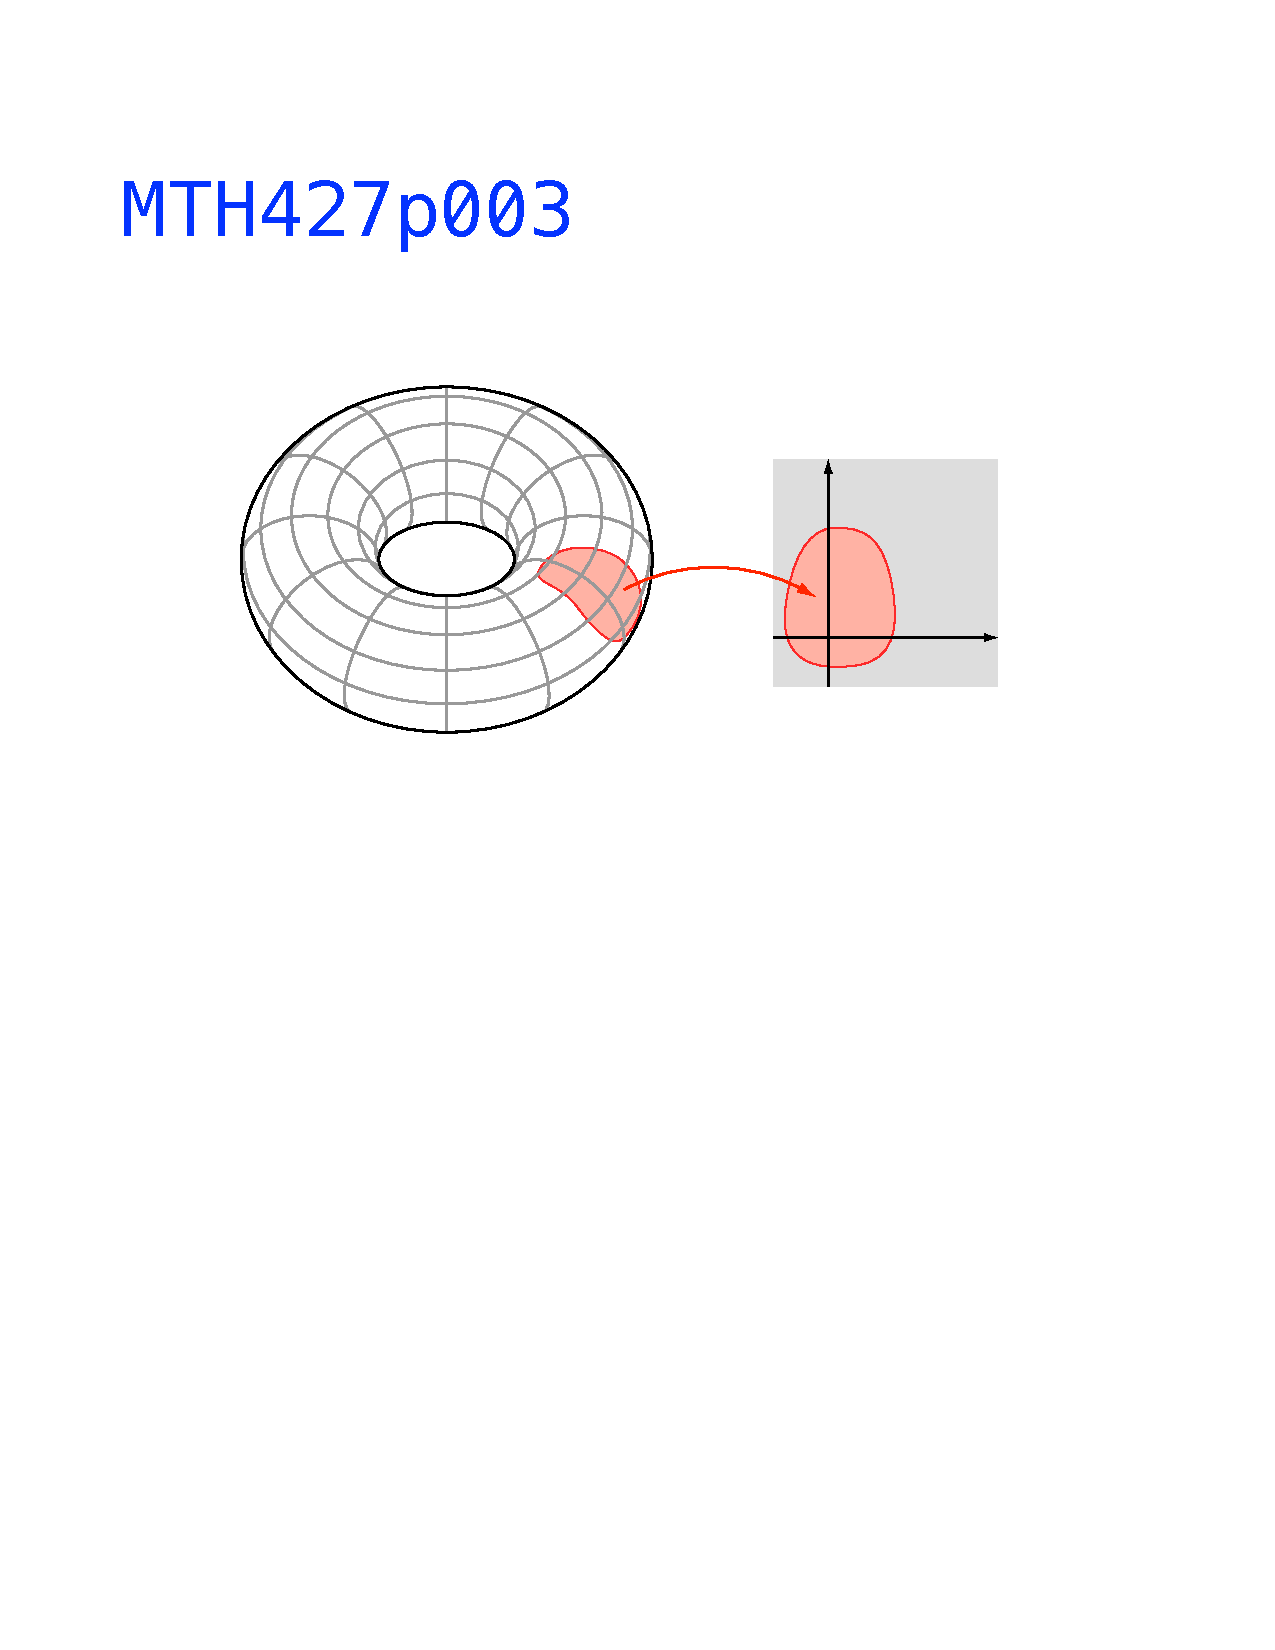
\includegraphics[width=\textwidth, trim=0mm 155mm 0mm 65mm, clip]{pictures/MTH427p003.pdf}}};


%%% COORDINATE GRID
%\draw[step=0.5, help lines] (0,0) to[grid with coordinates] (15,9);
%%% 

\node at (3.5,4){\small $M$};
\node at (7.85,2.1){\small $\color{red} U$};
\node at (9.3,2.4){\small $\varphi$};
\node at (11.1,2.2){\small $\color{red}V$};
x
\end{tikzpicture}
%---EBLANK


%---BBLANK  #\vfill
\begin{lemma}
\label{COORD LEMMA}
If $M$ is an $n$-dimensional manifold then:
\benu
\item for any point $x\in M$ there exists a coordinate chart $\varphi\colon U \to V$ such that $x\in U$, 
$V$ is an open ball $V= B(y, r)$, and $\varphi(x) = y$;
\item for any point $x\in M$ there exists a coordinate chart $\psi\colon U \to V$ such that $x\in U$,  
$V = \R^{n}$, and $\psi(x) = 0$.
\eenu
\end{lemma}

\begin{proof}
Exercise. 
\end{proof}
%---EBLANK

%---BBLANK #\newpage
\begin{example}
A space $M$ is a manifold of dimension $0$ if and only if $M$ is a countable (finite or infinite) discrete space.
\end{example}
%---EBLANK

%---BBLANK #\vskip 20mm
\begin{example}
If $U$ is an open set in $\R^{n}$ then $U$ is an $n$-dimensional manifold. The identity map 
$\id \colon U \to U$ is then  a coordinate chart defined on the whole manifold $U$. In particular 
$\R^{n}$ is an $n$-dimensional manifold. 
\end{example}
%---EBLANK

%---BBLANK #\vskip 20mm
\begin{example}
The $n$-dimensional sphere 
$$S^{n} := \{(x_{1}, \dots, x_{n+1})\in \R^{n+1} \ | \ x_{1}^{2}+\dots + x_{n+1}^{2} = 1 \}$$
is an $n$-dimensional manifold. 
%---EBLANK # \end{example}
Indeed, let $x = (x_{1}, \dots, x_{n+1}) \in S^{n}$. We need 
to show that there exists an open neighborhood of $x$ which is homeomorphic to an open subset 
of $\R^{n}$. Choose  $i\in \{1, 2, \dots, n+1\}$ such that $x_{i} \neq  0$. Assume that $x_{i} > 0$. Take 
$U_{i}^{+} = \{(y_{1}, \dots, y_{n+1})\in S^{n} \ | \ y_{i} >  0 \}$.
The set $U^{+}_{i}$ is open in $S^{n}$ and $x\in U^{+}_{i}$. We  have a continuous map 
$$h^{+}_{i}\colon U^{+}_{i} \to B(0, 1) \subseteq \R^{n}$$ 
given by $h(y_{1}, \dots, y_{n+1}) = (y_{1}, \dots, y_{i-1}, y_{i+1}, \dots, y_{n+1})$.  This map is 
a homeomorphism with the inverse $(h^{+}_{i})^{-1}\colon B(0,1) \to U^{+}_{i}$ given by 
$$(h^{+}_{i})^{-1}(t_{1}, \dots, t_{n}) = \left(t_{1}, \dots, t_{i-1}, \sqrt{1 - (t_{1}^{2} + \dots + t_{n}^{2})}, t_{i}, \dots t_{n},\right)$$
If $x_{i} <0$ then we can construct in a similar way a coordinate chart $h^{-}_{i}\colon U^{-}_{i}\to B(0, 1)$
where $U^{-}_{i} = \{(y_{1}, \dots, y_{n+1})\in S^{n} \ | \ y_{i} <  0 \}$.
\end{example}

%---BBLANK #\vskip 60mm
\begin{proposition}
\label{MANIFOLDPROD PROP}
If $M$ is an $m$-dimensional manifold and $N$ is an $n$-dimensional manifold then $M\times N$
is an $m+n$-dimensional manifold. 
\end{proposition}

\begin{proof}
Exercise. 
\end{proof}
%---EBLANK



\begin{example}
 The \emph{torus} is the space $T^{2} := S^{1}\times S^{1}$. Since $S^{1}$ is a manifold of dimension $1$, 
 thus by Proposition \ref{MANIFOLDPROD PROP} $T^{2}$ is a manifold of dimension $2$. Similarly, for 
 any $n\geq 2$ the \emph{$n$-dimensional torus}  $T^{n} := \prod_{i=1}^{n} S^{1}$ is a manifold of dimension $n$. 
\end{example}


%---BBLANK #\newpage
\begin{note}
There exist topological spaces that are locally homeomorphic to $\R^{n}$, 
but do not satisfy the the other conditions of the definition of a manifold (\ref{MANIFOLD DEF}). 
%---EBLANK # \end{note}
For example, the line with double origin is a topological space  $L$ defined as follows. As a set 
$L$ consist of all points of the real line $\R$ and one additional point that we will denote by $\tilde 0$: 

\begin{equation*}
\begin{tikzpicture}

\draw[ultra thick] (-2.5, 0) -- (2.5, 0) node[above = 1pt,  pos= 0.97] {\small $\R$};
\fill (0, 0) circle (0.1) node[below = 3pt]  {\small $0$};
\fill (0, 0.35) circle (0.1) node[above = 3pt]  {\small $\tilde 0$};

\end{tikzpicture}
\end{equation*}


A basis  $\BB$ of  the topology 
on $L$ consists of the following sets:
\benu
\item any open set in $\R$ is in $\BB$;  
\item for  any  $a<0$ and $b>0$ the set $(a, 0)\cup \{\tilde 0 \} \cup (0, b)$  is in $\BB$. 
\eenu
Notice that $L$ is locally homeomorphic to $\R$. Indeed, since $\R$ is an open set in $L$ thus any 
point of $L\ssmin \{\tilde 0\}$ has an open neighborhood homeomorphic to $\R$. Also, for any $a<0 < b$ the 
set $(a, 0)\cup \{\tilde 0 \}\cup (0, b)$ is an open neighborhood of $\tilde 0$ which is homeomorphic 
to the open interval $(a, b)$.  On the other hand $L$ is not a Hausdorff
space since the point $\tilde 0$ cannot be separated by open sets from $0\in \R$. 
Therefore $L$ is not a manifold.  There exist also spaces (e.g. Alexandroff long line) that  are locally homeomorphic to $\R^{n}$ and are Hausdorff, but are not second countable.  
\end{note}

The following theorem says that the dimension of a manifold is well defined:

%---BBLANK #\vskip 80mm
\begin{INVDIMTHM}
\label{INVDIM THM}
If $M$ is a non-empty topological space such that $M$ is a manifold of dimension $m$ and 
$M$ is also a manifold of dimension $n$ then $m=n$.
\end{INVDIMTHM}
%---EBLANK

In other words if a space is locally homeomorphic to $\R^{m}$ then if cannot be locally homeomorphic 
to $\R^{n}$ for  $n\neq m$. While this sounds obvious the proof for arbitrary $m$ and $n$ is actually 
quite involved and goes beyond the scope of this course. The proof is much simpler for $m=0$ and $m=1$  (exercise).

An slight generalization of the notion of a manifold is a manifold with boundary. 
Let $\HH^{n}$ denote the subspace of $\R^{n}$ given by 
$\HH^{n} = \{(x_{1}, \dots, x_{n})\in \R^{n} \ | \ x_{n} \geq 0 \}$. 

%---BBLANK #\newpage  \vspace*{50mm}
\begin{definition}
\label{MANIFOLD WITH BOUNDARY DEF}
A \emph{topological $n$-dimensional manifold with boundary} is a topological space $M$
which is a Hausdorff, second countable, and such that
every point of $M$ has an open neighborhood  homeomorphic to an 
open subset of $\HH^{n}$. 
\end{definition}
%---EBLANK

As before, if $M$ is a manifold with boundary, $U$ is an open set in $M$, $V$ is an open set in $\HH^{n}$
and $\varphi\colon U\to V$ is a homeomorphism then we say that $\varphi$ is a coordinate chart on $M$. 




\begin{nn}
Let $\partial \HH^{n} = \{ (x_{1}, \dots, x_{n})\in \HH^{n} \ | \ x_{n} = 0\}$.  If $M$ is an $n$-dimensional 
manifold with boundary,  $\varphi\colon U\to V$ is a coordinate chart, and $x\in U$ then 
there are two possibilities: 
\benu
\item $\varphi(x) \in \partial \HH^{n}$  
\item $\varphi(x) \not\in \partial \HH^{n}$
\eenu

%---BBLANK # \vskip 10mm
\begin{tikzpicture}

\node[anchor=south west,inner sep=0] at (0,0) 
{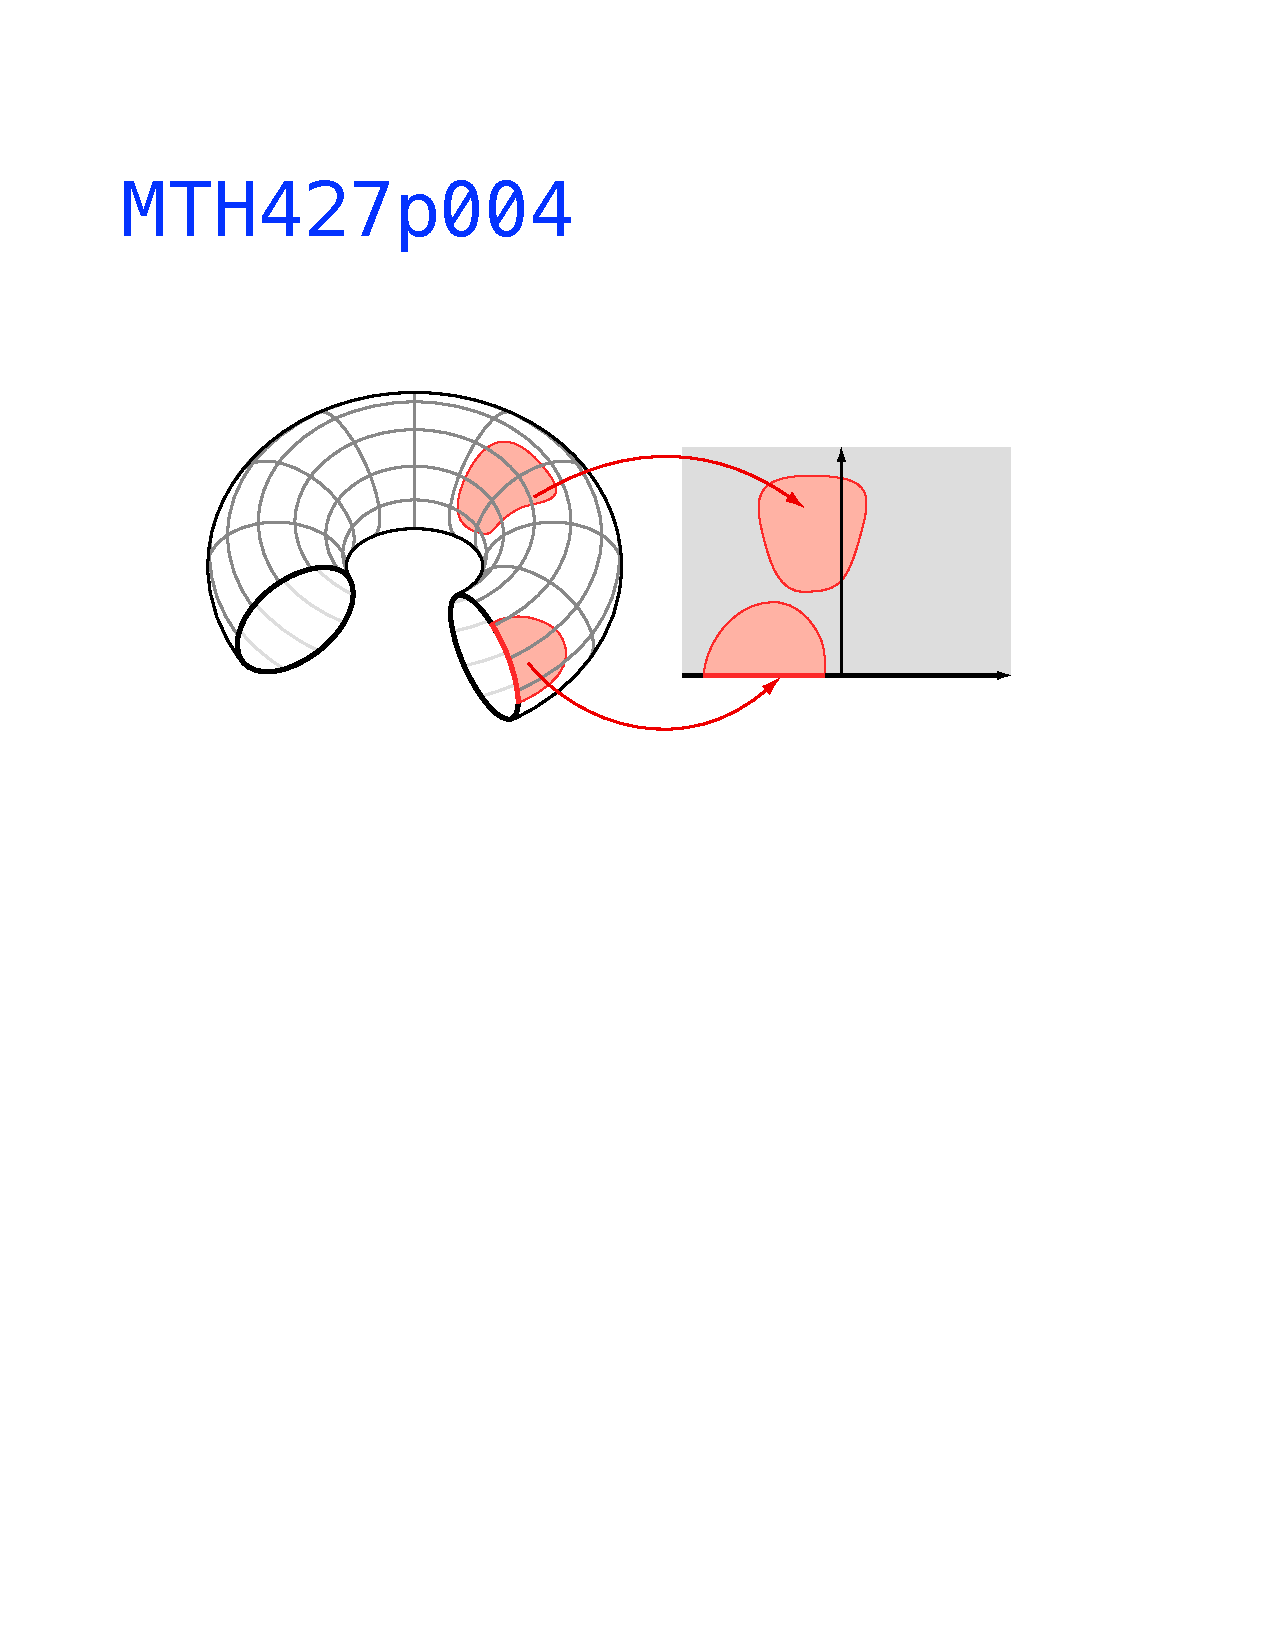
\includegraphics[width=\textwidth, trim=0mm 155mm 0mm 65mm, clip]{pictures/MTH427p004.pdf}};

%%% COORDINATE GRID
%\draw[step=0.5, help lines] (0,0) to[grid with coordinates] (15,9);
%%% 

\node at (3.4,4.2){\small $M$};
\node at (6.4,3.4){\small $\color{red} U_{1}$};
\node at (6.8,1.2){\small $\color{red} U_{2}$};
\node at (8.6,3.85){\small $\varphi_{1}$};
\node at (8.7,0.35){\small $\varphi_{2}$};
\node at (10.3,2.5){\small $\color{red}V_{1}$};
\node at (9.6,1.1){\small $\color{red}V_{2}$};
\node at (12.7,3.4){\small $\HH^{n}$};

\end{tikzpicture}
%---EBLANK 
In the first case we say that the point $x$ is a \emph{boundary point} of $M$, and in the
the second case that $x$ is an \emph{interior point} of $M$. 

The next theorem says that a point cannot be a boundary point and an interior point of $M$ at the same time:
\end{nn}


%---BBLANK # \vskip 30mm
\begin{theorem}
\label{INV BOUNDARY THM}
Let $M$ be an $n$-dimensional manifold with boundary, let $x_{0}\in M$ and  let $\varphi\colon U \to V$
be a local coordinate chart such that  $x_{0}\in U$. 
If $\varphi(x_{0}) \in \partial \HH^{n}$ then for any other local coordinate chart $\psi\colon U'\to V'$
such that $x_{0}\in U'$ we have $\psi(x_{0})\in \partial \HH^{n}$. 
\end{theorem}
%---EBLANK 

The proof in the general case requires similar machinery as the proof of Theorem \ref{INVDIM THM}, and so 
we will omit it here. The case when $n=1$ is much simpler (exercise). 

%---BBLANK # \vfill
\begin{definition}
 \index{boundary ! of a manifold@{$\sim$ of a manifold}}
Let $M$ be a manifold with boundary. The subspace of $M$ consisting of all boundary points of 
$M$ is called \emph{the boundary of $M$} and it is denoted by $\partial M$. 
\end{definition}
%---EBLANK 

%---BBLANK # \newpage
\begin{example}
The space $\HH^{n}$ is trivially an $n$-dimensional manifold with boundary. 
\end{example}
%---EBLANK 

%---BBLANK # \vskip 20mm
\begin{example}
\label{CLOSED BALL MFLD EXAMPLE}
For any $n$ the closed $n$-dimensional ball
$$\overline{B}^{n} = \{(x_{1}, \dots, x_{n})\in \R^{n} \ | \ x_{1}^{2}+\dots +x_{n}^{2} \leq 1\}$$
is an $n$-dimensional manifold with boundary (exercise). 
In this case we have $\partial \overline{B}^{n} = S^{n-1}$.  
\end{example}
%---EBLANK 

%---BBLANK # \vskip 50mm
\begin{example}
If $M$ is a manifold (without boundary) then we can consider  it as a manifold with boundary. 
where $\partial M = \varnothing$. 
\end{example}
%---EBLANK 

%---BBLANK # \vskip 30mm
\begin{example}
If $M$ is an $m$-dimensional manifold with boundary and $N$ is an $n$-dimensional manifold 
without boundary then $M\times N$ is an $(m+n)$-dimensional manifold with boundary (exercise). 
%---EBLANK  #\end{example}
In such case we have: $\partial (M\times N) = \partial M \times N$. For example the \emph{solid torus} 
$\overline{B}^{2}\times S^{1}$ is a $3$-dimensional manifold with boundary, and 
$\partial (\overline{B}^{2}\times S^{1}) = S^{1}\times S^{1} = T^{2}$.   

Even more generally, if $M$ is an $m$-dimensional manifold with boundary and $N$ is 
an $n$-dimensional manifold with boundary then $M\times N$ is  an $(m+n)$-dimensional manifold 
with boundary and $\partial (M\times N) = (\partial M \times N) \cup (M \times \partial N)$ (exercise). 
\end{example}



\begin{proposition}
\label{BOUNDARY INT SUBMANIFOLD PROP}
If $M$ is an $n$-dimensional manifold with boundary then:
\benu
\item $M\ssmin \partial M$ is an open subset of $M$ and it is an $n$-dimensional manifold (without boundary); 
\item $\partial M$ is a closed subset of $M$ and it is an $(n-1)$-dimensional manifold (without boundary). 
\eenu 
\end{proposition}

\begin{proof}
Exercise. 
\end{proof}



%---BBLANK # \newpage
\begin{theorem}
\label{MANIFOLD METRIZATION THM}
Every topological manifold (with or without boundary) is metrizable. 
\end{theorem}
%---EBLANK 

Our argument  will use the following fact, the proof of which will be postponed until later 
(see Exercise \ref{MFLD LOCAL CLOSED BALL EXERCISE}).

%---BBLANK # \vskip 10mm
\begin{lemma}
\label{MFLD LOCAL CLOSED BALL LEMMA}
Let $M$ be an $n$-dimensional topological manifold, and let $\varphi\colon U \to V$ be a coordinate 
chart on $M$. If $\xov{B}(x, r)$ is a closed ball in $\R^{n}$ such that $\xov{B}(x, r) \subseteq V$ then 
the set $\varphi^{-1}(\xov{B}(x, r))$ is  closed in $M$. 
\end{lemma}
%---EBLANK 

\begin{proof}[Proof of Theorem \ref{MANIFOLD METRIZATION THM}]
We will use Urysohn Metrization Theorem \ref{REGULAR URYSOHN METR THM}. Since by definition 
every manifold is second countable it will be enough to prove that manifolds are regular topological spaces. 

Let $M$ be an $n$-dimensional manifold, let $A\subseteq M$ be a closed set, and let $x\in M$ be a point 
such that $x\not\in A$.  We need to show that there exists open sets $W, W'\subseteq M$ such that 
$A\subseteq W$, $x\in W'$ and $W\cap W' = \varnothing$.  Assume first that $x$ does not belong to the boundary of $M$.  We can find an open neighborhood $U$ of $x$ and homeomorphism 
$\varphi \colon U \to \R^{n}$ such that $\varphi(x) = 0$. 
Since $A$ is closed in $M$ the set $A\cap U$ is closed in $U$, and so 
$\varphi(A\cap U)$ is closed in $\R^{n}$. Therefore the set $\R^{n}\ssmin\varphi(A\cap U)$ is open 
in $\R^{n}$. Since $0 = \varphi(x)\in \R^{n}\ssmin\varphi(A\cap U)$ we can find an open ball 
$B(0, \varepsilon)$ such that $B(0, \varepsilon) \subseteq \R^{n}\ssmin\varphi(A\cap U)$:


%---BBLANK # \vskip 60mm
\begin{tikzpicture}
\node[anchor=south west,inner sep=0] at (0,0) 
{{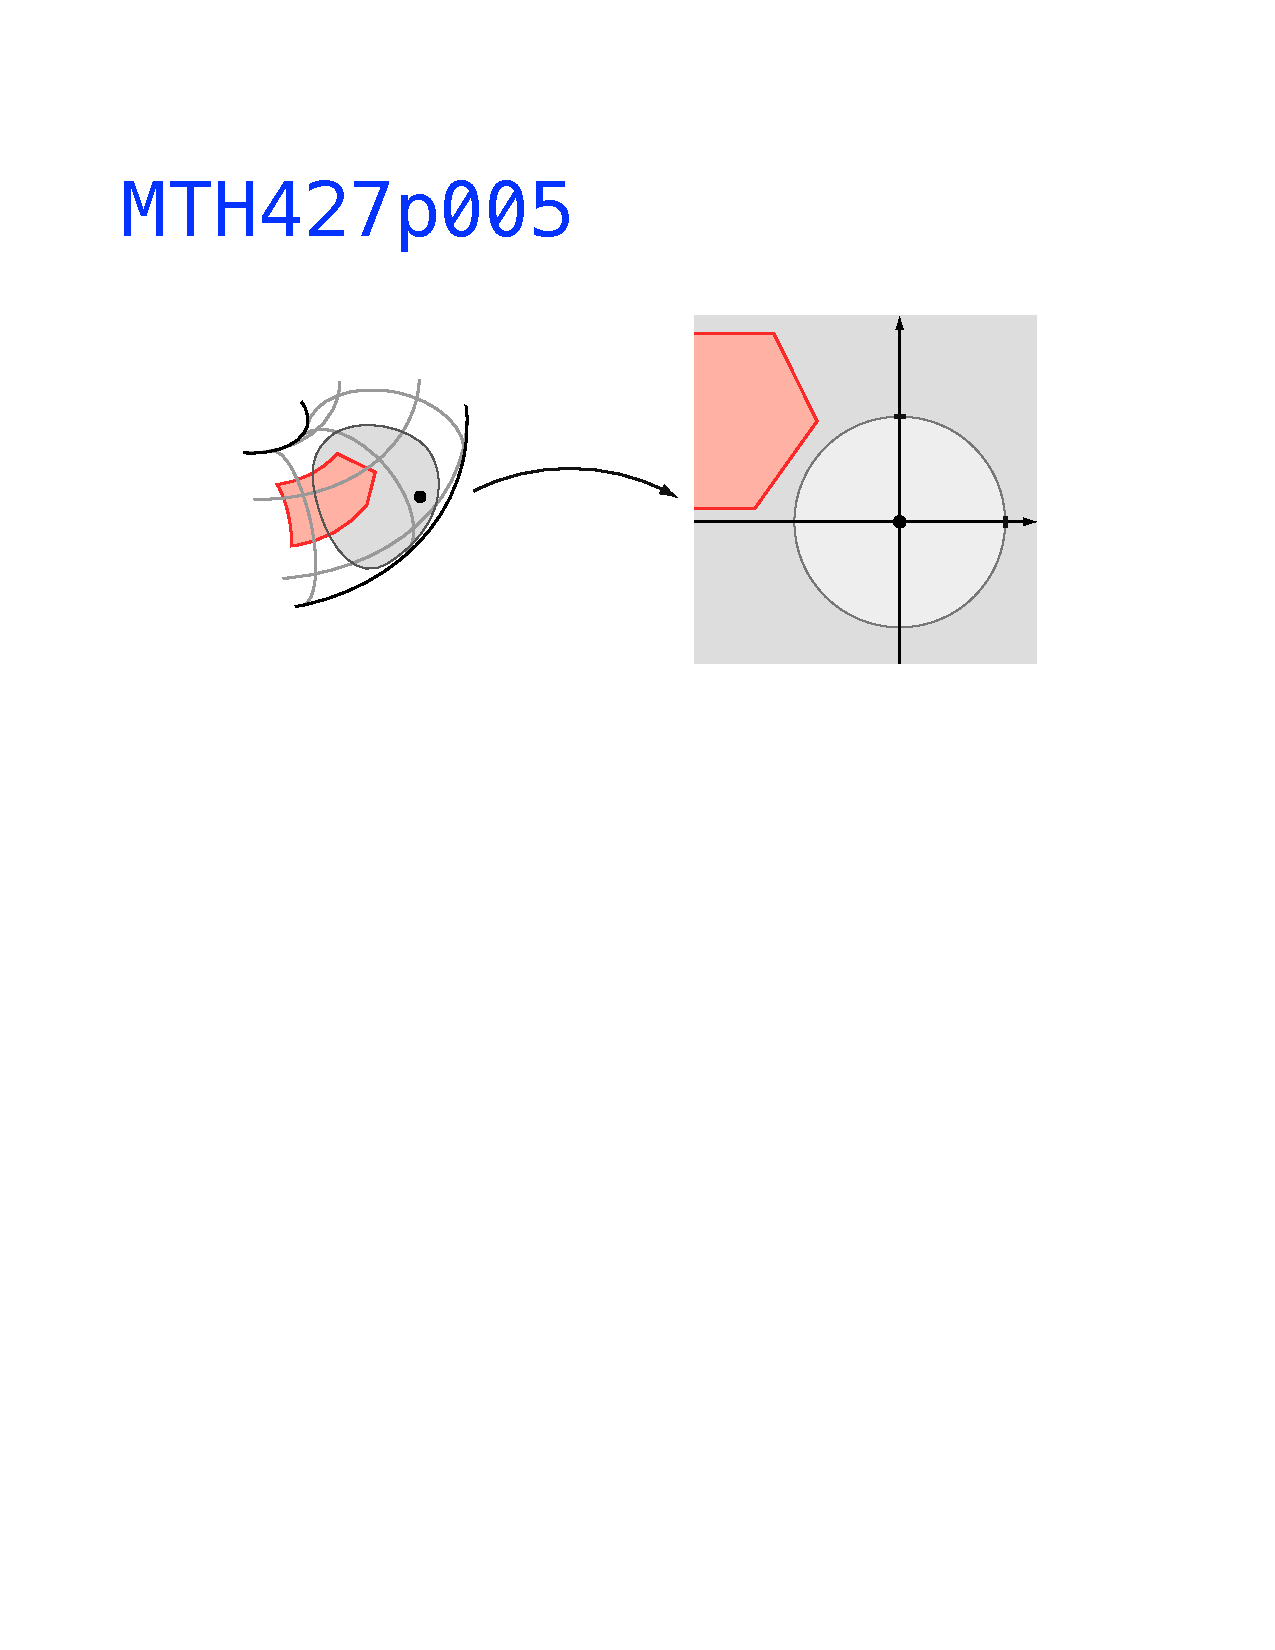
\includegraphics[width=\textwidth, trim=0mm 163mm 0mm 50mm, clip]{pictures/MTH427p005.pdf}}};

%%% COORDINATE GRID
%\draw[step=0.5, help lines] (0,0) to[grid with coordinates] (15,9);
%%% 

\node at (3.8,4.3){\small $M$};
\node at (4.4,2.5){\small $\color{red} A$};
\node at (4.9,1.8){\small $U$};
\node at (5.48,2.7){\small $x$};
\node at (7.5,3.1){\small $\varphi$};
\node at (9.75,3.47){\small $\color{red}\varphi(A\cap U)$};
\node at (12.1,2.45){\small $\varphi(x)$};
\node at (13.15,1.95){\small $\varepsilon$};
\node at (11.85,3.65){\small $\varepsilon$};
\node at (13.1,4.5){\small $\R^{n}$};

\end{tikzpicture}
%---EBLANK 

 
Take $W = M \ssmin \varphi^{-1}(\xov{B}(0, \frac{\varepsilon}{2}))$ and 
$W' = \varphi^{-1}(B(0, \frac{\varepsilon}{2}))$. Notice that $x\in W'$. Also, since $W'$ is open in 
$U$ and $U$ is open in $M$ we obtain that $W'$ is open in $M$. Next, by Lemma 
\ref{MFLD LOCAL CLOSED BALL LEMMA} the set $\varphi^{-1}(\xov{B}(0, \frac{\varepsilon}{2}))$
is closed in $M$, so $W$ is open in $M$. Moreover, since 
$W' \subseteq \varphi^{-1}(\xov{B}(0, \frac{\varepsilon}{2}))$ we obtain that $W\cap W' = \varnothing$. 
It remains to show that $A\subseteq W$, or equivalently that 
$A\cap \varphi^{-1}(\xov{B}(0, \frac{\varepsilon}{2})) = \varnothing$. If $y\in A$ and $y\not \in U$ then 
$y\not\in \varphi^{-1}(\xov{B}(0, \frac{\varepsilon}{2}))$ since $\varphi^{-1}(\xov{B}(0, \frac{\varepsilon}{2}))
\subseteq U$. Also, if $y\in A\cap U$ then $y\not\in \varphi^{-1}(\xov{B}(0, \frac{\varepsilon}{2}))$ by the 
choice of $\varepsilon$, and so we are done. In case when $x\in \partial M$ we can use a similar argument. 
 


\end{proof}





%%%%%%%%%%%%%%%%%%%%%%%%%%%%%%%
%  EXERCISES
%%%%%%%%%%%%%%%%%%%%%%%%%%%%%%%

\exercises

%\begin{exercise}
%Let $D$ be the 'donut' subspace of $\R^{3}$ given by:
%$$D = \left\{(x_{1}, x_{2}, x_{3})\in \R^{3} \ \left| 
%\ \left(2-\sqrt{x_{1}^{2}+{x_{2}^{2}}}\right)^{2} + x_{3}^{2} =1\right. \right\}$$
%Show that $D$ is homeomorphic to the torus $T^{2} = S^{1}\times S^{1}$.
%\end{exercise}

\begin{exercise}
Prove Lemma \ref{COORD LEMMA}.
\end{exercise}




\begin{exercise}
\label{SMALL COORD NBHD EXERCISE}
Let $M$ be an $n$-dimensional manifold, let $x_{0}\in M$ and let $W\subseteq M$
be an open set such that $x_{0}\in W$. Show that there exists a coordinate neighborhood 
$U\subseteq M$ such that $x_{0}\in U$ and $U\subseteq W$.  
\end{exercise}





\begin{exercise}
The goal of this exercise is to prove the Invariance of Dimension Theorem \ref{INVDIM THM}
in small dimensions. 

a)  Let $M$ be a manifold of dimension $0$. Show that $M$  is not locally homeomorphic
to $\R^{n}$ for any $n\neq 0$. 

b) Let $M$ be a manifold of dimension $1$. Show that $M$ is not locally homeomorphic
to $\R^{n}$ for any $n\neq 1$. 
\end{exercise}





\begin{exercise}
Prove Theorem \ref{INV BOUNDARY THM} in the case when $M$ is a $1$-dimensional 
manifold with boundary. 
\end{exercise}





\begin{exercise}
Let $M$ be an $m$-dimensional manifold with boundary and $N$ 
an $n$-dimensional manifold with boundary Show that $M\times N$ is  an $(m+n)$-dimensional manifold 
with boundary and $\partial (M\times N) = (\partial M \times N) \cup (M \times \partial N)$ 
\end{exercise}



\begin{exercise}
Prove Proposition \ref{BOUNDARY INT SUBMANIFOLD PROP}. 
\end{exercise}





\newpage
%%%%%%%%%%%%%%%%%%%%%%%%%%%%%%%
%%%%%%%%%%%%%%%%%%%%%%%%%%%%%%%
%%%
%%%  COMPACT SPACES
%%%
%%%%%%%%%%%%%%%%%%%%%%%%%%%%%%%
%%%%%%%%%%%%%%%%%%%%%%%%%%%%%%%


%---BBLANK
\chapter{Compact Spaces}
%---EBLANK
\chaptermark{Compact Spaces}

\thispagestyle{firststyle}
 
% \emph{
% \begin{tabular}{@{}l@{}}
%An old scholar confessed he's got whacked \\ 
%When he set to write down each known fact. \\
%I, lamented the the sage,\\
%Covered many a page  \\
%But my knowledge in so non-compact!
%\end{tabular}
%}
 

 %---BBLANK
\begin{definition}
\label{COVER DEF}
Let $X$ be a topological space.  A \emph{cover} of $X$ is a collection $\mathcal{Y} = \{Y_{i}\}_{i\in I}$
of subsets of $X$ such that $\bigcup_{i\in I} Y_{i} = X$.

\begin{equation*}
\begin{tikzpicture}[scale=0.8]
\begin{scope}
\begin{scope}
\clip (-0.5,0.5) rectangle (5, 3.5);
\fill[mypink, opacity = 0.6] (0.7, 2) circle [radius = 2.5];
\fill[mypink, opacity = 0.6] (4, 4) circle [radius = 2.5];
\fill[mypink, opacity = 0.6] (3.3, .5) circle [radius = 2.2];
\draw[red] (0.7, 2) circle [radius = 2.5];
\draw[red](4, 4) circle [radius = 2.5];
\draw[red] (3.3, .5) circle [radius = 2.2];
\end{scope}
\draw (-0.5,0.5) rectangle (5,3.5);
\node[anchor=west] at (-0.4 , 3) { \small $X$};
\node[anchor=west] at (-0.4 , 1) { \small \color{red} $Y_{1}$};
\node[anchor=east] at (4.9 , 1) { \small \color{red} $Y_{2}$};
\node[anchor=east] at (4.9 , 3) { \small \color{red} $Y_{3}$};
\end{scope}
\end{tikzpicture}
\end{equation*}

If the sets $Y_{i}$ are open in $X$ for all $i\in I$ then $\mathcal{Y}$ is an \emph{open cover} of $X$. 
If $\mathcal{Y}$ consists of finitely many sets then $\mathcal{Y}$ is a \emph{finite cover} of $X$.   

\end{definition}  
%---EBLANK

 %---BBLANK #\vskip 20mm
\begin{definition}
Let $\mathcal{Y} = \{Y_{i}\}_{i\in I}$ be a cover of $X$. A \emph{subcover} of $\mathcal{Y}$ is 
cover $\mathcal{Y}'$ of $X$ such that every element of $\mathcal{Y}'$ is in $\mathcal{Y}$. 
\end{definition}
%---EBLANK

\begin{example}
Let $X = \R$. The collection 
$$\YY = \{(m, n)\subseteq \R \ | \ m, n\in \Z, \ m< n \}$$
is an open cover of $\R$, and the collection 
$$\YY' = \{(-n, n) \subseteq \R\ | \ n= 1, 2, \dots  \}$$
is a subcover of $\YY$.  
\end{example}

 %---BBLANK # \vfill
\begin{definition}
\index{space! compact@{compact $\sim$}}
A space $X$ is \emph{compact} if every open cover of $X$ contains a finite subcover. 
\end{definition}
%---EBLANK 

 %---BBLANK # \newpage
\begin{example}
A discrete topological space $X$ is compact if and only if  $X$ consists of finitely many points. 
\end{example}
%---EBLANK 


 %---BBLANK # \vskip 50mm
\begin{example}
Let $X$ be a subspace of $\R$ given by 
$$X = \{0 \} \cup \{\ \tfrac{1}{n} \ | \ n= 1, 2, \dots \}$$
The space $X$ is compact. 
%---EBLANK # \end{example}
Indeed, let $\UU = \{ U_{i} \}_{i\in I}$ be any open cover of $X$
and let $0\in U_{0}$. Then there exists $N>0$ such that $\frac{1}{n}\in U_{i_{0}}$ for all $n> N$. 
For $n=1, \dots, N$ let $U_{i_{n}}\in \UU$ be a set such that $\frac{1}{n}\in U_{i_{n}}$. We have:
$$X = U_{i_{0}} \cup U_{i_{1}} \cup \dots \cup U_{i_{N}}$$
so $\{U_{i_{0}}, U_{i_{1}}, \dots, U_{i_{N}}\}$ is a finite subcover of $\UU$.
\end{example}


 %---BBLANK # \vskip 50mm
\begin{example}
The real line $\R$ is not compact
%---EBLANK #\end{example}
since the open cover 
$$\YY = \{(n-1, n+1) \subseteq \R \ | \ n\in \Z \}$$
does not have any finite subcover. 
\end{example}




%---BBLANK # \newpage \vspace*{-25mm}
\begin{proposition}
\label{CLOSEDINT COMPACT PROP}
For any $a< b$ the closed interval $[a, b]\subseteq \R$ is compact.  
\end{proposition}
%---EBLANK 

\begin{proof}
Let $\UU$ be an open cover of $[a, b]$ and let 
$$A = \{x\in [a, b] \ | \  \text{the interval $[a, x]$ can be covered by a finite number of elements of $\UU$}\}$$
Let $x_{0} := \sup A$. 

\emph{Step 1.} We will show that $x_{0} > a$. Indeed, let $U\in \UU$ be a set such that $a\in U$. 
Since $U$ is open we have $[a, a+\varepsilon ) \subseteq U$ for some $\varepsilon > 0$. It follows 
that $x\in A$ for all $x\in [a, a+\varepsilon)$. Therefore $x_{0}\geq a+\varepsilon$. 


\emph{Step 2.} Next, we  will show  that $x_{0}\in A$. Let $U_{0}\in \UU$ be a set such that 
$x_{0}\in U_{0}$. Since $U_{0}$ is open and $x_{0}> a$ there exists $\varepsilon _{1} >0$ such that
$(x_{0}-\varepsilon_{1} , x_{0}] \subseteq U_{0}$. Also, since $x_{0} = \sup A$  there is $x\in A$
such that $x\in (x_{0}-\varepsilon_{1} , x_{0}]$. Notice that  
$$[a, x_{0}] = [a, x]\cup (x_{0}-\varepsilon_{1}, x_{0}]$$
By assumption the interval $[a, x]$ can be covered by a finite number of sets from  $\UU$ and 
$(x_{0}-\varepsilon_{1}, x_{0}]$ is covered by $U_{0}\in \UU$. As a consequence $[a, x_{0}]$
can be covered by a finite number of elements of $\UU$, and so $x_{0}\in A$. 

\emph{Step 3.} In view of Step 2 it suffices to show  that $x_{0} = b$.  To see this take again 
$U_{0}\in \UU$ to be a set such that $x_{0}\in \UU$. If $x_{0}< b$ then there exists $\varepsilon_{2} >0$
such that $[x_{0}, x_{0}+\varepsilon_{2} ) \subseteq U_{0}$. Notice that for any  
$x\in (x_{0}, x_{0}+\varepsilon_{2})$ the interval $[a, x]$ can be covered by a finite number of elements of 
$\UU$, and thus $x\in A$. Since $x> x_{0}$ this contradicts the assumption that $x_{0} = \sup A$.  

\end{proof}


%---BBLANK # \newpage
\begin{proposition}
\label{COMPACT ONTO PROP}
Let $f\colon X\to Y$ be a continuous function. If  $X$ is compact and $f$ is onto then $Y$ is compact. 
\end{proposition}

\begin{proof}
Exercise.
%If $\{U_{i}\}_{i \in I}$ be an open cover of $Y$ then $\{ f^{-1}(U_{i}) \}_{i\in I}$ is an open cover 
%of $X$. Since $X$ is compact we can find a finite subcover $\{f^{-1}(U_{i_{1}}), \dots, f^{-1}(U_{i_{n}})\}$. 
%We have:
%\begin{align*}
%U_{i_{1}} \cup \dots \cup U_{i_{n}} = & \\
%f(f^{-1}(U_{i_{1}})) \cup \dots \cup f(f^{-1}(U_{i_{n}})) = & \\
%f(f^{-1}(U_{i_{1}}), \dots, f^{-1}(U_{i_{n}})) =  & 
%\ f(X) =  Y \\
%\end{align*} 
%Thus $\{U_{1}, \dots, U_{n}\}$ is a finite subcover of $X$. 
\end{proof}
%---EBLANK 


%---BBLANK # \vskip 30mm
\begin{corollary}
\label{COMPACT IMAGE COR}
Let $f\colon X\to Y$ be a continuous function. If  $A\subseteq X$ is compact  then $f(A)\subseteq Y$ is compact. 
\end{corollary}
%---EBLANK 

\begin{proof}
The function $f|_{A}\colon A \to f(A)$ is onto, so this follows from Proposition \ref{COMPACT ONTO PROP}.
\end{proof}

%---BBLANK # \vskip 70mm
\begin{corollary}
\label{COMP TOP INV PROP}
Let $X$, $Y$ be topological spaces.
If $X$ is  compact  and $Y \cong X$ then $Y$ is compact. 
\end{corollary}
%---EBLANK 

\begin{proof}
Follows from Proposition \ref{COMPACT ONTO PROP}.
\end{proof}


\begin{example}
For any $a< b$ the open interval $(a, b)\subseteq \R$ is not compact since $(a, b)\cong \R$. 
\end{example}



%---BBLANK # \newpage
\begin{proposition}
\label{CLOSED SUBSP OF COMPACT PROP}
Let $X$ be a compact space. If $Y$ is a closed subspace of $X$ then $Y$ is compact. 
\end{proposition}


\begin{proof}
Exercise.
%Let $\{U_{i}\}_{i\in I}$ be an open cover of $Y$. For each $i\in I$ let $V_{i}$ be an open set 
%in $X$ such that $V_{i}\cap Y = U_{i}$. Also let $W = X\ssmin Y$. Notice that 
%$$\bigcup_{i\in I} V_{i} \cup W \supseteq Y \cup W = X$$
%so the collection $\{V_{i}\}_{\in I} \cup \{W\}$ is an open cover of $X$. Since $X$ is a compact space 
%this cover has a finite subcover $\{V_{i_{1}}, \dots, V_{i_{n}}, W\}$ for some $i_{1}, \dots, i_{n}\in I$. 
%It follows that the collection $\{U_{i_{1}}, \dots, U_{i_{1}}\}$ is a finite subcover of $\{U_{i}\}_{i\in I}$.
\end{proof}
%---EBLANK 

%---BBLANK # \vskip 10mm
\begin{proposition}
\label{COMPACT SUBSPACE PROP}
Let $X$ be a  Hausdorff space and let  $Y\subseteq X$. If $Y$ is compact then it is closed in $X$. 
\end{proposition}
%---EBLANK 


Proposition \ref{COMPACT SUBSPACE PROP} is a direct consequence of the following fact: 

%---BBLANK # \vskip 10mm
\begin{lemma}
\label{COMPACT SET SEPARATION LEMMA}
Let $X$ be a Hausdorff space, let $Y\subseteq X$ be a compact subspace, and let $x\in X \ssmin Y$. 
There exists open sets $U, V\subseteq X$ such that $x\in U$, $Y\subseteq V$ and $U\cap V = \varnothing$. 

\begin{equation*}
\begin{tikzpicture}
\draw (0,0) rectangle (5, 3);
\fill[mypink, opacity = 0.8] (1.4, 1.5) circle (0.7);
\fill (1.4, 1.5) circle (0.07) node[below = 1pt] {\small $x$};
\draw[red] (1.4, 1.5) circle (0.7);
\fill[mypink, rounded corners, opacity=0.8] (2.7, 0.3) rectangle (4.6, 2.7); 
\draw[red, rounded corners] (2.7, 0.3) rectangle (4.6, 2.7); 
\draw[ultra thick, fill = mygray3] (3.2, 0.8) rectangle (4.1, 2.2) node[pos = 0.5] {\small $Y$}; 
\node at (1.2 , 1.9) {\small \color{red} $U$};
\node at (4.3 , 2.4) {\small \color{red} $V$};
\node at (0.4 , 2.6) {\small  $X$};
\end{tikzpicture}
\end{equation*} 

\end{lemma}
%---EBLANK 



\begin{proof} 
Since $X$ is a Hausdorff space for any point $y\in Y$ there exist open sets
$U_{y}$ and $V_{y}$ such that $x\in U_{y}$, $y\in V_{y}$ and 
$U_{y}\cap V_{y} = \varnothing$. Notice that $Y\subseteq \bigcup_{y\in Y} V_{y}$. 
Since $Y$ is compact we can find a finite number of points $y_{1}, \dots, y_{n}\in Y$ such that 
$$Y\subseteq V_{y_{1}}\cup \dots \cup V_{y_{n}}$$
Take $V = V_{y_{1}}\cup \dots \cup V_{y_{n}}$ and $U := U_{y_{1}}\cap \dots \cap U_{y_{n}}$.

%%%%%%%%%%
% TO BE FINISHED
%%%%%%%%%%
\begin{equation*}
\begin{tikzpicture}
\draw (-0.5,-0.4) rectangle (5, 3.35);

\fill[mygray3] (2.8, 0.55) rectangle (4.7, 2.5); 

\fill[mygray3, rounded corners = 9pt, opacity=0.6] (-0.2, 0.0) rectangle (1.7, 2.3); 
\fill[mygray3, rounded corners = 9pt, opacity=0.6] (0.5, 1.5) rectangle (2.5, 2.95); 
\fill[mypink, rounded corners = 9pt, opacity=0.6] (2.0, 1.7) rectangle (3.8, 3.15); 
\fill[mypink, rounded corners = 9pt, opacity=0.6] (1.0, -0.2) rectangle (3.8, 1.3); 

\draw[ultra thick] (2.8, 0.55) rectangle (4.7, 2.5); 

\draw[rounded corners = 9pt] (-0.2, 0.0) rectangle (1.7, 2.3); 
\draw[rounded corners = 9pt] (0.5, 1.5) rectangle (2.5, 2.95); 
\draw[red, rounded corners = 9pt] (2.0, 1.7) rectangle (3.8, 3.15); 
\draw[red, rounded corners = 9pt] (1.0, -0.2) rectangle (3.8, 1.3); 

\fill (1.2, 2.0) circle (0.07) node[left = 1pt] {\small $x$};
\fill (3.1, 2.0) circle (0.07) node[right = 1pt] {\small $y_{1}$};
\fill (3.1, 1.0) circle (0.07) node[right = 1pt] {\small $y_{2}$};

\node at (-0.1 , 2.95) {\small  $X$};
\node at (4.35 , 2.2) {\small  $Y$};
\node[red] at (3.45, 2.8) {\small $V_{y_{1}}$};
\node[red] at (3.45, 0.2) {\small $V_{y_{2}}$};
\node at (0.25, 0.3) {\small $U_{y_{1}}$};
\node at (0.9, 2.6) {\small $U_{y_{2}}$};
\end{tikzpicture}
\end{equation*} 
\end{proof}

\begin{proof}[Proof of Proposition \ref{COMPACT SUBSPACE PROP}]
By Lemma \ref{COMPACT SET SEPARATION LEMMA} for each point $x\in X \ssmin Y$ we 
can find an open set $U_{x}\subseteq X$ such that $x\in U_{x}$ and $U_{x}\subseteq X\ssmin Y$. 
Therefore $X \ssmin Y$ is open and so $Y$ is closed. 
\end{proof}

%---BBLANK  # \newpage
\begin{corollary}
Let $X$ be a  compact Hausdorff space. A subspace  
$Y\subseteq X$ is compact if and only if   $Y$ is closed in $X$. 
\end{corollary}
%---EBLANK

\begin{proof}
Follows from Proposition \ref{CLOSED SUBSP OF COMPACT PROP} and 
Proposition \ref{COMPACT SUBSPACE PROP}.
\end{proof}

%---BBLANK  # \vskip 20mm
\begin{proposition}
\label{COMPACT TO HAUSDORFF CLOSED MAP PROP}
Let $f\colon X\to Y$ be a continuous function, where $X$ is a compact space and $Y$ is a Hausdorff space. 
For any closed set $A\subseteq X$ the set $f(A)$ is closed in $Y$.  
\end{proposition}
%---EBLANK


\begin{proof}
Let $A\subseteq X$ be a closed set. By Proposition \ref{CLOSED SUBSP OF COMPACT PROP}
$A$ is  a compact space and thus by Corollary  \ref{COMPACT IMAGE COR}  $f(A)$ is  a 
compact   subspace of $Y$. Since $Y$ is a Hausdorff space, 
using Proposition \ref{COMPACT SUBSPACE PROP} we obtain that $f(A)$ is closed in $Y$. 
\end{proof}


%---BBLANK  # \vskip 50mm
\begin{proposition}
\label{COMPACT TO HAUSDORF BIJ PROP}
Let $f\colon X\to Y$ be a continuous bijection. If $X$ is a compact space and $Y$ is a Hausdorff 
space then $f$ is a homeomorphism. 
\end{proposition}
%---EBLANK

\begin{proof}
This follows from  Proposition \ref{HOMEO OPEN PROP} and Proposition \ref{COMPACT TO HAUSDORF BIJ PROP}. 
\end{proof}


%---BBLANK  # \newpage
\begin{theorem}
\label{COMPACT IS NORMAL THM}
If $X$ is a  compact Hausdorff space then $X$ is normal.  
\end{theorem}
%---EBLANK

\begin{proof}
\emph{Step 1.} We will show first that $X$ is a regular space (\ref{REGULAR DEF}). 
Let $A\subseteq X$ be  a closed  set and let $x\in X\ssmin A$. We need to show that 
there exists open sets $U, V\subseteq X$ such that $x\in U$, $A\subseteq V$ and 
$U\cap V = \varnothing$. Notice that by Proposition \ref{CLOSED SUBSP OF COMPACT PROP}
the set $A$ is compact. Since $X$ is Hausdorff existence of the sets $U$ and $V$ follows from 
Lemma \ref{COMPACT SET SEPARATION LEMMA}. 


\emph{Step 2.} Next, we show that $X$ is normal. Let $A, B\subseteq X$ be closed sets such that 
$A\cap B = \varnothing$.  
By Step 1 for every $x\in A$ we can find open sets $U_{x}$ and $V_{x}$ such that $x\in U_{x}$, 
$B\subseteq V_{x}$ and $U_{x}\cap V_{x} = \varnothing$. The collection $\UU = \{U_{x}\}_{x\in A}$ 
is an open cover of $A$. Since $A$ is compact there is a 
finite number of points $x_{1}, \dots, x_{m}\in A$ such that $\{U_{x_{1}}, \dots, U_{x_{m}}\}$
is a cover of $A$. Take $U := \bigcup_{i=1}^{m} U_{x_{i}}$ and $V := \bigcap_{i=1}^{m}V_{x_{i}}$.
Then $U$ and $V$ are open sets, $A\subseteq U$, $B \subseteq V$ and $U\cap V = \varnothing$. 
\end{proof}




\ 

%%%%%%%%%%%%%%%%%%%%%%%%%%%%%%%
%  EXERCISES
%%%%%%%%%%%%%%%%%%%%%%%%%%%%%%%

\exercises


\begin{exercise}
Prove Proposition \ref{COMPACT ONTO PROP}.
\end{exercise}




\begin{exercise}
Prove Proposition \ref{CLOSED SUBSP OF COMPACT PROP}.
\end{exercise}



\begin{exercise}
\label{COMPACT IN HAUSDORFF EXERCISE}
Let $X$ be a Hausdorff space and let $A\subseteq X$. Show that the following conditions are equivalent:
\benu
\item[(i))] $A$ is compact
\item[(ii))] $A$ is closed in $X$ and in any open cover $\{U_{i}\}_{i\in I}$ of $X$ there exists a finite number 
of sets $U_{i_{1}}, \dots, U_{i_{n}}$ such that $A \subseteq \bigcup_{k=1}^{n} U_{i_{k}}$. 
\eenu
\end{exercise}




\begin{exercise}
a) Let $X$ be a compact  space and for $i=1, 2, \dots$ let $A_{i} \subseteq X$ be a 
non-empty closed set. Show that if $A_{i+1} \subseteq A_{i}$ for all $i$
then $\bigcap_{i=1}^{\infty}A_{i} \neq \varnothing$. 

b) Give an example of a (non-compact) space $X$ and  closed non-empty sets 
$A_{i}\subseteq X$ satisfying $A_{i+1}\subseteq A_{i}$ for $i=1, 2, \dots$ such that 
$\bigcap_{i=1}^{\infty} A_{i} = \varnothing$. 
\end{exercise}




\begin{exercise} a) Let $X$ be a compact  Hausdorff space and for $i=1, 2, \dots$ let $A_{i} \subseteq X$ be a 
closed, connected set. Show that if $A_{i+1} \subseteq A_{i}$ for all $i$
then $\bigcap_{i=1}^{\infty}A_{i}$ is connected. 

b) Give an example of a space $X$ and  subspaces $A_{1}\supseteq A_{2}\supseteq {\dots}$
such that $A_{i}$ is connected and closed in $X$ for each $i$, but $\bigcap_{i=1}^{\infty}A_{i}$ is not connected.
\end{exercise}






\begin{exercise}
\label{COMP MINMAX EXE}
The goal of this exercise is to show that if $f\colon X\to \R$ is a continuous function 
and $X$ is a compact space then there exist points $x_{1}, x_{2}\in X$ such that 
$f(x_{1})$ is the minimum value of $f$ and $f(x_{2})$ is the maximum value. 

Let $X$ be a compact space and let $f\colon X\to \R$ be a continuous function. 

a) Show that there exists $C > 0 $  such that $|f(x)| < C$ for all 
$x\in X$. 

b) By part a)  there exists $C> 0$ such that $f(X)\subseteq [-C, C]$. This implies  that $\inf f(X)\neq -\infty$
and $\sup f(X)\neq +\infty$. Show that there are points $x_{1}, x_{2}\in X$ such that 
$f(x_{1}) = \inf f(X)$ and  that $f(x_{2}) = \sup f(X)$. 
\end{exercise}




\begin{exercise}
\label{COMPACT METRIC FIXED POINT EXERCISE}
Let $(X, \varrho)$ be a compact metric space, and let $f\colon X\to X$ be a function 
such that $\varrho(f(x), f(y)) < \varrho(x, y)$ for all $x, y\in X$, $x\neq y$. 

a) Show that the function $\varphi\colon X \to \R$ given by $\varphi(x) = \varrho(x, f(x))$
is continuous. 

b) Show that there exists a unique point $x_{0}\in X$ such that $f(x_{0}) = x_{0}$. 
\end{exercise}






\begin{exercise}
Let $f\colon X\to Y$ be a continuous map such for any closed set $A\subseteq X$ the set 
$f(A)$ is closed in $Y$. 

a) Let $y\in Y$. Show that  if $U\subseteq X$ is an open set and  $f^{-1}(y) \subseteq U$ then there 
exists  an open set $V\subseteq Y$  such that $y\in V$ and $f^{-1}(V)\subseteq U$.    

b)  Show that if $Y$ is compact and $f^{-1}(y)$ is compact for each $y\in Y$ then
$X$ is compact. 
\end{exercise}




\begin{exercise}
Let $X, Y$ be topological spaces, and let $p_{1}\colon X\times Y \to X$ be the projection map: $p_{1}(x, y) = x$. 
Show that if $Y$ is compact then for any closed set $A\subseteq X\times Y$ the set $p_{1}(A) \subseteq X$
is closed in X. 
\end{exercise}



\begin{exercise}
A continuous function $f\colon X \to Y$ is a \emph{local homeomorphism} if  for each point $x\in X$ there exists an 
open neighborhood $U_{x}\subseteq X$ such that $f(U_{x})$ is open in $Y$ and 
$f|_{U_{x}}\colon U_{x} \to f(U_{x})$ is a homeomorphism.

a) Assume that $f\colon X \to Y$ is a local homeomorphism where  $X$ is  a compact space. 
Show that for each  $y\in Y$ the set $f^{-1}(y)$ consists of finitely many points. 

b) Assume that $f\colon X \to Y$ is a local homeomorphism where  $X$ is  a compact Hausdorff space
and $Y$ is a Hausdorff space.  Let $y\in Y$ be a point such that $f^{-1}(y)$ consists of $n$ points. 
Show that  there exists an open set $V\subseteq Y$ such that $y\in V$ and that for each $y'\in V$
the set $f^{-1}(y')$ consists of $n$ points. 
\end{exercise}





\newpage
%%%%%%%%%%%%%%%%%%%%%%%%%%%%%%%
%%%%%%%%%%%%%%%%%%%%%%%%%%%%%%%
%%%
%%% HEINE-BOREL THM
%%%
%%%%%%%%%%%%%%%%%%%%%%%%%%%%%%%
%%%%%%%%%%%%%%%%%%%%%%%%%%%%%%%

%---BBLANK
\chapter[Heine-Borel Theorem]{Heine-Borel \\ Theorem}
%---EBLANK

\thispagestyle{firststyle}

We have seen already that a closed interval $[a, b]\subseteq \R$ is 
a compact space  (\ref{CLOSEDINT COMPACT PROP}). 
Our next goal  is to prove Heine-Borel Theorem \ref{HEINE-BOREL THEM}
which gives a simple description of  compact subspaces of $\R^{n}$. 

%---BBLANK
\begin{definition}
\label{BOUNDED SET DEF}
\index{set! bounded@{bounded $\sim$}}
Let $(X, \varrho)$ be a metric space. A set $A\subseteq X$ is \emph{bounded} if there exists 
an open ball $B(x_{0}, r)\subseteq X$ such that $A\subseteq B(x_{0}, r)$.

\begin{equation*}
\begin{tikzpicture}[scale = 0.9]
\draw[red, fill=mypink] (0, 0) circle (2);
\fill[red] (0, 0) circle (0.07) node[below] {\small $\phantom{.}x_{0}$};
\draw[red,  <->, >=latex] (-2,0) -- (-0.07, 0) node[midway, above] {\small $r$};
\draw[ultra thick, fill = mygray3] (-1, 1) -- (1, 0) -- (0.5, 1.7) -- cycle;
\node at (0.2, 0.9) {\small $A$};
\end{tikzpicture}
\end{equation*}
\end{definition}
%---EBLANK

%---BBLANK # \vskip 5mm
\begin{proposition}
\index{set! bounded@{bounded $\sim$}}
Let $(X, \varrho)$ be a metric space and let $A\subseteq X$. The following conditions are 
equivalent: 
\benu
\item[1)] A is bounded. 

\item[2)] For each $x\in X$ there exists $r_{x}>0$ such that 
$A\subseteq B(x, r_{x})$. 

\item[3)] There exists  $R>0$ such that $\varrho(x_{1}, x_{2}) < R$ for all $x_{1}, x_{2}\in A$. 
\eenu
\end{proposition}

\begin{proof}
Exercise. 
\end{proof}
%---EBLANK

%---BBLANK # \vskip 10mm
\begin{HEINEBOREL THM}
\label{HEINE-BOREL THEM}
A set $A \subseteq \R^{n}$ is compact if and only if $A$ is closed and bounded. 
\end{HEINEBOREL THM}
%---EBLANK


\begin{note}
\label{HEINE BOREL NOT IN ANY METRIC NOTE}
The statement of Heine-Borel Theorem is not true if we replace $\R^{n}$ by 
an arbitrary metric space. Take e.g.  $X = (0, 1)$ with the usual metric 
$d(x, y) = |x-y|$.  Let $A= X$. The set $A$ is closed in $X$.  Also,  $A$ 
is  bounded  since $d(x, y) < 1$ for all $x, y\in A$. However $A$ is not compact. 
\end{note}


The proof of Heine-Borel Theorem will make use of the following fact:

%---BBLANK # \newpage \vspace* {-30mm}
\begin{theorem}
\label{PROD 2 COMPACT THM}
If  $X$, $Y$ are compact spaces then the space $X\times Y$ is also compact. 
\end{theorem}
%---EBLANK


\begin{proof}

Let $\UU = \{U_{i}\}_{i\in I}$ be an open cover of $X\times Y$. Assume first that each set
$U_{i}$ is of the form $U_{i} = V_{i}\times W_{i}$ with  $V_{i}$  open in $X$, and $W_{i}$
is open in $Y$. We will show that $\UU$ has a finite subcover,

\emph{Step 1.} We will show first that for every point $x\in X$ there is an open set $Z_{x}\subseteq X$
such that $Z_{x}\times Y$ can be covered by a finite number of elements of $\UU$. 
Consider the subspace $\{x\}\times Y \subseteq X\times Y$. Since 
$\{x\}\times Y \cong Y$ is  compact there is a finite number of sets 
$V_{i_{1}}\times W_{i_{1}}, \dots, V_{i_{n}}\times W_{i_{n}} \in \UU$  such that 
$\{x\}\times Y \subseteq \bigcup_{j=1}^{n} V_{i_{j}}\times W_{i_{j}}$.  We can assume that 
$(\{x\}\times Y)\cap (V_{i_{j}}\times W_{i_{j}})\neq\varnothing$ for $j=1, \dots, n$. 
Then we can take $Z_{x} = \bigcap_{j=1}^{n} V_{i_{j}}$. 

\begin{equation*}
\begin{tikzpicture}[scale = 1.1]

\fill[mypink, opacity = 0.7] (0, 0.5) rectangle (1.5, 1.75);
\fill[mypink, opacity = 0.7](1, 0.75) rectangle (2.75, 2.3);
\fill[mypink, opacity = 0.7] (2, 0.5) rectangle (4, 2);
\fill[mypink, opacity = 0.7] (3.5, 1.1) rectangle (5, 2.5);

\draw[red] (0, 0.5) rectangle (1.5, 1.75);
\draw[red] (1, 0.75) rectangle (2.75, 2.3);
\draw[red] (2, 0.5) rectangle (4, 2);
\draw[red] (3.5, 1.1) rectangle (5, 2.5);

\draw(-0.5, 0) -- (-0.5, 3) node[left, pos = 0.95] {\small X};
\fill (-0.5, 1.425) circle (0.07) node[left] {\small $x$};
\draw(0, -0.5) -- (5, -0.5) node[below, pos = 0.98] {\small Y};


\draw[red, pattern color = red, pattern = north west lines] (0, 1.1) rectangle (5, 1.75);

\draw[line width = 1.5] (0, 1.425) -- (5, 1.425);
\draw[<->, >=latex] (5.3, 1.1) -- (5.3, 1.75) node[right, midway] {\small $Z_{x}$};

\draw (0,0) rectangle (5, 3);
\node at (0.6 , 2.65) {\small  $X\times Y$};


\end{tikzpicture}
\end{equation*} 





\emph{Step 2}. The family $\{Z_{x}\}_{x\in X}$ is a on open cover of $X$. Since $X$
is  compact  we have 
$X = \bigcup_{k=1}^{m} Z_{x_{k}}$
for some $x_{1}, \dots, x_{m}\in X$. It follows that 
$X\times Y = \bigcup_{k=1}^{m} (Z_{x_{k}}\times Y)$.
Since each set $Z_{x_{k}}\times Y$ is covered by a finite number of elements of $\UU$ it follows 
that $X\times Y$ is also covered by a finite number of elements of $\UU$.


Assume now that $\UU=\{U_{i}\}_{i\in I}$ is an arbitrary open cover of $X\times Y$. For
every point $(x, y)\in X\times Y$ let $V_{(x, y)}\times W_{(x, y)}$ be a set such that $V_{(x, y)}$ is 
open in $X$, $W_{(x, y)}$ is open in $Y$,  $(x, y)\in V_{(x, y)}\times W_{(x, y)}$ and 
$V_{(x, y)}\times W_{(x, y)}\subseteq U_{i}$ for some $i\in I$:


\begin{equation*}
\begin{tikzpicture}[scale = 1.1]
\draw[opacity = 0] (-2.5, 0) -- (7.5, 0); % for centering

\draw (0,0) rectangle (5, 3);
\draw[fill = mygray2, xscale = 1.6, yscale = 1.3, yshift = -8mm, xshift= -1mm] 
plot [smooth cycle, tension = 0.8] coordinates{(1, 1.5) (2.3, 1.0) (3, 2.2) (2, 2.8) (1, 2.7) };

\draw[red, fill = mypink] (2.5, 1) rectangle (4, 2);
\fill (2.8, 1.5) circle (0.06) node[right = 1pt] {\small $(x, y)$};
\node at (0.6 , 2.6) {\small  $X\times Y$};
\node at (1.8 , 2.2) {\small  $U_{i}$};
\draw[->,  >=latex,  thick, red] (5.3, 1.5) node[right] {\small $V_{(x, y)}\times W_{(x, y)}$} -- (4.0, 1.5) ; 

\end{tikzpicture}
\end{equation*} 



The family 
$\{V_{(x, y)}\times W_{(x, y)}\}_{(x, y)\in X\times Y}$ is an open cover of $X\times Y$. 
By the argument above we can find points $(x_{1}, y_{1}), \dots, (x_{n}, y_{n})\in X\times Y$
such that 
$X\times Y = \bigcup_{j=1}^{n} V_{(x_{j}, y_{j})}\times W_{(x_{j}, y_{j})}$.
For $j=1, \dots, n$ let $U_{i_{j}}\in \UU$ be a set such that  
$V_{(x_{j}, y_{j})}\times W_{(x_{j}, y_{j})} \subseteq U_{i_{j}}$.  We have 
$$X\times Y = \bigcup_{j=1}^{n} V_{(x_{j}, y_{j})}\times W_{(x_{j}, y_{j})} \subseteq \bigcup_{j=1}^{n} U_{i_{j}}$$
which means that $\{U_{j_{1}}, \dots, U_{j_{n}}\}$ is a finite subcover of $\UU$.
\end{proof}


%---BBLANK # \newpage
\begin{corollary}
\label{ITER PROD COMPACT COR}
If $X_{1}, \dots,  X_{n}$ are compact spaces  spaces then the space $X_{1}\times \dots \times X_{n}$
is compact. 
\end{corollary}
%---EBLANK

\begin{proof}
Follows from Theorem \ref{PROD 2 COMPACT THM} by induction with respect to $n$. 
\end{proof}


%---BBLANK # \vskip 30mm
\begin{corollary}
\label{BOX COMPACT COR}
For $i=1, \dots, n$ let $[a_{i}, b_{i}]\subseteq \R$ be a closed interval.  The closed box
$$[a_{1}, b_{1}]\times \dots \times [a_{n}, b_{n}] \subseteq \R^{n}$$
is compact. 
\end{corollary}
%---EBLANK

\begin{proof}
This follows from Proposition \ref{CLOSEDINT COMPACT PROP} and 
Corollary \ref{ITER PROD COMPACT COR}. 
\end{proof}

%---BBLANK # \vskip 50mm
\begin{proof}[Proof of Theorem \ref{HEINE-BOREL THEM}]
($\Ra$) Exercise.

($\La$) 
%---EBLANK # \vskip 60mm  \end{proof}
If $A\subseteq \R^{n}$ is a closed and bounded set then 
$A\subseteq B(0, r)$ for some $r>0$. Notice 
that $B(0, r) \subseteq J^{n}$ where $J = [-r, r]\subseteq \R$. As a consequence 
$A$ is a closed subspace of $J^{n}$. By Corollary \ref{BOX COMPACT COR} the space $J^{n}$ 
is a compact. Since closed subspaces
of compact spaces are compact (Proposition \ref{CLOSED SUBSP OF COMPACT PROP}) 
we obtain  that $A$ is  compact.

\end{proof}


%%%%%%%%%%%%%%%%%%%%%%%%%%%%%%%
%  EXERCISES
%%%%%%%%%%%%%%%%%%%%%%%%%%%%%%%

\exercises

\begin{exercise}
Prove the implication ($\Ra$) of Theorem  \ref{HEINE-BOREL THEM}.
\end{exercise}



\begin{exercise}
Let $X$, $Y$ be topological spaces. Show that the converse of Theorem  
\ref{PROD 2 COMPACT THM} holds. That is, show that if $X\times Y$ is a compact 
space then $X$ and $Y$ are compact spaces. 
\end{exercise}




\begin{exercise}
Let $f\colon X\times [0, 1] \to Y$ be a continuous function, and let $U\subseteq Y$
be an open set. Show that the set 
$$V = \{x\in X \ | \ f(\{x\}\times [0, 1]) \subseteq U\}$$ is open in $X$.
\end{exercise}





\begin{exercise}
Let $A, B$ be compact subspaces of $\R^{n}$. Show that the set
$$A+B = \{ x+y\in \R^{n} \ | \ x\in A, \ y\in B \}$$
is also compact. 
\end{exercise}



% THIS EXERCISE GOT MOVED TO CH. 16 IN A MORE GENERAL FORM
% \begin{exercise}
% A function $f\colon X \to \R$ is \emph{bounded} if there exist $a, b\in \R$ such that 
% $a < f(x)  < b$ for all $x\in X$. Let $A\subseteq \R^{n}$. Show that $A$ is compact if and only if every 
% continuous function $f\colon A\to \R$ is bounded. 
%\end{exercise}
%
%
%

\begin{exercise}
\label{MFLD LOCAL CLOSED BALL EXERCISE}
In Chapter \ref{METRIZATON MANIFOLDS CHAPTER} while proving that topological 
manifolds are metrizable we omitted the proof of Lemma 
\ref{MFLD LOCAL CLOSED BALL LEMMA}. We are now in position to fill this gap. 
Prove Lemma \ref{MFLD LOCAL CLOSED BALL LEMMA}. 
\end{exercise}





\begin{exercise}
Let $M_{n}(\R)$ denote the set of all $n\times n$ matrices with coefficients in $\R$. Since 
each matrix consists of $n^{2}$ real numbers the set $M_{n}(\R)$ can be identified with $\R^{n^{2}}$.
Using this identification we can consider $M_{n}(\R)$ as a topological space. 


Recall that an $n\times n$ matrix $A$ is an orthogonal matrix if $AA^{T} = I_{n}$ where 
$A^{T}$ is the transpose of $A$ and $I_{n}$ is the $n\times n$ identity matrix. Let 
$O_{n}(\R)$ denote the subspace of $M_{n}(\R)$ consisting of all orthogonal matrices. 
Show that the space $O_{n}(\R)$  is compact. 
\end{exercise}






\newpage
%%%%%%%%%%%%%%%%%%%%%%%%%%%%%%%
%%%%%%%%%%%%%%%%%%%%%%%%%%%%%%%
%%%
%%%  COMPACT METRIC SPACES
%%%
%%%%%%%%%%%%%%%%%%%%%%%%%%%%%%%
%%%%%%%%%%%%%%%%%%%%%%%%%%%%%%%


%---BBLANK #
\chapter[Compact Metric Spaces]{Compact Metric \\ Spaces}
%---EBLANK #

\thispagestyle{firststyle}

We have seen previously that many questions related to metric spaces (e.g. whether a
subset of a metric space is closed or whether a function between metric spaces is continuous)
can be resolved by looking at convergence of sequences. 
Our main goal in this chapter 
the proof  of Theorem \ref{COMPACT METRIC THM} which says that also compactness 
of metric spaces can be characterized in terms convergence of sequences. 

%---BBLANK #
\begin{definition}
\label{SEQ COMPACT DEF}
\index{space! sequentially compact@{sequentially compact $\sim$}}
A topological space  $X$ is \emph{sequentially compact} if every sequence 
$\{x_{n}\}\subseteq X$ contains a convergent subsequence. 
\end{definition}
%---EBLANK #

%---BBLANK # \vskip 60mm
\begin{theorem}
\label{COMPACT METRIC THM}
A metric space $(X, \varrho)$ is compact if and only if it is sequentially compact.
\end{theorem}
%---EBLANK #

\begin{note}
The statement of Theorem \ref{COMPACT METRIC THM} is not true for  general topological spaces:  
there exist  spaces that are compact but not  sequentially compact, and there exist  spaces that 
are sequentially compact but not compact.
\end{note}

%---BBLANK # \newpage
\begin{lemma}
\label{NONCONV SUBSEQ CLOSED LEMMA}
Let $(X, \varrho)$ be a metric space. If a sequence $\{x_{n} \}\subseteq X$
does not contain any convergent subsequence then  $\{x_{n}\}$ is a closed set in $X$. 
\end{lemma}

\begin{proof}
Exercise.
\end{proof}
%---EBLANK #

%---BBLANK # \vskip 20mm
\begin{lemma}
\label{NONCONV SUBSEQ BALL LEMMA}
Let $(X, \varrho)$ be a metric space. If a sequence $\{x_{n} \}\subseteq X$
does not contain any convergent subsequence then for each $k=1, 2, \dots $ there exists 
$\varepsilon_{k} >0$ such that $B(x_{k}, \varepsilon_{k})\cap \{ x_{n}\} = x_{k}$.
\end{lemma}


\begin{proof}
Exercise.
\end{proof}
%---EBLANK #

%---BBLANK # \vskip 30mm
\begin{proof}[Proof of Theorem \ref{COMPACT METRIC THM}  ($\Ra$)]
%---EBLANK # \ \vskip 70mm \end{proof}
Assume that $(X, \varrho)$ is a metric space and that $\{x_{n}\}\subseteq X$ 
is a sequence without a convergent subsequence. By Lemma 
\ref{NONCONV SUBSEQ CLOSED LEMMA} the set $U_{0} = X\ssmin \{x_{n}\}$
is open. For $k=1, 2, \dots$ denote $U_{k} := B(x_{k}, \varepsilon_{k})$ where 
$B(x_{k}, \varepsilon_{k})$ is the open ball given by Lemma 
\ref{NONCONV SUBSEQ BALL LEMMA}. The the family of sets 
$\{U_{0}, U_{1}, U_{2}, \dots \}$ is an open cover of $X$ that has no
finite subcover. Therefore $X$ is not  compact. 

\begin{equation*}
\begin{tikzpicture}
\draw (0,0) -- (9, 0) 
decorate[decoration = zigzag]  {--  (9, 2.5)} -- (0, 2.5)  
decorate[decoration = zigzag]  {--  cycle};
\draw[red, fill = mypink] (2.0, 1.25) circle (1); 
\draw[red, fill = mypink] (4.5, 1.25) circle (1);
\draw[red, fill = mypink] (7.0, 1.25) circle (1);
\fill (2.0, 1.25) circle (0.07) node[below, xshift = 6] {\small $x_{n-1}$};
\fill  (4.5, 1.25) circle (0.07) node[below, xshift = 1] {\small $x_{n}$};
\fill  (7.0, 1.25) circle (0.07)  node[below, xshift = 6] {\small $x_{n+1}$};
\node at (0.5, 2.0) {\small $X$}; 
\node[red, anchor = west] at (1.2, 1.7) {\small $U_{n-1}$}; 
\node[red, anchor = west] at (3.7, 1.7) {\small $U_{n}$}; 
\node[red, anchor = west] at (6.2, 1.7) {\small $U_{n+1}$}; 

\end{tikzpicture}
\end{equation*}
\end{proof}

%---BBLANK # \newpage
\begin{definition}
Let $(X, \varrho)$ be a metric space, and let $\UU = \{U_{i}\}_{i\in I}$ be an open cover of 
$X$. A \emph{Lebesgue number} for  $\UU$ is a number $\lambda_{\UU} >0$ such that 
for every $x\in X$ we have $B(x, \lambda_{\UU}) \subseteq U_{i}$ for some $U_{i}\in \UU$.
\end{definition}
%---EBLANK #

\begin{note}
For a general metric space $(X, \varrho)$ and an open cover $\UU$ of $X$ 
a Lebesgue number for $\UU$ may not exist (exercise). 
\end{note}

%---BBLANK # \vskip 30mm
\begin{lemma}
\label{LEBESGUE NUMBER LEMMA}
If $(X, \varrho)$ is a sequentially compact metric space then for any  open cover $\UU$ of $X$
there exists a Lebesgue number for $\UU$. 
\end{lemma}
%---EBLANK #

\begin{proof}
We argue by contradiction. Assume that $\UU$ is an open cover of $X$ 
without a Lebesgue number. This implies that for any $n \geq 1$ there is $x_{n}\in X$ 
such that $B(x_{n}, \tfrac{1}{n})$ is not contained in any element of $\UU$.  Since $X$ is sequentially 
compact the sequence $\{x_{n}\}$ contains a convergent subsequence $\{x_{n_{k}}\}$. Let 
$x_{n_{k}} \to x_{0}$  and let $U_{0}\in \UU$ be a set such that $x_{0}\in U_{0}$.
We can find $\varepsilon >0$ such that $B(x_{0}, \varepsilon)\subseteq U_{0}$ and  $k>0$ such that
$\tfrac{1}{n_{k}} < \tfrac{\varepsilon}{2}$ and $\varrho(x_{0}, x_{n_{k}}) < \tfrac{\varepsilon}{2}$.
This gives: 
$$B(x_{n_{k}}, \tfrac{1}{n_{k}}) \subseteq B(x_{n_{k}}, \tfrac{\varepsilon}{2}) \subseteq B(x_{0}, \varepsilon) 
\subseteq U_{0}$$
which is impossible by  the choice of $x_{n_{k}}$. 

\begin{equation*}
\begin{tikzpicture}[scale=1.25]
\draw (-0.4,-0.25) rectangle (6, 3.85);
\draw[fill = mygray2] (2, 1.8+1.8) arc [radius = 1.8, start angle = 90, end angle = 270] 
..controls +(1.3, 0) and +(0, -1).. (5.5, 1.8)  
..controls +(0, 1) and +(1.3, 0).. (2, 1.8+1.8);
\draw[red, fill= mypink!50] (2,1.8) circle (1.65);
\draw[red, fill = mypink] (1.5, 1.3) circle [radius = 0.6];
\fill (1.5, 1.3) circle [radius = 0.05]  node[above right, yshift = -3, xshift=-1] {\small $x_{n_{k}}$};
\draw[red, thick, densely dotted] (1.5, 1.3) circle [radius = 0.825];
\fill (2, 1.8) circle [radius = 0.05]  node[above right, yshift = -1.5, xshift=-1, fill = mypink!50] {\small $x_{0}$};
\fill (2, 1.8) circle [radius = 0.05];
\draw[<->, >=latex, red] (2, 1.85) -- (2, 1.8+1.65) node[left, midway, fill = mypink!50] {\small $\varepsilon$};
\draw[<->, >=latex, red] (1.5, 1.35) -- (1.5, 1.3+0.825) node[left, midway, yshift= -2, xshift=2] {\small $\nicefrac{\varepsilon}{2}$};
\draw[<->, >=latex, red] (1.5-0.6, 1.3) -- (1.45, 1.3) node[below, pos=0.6] {\small $\nicefrac{1}{n_{k}}$};
\node at (0 , 3.4) { \small $X$};
\node at (4.5 , 1.8) { \small $U_{0}$};
\end{tikzpicture}
\end{equation*}


%\includegraphics[width=\textwidth, trim=0mm 255mm 0mm 89mm, clip]{pictures/Lec13p01.pdf}
\end{proof}

%---BBLANK # \newpage
\begin{definition}
Let $(X, \varrho)$ be a metric space. For $\varepsilon >0 $ an \emph{$\varepsilon$-net} in $X$
is a set of points $\{x_{i}\}_{i\in I}\subseteq X$ such that $X = \bigcup_{i\in I} B(x_{i}, \varepsilon)$.  
\end{definition}
%---EBLANK #

\begin{note}
A set $\{x_{i}\}_{i\in I}$ is an $\varepsilon$-net in $X$ if and only if for every $x\in X$ there is $i\in I$
such that $\varrho(x, x_{i}) < \varepsilon$.
\end{note}

%---BBLANK # \vskip 40mm
\begin{lemma}
\label{FINITE EPS NET LEMMA}
Let $(X, \varrho)$ be a sequentially compact metric space. For every $\varepsilon >0$ there 
exists a finite $\varepsilon$-net  in $X$.
\end{lemma}
%---EBLANK #

\begin{proof}
Assume that for some $\varepsilon >0$ the space $X$ does not have a finite $\varepsilon$-net.
Choose any point $x_{1}\in X$. We have $B(x_{1}, \varepsilon)\neq X$ (since otherwise 
the set $\{x_{1}\}$ would be an $\varepsilon$-net in $X$), so we can find $x_{2}\in X$ such that 
$x_{2}\not\in B(x_{1}, \varepsilon)$. Next, since $\{x_{1}, x_{2}\}$ is not an $\varepsilon$-net
there exists $x_{3}\in X$ such that $x_{3}\not\in \bigcup_{i=1}^{2} B(x_{i}, \varepsilon)$. Arguing 
by induction we get an infinite sequence $\{x_{n}\}\subseteq X$ such that 
$$x_{n}\not\in \bigcup_{i=1}^{n-1}B(x_{i}, \varepsilon)$$
for  $n=1, 2, \dots$ This means that for any $n\neq m$ we have $\varrho(x_{n}, x_{m}) > \varepsilon$. 
As a consequence $\{x_{n}\}$ does not contain any convergent subsequence (exercise), and so 
the space $X$ is not sequentially compact. 
\end{proof}


%---BBLANK # \newpage
\begin{proof}[Proof of Theorem \ref{COMPACT METRIC THM} ($\La$) ]
%---EBLANK # \ \vskip 150mm \end{proof}
Assume that the space $(X, \varrho)$ is sequentially compact and let 
$\UU$ be an open cover of $X$. We need to show that $\UU$ contains a finite subcover. 
By Lemma \ref{LEBESGUE NUMBER LEMMA} there exists a Lebesgue number 
$\lambda_{\UU}$ for $\UU$. Also, by Lemma \ref{FINITE EPS NET LEMMA}, we can find 
in $X$ a finite $\lambda_{\UU}$-net $\{ x_{1}, \dots, x_{n}\}$. For $i=1, \dots, n$ let  
$U_{i}\in \UU$ be a set such that $B(x_{i}, \lambda_{\UU})\subseteq U_{i}$. We have:
$$X = \bigcup_{i=1}^{n}B(x_{i}, \lambda_{\UU}) \subseteq \bigcup_{i=1}^{n} U_{i}$$
Therefore $\{U_{1}, \dots, U_{n}\}$ is a finite subcover of $\UU$.
\end{proof}

%---BBLANK # \vskip 10mm
\begin{corollary}
\label{LEBESGUE NUMBER COR}
If $(X, \varrho)$ is a compact metric space then for any  open cover $\UU$ of $X$
there exists a Lebesgue number for $\UU$. 
\end{corollary}
%---EBLANK # 

\begin{proof}
Follows from Theorem \ref{COMPACT METRIC THM} and Lemma \ref{LEBESGUE NUMBER LEMMA}.
\end{proof}


%%%%%%%%%%%%%%%%%%%%%%%%%%%%%%%
%  EXERCISES
%%%%%%%%%%%%%%%%%%%%%%%%%%%%%%%

\exercises


\begin{exercise}
Prove Lemma \ref{NONCONV SUBSEQ CLOSED LEMMA}.
\end{exercise}




\begin{exercise}
Prove Lemma \ref{NONCONV SUBSEQ BALL LEMMA}.
\end{exercise}




\begin{exercise}
\label{NO LEBESGUE EXERCISE}
Give an example of an open covering $\UU$ of the open interval $(0, 1)$ (with the usual metric)
such that there does not exist a Lebesgue number for $\UU$. 
\end{exercise}




\begin{exercise}
The goal of this exercise is to fill one missing detail in the proof of Lemma \ref{FINITE EPS NET LEMMA}. 
Let $(X, \varrho)$ be a metric space and let  $\{x_{n}\}$ be a sequence in $X$. Assume that 
 for some $\varepsilon >0$ we have $\varrho(x_{n}, x_{m}) > \varepsilon$ for all $m\neq n$. 
Show that $\{x_{n}\}$ does not contain any convergent subsequence. 
\end{exercise}



\begin{exercise}
Let $(X, \varrho)$ be a metric space and let $A\subseteq X$  be a set such that $A\cap K$ is compact
for every compact set $K\subseteq X$. Show that $A$ is closed in $X$. 
\end{exercise}




\begin{exercise}
Let $(X, \varrho)$ be a metric space and $A_{1}\subseteq A_{2} \subseteq \dots$ be subsets of $X$. 
Assume for each $n=1, 2, \dots$ the set  $A_{n}$ is compact and connected. Show that 
$A = \bigcap_{n=1}^{\infty} A_{n}$ is compact and connected.  

\end{exercise}




\begin{exercise}
\index{metric space! complete@{complete $\sim$}}
\index{space! complete metric@{complete metric $\sim$}}
Recall that if $(X, \varrho)$ is a metric space then a sequence $\{x_{n}\}$ in $X$ is a Cauchy sequence
if for each $\varepsilon > 0$ there exists $N > 0$ such that $\varrho(x_{n}, x_{m}) < \varepsilon$
for all $n, m > N$. The space $(X, \varrho)$ is a \emph{complete metric space} if each Cauchy sequence 
in $X$ is convergent.  

Let $(X, \varrho)$ be a metric space. Show that the following conditions are equivalent.
\benu
\item[(i)] $X$ is compact
\item[(ii)] The space $X$ is a complete metric space and for any $\varepsilon >0$ there exists 
a finite $\varepsilon$-net in $X$. 
\eenu
\end{exercise}




\begin{exercise}
Let $(X, \varrho)$ be a metric space. We will say that a function $f\colon X\to \R$ is \emph{bounded}
if there is $K > 0$ such that $|f(x)| < K$ for all $x\in X$. Show that the following conditions are equivalent:
\benu
\item[(i)] $X$ is compact 
\item[(ii)] every continuous function $f\colon X \to \R$ is bounded.
\eenu
%(Hint: Show that if $X$ is non-compact then it contains a sequence $\{x_{n}\}$ 
%with no convergent subsequence and such that $x_{n}\neq x_{m}$ for all $n\neq m$.  
%Let $A$ be the subspace of $X$ consisting of all points of this sequence. Show the function 
%$f\colon A\to \R$ given by $f(x_{n}) = n$ is continuous). 
\end{exercise}




\begin{exercise}
\label{ALEXANDROFF DOUBLE EXERCISE}
\index{Alexandroff double circle}
Theorem \ref{COMPACT METRIC THM} characterizes compactness in metric spaces. 
One can ask if every compact Hausdorff space is metrizable. The goal of this exercise is to show 
that this is not  true in general. 

a) Recall that a space $X$ is separable if it contains a countable dense subset. Show that 
any compact metric space is separable. 


b) The \emph{Alexandroff double circle} is a topological space $X$ defined as follows. 
The points of $X$ are the points of two concentric circles: $C_{0}$ (the inner circle) and 
$C_{1}$ (the outer circle). Let $p\colon C_{0} \to C_{1}$ denote the radial projection map. 
A basis $\BB$ of the topology on $X$ consists of two types of sets:
\benu

\item[(i)] If $y\in C_{1}$ then $\{y\}\in \BB$. 
\item[(ii)] If $V\subseteq C_{0}$ is an open arch with center at the point $x$ then 
then $V\cup p(V\ssmin \{x\}) \in \BB$.
\eenu 

\begin{equation*}
\begin{tikzpicture}
\begin{scope}
\clip (0, 0) -- (-4, -2.68) -- (4, -2.68) -- cycle;
\draw[mypink, line width = 8] (0, 0) circle (1.2);
\draw[mypink, line width = 8] (0, 0) circle (2.5);
\end{scope}
\draw[white, line width = 10] (0, -2.5) arc (270:273:1.5);
\draw[white, line width = 10] (0, -2.5) arc (270:267:1.5);
\draw[very thick] (0, 0) circle (1.2);
\draw[very thick] (0, 0) circle (2.5);
\fill (0, -1.2) circle (0.08) node[above = 2pt] {\small $x$};
\fill (0, -2.5) circle (0.08) node[below = 2pt] {\small $p(x)$};;
\draw[thick, red, ->, >=latex] (0, -1.4) -- (0, -2.3); 
\begin{scope}[rotate = 56]
\draw[thick, red, ->, >=latex] (0, -1.4) -- (0, -2.3); 
\end{scope}
\begin{scope}[rotate = -56]
\draw[thick, red, ->, >=latex] (0, -1.4) -- (0, -2.3); 
\end{scope}
\node at (0.0, 0.9) {\small $C_{0}$};
\node at (0.0, 2.2) {\small $C_{1}$};
\node[red] at (1.0, -1.25) {\small $V$};
\node[red] at (2.4, -2.3) {\small $p(V\ssmin \{x\})$};
\end{tikzpicture}
\end{equation*}
Show that $X$ is a compact Hausdorff space, but that it is not separable. By part a) this will imply
that $X$ is not metrizable. 

\end{exercise}




\begin{exercise}
Let $X$ be the Alexandroff double circle defined in Exercise \ref{ALEXANDROFF DOUBLE EXERCISE}. 
Is $X$ sequentially compact? Justify your answer. 
\end{exercise}




\begin{exercise}
Let $(X, \varrho)$ be a compact metric space, $Y$ be a topological space, and let 
$f\colon X \to Y$ be a continuous function. Show that for family $\{A_{1}, A_{2}, \dots \}$ of 
closed sets in $X$ such that $A_{1}\subseteq A_{2} \subseteq {\dots}$ we have 
$$f\left(\bigcap_{n=1}^{\infty} A_{n} \right) = \bigcap_{n=1}^{\infty} f(A_{n})$$
\end{exercise}







\begin{exercise}
Let $(X, \varrho)$ be a compact metric space and let $f\colon X\to X$ be a continuous 
function such that $\varrho(f(x), f(y)) \geq \varrho(x, y)$ for all $x, y\in X$. Show that $f$ is a homeomorphism.  
\end{exercise}





\begin{exercise}
Let $(X, \varrho)$ be a compact metric space, and let $f\colon X\to X$ be a function 
such that $\varrho(f(x), f(y)) < \varrho(x, y)$ for all $x, y\in X$, $x\neq y$.  
By Exercise \ref{COMPACT METRIC FIXED POINT EXERCISE} there exists a unique 
point $x_{0}\in X$ such that $f(x_{0}) = x_{0}$. Let $x$ be an arbitrary point in $X$ and
let $\{x_{n}\}$ be a sequence defined by  $x_{1} = x$ and $x_{n} = f(x_{n-1})$ for $n>1$. 
Show that the sequence $\{x_{n}\}$ converges to the point $x_{0}$.  
\end{exercise}




\begin{exercise}
\index{function! uniformly continuous@{uniformly continuous $\sim$}}
Let $(X, \varrho)$, $(Y, \mu)$ be metric spaces. We say that a function $f\colon X\to Y$ is 
\emph{uniformly continuous} if for each $\varepsilon > 0$ there exists $\delta >0$ such that 
if $x_{1}, x_{2} \in X$ and $\varrho(x_{1}, x_{2}) < \delta$ then $\mu(f(x_{1}), f(x_{2})) < \varepsilon$. 

a) Give an example of a continuous function $f\colon \R\to \R$ which is not uniformly continuous. Justify 
your answer.  

b) Show that if $f\colon X \to Y$ is continuous function and $X$ is a compact space then
$f$ is uniformly continuous. 
\end{exercise}







\begin{exercise}
Let $U\subseteq \R^{n}$ be an open set and let $D\subseteq \R^{n}\times \R^{n}$ be the set consisting of all 
pairs $(x, y)\in U\times U$ for which the whole line segment joining $x$ and $y$ is contained in 
$U$:
$$D = \{ (x, y)\in U\times U \ | \  tx + (1-t)y \in U \text{ for all } t\in [0, 1] \}$$  
Show that $D$ is open in $\R^{n}\times \R^{n}$.
\end{exercise}







\begin{exercise}
For $A\subseteq \R^{n}$ and  $\varepsilon > 0$ define 
$$A_\varepsilon := \{x\in \R^{n} \ | \ d(x, y) < \varepsilon \text{ for some } y\in A \}$$
\begin{equation*}
\begin{tikzpicture}[scale =0.7] 

\draw[line width = 41pt, red, line cap = round] 
(0, 0)  arc [radius = 1.5, start angle = 220, end angle = 2] 
arc [radius = 1.5, start angle = -180, end angle = 40];

\draw[line width = 40pt, mypink, line cap = round] 
(0, 0)  arc [radius = 1.5, start angle = 220, end angle = 2] 
arc [radius = 1.5, start angle = -180, end angle = 40];

\draw[line width = 1.5pt] 
(0, 0)  arc [radius = 1.5, start angle = 220, end angle = 2] 
arc [radius = 1.5, start angle = -180, end angle = 40];

\draw[<->,  >=latex, red] (1.2, 2.5) -- +(0, 27.5pt) node[right = -1pt, midway] {\small \color{red} $\varepsilon$}; 
\node[anchor= base] at (0.4, 0) {$A$};
\node[red, anchor= base] at (-1, 2.9) {$A_{\varepsilon}$};
\end{tikzpicture}
\end{equation*}

Let $A\subseteq U \subseteq \R^{n}$ where  $A$ is  compact  and $U$ is open in $\R^{n}$.
Show that there exists $\varepsilon > 0$ such that $A_\varepsilon \subseteq U$.
\end{exercise}



\begin{exercise}
\index{epsilon-chain@{$\varepsilon$-chain}}
Let $(X, \varrho)$ be a metric space, and let $a, b\in X$. For $\varepsilon > 0$ we will say 
that a sequence of points $(x_{1}, \dots, x_{n})$ is an \emph{$\varepsilon$-chain connecting 
$a$ and $b$} if $x_{1} = a$, $x_{n} = b$, and $\varrho(x_{i}, x_{i+1}) < \varepsilon$
for $i=1, \dots, n-1$. 


Let $(X, \varrho)$ be a compact metric space. 
Show that the following conditions are equivalent:
\benu
\item the space $X$ is connected;
\item for any points $a, b\in X$ and any $\varepsilon >0$ there exists \emph{$\varepsilon$-chain} 
connecting $a$ and $b$. 

\eenu
\end{exercise}






\newpage
%%%%%%%%%%%%%%%%%%%%%%%%%%%%%%%
%%%%%%%%%%%%%%%%%%%%%%%%%%%%%%%
%%%
%%% TYCHONOFF THEOREM
%%%
%%%%%%%%%%%%%%%%%%%%%%%%%%%%%%%
%%%%%%%%%%%%%%%%%%%%%%%%%%%%%%%

%---BBLANK #
\chapter{Tychonoff Theorem}
%---EBLANK #
\chaptermark{Tychonoff Theorem}

\thispagestyle{firststyle}



We have seen already 
that a product of finitely many compact spaces  is compact (\ref{ITER PROD COMPACT COR}) . 
The main goal here is to show that the same is true for arbitrary products of compact spaces:

%---BBLANK #
\begin{TYCHONOFFTHM}
\label{TYCHONOFF THM}
\index{Tychonoff theorem}
If $\{X_{s}\}_{s\in S}$ is a family of topological spaces  and $X_{s}$ is compact  for  each $s\in S$ 
then the product space $\prod_{s\in S}X_{s}$ is  compact. 
\end{TYCHONOFFTHM}
%---EBLANK #

The proof of Theorem \ref{TYCHONOFF THM} involves two main ideas. The first  
is  reformulation of compactness in terms of closed sets.

%---BBLANK # \vskip 10mm 
\begin{definition}
Let $\AA $ be a family of subsets of a space  $X$. The family $\AA$ is \emph{centered}
if for any finite number of sets $A_{1}, \dots, A_{n} \in \AA$ we have 
$A_{1}\cap \dots \cap A_{n} \neq \varnothing $
\end{definition}
%---EBLANK #

\begin{example}
If $\AA = \{A_{i}\}_{i\in I}$ is a family of subsets of $X$ such that $\bigcap_{i\in I} A_{i} \neq \varnothing$
then $\AA$ is  centered. 
\end{example}

\begin{example}
Let  $X= \R$. For $n = 1, 2, \dots$ define $A_{n} = [n, +\infty)$.  Then the family $\{A_{n}\}_{n\in \Z}$ is 
centered even though $\bigcap_{n= 1}^{\infty} A_{n} = \varnothing$.   
\end{example}

%---BBLANK # \newpage
\begin{lemma}
\label{COMP VIA CENTERED LEMMA}
\index{space! compact@{compact $\sim$}}
Let $X$ be a topological space. The following conditions are equivalent:
\benu
\item The space $X$ is compact.
\item For any centered family $\AA$ of closed subsets of $X$ we have
$\bigcap_{A\in \AA} A  \neq \varnothing$. 
\eenu
\end{lemma}
%---EBLANK #

\begin{proof}
2) $\Ra$ 1) Let  $\UU = \{U_{i}\}_{i\in I}$ be an open cover of $X$. We need to show that 
$\UU$ has a finite subcover. For $i\in I $ define $A_{i} := X\ssmin U_{i}$.  This gives a 
family $\AA = \{A_{i}\}_{i\in I}$ of closed sets in $X$. We have:
$$\bigcap_{i\in I} A_{i} = \bigcap_{i\in I} \,(X\ssmin U_{i}) = X \ssmin \bigcup_{i\in I} \, U_{i}  = 
X\ssmin X = \varnothing$$
This implies  that $\AA$ is not a centered family, so 
there exist sets $A_{i_{1}}, \dots, A_{i_{n}} \in \AA$ such that  
$A_{i_{1}}\cap \dots \cap A_{i_{n}}  = \varnothing$. This gives:
$$\varnothing = A_{i_{1}}\cap \dots \cap A_{i_{n}}  
= (X\ssmin U_{i_{1}})\cap \dots \cap (X\ssmin U_{i_{n}}) 
= X \ssmin (U_{i_{1}}\cup \dots \cup U_{i_{n}})$$
Therefore $X = U_{i_{1}}\cup \dots \cup U_{i_{n}}$, and so $\{U_{i_{1}}, \dots, U_{i_{n}}\}$ is 
a finite subcover of  $\UU$. 


1) $\Ra$ 2)  Follows from a similar argument. 
\end{proof}

Having  Lemma \ref{COMP VIA CENTERED LEMMA}  at our disposal 
we can try to prove the  Theorem \ref{TYCHONOFF THM} in the following way. Given a  centered 
family $\AA$ of subsets of $\prod_{s\in S}X_{s}$ we need to show that $\bigcap_{A\in \AA} A \neq \varnothing$. 
Let $p_{s_{0}}\colon \prod_{s\in S} X_{s} \to X_{s_{0}}$ be the projection onto the $s_{0}$-th factor.  
For each $s\in S$ the family $\, \{\, \overline{p_{s}(A)}\, \}_{A\in \AA}\,$ is a centered family of closed subsets  
of $X_{s}$. Since $X_{s}$ is  compact  we can find $\tilde x_{s}\in X_{s}$ such that 
$\tilde x_{s}\in \bigcap_{A\in \AA} \, \overline{p_{s}(A)}$. If we can show that the point 
$(\tilde x_{s})_{s\in S}\in \prod_{s\in S} X_{s}$ is in  $\bigcap_{A\in \AA} A$ then we are done. 

%---BBLANK # \newpage \ \vskip 60mm 
\begin{equation*}
\begin{tikzpicture}[scale = 1]
\draw (0, 0) rectangle (5, 3);

\fill[mypink, opacity = 0.6] (0.3, 0.3) -- (3.5, 0.3) -- (0.3, 2) -- cycle;
\fill[mypink, opacity = 0.6] (0.3+0.7, 0.3+0.4) -- (3.5+0.7, 0.3+0.4) -- (0.3+0.7, 2+0.4) -- cycle;
\draw[red] (0.3, 0.3) -- (3.5, 0.3) -- (0.3, 2) -- cycle;
\draw[red] (0.3+0.7, 0.3+0.4) -- (3.5+0.7, 0.3+0.4) -- (0.3+0.7, 2+0.4) -- cycle;

\draw[thick] (0, -1) -- (5, -1) node[below, pos = 0.97] {\small $X_{1}$};
\draw[thick] (-1, 0) -- (-1, 3) node[left, pos = 0.93] {\small $X_{2}$};

%\fill[mypink] (0.3+0.7-0.01, -0.7) rectangle (3.5+0.025, -0.55);
\draw[red, line width = 2pt] (0.3-0.01, -0.7) -- (3.5+0.025, -0.7);
\draw[red, line width = 2pt] (0.3+0.7-0.01, -0.6) -- (3.5+0.7+0.025, -0.6); 
\draw[red, densely dotted] (0.3, 0.3) -- (0.3, -0.7);
\draw[red, densely dotted] (3.5+0.018, 0.3-0.005) -- (3.5+0.018, -0.7);
\draw[red, densely dotted] (0.3+0.7, 0.3+0.4) -- (0.3+0.7, -0.55);
\draw[red, densely dotted] (3.5+0.7+0.018, 0.3+0.4-0.005) -- (3.5+0.7+0.018, -0.55);

%\fill[mypink] ( -0.7, 0.3+0.4-0.01) rectangle (-0.55, 2+0.01);
\draw[red, line width = 2pt] (-0.7, 0.3-0.01) -- (-0.7, 2+0.01);
\draw[red, line width = 2pt] (-0.6, 0.3+0.4-0.01) -- (-0.6, 2+0.4+0.01); 
\draw[red, densely dotted] (-0.7, 0.3) -- (0.3, 0.3);
\draw[red, densely dotted] (-0.55, 0.3+0.4) -- (0.3+0.7, 0.3+0.4);
\draw[red, densely dotted] (-0.7, 2+0.003) -- (0.3, 2+0.003);
\draw[red, densely dotted] (-0.55, 2+0.4+0.003) -- (0.3+0.7, 2+0.4+0.003);

\fill (1.3, -1) circle (0.07) node[below, xshift = 1] {\small $\tilde x_{1}$};
\fill (-1, 1.1) circle (0.07) node[left] {\small $\tilde x_{2}$};
\fill (1.3, 1.1) circle (0.07) node[right] {\small $(\tilde x_{1},\tilde x_{2})$};
\draw[densely dotted] (1.3, -1) -- (1.3, 1.1) -- (-1, 1.1);

\node[anchor = north east] at (4.85, 2.8) {\small $X_{1}\times X_{2}$}; 

\end{tikzpicture}
\end{equation*}
%---EBLANK #

The problem with this approach is that  in general  not every choice  of  points 
$\tilde x_{s}\in \bigcap_{A\in \AA} \, \overline{p_{s}(A)}$ will give a  point $(\tilde x_{s})_{s\in S}$
that belongs to $\bigcap_{A\in \AA} A$:


%---BBLANK # \vskip 0mm
\begin{equation*}
\begin{tikzpicture}[scale = 1]
\draw (0, 0) rectangle (5, 3);

\fill[mypink, opacity = 0.6] (0.3, 0.3) -- (3.5, 0.3) -- (0.3, 2) -- cycle;
\fill[mypink, opacity = 0.6] (0.3+0.7, 0.3+0.4) -- (3.5+0.7, 0.3+0.4) -- (0.3+0.7, 2+0.4) -- cycle;
\draw[red] (0.3, 0.3) -- (3.5, 0.3) -- (0.3, 2) -- cycle;
\draw[red] (0.3+0.7, 0.3+0.4) -- (3.5+0.7, 0.3+0.4) -- (0.3+0.7, 2+0.4) -- cycle;

\draw[thick] (0, -1) -- (5, -1) node[below, pos = 0.97] {\small $X_{1}$};
\draw[thick] (-1, 0) -- (-1, 3) node[left, pos = 0.93] {\small $X_{2}$};

%\fill[mypink] (0.3+0.7-0.01, -0.7) rectangle (3.5+0.025, -0.55);
\draw[red, line width = 2pt] (0.3-0.01, -0.7) -- (3.5+0.025, -0.7);
\draw[red, line width = 2pt] (0.3+0.7-0.01, -0.6) -- (3.5+0.7+0.025, -0.6); 
\draw[red, densely dotted] (0.3, 0.3) -- (0.3, -0.7);
\draw[red, densely dotted] (3.5+0.018, 0.3-0.005) -- (3.5+0.018, -0.7);
\draw[red, densely dotted] (0.3+0.7, 0.3+0.4) -- (0.3+0.7, -0.55);
\draw[red, densely dotted] (3.5+0.7+0.018, 0.3+0.4-0.005) -- (3.5+0.7+0.018, -0.55);

%\fill[mypink] ( -0.7, 0.3+0.4-0.01) rectangle (-0.55, 2+0.01);
\draw[red, line width = 2pt] (-0.7, 0.3-0.01) -- (-0.7, 2+0.01);
\draw[red, line width = 2pt] (-0.6, 0.3+0.4-0.01) -- (-0.6, 2+0.4+0.01); 
\draw[red, densely dotted] (-0.7, 0.3) -- (0.3, 0.3);
\draw[red, densely dotted] (-0.55, 0.3+0.4) -- (0.3+0.7, 0.3+0.4);
\draw[red, densely dotted] (-0.7, 2+0.003) -- (0.3, 2+0.003);
\draw[red, densely dotted] (-0.55, 2+0.4+0.003) -- (0.3+0.7, 2+0.4+0.003);

\fill (3, -1) circle (0.07) node[below, xshift = 1] {\small $\tilde x_{1}$};
\fill (-1, 1.7) circle (0.07) node[left] {\small $\tilde x_{2}$};
\fill (3, 1.7) circle (0.07) node[right] {\small $(\tilde x_{1}, \tilde x_{2})$};
\draw[densely dotted] (3, -1) -- (3, 1.7) -- (-1, 1.7);

\node[anchor = north east] at (4.85, 2.8) {\small $X_{1}\times X_{2}$}; 

\end{tikzpicture}
\end{equation*}
%---EBLANK #

This brings in the second main idea of the proof of Tychonoff Theorem, which (modulo a few technical 
details)  can be outlined as follows.  We will start with an arbitrary centered family  $\AA$ of  closed subsets 
of $\prod_{s\in S} X_{s}$,  but then we will replace it by a certain family $\MM$ such that  $\AA\subseteq \MM$.  
This inclusion  will give $\bigcap_{M\in \MM} M \subseteq \bigcap_{A\in \AA} A$, so it will be enough to show 
that $\bigcap_{M\in \MM} M \neq \varnothing$.  The advantage of working with the family $\MM$
will be that for any  choice of points $\tilde x_{s}\in \bigcap_{M\in \MM} \,  \overline{p_{s}(M)}$ the point
$(\tilde x_{s})_{s\in S}$ will belong to $\bigcap_{M\in \MM} M$, which will let us avoid the issues indicated above. 


The main difficulty is to show that for a given centered family $\AA$  we can find 
a family $\MM$ that has the above propreties. This will be accomplished 
using  Zorn's Lemma.  This lemma is a very useful result in set theory that appears  
in proofs of many theorems in various areas of mathematics.  Here is a  concise introduction 
to  Zorn's Lemma:


\begin{definition}
\label{PARTIAL ORDER DEF}
\index{set! partially ordered@{partially ordered $\sim$}}
\index{poset}
A \emph{partially ordered set} (or \emph{poset}) is a set $S$ equipped with a binary relation $\leq$
satisfying 
\benu
\item[(i)] $x\leq x$ for all $x\in S$ (reflexivity)
\item[(ii)] if $x\leq y$ and $y\leq x$ then $y = x$ (antisymmetry)
\item[(iii)] if $x\leq y$ and $y\leq z$ then $x\leq z$ (transitivity).

\eenu

\end{definition}



\begin{example}
If $A$ is a set and $S$ is the set of all subsets of $A$ then $S$ is a poset with ordering 
given by inclusion of subsets. 
\end{example}


\begin{definition}
\label{LINEAR ORDER DEF}
\index{set! linearly ordered@{linearly ordered $\sim$}}
A \emph{linearly ordered set} is a poset $(S, \leq)$ such that for any $x, y\in S$ we have 
either $x\leq y$ or $y\leq x$.
\end{definition}


\begin{definition}
If $(S, \leq)$ is a poset then an element $x\in S$ is a \emph{maximal element} of $S$
if  we have $x\leq y$ only for $y= x$.
\end{definition}



\begin{example}
If $S$ is the set of all subsets of a set $A$ ordered by  inclusion then 
$S$ has only one maximal element: the whole set $A$. 

If we take  $S'$ to be the set of all \emph{proper} subsets of a $A$ then $S'$ has many
maximal elements: for every $a\in A$ the set $A-\{a\}$ is a maximal element of $S'$.
\end{example}


\begin{example}
In general a poset does not need to have any maximal elements. For example,  take the set  
of integers $\Z$ with the usual ordering $\leq$. The set $\Z$ does not have any maximal elements 
since for every number $n\in \Z$ we can find a larger number (e.g. $n+1$).   
\end{example}

\begin{note}
If $(S, \leq)$ is a poset and $T\subseteq S$ then $T$ is also a poset with ordering inherited from 
$S$. 
\end{note}


\begin{definition}
Let $(S, \leq)$ is a poset and let  $T\subseteq S$. An \emph{upper bound of $T$} is an element 
$x\in S$ such that  $y\leq x$ for all $y\in T$.  
\end{definition}


\begin{definition}
If $(S, \leq)$ is a poset. A \emph{chain} in $S$ is a subset  $T\subseteq S$ such that 
$T$ is linearly ordered.   
\end{definition}


\begin{ZORNLEMMA}
\label{LEMMA_ZL}
If $(S, \leq)$ is a non-empty poset such that every chain in $S$ has an upper bound in $S$
then $S$ contains a maximal element.  
\end{ZORNLEMMA}

\begin{proof}
See any book on set theory. 
\end{proof}


We are finally ready for the proof of the Tychonoff Theorem: 


\begin{proof}[Proof of Theorem \ref{TYCHONOFF THM}]
Let $X = \prod_{s\in S} X_{s}$ where $X_{s}$ is a compact space for each $s\in S$. 
Let $\AA$ be a  centered family of closed subsets of $X$. 
We will show that there exists $x = (x_{s})_{s\in S}\in X$ such that $x\in \bigcap_{A\in \AA} A$.
Let $T$ denote the set consisting of all centered families $\FF$ of (not necessarily closed)
subsets of $X$ such that $\AA\subseteq \FF$. The set $T$ is partially ordered by the inclusion. 

\emph{Claim.} Every chain in $T$ has an upper bound. 

Indeed, if $\{\FF_{j}\}_{j\in J}$ is a chain in $T$ then take $\FF = \bigcup_{j\in J} \FF_{j}$. 
Since $\FF$ is a centered family (exercise) and $\FF_{j}\subseteq \FF$ for all $j\in J$ thus $\FF$ is an 
upper bound of $\{\FF_{j}\}_{j\in J}$.  


By Zorn's Lemma \ref{LEMMA_ZL} we obtain that the set $T$ contains a maximal element $\MM$. 
We will show that there exists $\tilde x\in X$ such that 
$$\tilde x\in \bigcap_{M\in \MM} \overline{M}$$
Since $\AA\subseteq \MM$ and $\AA$ consists of closed sets 
we have $\bigcap_{M\in \MM} \overline{M} \subseteq \bigcap_{A\in\AA} A$. Therefore it will
follow that $\tilde x\in \bigcap_{A\in \AA} A$, and thus $\bigcap_{A\in \AA} A\neq \varnothing$. 

Construction of the element $\tilde x$ proceeds as follows. For $s\in S$ let $p_{s}\colon X\to X_{s}$
by the projection onto the $s$-th coordinate. For each $s\in S$ the family 
$\{\overline{p_{s}(M)}\}_{M\in \MM}$ is a centered family of closed subsets of $X_{s}$, so by 
compactness of $X_{s}$ there is $\tilde x_{s}\in X_{s}$ such that 
$\tilde x_{s}\in \bigcap_{M\in \MM} \overline{p_{s}(M)}$. We set $\tilde x= (\tilde x_{s})_{s\in S}$.  


In order to see that $\tilde x\in \bigcap_{M\in \MM} \overline{M}$ notice that $\MM$ has the following property:
\begin{equation*}
\label{MAX CENT PROP EQ}
\text{if $B\subseteq X$ and $B\cap M\neq \varnothing$ for all $M\in \MM$ then $B\in \MM$}
\tag{$\ast$}
\end{equation*}
Indeed, if  $\MM' = \MM \cup \{B\}$ then $\MM' \in T$ (exercise) and $\MM\subseteq \MM'$, 
so by the maximality of $\MM$ we must have $\MM= \MM'$. 


For $s\in S$ let $U_{s}\subseteq X_{s}$ be an open neighborhood of $\tilde x_{s}$. Since
$\tilde x_{s}\in \overline{p_{s}(M)}$ for all $M\in \MM$, thus $U_{s}\cap p_{s}(M)\neq \varnothing$ for all $M\in \MM$.
Equivalently,  $p_{s}^{-1}(U_{s})\cap M \neq \varnothing $ for all $M\in \MM$. 
By property (\ref{MAX CENT PROP EQ})
we obtain that $p^{-1}(U_{s})\in \MM$ for all $s\in S$. Since $\MM$ is a centered family we obtain 
\begin{equation*}
\label{MAX CENT PROP2 EQ}
p^{-1}(U_{s_{1}})\cap \dots \cap p^{-1}(U_{s_{n}}) \cap M \neq \varnothing \text{\ \  for all } M\in \MM
\tag{$\ast\ast$}
\end{equation*}
Recall that by (\ref{PROD BASIS NOTE}) 
the sets of the form $p^{-1}(U_{s_{1}})\cap \dots \cap p^{-1}(U_{s_{n}})$. are precisely the open 
neighborhoods of $\tilde x$ that belong to the basis of the product topology on $X$, and thus 
any open neighborhood of $\tilde x$ contains a neighborhood of this type. Therefore 
using (\ref{MAX CENT PROP2 EQ}) we obtain that if $M\in \MM$ then for any open neighborhood 
$U$ of $\tilde x$ we have $M\cap U \neq \varnothing$. This means that for every $M\in \MM$ we have 
$\tilde x\in \overline{M}$, and thus $\tilde x\in \bigcap_{M\in \MM} \overline{M}$. 
 




\end{proof}


%---BBLANK # \newpage
\begin{proposition}
\label{PROD HAUSDORFF PROP}
If $X_{i}$ is a Hausdorff  space for  each $i\in I$ then the product space $\prod_{i\in I}X_{i}$ is also Hausdorff. 
\end{proposition}

\begin{proof}
Exercise.
\end{proof}
%---EBLANK #

%---BBLANK # \vskip 20mm
\begin{corollary}
\label{PROD HAUS COMP COR}
If  $X_{i}$ is a compact Hausdorff space space for  each $i\in I$ then the product 
space $\prod_{i\in I}X_{i}$ is also compact Hausdorff. 
\end{corollary}
%---EBLANK #

\begin{proof}
Follows from Tychonoff Theorem \ref{TYCHONOFF THM} and Proposition \ref{PROD HAUSDORFF PROP}.
\end{proof}



%%%%%%%%%%%%%%%%%%%%%%%%%%%%%%%
%  EXERCISES
%%%%%%%%%%%%%%%%%%%%%%%%%%%%%%%

\exercises

\begin{exercise}
This problem does not involve topology, it is an exercise in using 
Zorn's Lemma \ref{LEMMA_ZL}. A subset $H \subseteq \R$ is a \emph{subgroup} of $\R$
if it satisfies three conditions:
\benu
\item $0\in H$
\item if $x\in H$ then $-x\in H$
\item if $x, y\in H$ then $x+y\in H$
\eenu
For example, the set of integers $\Z$ and the set of rational numbers $\Q$ are subgroups of $\R$. 
Show that for any real number  $r\neq 0$ there exists a subgroup $H\subseteq \R$ such that 
$r\not\in H$, but $r\in H'$ for any subgroup $H'$ such that $H\subseteq H'$ and $H\neq H'$.  
\end{exercise}




\begin{exercise}
\index{relation! partial order@{partial order $\sim$}}
\index{relation! linear order@{linear order $\sim$}}
This is another exercise on Zorn's Lemma. 
Recall (\ref{BINARYREL DEF}) that any binary relation on a set $S$ is formally defined as a subset  
$R\subseteq S\times S$. We say that $R$ is a \emph{partial order relation} if $S$ equipped with this 
relation is a partially ordered set (\ref{PARTIAL ORDER DEF}). In the subset notation this mean 
that $R$ satisfies the following conditions:

\benu 
\item[(i)] $(x, x)\in R$ for all $x\in S$
\item[(ii)] if $(x, y)\in R$ and $(y, x)\in S$ then $x= y$ 
\item[(iii)] if $(x, y)\in R$ and $(y, z)\in R$ then $(x, z)\in R$. 
\eenu

A partial order relation $R$ is a \emph{linear order relation} if $X$ equipped with this relation 
becomes a linearly ordered set (\ref{LINEAR ORDER DEF}) . Explicitly, this mean that $R$ satisfies 
conditions (i) - (iii),  and that for any $x, y\in S$ either $(x, y)\in R$ or $(y, x)\in R$.  


If $R, R'$ are binary relations on $S$ then we will say that 
$R'$ \emph{extends} $R$ if $R\subseteq R'$.

a) Show that if $R$ is a partial order relation on $S$  and $x_{0}, y_{0}\in S$ 
are elements such that  $(x_{0}, y_{0})\not\in R$ and $(y_{0}, x_{0})\not\in R$ then $R$ can be extended 
to a partial order relation $R'$ such that  $(x_{0}, y_{0})\in R'$. 

b) Show that if $R$ is a partial order relation 
on a set $S$ then $R$ can be extended to a linear order relation $\xov{R}$ on $S$. 
\end{exercise}






\begin{exercise}
The goal of this exercise is to complete two details in the proof of the Tychonoff Theorem
\ref{TYCHONOFF THM}. 

a) For $j\in J$ let  $\FF_{j}$ be a centered family of subsets of a space $X$. Show that if 
the set $\{\FF_{j}\}_{j\in J}$ is linearly ordered with respect to inclusion then 
$\FF = \bigcup_{j\in J} \FF_{j}$ is a centered family. 

b)  Let $T$ denote the collection of all centered families of  subsets of $X$. Consider 
$T$ with ordering given by inclusion. Let $\MM$ be a maximal element in $T$,  and 
let $A\subseteq X$ be s set such that $A \cap M\neq \varnothing$ for all $M\in \MM$. 
Show that the family $\MM' = \MM \cup \{A\}$ is centered. 
\end{exercise}





\begin{exercise}
Prove Proposition \ref{PROD HAUSDORFF PROP}.
\end{exercise}





\begin{exercise}
The \emph{Cantor set} is the subspace $C$ of the real line defined as follows. 
Take $A_{0} = [0, 1]$. The set $A_{1}$ is then obtained by removing the  
open middle third  subinterval of $A_{0}$: 
$$A_{1} = [0, 1] \ssmin (\tfrac{1}{3}, \tfrac{2}{3}) = [0, \tfrac{1}{3}] \cup [\tfrac{2}{3}, 1]$$
Next, $A_{2}$ is obtained from $A_{2}$ by removing open middle third subinterval 
out of each connected component of $A_{2}$. Explicitly:
$$A_{2}  = [0, \tfrac{1}{9}] \cup [\tfrac{2}{9}, \tfrac{1}{3}]
\cup [\tfrac{2}{3}, \tfrac{7}{9}] \cup  [\tfrac{8}{9}, 1]$$
Inductively we construct  $A_{n+1}$ from $A_{n}$ by removing the middle third open subintervals 
from all connected components of $A_{n}$. Then we define $C = \bigcap_{n=0}^{\infty} A_{n}$. 

Show that the Cantor set is homeomorphic to the space $\prod_{n=1}^{\infty} D$ where $D$ is the 
discrete space with two elements $D = \{0, 1\}$.
\end{exercise}




\newpage
%%%%%%%%%%%%%%%%%%%%%%%%%%%%%%%
%%%%%%%%%%%%%%%%%%%%%%%%%%%%%%%
%%%
%%%  COMPACTIFICATION
%%%
%%%%%%%%%%%%%%%%%%%%%%%%%%%%%%%
%%%%%%%%%%%%%%%%%%%%%%%%%%%%%%%


%---BBLANK #
\chapter{Compactification}
%---EBLANK #
\chaptermark{Compactification}
\label{COMPACTIFICATION CHAPTER}


\thispagestyle{firststyle}



We have seen that compact Hausdorff spaces have several interesting properties 
that make this class of spaces especially important in topology. 
If we are working with a space $X$ which is not compact  we can ask if  $X$ can be 
embedded into some compact Hausdorff space $Y$. If such embedding exists  we can identify 
$X$ with a subspace of  $Y$, and  some arguments that work for compact Hausdorff
spaces will still apply to $X$. This approach leads to the notion of a  \emph{compactification}
of a space. Our goal in this chapter is  to determine which spaces have compactifications. 
We will also show that compactifications of a given space $X$ can be ordered, and we will look for 
the largest and smallest compactifications of $X$. 




%---BBLANK # \vskip 20mm
\begin{proposition}
\label{DENSE COMPACT EMBEDDING PROP}
Let $X$ be a topological space. If there exists an embedding $j\colon X\to Y$ such that 
$Y$ is a compact Hausdorff space then there exists an embedding $j_{1}\colon X \to Z$
such that $Z$ is compact Hausdorff and $\overline{j_{1}(X)} = Z$. 
\end{proposition}
%---EBLANK #


\begin{proof}
Assume that we have an embedding $j\colon  X\to Y$ where $Y$ is a compact Hausdorff space. 
Let $\overline{j(X)}$ be the closure of $j(X)$ in $Y$. The space  $\overline{j(X)}$ is 
compact (by Proposition \ref{CLOSED SUBSP OF COMPACT PROP})  and Hausdorff, so  
 we can take $Z = \overline{j(X)}$ and define $j_{1}\colon X \to Z$ by $j_{1}(x) = j(x)$
for all $x\in X$. 
\end{proof}

%---BBLANK # \vfill
\begin{definition}
\index{compactification}
A space $Z$ is a \emph{compactification} of  $X$ if $Z$ is compact Hausdorff 
and  there exists an embedding $j\colon X\to Z$ such that $\overline{j(X)} = Z$.  
\end{definition}
%---EBLANK #

%---BBLANK # \vskip 20mm
\begin{corollary}
Let $X$ be a topological space. The following conditions are equivalent:
\benu
\item There exists a compactification of $X$.
\item  There exists an embedding $j\colon X \to Y$ where $Y$ is a compact Hausdorff space. 
\eenu
\end{corollary}

\begin{proof}
Follows from Proposition \ref{DENSE COMPACT EMBEDDING PROP}.
\end{proof}
%---EBLANK #

%---BBLANK # \newpage
\begin{example}
%---EBLANK # \end{example}
The closed interval $[-1, 1]$ is a compactification of the open interval $(-1, 1)$. 
with the embedding $j\colon (-1, 1) \to [-1, 1]$ is given by $j(t) = t$ for $t\in (-1, 1)$. 

%---BBLANK #
\begin{equation*}
\begin{tikzpicture}[scale = 0.85]
\draw[line width = 1.5] (-2, 1.5) -- (2, 1.5) node[above, pos=0.05] {\small $X$};
\draw[->, >=latex] (3, 1.5) -- (4, 1.5) node[above, midway] {\small $j$};
\draw[line width = 1.5] (5, 1.5) -- (9, 1.5);
\fill[red] (5, 1.5) circle (0.1);
\fill[red] (9, 1.5) circle (0.1);
\node[red, opacity = 0] at (9.63, 1.5){\small $\{1\}\times J$}; % for centering
\end{tikzpicture}
\end{equation*}
%---EBLANK # 

\end{example}

%---BBLANK # \vskip 30mm
\begin{example}
%---EBLANK # \end{example}
The unit circle $S^{1} = \{(x_{1}, x_{2})\in \R^{2} \ | \ x_{1}^{2} + x_{2}^{2} = 1\}$
is another compactification of the interval $(-1, 1)$. The embedding $j\colon (-1, 1)\to S^{1}$
is given by $j(t) = (\sin \pi t, -\cos \pi t)$. 

%---BBLANK # 
\begin{equation*}
\begin{tikzpicture}[scale = 0.85]
\draw[line width = 1.5] (-2, 1.5) -- (2, 1.5) node[above, pos=0.05] {\small $X$};
\draw[->, >=latex] (3, 1.5) -- (4, 1.5) node[above, midway] {\small $j$};
\draw[line width = 1.5 ] (7,1.5) circle (1.5);
\fill[red] (7, 3) circle (0.1);
\node[red, opacity = 0] at (9.63, 1){\small $\{1\}\times J$}; % for centering
\end{tikzpicture}
\end{equation*}
%---EBLANK # 

\end{example}

%---BBLANK # \vskip 30mm
\begin{example}
%---EBLANK # \end{example}
A more complex compactification of the space $X = (-1, 1)$ can be obtained as follows. Let 
$J = [-1, 1]$. Consider the function $j\colon X \to J \times J$ given by
$$ j(t) = \left(t, \, \cos\left(\tfrac{|t|}{1- |t|}\right)\right)$$
The map $j$ is an embedding, and so $\overline{j(X)} \subseteq J\times J$ is 
a compactification of $X$. We have: 
$$\overline{j(X)} =   \{-1\}\times J\, \cup\,  j(X) \, \cup\,  \{1\}\times J$$

%---BBLANK # 
\begin{equation*}
\begin{tikzpicture}[scale = 0.85]
\begin{scope}[xshift = 45mm] 
\begin{axis}[axis lines = none, xscale = 1.5, width = 0.33\textwidth]
\addplot[line width = 1.5 , domain= -0.85:0.85, smooth, samples = 1100]  {cos(235*(abs(x)^0.9)/(1-abs(x)))};
\addplot[red, line width = 2] coordinates {(-0.88, -1.02) (-0.88, 1.02)}; 
\addplot[red, line width = 2] coordinates {(0.88, -1.02) (0.88, 1.02)}; 
\end{axis}
\end{scope}
\draw[line width = 1.5] (-2, 1.5) -- (2, 1.5) node[above, pos=0.05] {\small $X$};
\draw[->, >=latex] (3, 1.5) -- (4, 1.5) node[above, midway] {\small $j$};
\node at (7.4, -0.2){\small  $j(X)$};
\node[red] at (4.63, -0.2){\small $\{-1\}\times J$};
\node[red] at (9.63, -0.2){\small $\{1\}\times J$};
\end{tikzpicture}
\end{equation*}
%---EBLANK # 

\end{example}


%---BBLANK # \newpage
\begin{theorem}
\label{COMPL REG COMPACTIF THM}
\index{space! T312@{$T_{3{\nicefrac{1}{2}}}$ $\sim$} }
\index{space! completely regular@{completely regular $\sim$} }
\index{compactification! existence of@{existence of $\sim$}}
A space $X$ has a compactification if and only if  $X$ is  completely regular   
(i.e.  it  is a $T_{3\nicefrac{1}{2}}$-space).
\end{theorem}
%---EBLANK # 

\begin{proof}
($\Ra$) Assume that $X$ has a compactification. Let $j\colon X\to Y$ be an embedding 
where $Y$  is a compact Hausdorff space. By Theorem \ref{COMPACT IS NORMAL THM} 
the space $Y$ is normal, so it is completely regular. Since subspaces of completely regular 
spaces are completely regular (exercise) we obtain that $j(X)\subseteq Y$ is completely 
regular. Finally, since $j(X)\cong X$ we get that $X$ is completely regular. 


($\La$) Assume that $X$ is completely regular. We need to show that there 
exists an embedding $j\colon X\to Y$ where $Y$ is a compact Hausdorff space. 
Let $C(X)$ denote the set of all continuous functions $f\colon X \to [0, 1]$.  
Complete regularity of $X$ implies that $C(X)$ is a family of functions that separates 
points from closed sets in $X$  (\ref{SEP PTCLO FAMILY DEF}). Consider the map 
$$j_{X} \colon \colon X \to \prod_{f\in C(X)} [0, 1]$$
given by $j_{X}(x) = (f(x))_{f\in C(X)}$. By the Embedding Lemma  \ref{EMBEDDING LEMMA}  
we obtain that this map is an embedding. 
It remains to notice that by Corollary \ref{PROD HAUS COMP COR}  the space 
$\prod_{f\in C(X)} [0, 1]$ is compact Hausdorff.
\end{proof}


\begin{note}
In the part ($\Ra$) of the proof of Theorem \ref{COMPL REG COMPACTIF THM}
we used the fact that subspaces of completely regular 
spaces are completely regular. An analogous property does not hold for normal spaces: 
a subspace of a normal space need not  be normal. For this reason it is not true that 
a space that has a compactification must be a normal space. 
\end{note}

%---BBLANK # \newpage \ \vskip 30mm
\begin{definition}
\label{CECH STONE COMPACTIF DEF}
\index{compactification!Cech-Stone@{\v{C}ech-Stone $\sim$}}
Let $X$ be a completely regular space and let
$j_{X}\colon X \to \prod_{f\in C(X)} [0, 1]$ be the embedding defined in the proof of  
Theorem \ref{COMPL REG COMPACTIF THM} and let $\beta(X)$ be the closure of  $j_{X}(X)$
in $\prod_{f\in C(X)} [0, 1]$. The compactification $j_{X}\colon X \to \beta(X)$ is called the
\emph{\v{C}ech-Stone compactification} of $X$.   
\end{definition}
%---EBLANK # 

\index{compactification!Cech-Stone@{\v{C}ech-Stone $\sim$}! is the largest@{$\sim$  is the largest}}
The \v{C}ech-Stone compactification is the largest compactification of a space $X$ in the following sense:


%---BBLANK # \vskip 20mm
\begin{definition}
\label{COMPACTIFI ORDER DEF}
\index{compactification!partial order}
Let $X$ be a space and let $i_{1}\colon X \to Y_{1}$,   $i_{2}\colon X \to Y_{2}$
be compactifications of $X$. We will write $Y_{1} \geq Y_{2}$ if there exists a continuous function 
$g\colon Y_{1} \to Y_{2}$ such that $i_{2} = gi_{1}$:
\begin{equation*}
\begin{tikzpicture}
\matrix (m) 
[matrix of math nodes, row sep=3em, column sep=2em, text height=1.5ex, text depth=0.25ex]
{
& X & \\
Y_{1} & & Y_{2} \\ 
};
\path[->, thick, font=\scriptsize]
(m-1-2) 
edge node[anchor = south east] {$i_{1}$} (m-2-1)
edge node[anchor = south west] {$i_{2}$} (m-2-3)
(m-2-1)
edge node[below] {$g$} (m-2-3)
; 
\end{tikzpicture}
\end{equation*}

\end{definition}
%---EBLANK # 

%---BBLANK # \vfill
\begin{proposition}
\label{COMPACTIF ORDER PROP}
Let $i_{1}\colon X \to Y_{1}$,   $i_{2}\colon X \to Y_{2}$ be compactifications of a space $X$.

1) If $Y_{1} \geq Y_{2}$ then there exists only one map $g\colon Y_{1} \to Y_{2}$
satisfying $i_{2} = gi_{1}$. Moreover $g$ is onto. 

2) $Y_{1} \geq Y_{2}$ and $Y_{2} \geq Y_{1}$ if and only if the map $g\colon Y_{1}\to Y_{2}$
is a homeomorphism. 

\end{proposition}

\begin{proof}
Exercise. 
\end{proof}
%---EBLANK # 

%---BBLANK # \newpage
\begin{theorem}
\label{CECH STONE UNIVERSAL THM}
Let $X$ be a completely regular space and let $j_{X}\colon X \to \beta(X)$ be the \v{C}ech-Stone 
compactification of $X$. For any   compactification $i\colon X \to Y$ of $X$ we have $\beta(X) \geq Y$. 
\end{theorem} 
%---EBLANK # 

The proof Theorem \ref{CECH STONE UNIVERSAL THM} will use the following fact:


%---BBLANK # \vskip 10mm
\begin{lemma}
\label{F CLOSURE EQ CLOSURE F LEMMA}
If $f\colon X_{1} \to X_{2}$ is a continuous map of compact Hausdorff spaces then 
$f(\, \overline{A}\, ) = \overline{f(A)}$ for any $A\subseteq X_{1}$  .
\end{lemma}

\begin{proof}
Exercise.
\end{proof}
%---EBLANK # 

\begin{proof}[Proof of Theorem \ref{CECH STONE UNIVERSAL THM}]
Let $i\colon X \to Y$  be a compactification of $X$. We need to show that there 
exists a map $g\colon \beta(X) \to Y$ such that the following diagram commutes:
\begin{equation*}
\begin{tikzpicture}
\matrix (m) 
[matrix of math nodes, row sep=3em, column sep=2em, text height=1.5ex, text depth=0.25ex]
{
& X & \\
\beta(X) & & Y \\ 
};
\path[->, thick, font=\scriptsize]
(m-1-2) 
edge node[anchor = south east] {$j_{X}$} (m-2-1)
edge node[anchor = south west] {$i$} (m-2-3)
(m-2-1)
edge node[below] {$g$} (m-2-3)
; 
\end{tikzpicture}
\end{equation*}
Let $C(X)$, $C(Y)$ denote 
the sets of all continuous functions $X\to [0, 1]$ and $Y\to [0, 1]$ respectively. 
Consider the continuous functions $j_{X} \colon X \to \prod_{f\in C(X)} [0, 1]$
and $j_{Y} \colon Y \to \prod_{f'\in C(Y)} [0, 1]$ defined as in the proof of
Theorem \ref{COMPL REG COMPACTIF THM}. 
Notice that we have a continuous function 
$$i_{\ast} \colon \prod_{f\in C(X)} [0, 1] \to \prod_{f'\in C(Y)} [0, 1]$$
given by $i_{\ast}((t_{f})_{f\in C(X)}) = (s_{f'})_{f'\in C(Y)}$ where $s_{f'} = t_{if'}$. 
Moreover, the following diagram commutes: 
\begin{equation*}
\begin{tikzpicture}
\matrix (m) 
[matrix of math nodes, row sep=3em, column sep=3em, text height=1.5ex, text depth=0.25ex]
{
X &  Y \\
\prod_{f\in C(X)} [0, 1] & \prod_{f'\in C(Y)} [0, 1] \\ 
};
\path[->, thick, font=\scriptsize]
(m-1-1) 
edge node[anchor = south] {$i$} (m-1-2)
edge node[anchor = east] {$j_{X}$} (m-2-1)
(m-1-2)
edge node[anchor= west] {$j_{Y}$} (m-2-2)
(m-2-1)
edge node[below] {$i_{\ast}$} (m-2-2)
; 
\end{tikzpicture}
\end{equation*}

We have:
$$i_{\ast}(\beta(X))= i_{\ast}(\overline{j_{X}(X)}) = \overline{i_{\ast}j_{X}(X)}  = \overline{j_{Y}i(X)}
= j_{Y}(\overline{i(X)}) = j_{Y}(Y)$$
Here the first equality comes from the definition of $\beta(X)$, the second from Lemma 
\ref{F CLOSURE EQ CLOSURE F LEMMA}, the third from  commutativity of the diagram above, 
the fourth again from Lemma \ref{F CLOSURE EQ CLOSURE F LEMMA}, and the last from the 
assumption that $i\colon X\to Y$ is a compactification. Since the map $j_{Y}\colon Y \to  \prod_{f'\in C(Y)} [0, 1]$ 
is embedding the map $j_{Y} \colon Y \to j_{Y}(Y)$ is a homeomorphism. 
We can take $g = j^{-1}_{Y}i_{\ast} \colon \beta(X) \to Y$. 

 

\end{proof}


Motivated by the fact that  \v{C}ech-Stone compactification is the largest compactification of a space $X$
one can  ask if the smallest compactification of $X$ also exists. If $X$ is a non-compact space 
then we need to add at least one point to $X$ to compactify it. If adding only one point suffices then 
it gives an obvious candidate for the smallest compactification:

%---BBLANK # \newpage
\begin{definition}
\label{ONEPOINTCOMPACTIF DEF}
\index{compactification!one-point@{one-point $\sim$}}
A space $Z$ is a \emph{one-point compactification} of a space $X$ if $Z$ is
a compactification of $X$ with embedding $j\colon X \to Z$ such that  
the set $Z\ssmin j(X)$ consists of only one point. 
\end{definition}
%---EBLANK # 

\begin{example}
The unit circle $S^{1}$  is a one-point compactification of the open interval $(0, 1)$.  
\end{example}


%---BBLANK # \vskip 40mm
\begin{proposition}
\label{ONE POINT COMACTIF UNIQUE PROP}
\index{compactification!one-point@{one-point $\sim$}! uniqueness of@{uniqueness of $\sim$}}
If a space $X$ has a one-point compactification $j\colon X \to Z$ then this compactification 
is unique up to homeomorphism. That is, if $j'\colon X\to Z'$ is another one-point compactification 
of $X$ then there exists a homeomorphism $h\colon Z \to Z'$ such that $j' = hj$. 
\end{proposition}

\begin{proof}
Exercise. 
\end{proof}
%---EBLANK # 

Our next goal is to determine  which spaces admit a one-point compactification.  

%---BBLANK # \vskip 30mm
\begin{definition}
\label{LOCALLY COMPACT DEF}
\index{space! locally compact@{locally compact $\sim$}}
A topological space $X$ is \emph{locally compact} if every  point $x\in X$ has
an open neighborhood $U_{x}\subseteq X$ such that the the closure 
$\overline{U}_{x}$ is compact. 
\end{definition}
%---EBLANK # 

\begin{note}
1) If  $X$ is a compact space then $X$ is locally compact since for any $x\in X$ we can take 
$U_{x} = X$. 

2)  The real line $\R$ is not compact but it is locally compact. For $x \in \R$ we can take 
$U_{x} = (x-1, x+1)$, and then $\overline{U}_{x} = [x-1, x+1]$ is compact. Similarly, for each 
$n\geq 0$ the space $\R^{n}$ is a non-compact but locally compact. 

3) The set $\Q$ of rational numbers, considered as a subspace of the real line, is not locally compact (exercise). 
\end{note}

%---BBLANK # \newpage
\begin{theorem}
\label{ONE POINT COMPACT THM}
\index{compactification!one-point@{one-point $\sim$}! existence of@{existence of $\sim$}}
Let $X$ be a non-compact topological  space. The following conditions are equivalent:
\benu
\item The space $X$ is locally compact and Hausdorff.
\item There exists a one-point compactification of $X$.
\eenu
\end{theorem}
%---EBLANK # 

\begin{proof}
1) $\Ra$ 2) Assume that $X$ locally compact and Hausdorff. We  define a space $X^{+}$ as follows. 
 Points of $X^{+}$ are  points of $X$ and one extra point that we will denote by $\infty$:
$$X^{+}:= X\cup \{\infty\}$$
A set $U\subseteq X^{+}$ is open if either of the following conditions holds:
\benu
\item[(i)] $U\subseteq X$ and $U$ is open in $X$
\item[(ii)] $U = \{\infty\}\cup (X\ssmin K)$ where $K\subseteq X$ is a compact set. 
\eenu
The collection of subsets of $X^{+}$ defined in this way is a topology on $X^{+}$ (exercise).
One can check that the function $j\colon X \to X^{+}$ given by $j(x) = x$ is continuous 
and that it is an embedding (exercise).  Moreover, since $X$ is not compact for every open 
neighborhood $U$ of $\infty$ we have $U\cap X \neq \varnothing$, so $\overline{j(X)} = X^{+}$.

To see that $X^{+}$ is a compact space assume that $\UU = \{U_{i}\}_{i\in I}$ is an open cover 
of $X^{+}$. Let $U_{i_{0}}\in \UU$ be a set such that $\infty \in U_{i_{0}}$. By the definition 
of the topology on $X^{+}$ we have $X^{+}\ssmin U_{i_{0}} = K$ where $K\subseteq X$ is a 
compact set. Compactness of $K$ gives that 
$$K\subseteq U_{i_{1}}\cup \dots \cup U_{i_{n}}$$
for some $U_{1}, \dots, U_{i_{n}}\in \UU$. 
It follows that  $\{U_{i_{0}}, U_{i_{1}}, \dots, U_{i_{n}}\}$ is a finite cover of $X^{+}$. 

It remains to check that  $X^{+}$ is a Hausdorff space (exercise). 

%Let $x, y\in Z$, $x\neq y$. Assume 
%first that  $x, y\in X$. Since $X$ is Hausdorff there exists $U, V\subseteq X$, open sets in 
%$X$ such that $x\in U$, $y\in V$ and $U\cap V = \varnothing$. Since 
%by the definition of topology on $Z$ the sets $U$ and $V$ are also open in $Z$ 
%we are done.  Assume, in turn, that $x\in X$ and $y = \infty$. Since $X$ is locally compact 
%there is a set $U\subseteq X$ such that $U$  is open in $X$,  $x\in U$ and $\overline{U}$ is compact. 
%Take $V = \{\infty \} \cup (X\ssmin \overline{U})$.  Both $U$ and $V$ are open in $Z$, 
%$x\in U$, $y\in V$ and $U\cap V = \varnothing$. 
%  



2) $\Ra$ 1) Let $j\colon X\to Z$ be a one-point compactification of $X$. 
Since $X\cong j(X)$ it   suffices to show that the space $j(X)$ is locally 
compact and Hausdorff. We will denote by $\infty$ the unique point in $Z\ssmin j(X)$. 

Since $Z$ is a Hausdorff space and  subspaces  of a Hausdorff space
are Hausdorff we get that $j(X)$ is a Hausdorff space.

Next, we will show that $j(X)$ is locally compact. Let $x\in j(X)$. Since $Z$ is Hausdorff 
there are  sets $U, V \subseteq Z$ open in $Z$ such that $x\in U$,   $\infty \in V$, and 
$U\cap V = \varnothing$. Since $\infty \not\in U$ the set $U$ is open in $X$. 
Let $\overline{U}$ denote the closure of $U$ in $X$.  We will show that $\overline{U}$
is a compact set. Notice that we have  
$$\overline{U}\subseteq Z\ssmin V \subseteq Z$$
Since $Z\ssmin V$ is closed in the compact space $Z$ thus it is  compact by 
Proposition \ref{CLOSED SUBSP OF COMPACT PROP}. Also, since $\overline{U}$ is a closed 
subset of $Z\ssmin V$, thus $\overline{U}$ is compact by the same result.  
\end{proof}

%---BBLANK # \vfill
\begin{corollary}
\label{LOC COMP HAUSD IS COMPL REG}
If $X$ is a locally compact Hausdorff space then $X$ is completely regular. 
\end{corollary}

\begin{proof}
Follows from Theorem \ref{COMPL REG COMPACTIF THM} and Theorem \ref{ONE POINT COMPACT THM}.
\end{proof}
%---EBLANK # 

%---BBLANK # \newpage
\begin{corollary}
\label{LOC COMPACT OPEN EMB COR}
Let $X$ be a topological space. The following conditions are equivalent:
\benu
\item The space $X$ is locally compact and Hausdorff .
\item There exists an embedding $i\colon X \to Y$ where $Y$ is compact Hausdorff space and 
$i(X)$ is an open set in $Y$. 
\eenu
\end{corollary}
%---EBLANK # 

\begin{proof}
1) $\Ra$ 2) If $X$ is compact then we can take $i$ to be the identity map $\id_{X}\colon X \to X$.  
If $X$ is not compact take the one-point compactification $j\colon X \to X^{+}$.  
By the definition of topology on $X^{+}$ the set $j(X)$ is open in $X^{+}$. 

2) $\Ra$ 1) exercise. 
\end{proof}

The next proposition says that one-point compactification, when it exists, is the smallest compactification of a 
space in the sense of Definition \ref{COMPACTIFI ORDER DEF}:


%---BBLANK # \vskip 60mm
\begin{proposition}
\label{ONE POINT COMPACTIFI SMALLEST PROP}
\index{compactification!one-point@{one-point $\sim$} ! is the smallest@{$\sim$ is the smallest}}
Let $X$ be a non-compact, locally compact Hausdorff space and let $j\colon X \to X^{+}$ be the one-point compactification 
of $X$. For every compactification $i\colon X \to Y$ of $X$ we have  $Y\geq X^{+}$. 
\end{proposition}

\begin{proof}
Exercise. 
\end{proof}
%---EBLANK # 

One can also show that if a space $X$ is not locally compact (and so it does not have a one-point compactification) then no compactification of $X$ has the property of being the smallest 
(see Exercise \ref{SMALLEST COMPACTIFI EXERCISE}).  




%%%%%%%%%%%%%%%%%%%%%%%%%%%%%%%
%  EXERCISES
%%%%%%%%%%%%%%%%%%%%%%%%%%%%%%%

\exercises



\begin{exercise}
Show that a subspace of a completely regular space is completely regular (this will complete 
the proof of Theorem \ref{COMPL REG COMPACTIF THM}). 
\end{exercise}



\begin{exercise}
Prove Proposition \ref{COMPACTIF ORDER PROP}. 
\end{exercise}




\begin{exercise}
For $k=1, 2$ let $i_{k}\colon X\to Y_{k}$ be a compactification of $X$. Assume that $Y_{1}\geq Y_{2}$
and let $g\colon Y_{1} \to Y_{2}$ be a continuous function such that $gi_{1} = i_{2}$. Show that 
$g(Y_{1}\setminus i_{1}(X))\subseteq g(Y_{2}\setminus i_{2}(X))$. Note: to simplify notation 
you can assume that $X\subseteq Y_{1}$, $X\subseteq Y_{2}$, and that $i_{1}$ and  $i_{2}$
are the inclusion maps, $i_{k}(x) = x$.
\end{exercise}





\begin{exercise}
Prove Lemma \ref{F CLOSURE EQ CLOSURE F LEMMA}.
\end{exercise}



\begin{exercise}
\label{Q NOT LOC COMPACT EXERCISE}
Consider the set $\Q$ of rational numbers with the subspace topology of the real line. Show that $\Q$
is not locally compact. 
\end{exercise}




\begin{exercise}
Let $X$ be a locally compact Hausdorff space, let $x_{0}\in X$, and let $U\subseteq X$ be an open neighborhood of 
$x_{0}$. Show that there exists an open neighborhood $W$ of  $x_{0}$ such that $\xov{W}\subseteq U$  
and $\xov{W}$ is compact.   
\end{exercise}





\begin{exercise}
Prove Proposition \ref{ONE POINT COMACTIF UNIQUE PROP}.
\end{exercise}




\begin{exercise}
The goal of this exercise is to fill one of the gaps  left in the proof of 
Theorem \ref{ONE POINT COMPACT THM}. 
Let $X$ be a locally compact Hausdorff space and let $X^{+}= X\cup \{\infty\}$
be the space defined in part 1) $\Ra$ 2)  of the proof of 
(\ref{ONE POINT COMPACT THM}). Show that $X^{+}$ is a Hausdorff space. 
\end{exercise}





\begin{exercise}
Prove the implication 2) $\Ra$ 1) of Corollary \ref{LOC COMPACT OPEN EMB COR}. 
\end{exercise}



  
\begin{exercise}
\label{PROP FUNCT EXERCISE}
\index{function! proper@{proper $\sim$}}
A continuous function $f\colon X\to Y$ is  \emph{proper} if for every compact set $A\subseteq Y$
the set $f^{-1}(A)\subseteq X$ is compact. Let $X, Y$ be locally compact, Hausdorff spaces 
and let $X^{+}, Y^{+}$ be their one-point compactifications. Let $f\colon X\to Y$ be a continuous 
function. Show that the following conditions are equivalent:
\benu
\item The function $f$ is proper. 
\item The function $f^{+}\colon X^{+}\to Y^{+}$ given by $f^{+}(x) = f(x)$ for $x\in X$ and 
$f^{+}(\infty) = \infty$ is continuous. 
\eenu
\end{exercise}  




\begin{exercise}
Let $(X, \varrho)$, $(Y, \mu)$ be metric spaces and let $f\colon X \to Y$ be a continuous function. 
Show that the following conditions are equivalent:
\benu
\item $f$ is proper (Exercise \ref{PROP FUNCT EXERCISE})
\item If $\{x_{n}\}\subseteq X$ is a sequence such that $\{f(x_{n})\} \subseteq Y$ converges then 
$\{x_{n}\}\subseteq X$ has a convergent subsequence. 
\eenu
\end{exercise} 



 
 
\begin{exercise}
\label{EMBEDDING ONE POINT COMPT EXERCISE}
Let $X, Y$ be locally compact Hausdorff  spaces, and let $j\colon X \to Y$ be an embedding such that 
$j(X)$ is an open in $Y$. Define $j^{{\sharp}}: Y^{+} \to X^{+}$ as follows: 
$$j^{{\sharp}}(y) = 
\begin{cases}
j^{-1}(y) & {\text{if }} y\in j(X) \\
\infty &  {\text{otherwise}} \\
\end{cases}
$$
Show that $j^{{\sharp}}$ is a continuous function.
\end{exercise}  
  
\begin{exercise}
Let $X, Y$ be locally compact, Hausdorff spaces and let $X^{+}, Y^{+}$ be their one-point compactifications. 
Let $f\colon X^{+}\to Y^{+}$ be a continuous function such $f(\infty) = \infty$. Show that there exists 
an open set $U\subseteq X$ such $f = g^{+}j^{{\sharp}}$ where  $j\colon U \to X$ is the inclusion map, 
 $g = f|_{U}\colon U \to Y$  is a proper map,   $j^{{\sharp}} \colon X^{+} \to U^{+}$ is obtained form $j$ 
as in Exercise \ref{EMBEDDING ONE POINT COMPT EXERCISE}, 
and  $g^{+} \colon U^{+}\to Y^{+}$ obtained from $g$  as in Exercise \ref{PROP FUNCT EXERCISE}.
\end{exercise}
  
  
\begin{exercise}
\label{LOC COMPACT OPEN COMPACTIFIC EXERCISE}
Let $X$ be topological space and let $j\colon X \to Y$ be a compactification of $X$. Show that
if $X$ is locally compact the set $j(X)$ is  open in $Y$. 
\end{exercise}  


 
  
  
\begin{exercise}
Prove Proposition \ref{ONE POINT COMPACTIFI SMALLEST PROP}. 
\end{exercise}


  
  
\begin{exercise}
\label{SMALLEST COMPACTIFI EXERCISE}
The goal of this exercise is to show that the smallest compactification of a non-compact 
space $X$ exists only if $X$ has a one-point compactification (i.e. if $X$ is a locally compact space). 

Let $X$ be a completely regular non-compact space. 
Assume that  there exists a compactification $j\colon X \to Y$
of $X$ such that for any other compactification $i\colon X \to Z$ we have $Z \geq Y$. Show that 
$Y$ is a one-point compactification of $X$. As a consequence $X$ must be locally compact. 
(Hint: Assume that $Y$ is not a one-point compactification of $X$ and let $y_{1}, y_{2} \in Y\ssmin j(X)$. 
Show that the space $W = Y\ssmin \{y_{1}, y_{2}\}$ has a one-point compactification $k\colon W \to W^{+}$ 
and that  $kj\colon \colon X \to W^{+}$ is a compactification of $X$. Show that  it is not true
that $W^{+} \geq Y$). 
\end{exercise}






\newpage
%%%%%%%%%%%%%%%%%%%%%%%%%%%%%%%
%%%%%%%%%%%%%%%%%%%%%%%%%%%%%%%
%%%
%%%  QUOTIENT SPACES
%%%
%%%%%%%%%%%%%%%%%%%%%%%%%%%%%%%
%%%%%%%%%%%%%%%%%%%%%%%%%%%%%%%

%---BBLANK #
\chapter{Quotient Spaces}
%---EBLANK #
\chaptermark{Quotient Spaces}

\thispagestyle{firststyle}

So far we have encountered two methods of constructing new topological spaces 
from old ones: 
\benu 
\item[\textbullet] given a space $X$ we can obtain new spaces by taking subspaces of $X$; 
\item[\textbullet] given two (or more) spaces $X_{1}, X_{2}$ we can obtain a new space by taking 
their product $X_{1}\times X_{2}$. 
\eenu

Here we will consider  another, very useful construction of  a \emph{quotient space} 
of a given topological space. This construction will let us produce, in particular,  interesting 
examples of manifolds. Intuitively, a quotient space 
of a space $X$ is a space $Y$ which is obtained by identifying some points of $X$. For example, if we 
take the square $X = [0,1]\times [0,1]$  and identify each point $(0,t)$ with the 
point $(1, t)$ for $t\in [0,1]$ we obtain a space $Y$ that looks like a cylinder:

{{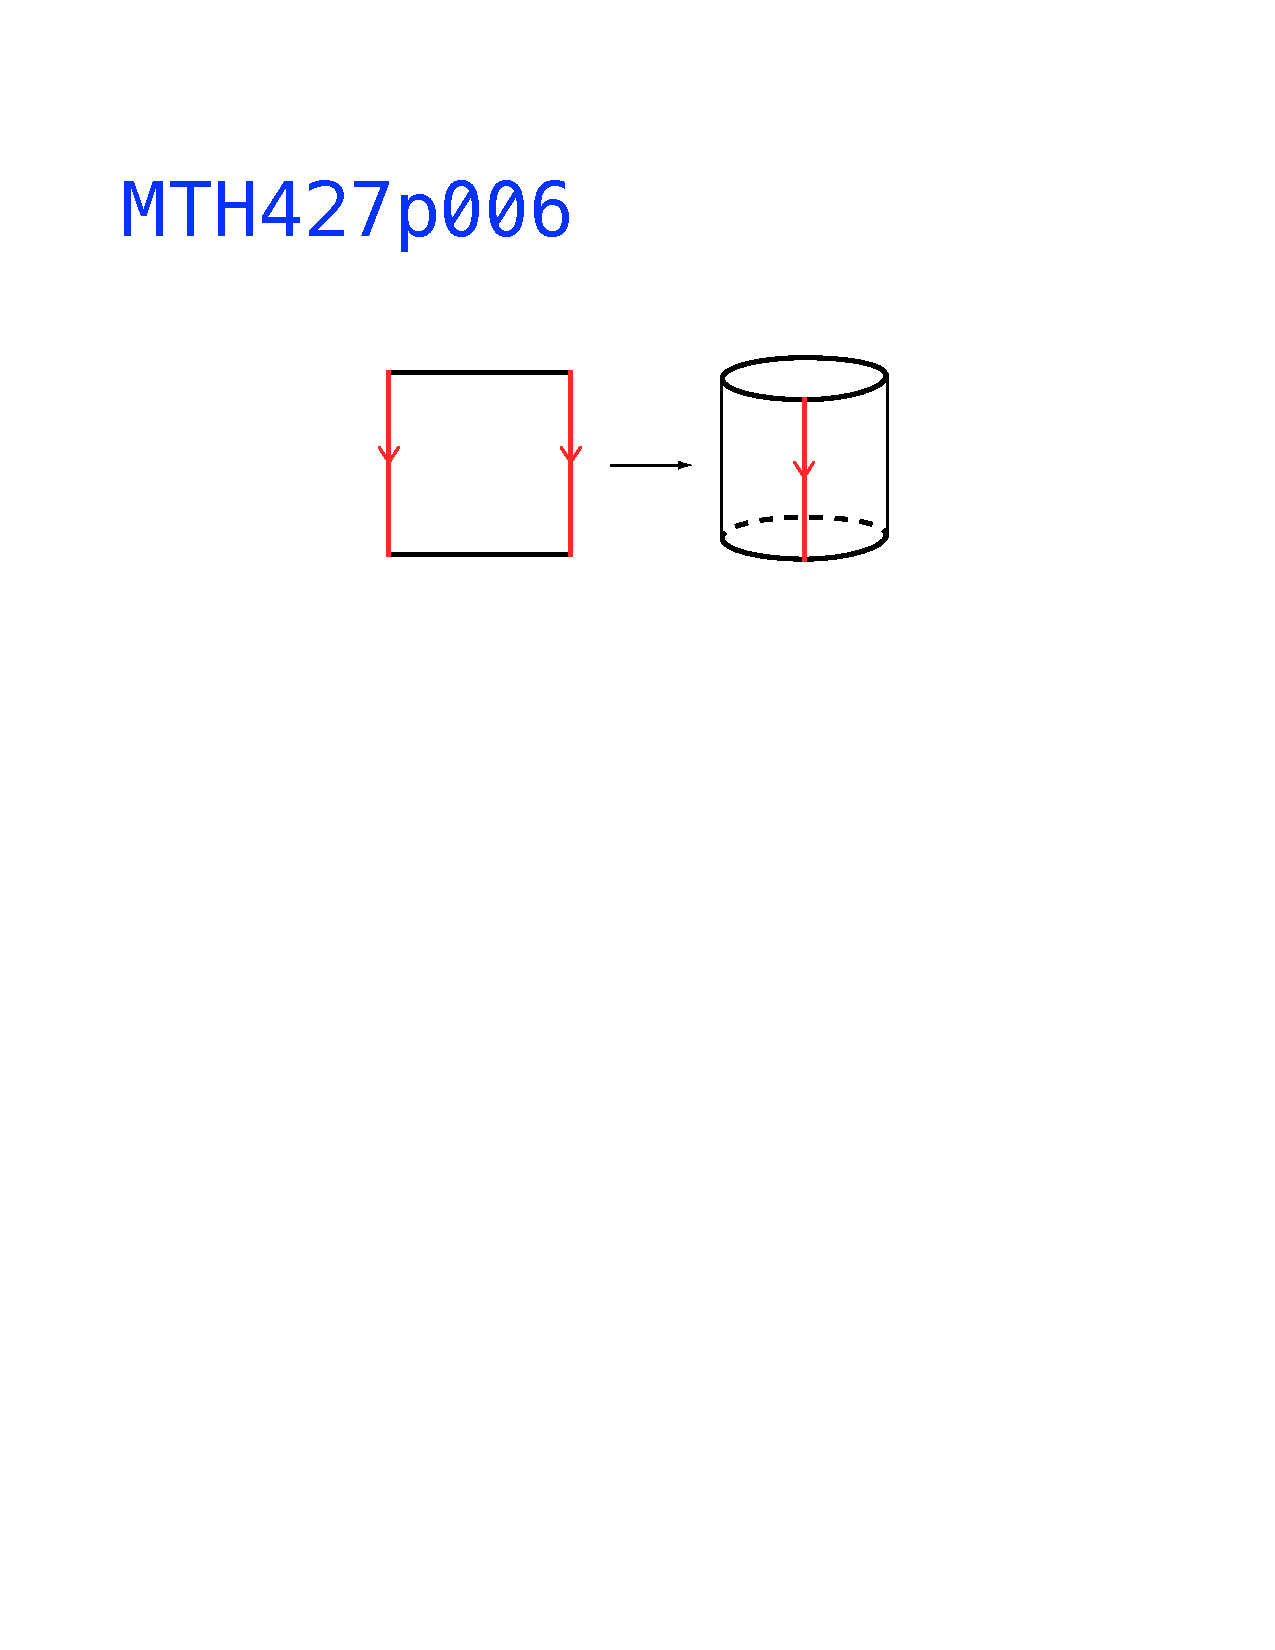
\includegraphics[width=\textwidth, trim=0mm 183mm 0mm 57mm, clip]{pictures/MTH427p006.pdf}}}

In order to make this precise we need to specify the following:
\benu
\item what are the points of $Y$; 
\item what is the topology on $Y$. 
\eenu

The first part is done by considering $Y$ as  the set of \emph{equivalence classes} of some 
\emph{equivalence relation} on $X$. The second part is done by defining the 
\emph{quotient topology}. We explain these notions below. 

%---BBLANK #
\begin{definition}
\index{relation! equivalence@{equivalence $\sim$}}
Let $X$ be a set. An \emph{equivalence relation on $X$} is a binary relation $\sim$ satisfying three 
properties:
\benu
\item $x\sim x$ for all $x\in X$ (reflexivity)
\item if $x\sim y$ then $y\sim x$ (symmetry)
\item  if $x\sim y$ and $y\sim z$ then $x\sim z$ (transitivity)
\eenu
\end{definition}
%---EBLANK #

\begin{example}
\label{EQUIV REL1 EXAMPLE}
Let $X = [0, 1]\times [0, 1]$. Define a relation on $X$ as follows. For any $(s,t)\in X$ we set 
$(s,t)\sim (s,t)$. Also, for any $t\in [0,1]$ we set $(0,t)\sim (1,t)$ and $(1,t)\sim (0,t)$. This relation is 
an equivalence relation that identifies corresponding points of the vertical edges of the square 
$[0, 1]\times [0,1]$.
\end{example}

\begin{example}
\label{EQUIV REL2 EXAMPLE}
Define a relation $\sim$ on the set of real numbers $\R$ as follows: $r\sim s$  if $s = r+n$
for some $n\in \Z$. One can check that this is an equivalence relation (exercise). 
\end{example}

%---BBLANK # \newpage
\begin{definition}
Let $X$ we a set with an equivalence relation $\sim$ and let $x\in X$. The \emph{equivalence class}
of $x$ is the subset $[x]\subseteq X$ consisting of all elements that are in the relation with $x$:
$$[x] = \{ y\in X \ | \ x\sim y\}$$ 
\end{definition}
%---EBLANK #

\begin{example}
Take $X= [0,1]\times [0,1]$ with the equivalence relation defined as in Example \ref{EQUIV REL1 EXAMPLE}. 
If $(s, t)\in X$ and $s\neq 0,1$ then $[(s,t)]$ consists of a single point: $[(s,t)] = \{(s,t)\}$. 
If $s = 0,1$ then $[(s,0)]$ consists of two points: $[(0,t)] = [(1,t)] = \{(0,t), (1,t)\}$.  
\end{example}

\begin{example}
Take $\R$ with the equivalence relation defined as in Example \ref{EQUIV REL2 EXAMPLE}. 
For $r\in \R$ we have:
$$[r] = \{r+n \ | \ n\in \Z\}$$
For example: $[1] = \{ 1+n \ | \ n\in \Z \} = \Z$. Notice that $[1] = [2] $ and 
$[\sqrt{2}] = [\sqrt{2}+1]$. 
\end{example}

%---BBLANK # \vskip 40mm
\begin{proposition}
\label{EQUIV CLASSES PROP}
Let $X$ be a set with an equivalence relation $\sim$, and let  $x, y\in X$. 
\benu
\item[1)] If $x\sim y$ then  $[x]=[y]$.
\item[2)] If $x\not\sim y$ then $[x]\cap [y]  = \varnothing$.
 \eenu
\end{proposition}
%---EBLANK #

\begin{proof}
1) Assume that $x\sim y$ and that $z\in [x]$. This gives $z\sim x$ and by transitivity $z\sim y$. 
Therefore $z\in [y]$. This shows that $[x]\subseteq [y]$. In the same way we can show that $[y]\subseteq [x]$. 
Therefore we get $[x]=[y]$.

2) Assume that  $[x]\cap [y]  \neq \varnothing$, and let $z \in [x]\cap [y]$. 
Then $x\sim z$ and $y\sim z$,  so by transitivity $x\sim y$ which contradicts our assumption. 
\end{proof}


\begin{note}
Proposition \ref{EQUIV CLASSES PROP} shows that an equivalence 
relation $\sim$ on a set $X$ splits $X$ into a disjoint union of distinct equivalence classes of $\sim$. 
The opposite is also true. Namely, assume that we have a family $\{A_{i}\}_{i\in I}$ of subsets of $X$ 
such that $A_{i}\cap A_{j} = \varnothing$ for $i\neq j$ and  $\bigcup_{i\in I}A_{i} = X$.  We can define 
a relation $\sim$ on $X$ such that $x\sim y$ if and only if both $x$ and $y$ are elements of the same subset $A_{i}$. 
This relation is an equivalence relation and its equivalence classes are the sets $A_{i}$. 
\end{note}

%---BBLANK # \vskip 30mm
\begin{definition}
Let $X$ be a set with an equivalence relation $\sim$. The \emph{quotient set} of $X$ is the set 
$X/{\sim}$ whose elements are all distinct equivalence classes of $\sim$. The function 
$$\pi \colon X \to X/{\sim}$$
given by $\pi(x) = [x]$ is called the \emph{quotient map}. 
\end{definition}
%---EBLANK #

\begin{note}
\label{QUOTIENT FUNCTION NOTE}
Let $X$ be a set with an equivalence relation $\sim$, and let $f\colon X \to Y$ be a function. 
Assume that for each $x, x'\in X$ such that $x\sim x'$ we have $f(x) = f(x')$. Then we can define 
a function $\overline{f}\colon X/{\sim} \to Y$ by $\overline{f}([x]) = f(x)$. We have $f = \overline f \pi$, 
i.e. the following diagram commutes:
\begin{equation*}
\begin{tikzpicture}
\matrix (m) 
[matrix of math nodes, row sep=3em, column sep=3em, text height=1.5ex, text depth=0.25ex]
{
& X/{\sim} \\
X & Y \\ 
};
\path[->, thick, font=\scriptsize]
(m-2-1) 
edge node[auto] {$\pi$} (m-1-2)
edge node[below] {$f$} (m-2-2)
(m-1-2)
edge node[auto] {$\overline{f}$} (m-2-2)
; 
\end{tikzpicture}
\end{equation*}
\end{note}

%---BBLANK # \newpage
\begin{definition}
Let $X$ be a topological space and let $\sim$ be an equivalence relation on  $X$. 
The \emph{quotient topology} on the set $X/{\sim}$ is the topology where a set $U\subseteq X/{\sim}$ 
is open  if and only if the set $\pi^{-1}(U)$ is open in $X$. The set $X/{\sim}$ with this topology is called the
 \emph{quotient space} of $X$ taken with respect to the relation $\sim$. 
\end{definition}
%---EBLANK #

%---BBLANK # \vskip 40mm
\begin{proposition}
\label{CLOSED SET QUOTIENT TOP PROP}
Let $X$ be a topological space and let $\sim$ be an equivalence relation on  $X$. A set $A\subseteq X/{\sim}$
is closed if and only  the set $\pi^{-1}(A)$ is closed in $X$. 
\end{proposition}

\begin{proof}
Exercise.
\end{proof}
%---EBLANK #

%---BBLANK # \vskip 20mm
\begin{proposition}
\label{QUOTIENT SPACE FUNCTIONS PROP}
Let $X, Y$ be a topological spaces  and let $\sim$ be an equivalence 
relation on $X$. A function $f\colon X/{\sim}\to Y$ is continuous if and only if the function $f\pi\colon X \to Y$ is 
continuous. 
\end{proposition}

\begin{proof}
Exercise. 
\end{proof}
%---EBLANK #

\begin{note}
\label{QUOTIENT SPACE FACTORIZATION NOTE}
Let $X$ be a space with an equivalence relation $\sim$ and let $f\colon X \to Y$ be a continuous function. 
If for each $x, x'\in X$ such that $x\sim x'$ we have $f(x) = f(x')$ then as in 
(\ref{QUOTIENT FUNCTION NOTE}) we obtain a function $\overline{f}\colon X/{\sim} \to Y$, 
$\overline{f}([x]) = f(x)$. Since the function $\overline{f}\pi = f$ is continuous thus by 
Proposition \ref{QUOTIENT SPACE FUNCTIONS PROP} $\overline{f}$ is a continuous function. 
\end{note}



\begin{example}
\label{INTERVAL MOD BOUNDARY EXAMPLE}
Take the closed interval $[-1,1]$ with the equivalence relation $\sim$ such that $(-1) \sim 1$
(and $t\sim t$ for all $t\in [-1,1]$). We will show that the quotient space $[-1.1]/{\sim}$ is homeomorphic to the 
circle $S^{1}$.   Consider the function $f\colon [-1,1]\to S^{1}$ given by 
$f(x) = (\sin \pi x, \ -\cos \pi x)$:

%\begin{tikzpicture}
%
%\node[anchor=south west,inner sep=0] at (0,0) 
%{\includegraphics[width=\textwidth, trim=0mm 171mm 0mm 57mm, clip]{pictures/Lec19p01.pdf}};
%
%%%% COORDINATE GRID
%%\draw[step=0.5, help lines] (0,0) to[grid with coordinates] (15,9);
%%%% 
%
%\node at (8.5,2.2){\small $f$};
%\node at (4.8,1.5){\small $0$};
%\node at (5.8,1.5){\small $\tfrac{1}{2}$};
%\node at (6.82,1.5){\small $1$};
%\node at (3.65,1.5){\small $-\tfrac{1}{2}$};
%\node at (2.62,1.5){\small $-1$};
%\node at (12.35,0.15){\small $f(0)$};
%\node at (13.85,1.6){\small $f(\tfrac{1}{2})$};
%\node at (9.98, 1.6){\small $f(-\tfrac{1}{2})$};
%\node at (13.01, 3.65){\small $f(-1) = f(1)$};
%\end{tikzpicture}

 
Since $f(1) = f(-1)$  by (\ref{QUOTIENT SPACE FACTORIZATION NOTE}) we get the induced 
continuous function $\overline{f}\colon [-1,1]/{\sim} \to S^{1}$. We will prove that $\overline{f}$ is a homeomorphism. First, notice that $\overline{f}$ is a bijection.  Next, since $[-1, 1]$  
is a compact space and the quotient map $\pi\colon [-1,1] \to [-1, 1]/{\sim}$ is onto  by 
Proposition \ref{COMPACT ONTO PROP} we obtain that the space $[-1,1]/{\sim}$ is compact.  
Therefore we can use Proposition \ref{COMPACT TO HAUSDORF BIJ PROP} which says 
that any continuous bijection from a compact space to a Hausdorff space  is a homeomorphism. 

This example can be generalized as follows. Take the closed unit ball 
$$\xov{B}^{n} = \{ x\in \R^{n} \ | \ d(0, x) \leq 1 \}$$
The unit sphere $S^{n-1} = \{ x\in \R^{n} \ | \ d(0, x) = 1 \}$ is a subspace of $\xov{B}^{n}$. 
Consider the equivalence relation $\sim$ on $\xov{B}^{n}$ that identifies all points of $S^{n-1}$: 
$x\sim x'$ for all $x, x' \in S^{n-1}$. 
Using  similar arguments as above one can show that $\xov{B}^{n}/{\sim}$ is homeomorphic to the 
sphere $S^{n}$  (exercise). Notice that for $n=1$ we have $\xov{B}^{1} = [-1, 1]$ and $S^{0} = \{-1, 1\}$ 
so in this case we recover the homeomorphism $[-1, 1]/{\sim}\cong S^{1}$. 

\end{example}

\begin{note}
Let $X$ be a space and let $A\subseteq X$. Consider the equivalence relation on $X$ that identifies 
all points of $A$: $x\sim x'$ for all $x, x'\in A$. The quotient space $X/{\sim}$ is usually denoted by $X/A$. 
Using this notation the homeomorphism given in Example  \ref{INTERVAL MOD BOUNDARY EXAMPLE} 
can be written as $\xov{B}^{n}/S^{n-1}\cong S^{n}$. 
\end{note}




%---BBLANK # \newpage
\begin{example}
Take the square $[0,1]\times [0,1]$ with the equivalence relation defined as in 
Example \ref{EQUIV REL1 EXAMPLE}:  $(0,t)\sim (1,t)$ for all $t\in [0,1]$. Using arguments similar as 
in Example \ref{INTERVAL MOD BOUNDARY EXAMPLE} we can show that the quotient space is 
homeomorphic to the cylinder $S^{1}\times [0,1]$:

{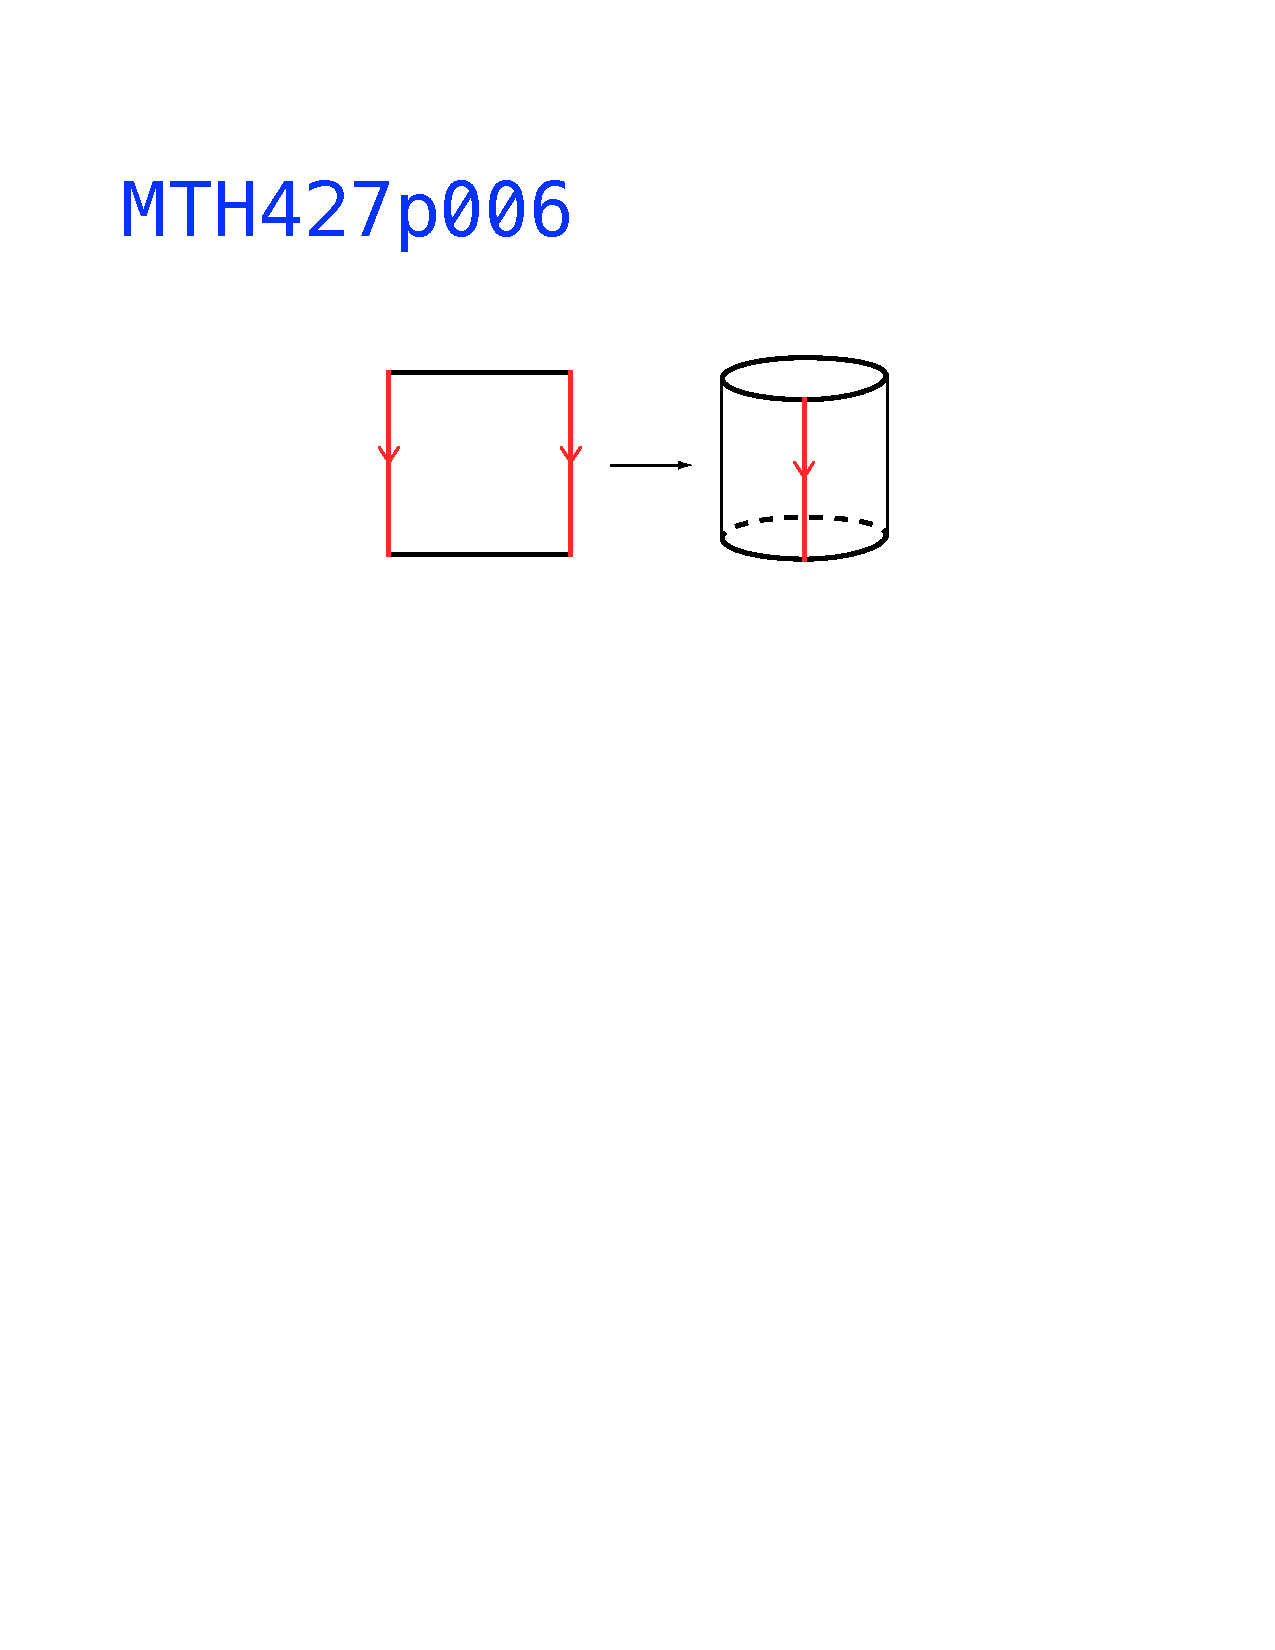
\includegraphics[width=\textwidth, trim=0mm 183mm 0mm 57mm, clip]{pictures/MTH427p006.pdf}}   
\end{example}
%---EBLANK # 

%---BBLANK # \vskip 40mm
\begin{example}
Take the square $[0,1]\times [0,1]$ with the equivalence relation given by $(0,t)\sim (1, 1-t)$
for all $t\in [0,1]$. The space obtained as a quotient space is called the \emph{M\"obius band}:

{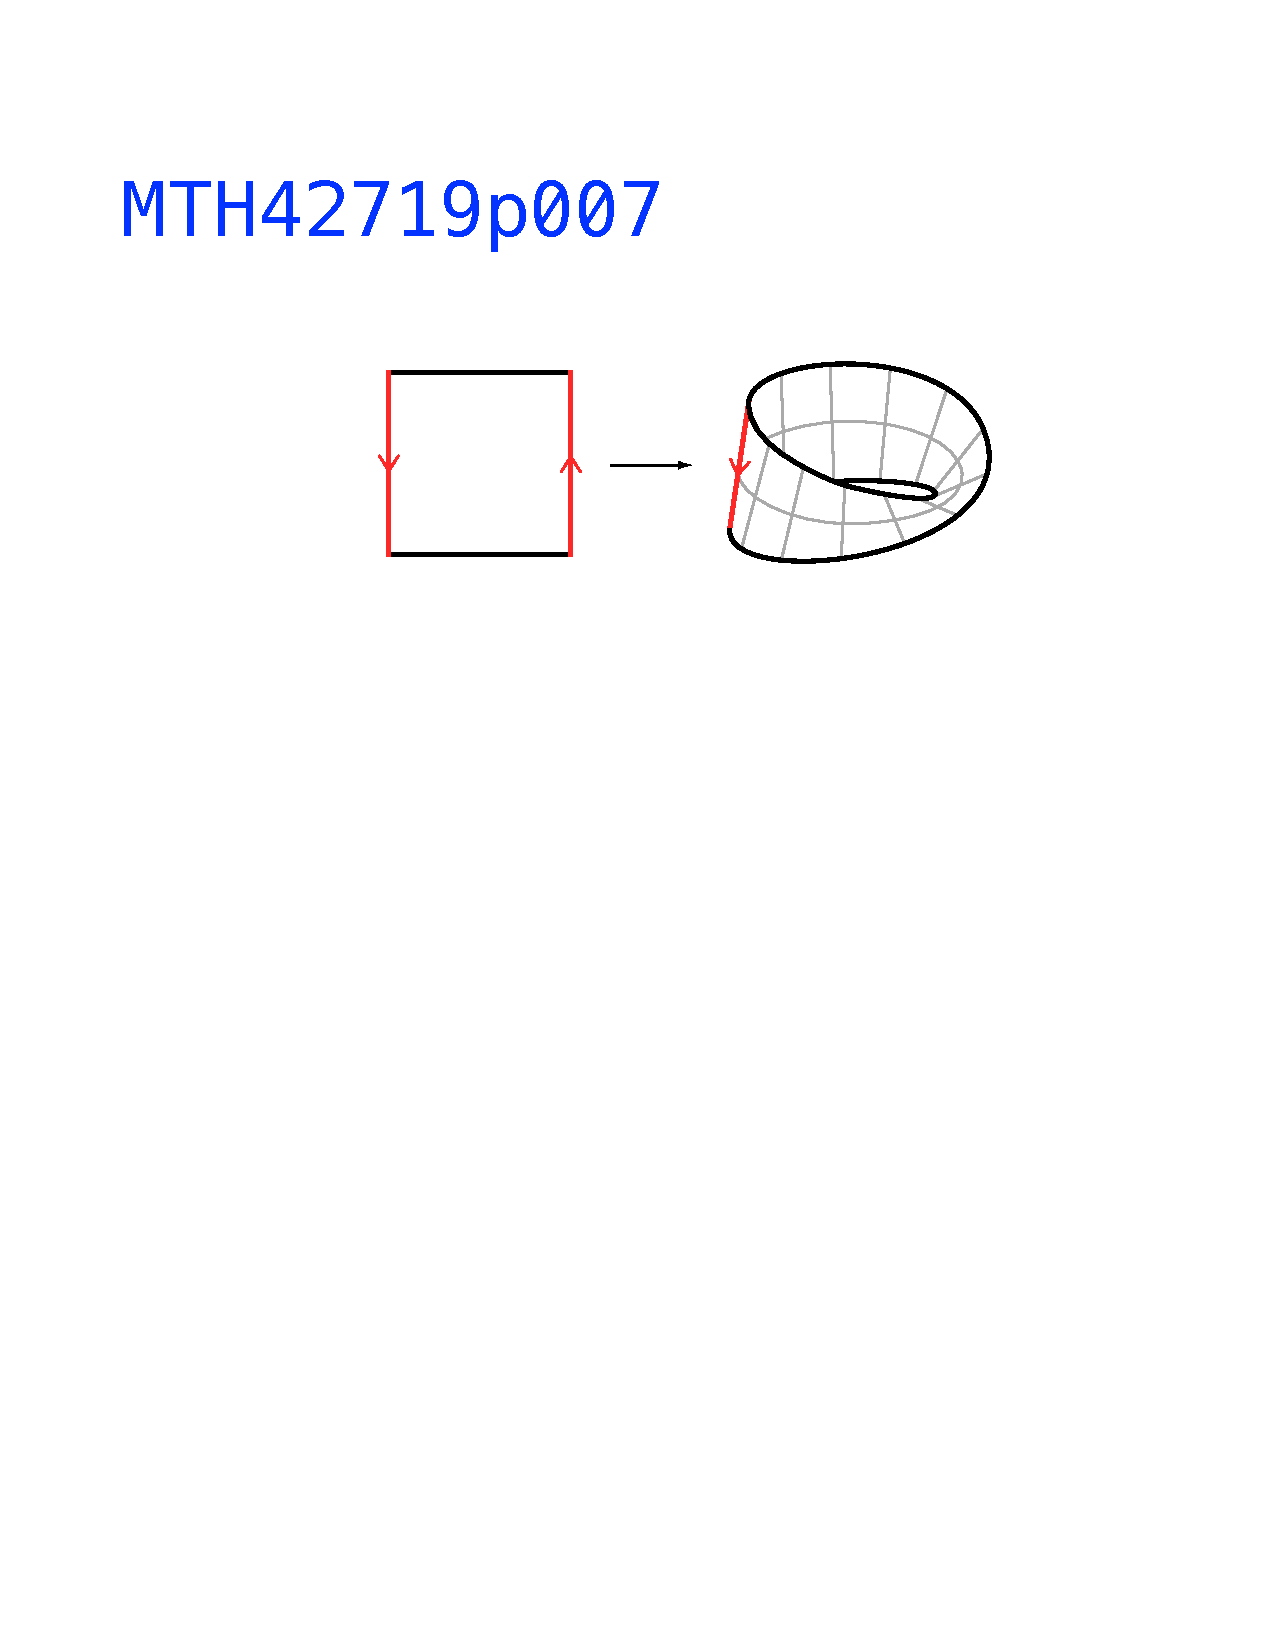
\includegraphics[width=\textwidth, trim=0mm 183mm 0mm 60mm, clip]{pictures/MTH427p007.pdf}}   
%---EBLANK # \end{example}

The M\"obius band is a $2$-dimensional manifold with boundary, and its boundary is homeomorphic
to $S^{1}$. 
\end{example}

%---BBLANK # \newpage
\begin{example}
Take the square $[0,1]\times [0,1]$ with the equivalence relation given by $(0,t)\sim (1, t)$
for all $t\in [0,1]$ and $(s, 0)\sim (s,1)$ for all $s\in [0,1]$. Using arguments similar to these given in 
Example \ref{INTERVAL MOD BOUNDARY EXAMPLE} one can show that the quotient space in this 
case is homeomorphic to the torus:

{{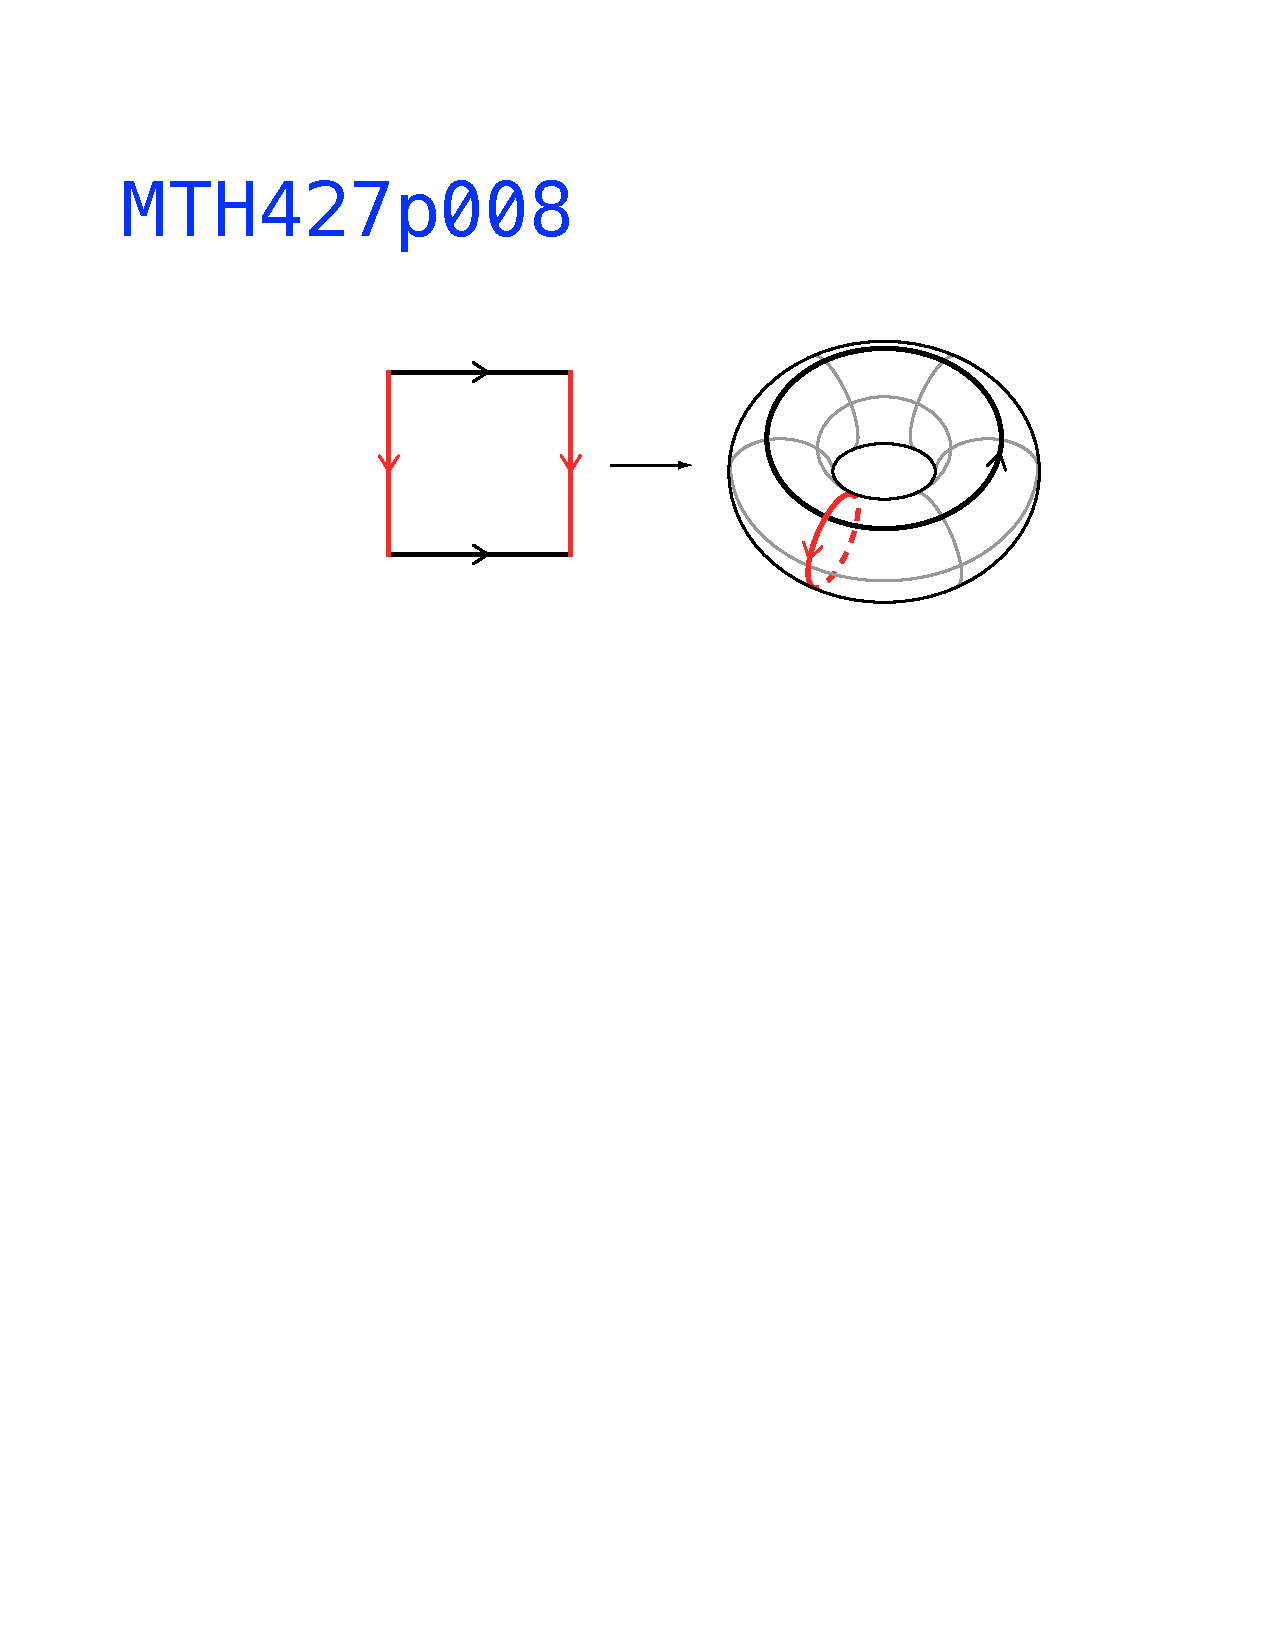
\includegraphics[width=\textwidth, trim=0mm 176mm 0mm 57mm, clip]{pictures/MTH427p008.pdf}}   }

\end{example}
%---EBLANK # 

%---BBLANK # \vskip 40mm
\begin{example}
\label{KLEIN BOTTLE EXAMPLE}
Take the square $[0,1]\times [0,1]$ with the equivalence relation given by $(0,t)\sim (1, t)$
for all $t\in [0,1]$ and $(s, 0)\sim (1-s,1)$ for all $s\in [0,1]$. The resulting quotient space 
is called the \emph{Klein bottle}. One can show that the Klein bottle is a two dimensional manifold. 

{{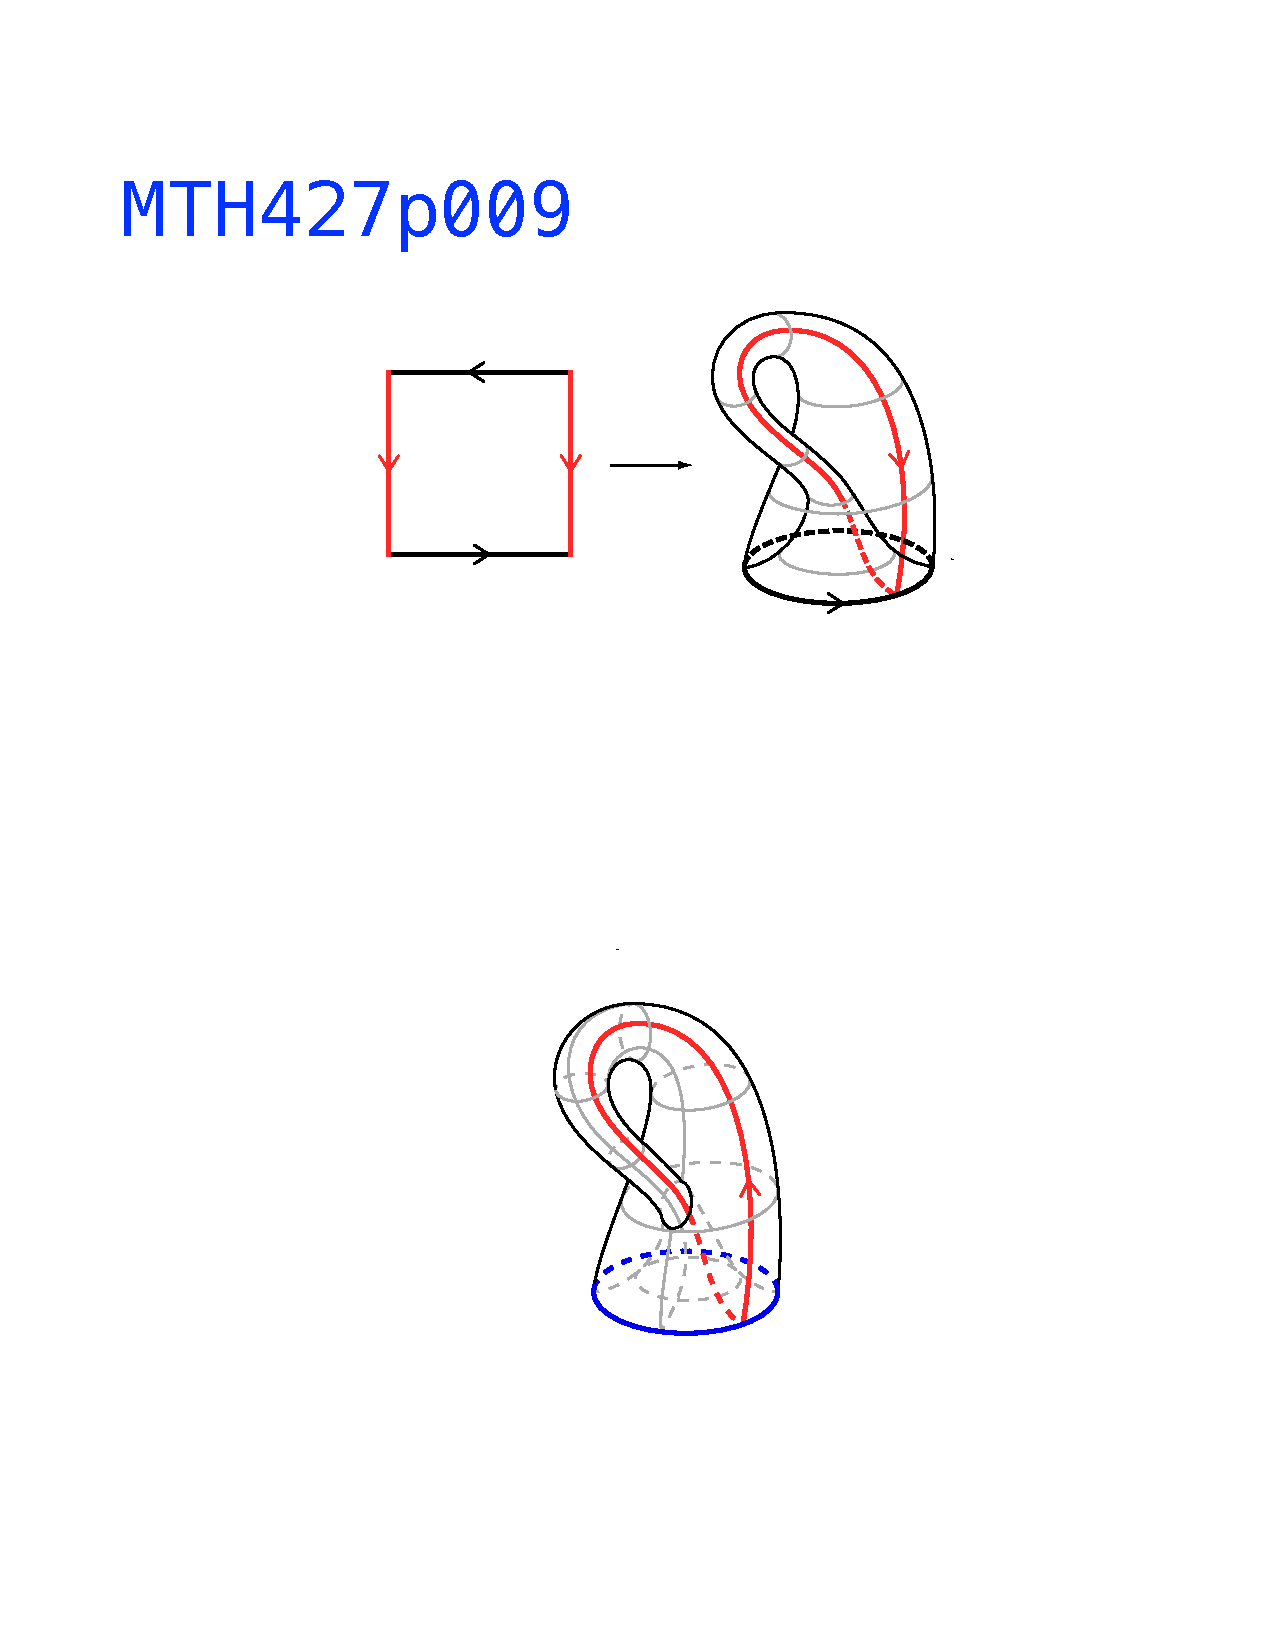
\includegraphics[width=\textwidth, trim=0mm 176mm 0mm 51mm, clip]{pictures/MTH427p009.pdf}}}   

\end{example}
%---EBLANK # 

%---BBLANK # \newpage
\begin{example}
\label{RP2 EXAMPLE}
Following the scheme of the last two examples we can consider the square
$[0,1]\times [0,1]$ with the equivalence relation given by $(0,t)\sim (1, 1-t)$
 and $(s, 0)\sim (1-s,1)$ for all $s, t\in [0,1]$:

{{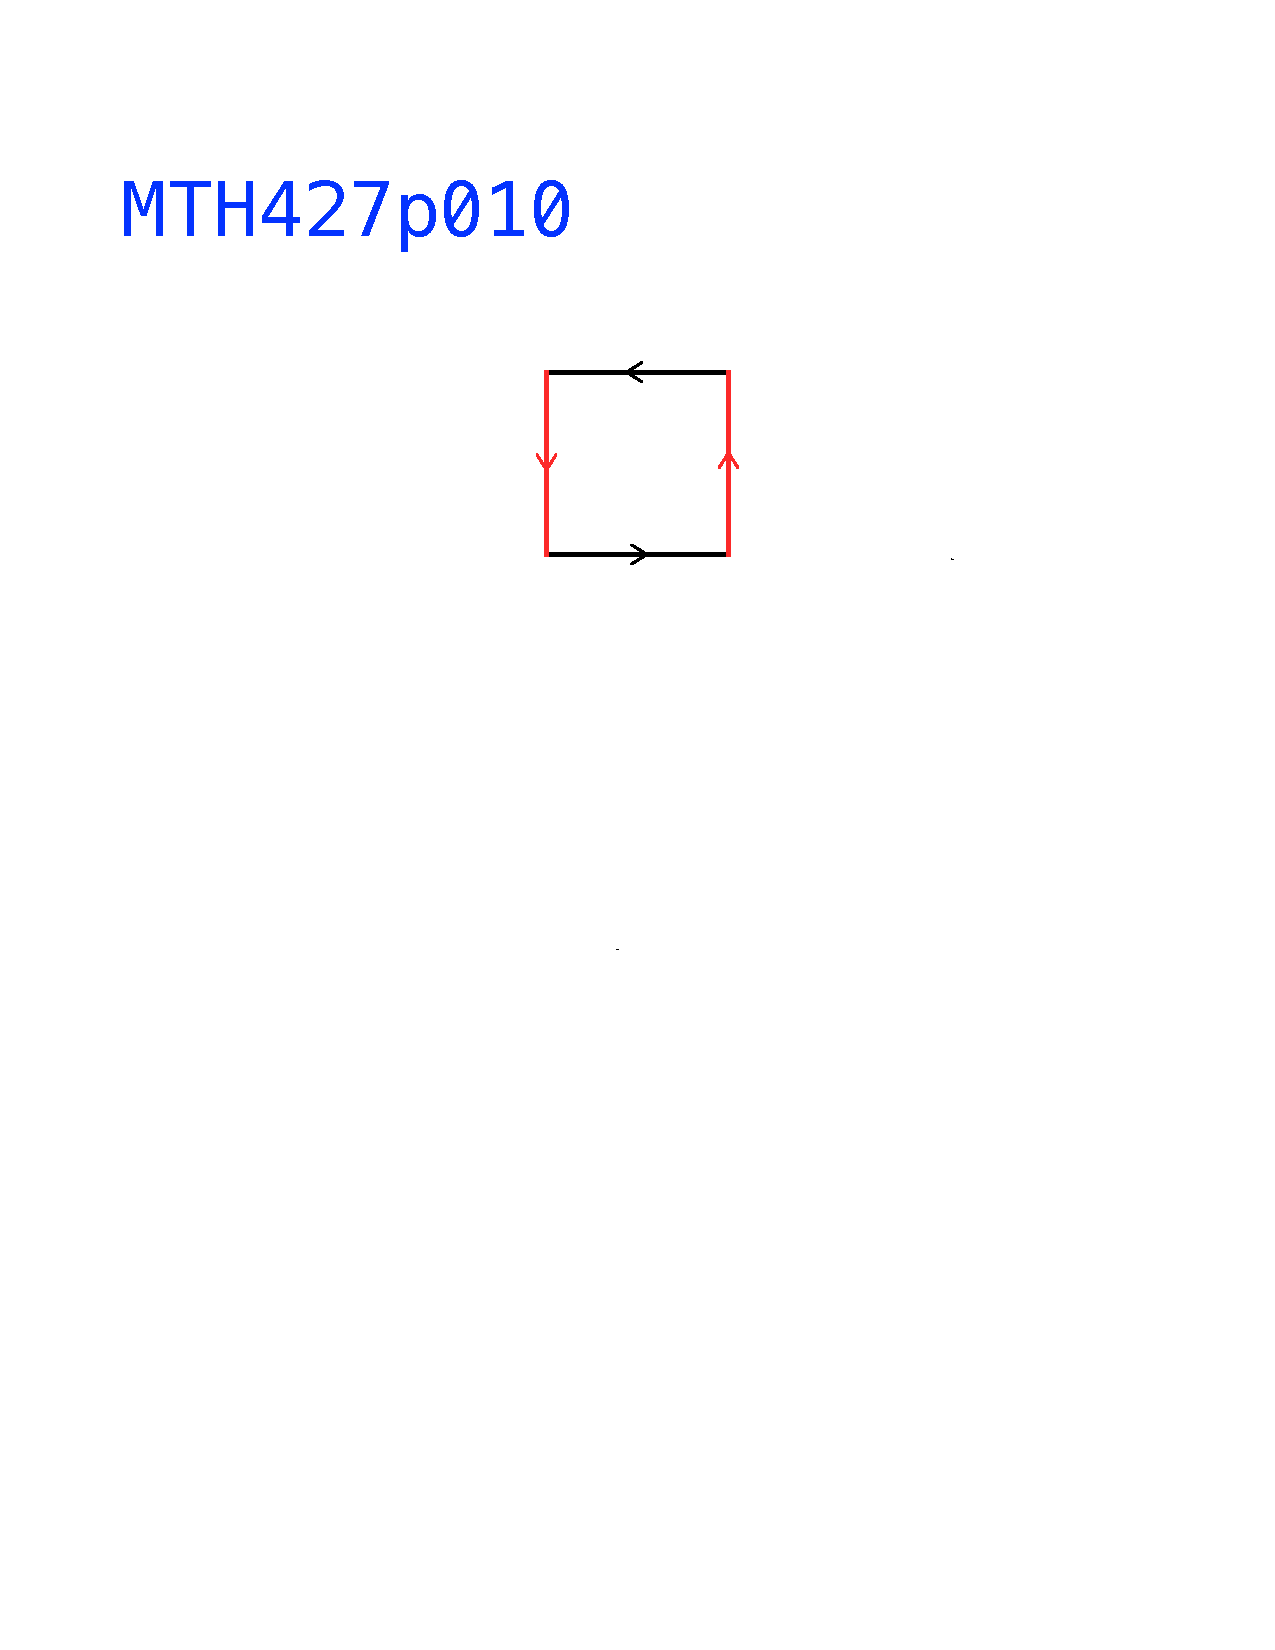
\includegraphics[width=\textwidth, trim=0mm 183mm 0mm 60mm, clip]{pictures/MTH427p010.pdf}}}   
%---EBLANK # \end{example}

The resulting quotient space is homeomorphic to the space $\RP^{2}$
which is defined as follows. Take the the $2$-dimensional closed unit ball $\overline{B}^{2}$. 
The boundary of $\overline{B}^{2}$ is the circle $S^{1}$. Consider the equivalence relation $\sim$ 
on $\overline{B}^{2}$ that identifies each point $(x_{1}, x_{2})\in S^{1}$ with its antipodal point 
$(-x_{1}, -x_{2})$:

{{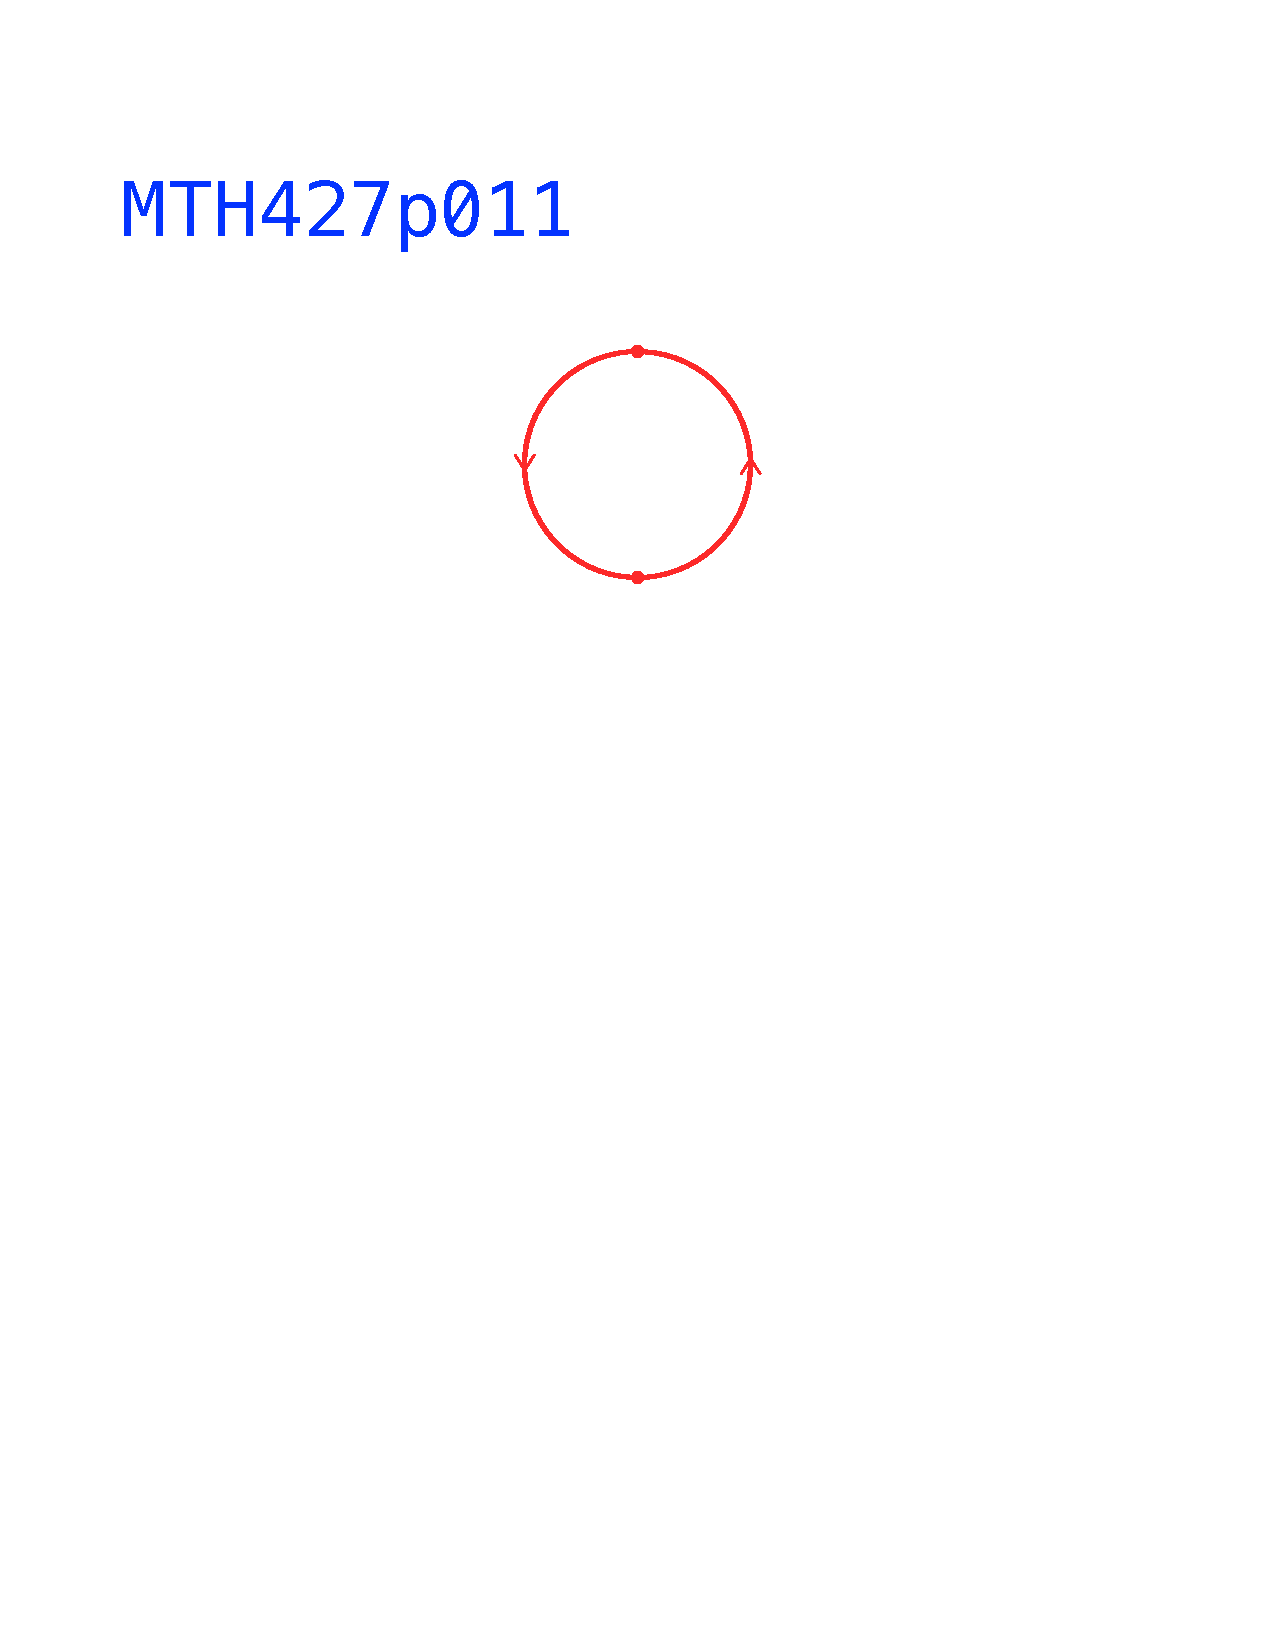
\includegraphics[width=\textwidth, trim=0mm 180mm 0mm 58mm, clip]{pictures/MTH427p011.pdf}}} 

We define $\RP^{2} = \overline{B}^{2}/{\sim}$. This space is called the \emph{2-dimensional real projective space} and  it is a 2-dimensional manifold. 
One can show that $\RP^{2}$  (and also the Klein bottle) cannot be embedded into $\R^{3}$. For 
this reason it is harder to visualize it.


\end{example}


\begin{example}
\label{RPN EXAMPLE}
The construction of $\RP^{2}$ given in Example \ref{RP2 EXAMPLE}  can be generalized to higher dimensions. 
Consider the $n$-dimensional closed unit ball $\overline{B}^{n}$. The boundary 
$\overline{B}^{n}$ is the sphere $S^{n-1}$. Similarly as before we can consider the equivalence 
relation $\sim$ on $\overline{B}^{n}$  that identifies antipodal points of $S^{n-1}$:
$$(x_{1}, \dots, x_{n})\sim (-x_{1}, \dots, -x_{n})$$
for all $(x_{1}, \dots, x_{n})\in S^{n-1}$. The quotient space $\overline{B}^{n}/{\sim}$ is denoted by 
$\RP^{n}$ and is called the \emph{n-dimensional real projective space}. The space $\RP^{n}$
is an $n$-dimensional manifold.  
For another perspective on projective spaces see Exercise \ref{RPN CONSTRUCTION EXERCISE}.  
\end{example}


Many  constructions in topology involve the following setup. We start with two
topological spaces $X_{1}$, $X_{2}$, and we build a new space $Y$ by identifying certain points of $X_{1}$
with certain points  of $X_{2}$:

%---BBLANK # \newpage {\bf Disjoint unions} \ \vskip 10mm
\begin{equation*}
\begin{tikzpicture}[scale = 1]
\draw[line width = 1.5pt] (0, 0) arc (90:270:1) node[ pos = 0.7, anchor = north east] {\small $X_{1}$};
\draw[line width = 1.5pt] (1.5, 0) arc (90:-90:1)  node[ pos = 0.7, anchor = north west] {\small $X_{2}$};
\draw[line width = 1.5pt] (6, -1) circle (1);
\node at (7, -1.86) {\small $Y$};
\fill[red] (0,0) circle (0.1);
\fill[red] (0,-2) circle (0.1);
\fill[red] (1.5,0) circle (0.1);
\fill[red] (1.5,-2) circle (0.1);
\fill[red] (6,0) circle (0.1);
\fill[red] (6,-2) circle (0.1);
\draw[red, <->, >=latex] (0.3, 0) -- (1.2, 0); 
\draw[red, <->, >=latex] (0.3, -2) -- (1.2, -2); 
\draw[thick, ->, >=latex] (3.2, -1) -- (4.3, -1); 
\end{tikzpicture}
\end{equation*}
%---EBLANK # 

An example of a setting that uses such assembly process is described 
in Chapter \ref{SIMPLICIAL COMPLEXES CH}.

The first step in constructions of this kind it to create a new space $X_{1}\sqcup X_{2}$
which contains $X_{1}$ and $X_{2}$ as its subspaces. The space $Y$  can be 
then described as a quotient space of $X_{1}\sqcup X_{2}$. The space $X_{1}\sqcup X_{2}$
is defined as follows. If $X_{1}\cap X_{2} = \varnothing$ then 
$X_{1}\sqcup X_{2} = X_{1}\cup X_{2}$ as a set. A set $U\subseteq X_{1}\sqcup X_{2}$ is open
if and only if $U\cap X_{i}$ is open in $X_{i}$ for $i = 1, 2$.  If $X_{1}\cap X_{2}\neq \varnothing$
then we first replace $X_{i}$ with a homeomorphic space $X_{i}'$ such that $X_{1}'\cap X_{2}' = \varnothing$
(e.g. we can take $X_{i}' = \{i\}\times X_{i}$) and then we set $X_{1}\sqcup X_{2}$ to be equal to $X'_{i}\sqcup X_{2}'$.  


\begin{definition}
The space $X_{1}\sqcup X_{2}$ is called the \emph{disjoint union} (or the \emph{coproduct})
of spaces $X_{1}$ and $X_{2}$. 
\end{definition}


\begin{example}
Take $X_{1} = (0, 1)$ and $X_{1} = [1, 2)$. Since $X_{1}\cap X_{2} = \varnothing$ we can construct the space
$(0, 1) \sqcup [1, 2)$ so that it consists of the points of the interval $(0, 2)$. However,  the disjoint union 
$(0, 1) \sqcup [1, 2)$ is not homeomorphic to the interval $(0, 2)$ taken with the usual topology. For example, the set 
$U = [1, \frac{1}{2})$ is not open in the interval $(0, 2)$, but it is open in $(0, 1) \sqcup [1, 2)$ since 
$U\cap (0, 1) = \varnothing$ is open in  $(0, 1)$ and 
$U\cap [1, 2) = [1, \frac{1}{2})$ is open in  $[1, 2)$.  In general,  in the disjoint union $X_{1}\sqcup X_{2}$ the 
spaces $X_{1}$ and $X_{2}$ can be imagined as being far apart from each other so that an arbitrary combination 
of an open set in $X_{1}$ and and open set in $X_{1}$ gives an open set in $X_{1}\sqcup X_{2}$. For example, 
the space $(0, 1) \sqcup [1, 2)$ is homeomorphic to the subspace of $\R^{2}$ given by 
$(0, 1) \times \{-a\} \cup [1, 2)\times \{a\}$ for some $a>0$.  

\begin{equation*}
\begin{tikzpicture}[scale = 2] 
\draw[->, >=latex, thick] (-0.4,0) -- (2.5,0);
\draw[->, >=latex, thick] (0, -0.5) -- (0 , 0.5);
\draw[line width = 3pt, red] (0, -0.3) -- (1,-0.3);
\draw[line width = 3pt, red] (1, 0.3) -- (2,0.3);
\draw[line width = 1.5pt, red, fill=white] (0,-0.3) circle (0.05);
\draw[line width = 1.5pt, red, fill=white] (1,-0.3) circle (0.05);
\draw[line width = 1.5pt, red, fill=red] (1,0.3) circle (0.05);
\draw[line width = 1.5pt, red, fill=white] (2,0.3) circle (0.05);

\end{tikzpicture}
\end{equation*}

\end{example}


The construction of a disjoint union can be extended to  arbitrary families of topological spaces. 
Given a family $\{X_{i}\}_{i\in I}$ such that $X_{i}\cap X_{j}  = \varnothing$ for all $i\neq j$, we 
define $\bigsqcup_{i\in I} X_{i} = \bigcup_{i\in I} X_{i}$ as a set. A set $U \subseteq \bigsqcup_{i\in I} X_{i}$ is 
open if and only if the set $U\cap X_{i}$ is open in $X_{i}$ 
for each $i\in I$. If the family  $\{X\}_{i\in I}$ does not consist of disjoint spaces, then 
we first replace it with a family $\{X_{i}'\}_{i\in I}$ such that $X_{i}'\cong X_{i}$ for each $i\in I$, and $X_{i}'\cap X_{j}'  = \varnothing$ for all $i\neq j$. 

If $\bigsqcup_{i\in I} X_{i}$ is the disjoint union of a family $\{X_{i}\}_{i\in I}$,  then for each
$j\in I$ we have an embedding $k_{j}\colon X_{j} \to \bigsqcup_{i\in I} X_{i}$. The following fact is
an essential property of the space $\bigsqcup_{i\in I} X_{i}$:


\begin{proposition}
\label{COPROD OF FUNCTIONS PROP}
For any family of continuous functions  $\{f_{i}\colon X_{i}  \to Y\}_{i\in I}$, there exists a unique continuous 
function $f\colon \bigsqcup_{i\in I} X_{i} \to Y$ such that $k_{j}f = f_{j}$ for each $j\in I$.
\end{proposition}


\begin{proof}
Exercise. 
\end{proof}


\begin{note}
The function $f\colon \bigsqcup_{i\in I} X_{i} \to Y$ in Proposition \ref{COPROD OF FUNCTIONS PROP}  
is usually denoted by $ \bigsqcup_{i\in I} f_{i}$. 

\end{note}



%%%%%%%%%%%%%%%%%%%%%%%%%%%%%%%
%  EXERCISES
%%%%%%%%%%%%%%%%%%%%%%%%%%%%%%%

\exercises

\begin{exercise}
Prove Proposition \ref{CLOSED SET QUOTIENT TOP PROP}.
\end{exercise}


\begin{exercise}
Prove Proposition \ref{QUOTIENT SPACE FUNCTIONS PROP}.
\end{exercise}





\begin{exercise}
Consider the real line $\R$ with the equivalence relation defined  as in Example \ref{EQUIV REL2 EXAMPLE}. 
Show that the quotient space $\R/{\sim}$ is homeomorphic with $S^{1}$. 
\end{exercise}


\begin{exercise}
Take the closed interval $[0,1]$ with the equivalence relation $\sim$ defined as in 
Example \ref{INTERVAL MOD BOUNDARY EXAMPLE}. Let 
$\pi\colon [0,1] \to [0,1]/{\sim}$ be the quotient map. The set $U=[0, \frac{1}{2})$
which is open subset  of $[0,1]$. Show that $\pi(U)$ is not open in $[0,1]/{\sim}$.
\end{exercise}




\begin{exercise}
Let $\xov{B}^{n} \subseteq \R^{n}$ be the closed unit ball 
(see Example \ref{INTERVAL MOD BOUNDARY EXAMPLE}). Show that $\xov{B}^{n}/S^{n-1}$ is homeomorphic
to $S^{n}$.  
\end{exercise}





\begin{exercise}
Let $X$ be a compact Hausdorff space, and let $U\subseteq X$ be an open set. Show that the 
one-point compactification $U^{+}$ of $U$ (\ref{ONEPOINTCOMPACTIF DEF}) is homeomorphic 
to the quotient space $X/(X\ssmin U)$.
\end{exercise}






\begin{exercise}
Recall that the topologists sine curve $Y$ is the subspace of $\R^{2}$ consisting of the vertical line segment
$Y_{1} = \{(0, y) \ | \ -1\leq y \leq 1\}$  and the curve $Y_{2} = \{(x, \sin(\tfrac{1}{x}))  \ | \ x>0  \}$:
\begin{equation*}
\begin{tikzpicture}[scale =1] 
\draw[line width = 1.5] (2.1, -1.03) -- (2.1, 1.03);
\begin{scope}
\draw[xscale=15, line width = 1.5 , domain= 0.151:0.4,smooth,variable=\x, samples = 400] plot ({\x},{sin(pow(\x, -2) r)});
\end{scope}
\node at (1.8, 0.88){\small $ Y_{1}$};
\node at (5.9, 0.88){\small $ Y_{2}$};
\end{tikzpicture}
\end{equation*}
Show that the space $Y/Y_{1}$ is homeomorphic to the  half line $[0, +\infty)$.
\end{exercise}








\begin{exercise}
\label{RPN CONSTRUCTION EXERCISE}
Consider the unit sphere $S^{n}$ with the equivalence relation that identifies 
antipodal points of $S^{n}$: 
$$(x_{1}, \dots, x_{n+1})\sim (-x_{1}, \dots, -x_{n+1})$$
for all $(x_{1}, \dots, x_{n+1})$. Show that the quotient space $S^{n}/{\sim}$ is homeomorphic to 
the projective space $\RP^{n}$ (\ref{RPN EXAMPLE}).

Note: This construction lets us interpret $\RP^{n}$ as the space of straight lines in $\R^{n+1}$ that 
pass through the origin. Indeed, any such line $L$ intersects the sphere $S^{n}$ at two points:
some point $x$ and its antipodal point $-x$: 

\begin{equation*}
\begin{tikzpicture}[scale = 1] 
\draw[opacity = 0] (-5, 0) -- (5, 0);
\draw[->,  >=latex, mygray4, thick] (-2, 0) -- (2,0);
\draw[->,  >=latex, mygray4, thick] (0, -2) -- (0, 2);
\draw[name path = main circle, line width = 1.5] (0, 0) circle (1.5);
\draw [name path = skew line] (-1.7, -1.7) -- (1.7, 1.7);
\path [name intersections = {of = main circle and skew line, name = i}];
\fill[color = red] (i-1) circle (0.1) node[right, xshift = 1] {\small $x$}; 
\fill[color = red] (i-2) circle (0.1) node[left, xshift = -1] {\small $-x$}; 
\node at (1.3, 1.6) {\small $L$}; 
\end{tikzpicture}
\end{equation*}

Since $\RP^{n}$ is obtained by identifying antipodal points we get a bijective correspondence 
between elements of $\RP^{n}$ and lines in $\R^{n+1}$ passing through the origin.  
\end{exercise}





\begin{exercise}
A \emph{pointed topological space} is a pair $(X, x_{0})$ where $X$ is a topological space and 
$x_{0} \in X$. 
The \emph{smash product} of pointed spaces $(X, x_{0})$ and $(Y, y_{0})$ is the 
quotient space 
$$X \wedge Y = (X\times Y)/A$$
where $A = (X\times \{y_{0}\}) \cup (\{x_{0}\} \times Y)$

a) Let $X, Y$ be a locally compact spaces (\ref{LOCALLY COMPACT DEF}). 
Show that the space $X\times Y$ is locally compact. 

b) By part a) and Corollary \ref{PROD HAUS COMP COR} if $X, Y$ are locally compact 
Hausdorff spaces then the space $X\times Y$ is also locally compact and Hausdorff. 
By Theorem \ref{ONE POINT COMPACT THM}  we have in such case one-point compactifications 
$X^{+}$, $Y^{+}$, and $(X\times Y)^{+}$ of the spaces $X$, $Y$, and $X\times Y$ respectively. 
Recall that $X^{+} = X \cup \{\infty\}$ and $Y^{+} = Y\cup \{\infty\}$. Consider 
$(X^{+}, \infty)$ and $(Y^{+}, \infty)$ as pointed spaces. Show that there is a homeomorphism:
$$X^{+}\wedge Y^{+} \cong (X\times Y)^{+}$$ 
\end{exercise}


\begin{exercise}
Prove Proposition \ref{COPROD OF FUNCTIONS PROP}. 
\end{exercise}


\begin{exercise}
Let $\{X_{i}\}_{i\in I}$ be a family of topological spaces, let $Z$ be a topological space 
and  for each $i\in I$ let $g_{i}\colon X_{i} \to Z$ let be a continuous function. Assume 
that for each family of continuous function functions $\{f_{i}\colon X_{i} \to Z\}_{i\in I}$ 
there exists a unique function $f\colon Z \to Y$ such that $g_{i}f  = f_{i}$ for each $i\in I$. 
Show that the space $Z$ is homeomorphic to  $\bigsqcup_{i\in I} X_{i}$. 
\end{exercise}


\begin{exercise}
The \emph{Hawaiian earring} space is a subspace $X \subseteq \R^{2}$ given by 
$X  = \bigcup_{n=1}^{\infty} C_{n}$ where $C_{n}$ is the circle with radius $\frac{1}{n}$
and center at the point $(0, \frac{1}{n})$:

\begin{equation*}
\begin{tikzpicture}
\draw[->,  >=latex, mygray4, thick] (-0.5, 0) -- (4.5,0);
\draw[->,  >=latex, mygray4, thick] (0, -2) -- (0, 2);
\draw[very thick] (2, 0) circle (2);
\draw[very thick] (2/2, 0) circle (2/2);
\draw[very thick] (2/3, 0) circle (2/3);
\draw[very thick] (2/4, 0) circle (2/4);
\draw[very thick] (2/5.5, 0) circle (2/5.5);
\draw[very thick] (2/8.5, 0) circle (2/8.5);
\draw[very thick] (2/15, 0) circle (2/15);
\fill (0, 0) circle (0.1) node[anchor= north east] {\small $(0, 0)$};
\end{tikzpicture}
\end{equation*}
Notice that the point $(0, 0)$ is the intersection of all circles $C_{n}$. 

For $n=1, 2, \dots$ let $C_{n}$ be the circle defined as above, and let $Y$ be the quotient space  of 
the disjoint union $\bigsqcup_{i=1}^{\infty} C_{n}$ obtained by identifying points  $(0, 0)\in C_{n}$ 
for all $n$. Show that $Y$ is not homeomorphic to $X$. 
\end{exercise}











\begin{exercise}
Let $\R^{n}_{+}$, $\R^{n}_{-}$, $\R^{n}_{0}$ be subspaces of $\R^{n}$ given by 
\begin{align*}
\R^{n}_{+} = \{(x_{1}, \dots, x_{n})\in \R^{n} \ | \ x_{n} \geq 0\}\\
\R^{n}_{-} = \{(x_{1}, \dots, x_{n})\in \R^{n} \ | \ x_{n} \leq 0\}\\
\R^{n}_{0} = \{(x_{1}, \dots, x_{n})\in \R^{n} \ | \ x_{n} = 0\}
\end{align*}
Notice that $\R^{n}_{0}$ is contained  in both $\R^{n}_{+}$ and $\R^{n}_{-}$. Given a homeomorphism   
$h\colon \R^{n}_{0} \to \R^{n}_{0}$ let $\R^{n}_{+}\cup_{h} \R^{n}_{-}$ denote the quotient space
$(\R^{n}_{+} \sqcup \R^{n}_{-})/{\sim}$ where $\sim$ is the equivalence relation which identifies 
each point $(x_{1}, \dots, x_{n-1}, 0) \in \R^{n}_{+}$ with  $h(x_{1}, \dots, x_{n-1}, 0) \in \R^{n}_{-}$. 
Show that $\R^{n}_{+}\cup_{h} \R^{n}_{-}$ is homeomorphic to $\R^{n}$. 

\begin{equation*}
\begin{tikzpicture}[scale = 0.8,
                              fill1/.style ={line width = 0pt, fill=mygray2},
                              line2/.style ={line width = 2pt, red},
                             ]
\coordinate (a0) at (-1.5,0); 
\coordinate (b0) at (1.5,0);
\coordinate (a1) at (-1.5,1); 
\coordinate (b1) at (1.5,1);
\coordinate (am1) at (-1.5,-1); 
\coordinate (bm1) at (1.5,-1);
\coordinate (shift) at (0, 0.45);

\coordinate (spa0) at ($(a0) +(shift)$); 
\coordinate (spb0) at ($(b0) + (shift)$); 
\coordinate (spa1) at ($(a1) + (shift)$); 
\coordinate (spb1) at ($(b1) + (shift)$); 

\coordinate (sma0) at ($(a0) - (shift)$); 
\coordinate (smb0) at ($(b0) - (shift)$); 
\coordinate (smam1) at ($(am1) - (shift)$); 
\coordinate (smbm1) at ($(bm1) - (shift)$); 

\fill[fill1]  (spa0) -- (spb0) -- (spb1) -- (spa1) -- cycle;
\draw[line2] (spa0) -- (spb0);

\fill[fill1]  (sma0) -- (smb0) -- (smbm1) -- (smam1) -- cycle;
\draw[line2] (sma0) -- (smb0);

\draw[->, >=latex, line width = 1pt, red] ($(shift) - (0, 0.2)$) -- ($(0, 0.2) - (shift)$) node[right, pos = 0.5] {\small $h$}; 

\node[anchor = north west] at (spa1) {\small $\R^{n}_{+}$};
\node[anchor = south west] at (smam1) {\small $\R^{n}_{-}$};
\node[anchor = east, red] at (spa0) {\small $\R^{n}_{0}$};
\node[anchor =  east, red] at (sma0) {\small $\R^{n}_{0}$};

\begin{scope}[xshift = 23mm]
\draw[->, >=latex, line width = 1pt] (0,0) -- (1.5, 0); 
\end{scope}

\begin{scope}[xshift = 60mm]
\coordinate (a0) at (-1.5,0); 
\coordinate (b0) at (1.5,0);
\coordinate (a1) at (-1.5,1); 
\coordinate (b1) at (1.5,1);
\coordinate (am1) at (-1.5,-1); 
\coordinate (bm1) at (1.5,-1);
\coordinate (shift) at (0, 0.45);

\coordinate (spa0) at ($(a0) +(shift)$); 
\coordinate (spb0) at ($(b0) + (shift)$); 
\coordinate (spa1) at ($(a1) + (shift)$); 
\coordinate (spb1) at ($(b1) + (shift)$); 

\coordinate (sma0) at ($(a0) - (shift)$); 
\coordinate (smb0) at ($(b0) - (shift)$); 
\coordinate (smam1) at ($(am1) - (shift)$); 
\coordinate (smbm1) at ($(bm1) - (shift)$); 

\fill[fill1]  (a1) -- (b1) -- (bm1) -- (am1) -- cycle;
\draw[line2] (a0) -- (b0);
\node[anchor = north west] at (a1) {\small $\R^{n}_{+}$};
\node[anchor = south west] at (am1) {\small $\R^{n}_{-}$};
\end{scope}

\end{tikzpicture}
\end{equation*}
\vskip 2mm
\end{exercise}


\begin{exercise}
For $n > 0$ consider the sphere $S^{n-1} = \{(x_{1}, \dots, x_{n})\in \R^{n} \ | \ \sum_{i=1}^{n} x_{i} = 1\}$ 
as a subspace of the closed ball $D^{n} = \{(x_{1}, \dots, x_{n})\in \R^{n} \ | \ \sum_{i=1}^{n} x_{i} \leq 1\}$.
Given a continuous function $f\colon S^{n-1} \to X$ define a space $X\cup_{f} D^{n}$ as a quotient
space:
$$X\cup_{f}D^{n} = X \sqcup D^{n}/{\sim}$$ 
where $x \sim f(x)$ for each $x\in S^{n-1}$.
We say that the space $X\cup_{f}D^{n} $ is obtained by attaching an $n$-cell to the space $X$. 

\vskip -5mm
\begin{equation*}
\begin{tikzpicture}
\node[anchor=south west,inner sep=0] at (0,0) 
{{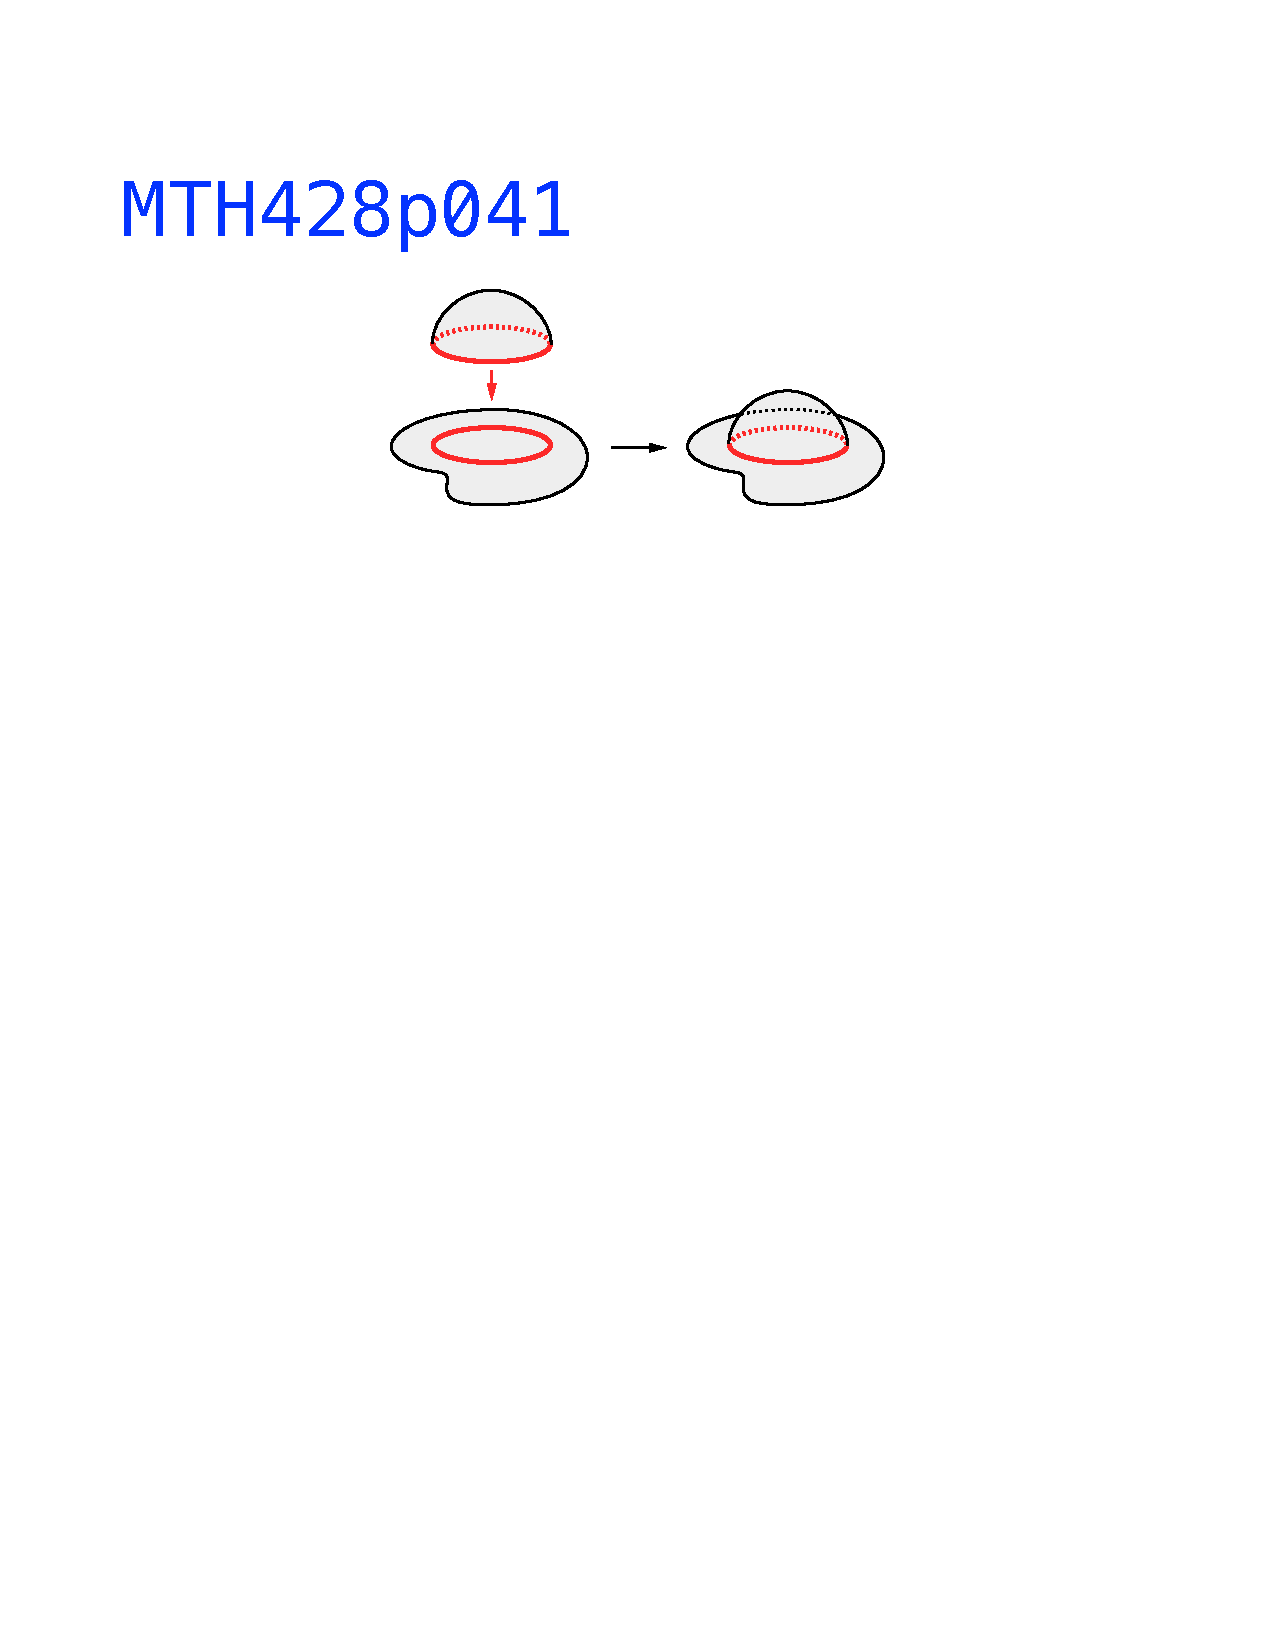
\includegraphics[width=\textwidth, trim=0mm 192mm 0mm 49mm, clip]{pictures/MTH427p012.pdf}}};

%%% COORDINATE GRID
%\draw[step=0.5, help lines] (0,0) to[grid with coordinates] (15,9);
%%% 

\node[anchor=  base]  at (6.7 , 1.6){\color{red} \small  $f$};
\node[anchor=  east]  at (5.6 , 2.5){ \small  $D^{n}$};
\node[anchor=  east]  at (5.0 , 1.0){ \small  $X$};
\node[anchor=  west]  at (11.5 , 1.0){ \small  $X\cup_{f}D^{n}$};
\end{tikzpicture}
\end{equation*}
\end{exercise}

Show that if $X$ is a normal space then the space $X\cup_{f} D^{n}$ is normal. 







\newpage
%%%%%%%%%%%%%%%%%%%%%%%%%%%%%%%
%%%%%%%%%%%%%%%%%%%%%%%%%%%%%%%
%%%
%%%  SIMPLICIAL COMPLEXES
%%%
%%%%%%%%%%%%%%%%%%%%%%%%%%%%%%%
%%%%%%%%%%%%%%%%%%%%%%%%%%%%%%%

%---BBLANK #
\chapter[Simplicial Complexes]{Simplicial\\ Complexes}
%---EBLANK #
\chaptermark{Simplicial Complexes}

\thispagestyle{firststyle}
\label{SIMPLICIAL COMPLEXES CH}


The straightforward way of constructing  a topological space is to describe its sets of points 
and the collection of open sets. Many constructions in geometry and topology, however, take 
a less direct approach. They specify a collection of simple topological spaces that serve as 
building blocks. Then, in order to construct more complex spaces, one just needs to  give a 
recipe how these building blocks should be put together. Simplicial complexes introduced in this 
chapter are one example of such framework, but there are several others: cubical complexes, 
simplicial sets, CW-complexes etc.  These constructions differ in the selection of spaces which
serve as the building blocks, how ``recipes'' for assembling these building blocks look like, and how 
the building process is conducted. 

%---BBLANK # \vskip 40mm
\begin{definition}
\label{SIMPL COMPLEX DEF}
A \emph{simplicial complex} $K = (V, S)$ consists of a set $V$ together with a set 
$S$ of finite, non-empty subsets of $V$ such that the following conditions are satisfied:
\benu
\item[1)] For each $v\in V$ the set $\{v\}$  is in $S$. 
\item[2)] If $\sigma \in S$ and $\varnothing \neq \tau \subseteq \sigma$ then $\tau \in S$. 
\eenu
\end{definition}
%---EBLANK #

%---BBLANK # \newpage
\begin{notation}
If $K= (V, S)$ is a simplicial complex then:
\benu[leftmargin = *]
\item[\textbullet] Elements of $V$ are called \emph{vertices} of $K$.
\item[\textbullet] Elements of $S$ are called \emph{simplices} of $K$. 
\item[\textbullet] If  a simplex $\sigma\in S$ consists of $n+1$ elements then 
we say that $\sigma$ is  an \emph{$n$-simplex}. 
\item[\textbullet]  If  $\sigma\in S$  and $\tau\subseteq \sigma$ then we say that 
$\tau$ is a \emph{face} of $\sigma$. If $\tau \neq \sigma$ then $\tau$ is a \emph{proper face} of 
$\sigma$. The inclusion $j^{\sigma}_{\tau}\colon \tau \to \sigma$ is called 
a \emph{face map}.
\item[\textbullet] We say that $K$ is a simplicial complex of dimension $n$ if $K$ has $n$-simplices,
but it does not have m-simplices for $m>n$. We write: $\dim K = n$. If $K$ has simplices in all dimensions 
then $\dim K = \infty$. 
\item[\textbullet]  We say that $K$ is a finite simplicial complex if $K$ consists of finitely many simplices. 
\eenu
\end{notation}
%---EBLANK #


We will write $\sigma \in K$ to denote that $\sigma$ is a simplex of $K$. 


\begin{example}
If $\Gamma$ is a  graph then 
then we can define a simplicial complex $K(\Gamma)$ whose vertices are vertices of $\Gamma$, 
and whose 1-simplices are  sets $\{v_{1}, v_{2}\}$ such that there is an edge  of $\Gamma$ that joins 
$v_{1}$ with $v_{2}$.  The complex $K(\Gamma)$ has no simplices in dimensions greater than 1. 
\end{example}
 

\begin{example}
\label{NERVE EXAMPLE}
Let $X$ be a set, and let $\mathcal{A} = \{A_{i}\}_{i\in I}$ be a collection of subsets of $X$. 
The \emph{nerve} of $\mathcal{A}$ is the simplicial complex $N(\mathcal{A})$ whose  vertices are elements of 
$\mathcal{A}$. A set $\{A_{i_{0}}, \dots, A_{i_{n}}\}$ is a simplex in $N(\mathcal{A})$ if
$A_{i_{1}}\cap {\dots} \cap A_{i_{n}} \neq \varnothing$. 
\end{example}

\begin{example}
\label{CECH COMPLEX EXAMPLE}
As a special case of the construction of a nerve (\ref{NERVE EXAMPLE}), let $(X, \varrho)$ be a metric space,
and for a fixed  $\varepsilon > 0$ let $\mathcal{B}_{\varepsilon}$ be the collection of all open ball in $X$ of radius 
$\varepsilon$: 
$$\mathcal{B}_{\varepsilon} = \{ B(x, \varepsilon) \ | \ x\in X\}$$
The nerve $N(\mathcal{B}_{\varepsilon})$ is called the \emph{\v{C}ech complex} of $X$ and it is  denoted 
$\check{C}(X, \varepsilon)$. 
\end{example}


%---BBLANK # \newpage
\begin{definition}
If $K = (V, S)$ is a simplicial complex, then a \emph{subcomplex} of $K$ is a simplicial complex 
$L = (V', S')$ such that $V'\subseteq V$ and $S'\subseteq S$. In such case we write $L \subseteq K$. 
\end{definition}
%---EBLANK #

\begin{example}
\label{SIMPLEX SUBCOMPLEX EXAMPLE}
A simplex $\sigma$  of a simplicial complex $K$ defines a subcomplex $\xov\sigma \subseteq K$ consisting 
of all faces of $\sigma$ and a subcomplex $\partial \sigma \subseteq K$ consisting of all proper 
faces of $\sigma$. 
\end{example}




We will show that every simplicial complex $K$ defines a certain topological space $|K|$. 
This space is assembled from  building blocks given by geometric simplices.  The structure  of $K$ 
provides a blueprint how the assembly process should be performed. 


%---BBLANK # \vskip 70mm
\begin{definition}
Let  
$e_{1} = (1, 0, 0, \dots, 0), \ e_{2} = (0, 1, 0, \dots, 0), \dots, \ e_{n+1} = (0, 0, 0, \dots, 1)$ be the 
standard basis vectors in $\R^{n+1}$. 
The \emph{standard geometric $n$-simplex} is a subspace $\Delta^{n} \subseteq \R^{n+1}$ given by 
\begin{align*}
\Delta^{n} 
& = \left\{ \sum_{i=1}^{n+1} t_{i}e_{i} \in \R^{n+1} \ | \  t_{i}\in [0, 1], \ \textstyle{\sum^{n}_{i=0} t_{i}} = 1\right\}        
\end{align*}
\end{definition}

%vskip -10mm

\tdplotsetmaincoords{66}{45}
\begin{equation*}
\begin{tikzpicture}[scale = 1] 
\begin{scope}
\draw[->, >=latex, thick] (-0.5,0) -- (2, 0);
\draw[line width = 1pt, red, fill=red, text = black] (1.5, 0) circle (0.1) 
node[below, yshift = -2pt, xshift = 1pt] {\small $e_{1}$}
node[red, above,  yshift = 4pt, xshift = 4pt] {$\Delta^{0}$};
\end{scope}
\begin{scope}[xshift = 40mm]
\draw[->, >=latex, thick] (-0.5,0) -- (2, 0);
\draw[->, >=latex, thick] (0, -0.5) -- (0, 2.0);
\draw[line width = 1pt, red, fill=red, text = black] (1.5, 0) circle (0.1) node[below, yshift = -2pt, xshift = 1pt] {\small $e_{1}$};
\draw[line width = 1pt, red, fill=red, text = black] (0, 1.5) circle (0.1) node[left, xshift = -2pt] {\small $e_{2}$};
\draw[line width = 2pt, red] (1.5, 0) -- (0, 1.5) node[pos=0.5, red, anchor = south west] {$\Delta^{1}$};
\end{scope}
\begin{scope}[xshift = 80mm]
\draw[->, >=latex, thick] (-0.5,{-0.5/3}) -- (2, 2/3);
\draw[->, >=latex, thick] (0, -0.5) -- (0, 2.0);
\draw[->, >=latex, thick] (-0.5, {0.5/3}) -- (1.5, -0.5);
\draw[line width = 1pt, red, fill=red, text = black] 
(1.5, 0.5) circle (0.1) node[below, yshift = -3pt, xshift = 6pt] {\small $e_{1}$};
\draw[line width = 1pt, red, fill=red, text = black] 
(0, 1.5) circle (0.1) node[left, xshift = -2pt] {\small $e_{3}$};
\draw[line width = 1pt, red, fill=red, text = black] 
(1, -1/3) circle (0.1) node[below, xshift = 0pt, yshift = -3pt] {\small $e_{2}$};
\draw[line width = 2pt, red, fill=mypink, fill opacity = 0.7] (1.5, 0.5) -- (0, 1.5) -- (1, -1/3) -- cycle; 
\node[anchor = south west, red] at (0.95, 0.95) {$\Delta^{2}$};
\end{scope}

\begin{scope}[xshift = 120mm, yshift = 2.4mm,    
                             scale = 2, 
                             tdplot_main_coords,
                             line join = round, 
                             line cap = round,
                             line1/.style = {line width = 2pt, red, fill=mypink},
                             ]
                             
\pgfmathsetmacro{\sqthree}{sqrt(3)};
\pgfmathsetmacro{\sqsix}{sqrt(6)};
\coordinate (A) at (0,0,0);
\coordinate (B) at (1,0,0);
\coordinate (C) at (0.5, \sqthree/2, 0);
\coordinate (D) at (0.5, \sqthree/6, \sqsix/3);

\draw[line1, opacity=.4] (A)--(B)--(C)--cycle;
\draw[line1,  opacity=.4] (A) --(D)--(C)--cycle;
\draw[line1, fill opacity=.6] (B)--(D)--(C)--cycle;
\draw[line1, fill opacity=.6] (A)--(D)--(B)--cycle;

\tdplottransformmainscreen{0}{0}{0}
\draw[tdplot_screen_coords, line width = 1pt, red, fill=red, text = black]  
(\tdplotresx,\tdplotresy) circle (0.05) node[below, yshift = -1pt, xshift = -7pt] {\small $e_{1}$};
\tdplottransformmainscreen{1}{0}{0}
\draw[tdplot_screen_coords, line width = 1pt, red, fill=red, text = black]  
(\tdplotresx,\tdplotresy) circle (0.05) node[below, yshift = -3pt, xshift = 4pt] {\small $e_{2}$};
\tdplottransformmainscreen{0.5}{\sqthree/2}{0}
\draw[tdplot_screen_coords, line width = 1pt, red, fill=red, text = black]  
(\tdplotresx,\tdplotresy) circle (0.05) node[below, yshift = 2pt, xshift = 12pt] {\small $e_{3}$};
\tdplottransformmainscreen{0.5}{\sqthree/6}{\sqsix/3}
\draw[tdplot_screen_coords, line width = 1pt, red, fill=red, text = black]  
(\tdplotresx,\tdplotresy) circle (0.05) node[above, yshift = 3pt, xshift = 2pt] {\small $e_{4}$};
\tdplottransformmainscreen{1}{0.35}{0.8}
\node[tdplot_screen_coords, red] at (\tdplotresx,\tdplotresy) {\small $\Delta^{3}$};
\end{scope}

\end{tikzpicture}
\end{equation*}
%---EBLANK #


By the above definition vertices of the standard geometric simplex $\Delta^{n}$ correspond to the vectors 
$e_{1}, \dots, e_{n+1}$. It will be useful to modify this construction, so that vertices of a geometric simplex 
can be indexed by elements of any given finite set:


%---BBLANK # \newpage
\begin{definition}
Let $A$ be a finite set.  The \emph{geometric $A$-simplex} is a metric space 
$(\Delta^{A}, \varrho)$, such that elements of $\Delta^{A}$ are  formal sums $\sum_{a\in A} t_{a}a$  where
$t_{a}\in [0,1]$ for each $a\in A$, and $\sum_{a\in A} t_{a} = 1$. If $x = \sum_{a\in A} t_{a}a$  and 
$y = \sum_{a\in A} t'_{a}a$ then 
$$\varrho(x, y) = \textstyle{\sqrt{\sum_{a\in A} (t_{a} - t'_{a})^{2}}}$$
\end{definition}
%---EBLANK #

%---BBLANK # \vskip 40mm
\begin{proposition}
If $A$ is a set consisting of $n+1$ elements then $\Delta^{A}$ is homeomorphic to the standard $n$-simplex 
$\Delta^{n}$. 
\end{proposition}

\begin{proof}
Exercise. 
\end{proof}
%---EBLANK #


If $A$ is a finite set and $B\subseteq A$, then the simplex $\Delta^{B}$ is a subspace of $\Delta^{A}$
and the inclusion map $j\colon B \to A$ induces  a continuous inclusion $\Delta(j)\colon \Delta^{B} \to \Delta^{A}$.
We will say that $\Delta^{B}$ is a \emph{face} of $\Delta^{A}$. If $B\neq A$ then it is a \emph{proper face}. 

\begin{equation*}
\begin{tikzpicture}[scale = 1.8,
                              line1/.style ={line width = 1.5pt, fill=mygray2},
                             ]
\coordinate (a) at (0:0); 
\coordinate (b) at (0:1);
\coordinate (c) at (60:1);
\coordinate (shift) at (2, 0);

\coordinate (aa) at ($(a) - (shift)$);
\coordinate (cc) at  ($(c) - (shift)$);
\draw[line1] (a) -- (b) -- (c) -- cycle;
\draw[line1] (aa) -- (cc);
\fill (a) circle (0.05) node[anchor = base, yshift = -12pt] {\small $a$};
\fill (b) circle (0.05) node[anchor = base, yshift = -12pt] {\small $b$};
\fill (c) circle (0.05) node[anchor = base, yshift = 6pt] {\small $c$};
\fill (aa) circle (0.05) node[anchor = base, yshift = -12pt] {\small $a$};
\fill (cc) circle (0.05) node[anchor = base, yshift = 6pt] {\small $c$};
\draw[->, >=latex, line width = 1pt] (-1.2,0.43) -- (-0.2, 0.43) node[above, pos = 0.5] {\small $\Delta(j)$}; 
\end{tikzpicture}
\end{equation*}

In particular, if $\sigma$ is a simplex of a simplicial complex $K$, and $\tau$ is a face of $\sigma$
then the face map $j^{\sigma}_{\tau}\colon \tau\to \sigma$ defines a map 
$\Delta(j^{\sigma}_{\tau}) \colon \Delta^{\tau} \to \Delta^{\sigma}$.  


%---BBLANK # \newpage
\begin{definition}
Let $K$ be a simplicial complex. The \emph{geometric realization} of $K$ is the topological space 
$|K|$ defined by:
$$|K| = \quotient{\bigsqcup_{\sigma\in K} \Delta^{\sigma}}{\sim}$$

where the equivalence relation $\sim$ is given by $x\sim \Delta(j^{\sigma}_{\tau})(x)$ for each face 
map $j^{\sigma}_{\tau}\colon \tau\to \sigma$ and $x\in \Delta^{\tau}$. 
\end{definition}
%---EBLANK #

\begin{example}
Let $K$ be a simplicial complex with vertices $\{a, b, c, d, e\}$ and simplices 
$\{a, b, c\}$, $\{a, b, d\}$, $\{a, b\}$, $\{a, c\}$, $\{b, c\}$, $\{a, d\}$, $\{b, d\}$, $\{a, e\}$, $\{a\}$, $\{b\}$, $\{c\}$, 
$\{d\}$, $\{e\}$.  The picture on the left shows the disjoint union $\bigsqcup_{\sigma\in K} \Delta^{\sigma}$, and 
the picture on the right shows the geometric realization $|K|$:


\begin{equation*}
\begin{tikzpicture}[
                              scale = 1.35 ,
                              line1/.style ={line width = 1.5pt, fill=mygray2},
                              line2/.style ={line width = 1pt, fill=mygray2},
                              ] 
                              

%left picture
\begin{scope}
\coordinate (a) at (0:0); 
\coordinate (b) at (0:1);
\coordinate (c) at (60:1);
\coordinate (d) at (-60:1);
\coordinate (e) at (180:1);

\coordinate (su) at (90:0.35);
\coordinate(sleft) at (30:0.35);
\coordinate(sright) at (150:0.35);
\coordinate(sleftd) at (-30:0.35);
\coordinate(srightd) at (210:0.35);

\coordinate (aur) at ($(a) + (sright) + (su)$);
\coordinate (cur) at ($(c) + (sright) + (su)$);
\coordinate (bur) at ($(b) + (sright) + (su)$);

\coordinate (aul) at ($(a) + (sleft) + (su)$);
\coordinate (cul) at ($(c) + (sleft) + (su)$);
\coordinate (bul) at ($(b) + (sleft) + (su)$);

\coordinate (adr) at ($(a) + (srightd) - (su)$);
\coordinate (bdr) at ($(b) + (srightd) - (su)$);
\coordinate (ddr) at ($(d) + (srightd) - (su)$);

\coordinate (adl) at ($(a) + (sleftd) - (su)$);
\coordinate (bdl) at ($(b) + (sleftd) - (su)$);
\coordinate (ddl) at ($(d) + (sleftd) - (su)$);

\path[name path = ulpath]  ($(cul)!2!(bul)$) -- ($(bul)!2!(cul)$);
\path[name path = urpath]  ($(aur)!2!(cur)$) -- ($(cur)!2!(aur)$);
\path [name intersections={of=ulpath and urpath , by={top}}];

\path[name path = dlpath]  ($(bdl)!2!(ddl)$) -- ($(ddl)!2!(bdl)$);
\path[name path = drpath]  ($(adr)!2!(ddr)$) -- ($(ddr)!2!(adr)$);
\path [name intersections={of=dlpath and drpath , by={bottom}}];

\path [name intersections={of=ulpath and dlpath , by={left}}];
\path [name intersections={of=urpath and drpath , by={right}}];

\draw[line2] ($(a) + (su)$) -- ($(b) + (su)$) -- ($(c) + (su)$)  -- cycle;
\draw[line2] ($(a) - (su)$) -- ($(b) - (su)$) -- ($(d) - (su)$)  -- cycle;
\draw[line1] (a) -- (b);
\

\draw[line1]  (bul) --  node[above, sloped] {\small $bc$} (cul);
\draw[line1]  (aur) --  node[above, sloped] {\small $ac$} (cur);
\draw[line1]  (adr) --  node[below, sloped] {\small $ad$} (ddr);
\draw[line1]  (bdl) --  node[below, sloped] {\small $bd$} (ddl);
\node at ($(30:0.58)+(su)$) {\small $abc$}; 
\node at ($(-30:0.58)-(su)$) {\small $abd$}; 
\node[above] at (0:0.5) {\small $ab$}; 

\fill[] (top) circle (0.05) node[above, yshift =3pt, yshift =1pt] {\small $c$};
\fill[] (bottom) circle (0.05) node[below, yshift =-4pt, yshift =0pt] {\small $d$};
\fill[] (left) circle (0.05) node[above, yshift =3pt, yshift =1pt] {\small $b$};
\fill[] (right) circle (0.05) node[above, yshift =3pt, yshift =1pt] {\small $a$};
\fill[] ($(left)!2!(right)$) circle (0.05) node[above, yshift =3pt, yshift =1pt] {\small $e$};
\draw[line1] ($(a)!2!(right)$) --  node[above, sloped] {\small $ae$} ($(b)!2!(right)$);
\end{scope}

%arrow
\begin{scope}[xshift = 28mm]
\draw[->, >=latex, line width = 1pt] (0, 0) -- (0.7,0); 
\end{scope}

%right picture
\begin{scope}[xshift = 55mm]
\coordinate (a) at (0:0); 
\coordinate (b) at (0:1);
\coordinate (c) at (60:1);
\coordinate (d) at (-60:1);
\coordinate (e) at (180:1);
\draw[line1] (a) -- (b) -- (c) -- cycle ;
\draw[line1] (a) -- (b) -- (d) -- cycle; 
\draw[line1] (a) -- (e);
\foreach \point in {(a), (b), (c), (d), (e)} {\fill \point circle (0.05);}
\end{scope}


\end{tikzpicture}
\end{equation*}
\end{example}
The following fact will be useful later on:


%---BBLANK # \vfill
\begin{proposition} 
\label{SUBCOMPLEX REALZATION PROP}
If  $L$ is a subcomplex of a simplicial complex $K$, then $|L|$ is a closed subspace of $|K|$. 
\end{proposition}

\begin{proof}
Exercise. 
\end{proof}
%---EBLANK #

Simplicial complexes and their geometric realizations are very useful tools, because they are a source of 
algebraic invariants of topological spaces. We will illustrate this using an example of one such invariant, 
the Euler characteristic.


%---BBLANK # \newpage
\begin{definition}
Let $K$ be a finite simplicial complex. For $n=0, 1, 2, \dots$ let $s_{n}(K)$ denote the number of $n$-simplices
of $K$. The \emph{Euler characteristic} of $K$ is the integer 
$$\chi(K) = \sum_{n=0}^{\infty} (-1)^{n}s_{n}(K)$$ 
\end{definition}
%---EBLANK #

The following fact is one of the most important properties of the Euler characteristic. We will omit its proof. 

%---BBLANK # \vskip 40mm
\begin{theorem}
\label{SIMPLICIAL EULER CHAR INVARIANCE  THM}
If $K$, $L$ are finite simplicial complexes such that $|K|$ is homeomorphic to $|L|$ then $\chi(K) = \chi(L)$. 
\end{theorem}
%---EBLANK #

\begin{example}
For $n\geq 3$ let $K_{n}$ be a simplicial complex of dimension 1 whose set of vertices is $\{a_{1}, \dots, a_{n}\}$, and
whose 1-simplices are sets $\{a_{i}, a_{i+1}\}$ for $1\leq i \leq n-1$ and $\{a_{n}, a_{1}\}$. Notice that  each 
space $|K_{n}|$ is homeomorphic to the circle $S^{1}$:

%---BBLANK # \vskip 20mm
\begin{equation*}
\begin{tikzpicture}[
                              scale = 1.6 ,
                              line1/.style ={line width = 1.5pt},
                              line2/.style ={line width = 1pt},
                              ] 
                              
\begin{scope}[scale = 1]
\pgfmathsetmacro{\myrad}{1/(sin(90) - sin(-30))};
\coordinate (o) at (0, 0); 
\coordinate (a) at (-30:\myrad); 
\coordinate (b) at ($(90:\myrad)-(a)$); 
\coordinate (c) at ($(210:\myrad)-(a)$); 
\draw[line1] (o) -- (b) -- (c) -- node[below, yshift = -10pt] {\small $|K_{3}|$}  cycle ; 
\foreach \point in {(o), (b), (c)} {\fill \point circle (0.06);}
\end{scope}

\begin{scope}[scale = 1, xshift = 20mm]
\pgfmathsetmacro{\myrad}{1/(sin(45) - sin(-45))};
\coordinate (o) at (0, 0); 
\coordinate (a) at (-45:\myrad); 
\coordinate (b) at ($(45:\myrad) - (a)$); 
\coordinate (c) at ($(135:\myrad) - (a)$); 
\coordinate (d) at ($(225:\myrad) - (a)$); 
\draw[line1] (o) -- (b) -- (c) -- (d)  --  cycle; 
\path (d) -- node[below, yshift = -10pt] {\small $|K_{4}|$} (o); 
\foreach \point in {(o), (b), (c), (d)} {\fill \point circle (0.06);}
\end{scope}

\begin{scope}[xshift = 40mm]
\pgfmathsetmacro{\myrad}{1/(sin(90) - sin(-54))};
\coordinate (o) at (0, 0); 
\coordinate (a) at (-54:\myrad); 
\coordinate (b) at ($(18:\myrad) - (a)$); 
\coordinate (c) at ($(90:\myrad) - (a)$); 
\coordinate (d) at ($(162:\myrad) - (a)$); 
\coordinate (e) at ($(234:\myrad) - (a)$); 
\draw[line1] (o) -- (b) -- (c) -- (d) -- (e) -- cycle; 
\path (e) -- node[below, yshift = -10pt] {\small $|K_{5}|$} (o); 
\foreach \point in {(o), (b), (c), (d), (e)} {\fill \point circle (0.06);}
\end{scope}

\begin{scope}[xshift = 60mm]
\pgfmathsetmacro{\myrad}{1/(sin(60) - sin(-60))};
\coordinate (o) at (0, 0); 
\coordinate (a) at (-60:\myrad); 
\coordinate (b) at ($(0:\myrad) - (a)$); 
\coordinate (c) at ($(60:\myrad) - (a)$); 
\coordinate (d) at ($(120:\myrad) - (a)$); 
\coordinate (e) at ($(180:\myrad) - (a)$); 
\coordinate (f) at ($(240:\myrad) - (a)$); 
\draw[line1] (o) -- (b) -- (c) -- (d) -- (e) -- (f) -- cycle; 
\path (f) -- node[below, yshift = -10pt] {\small $|K_{6}|$} (o); 
\foreach \point in {(o), (b), (c), (d), (e), (f)} {\fill \point circle (0.06);}
\end{scope}

\end{tikzpicture}
\end{equation*}
%---EBLANK #

Since in each complex $K_{n}$ the  number of $0$-simplices is the same as the number of $1$-simplices,  
we have $\chi(K_{n}) = 0$ for any $n\geq 3$. 

\end{example}

We can extend the notion of the Euler characteristic to the realm of topological spaces as follows:

%---BBLANK # \newpage
\begin{definition}
If $X$ is a topological space such that $X\cong |K|$ for some finite simplicial complex $K$ then  we define
the Euler characteristic $\chi(X)$ of $X$ as the Euler characteristic $\chi(K)$ of $K$. 
\end{definition}
%---EBLANK #

Notice that by Theorem \ref{SIMPLICIAL EULER CHAR INVARIANCE  THM} 
the Euler characteristic of a space $X$
is a well defined. Indeed, if $X\cong |K|$ and $X\cong |L|$ for some finite simplicial complexes
$K$ and $L$ then $|K|\cong |L|$, and so $\chi(K) = \chi(L)$. Therefore the value of $\chi(X)$ does not depend
on the choice of  a simplicial complex $K$ such that $X\cong |K|$. Moreover, we have:

%---BBLANK # \vskip 60mm
\begin{proposition}
\label{TOP EULER CHAR INVARIANCE  THM}
The Euler characteristic is a topological invariant: if $X$, $Y$ are spaces such that $X\cong Y$ and 
$\chi(X)$ is defined, then $\chi(Y)$ is defined and $\chi(Y) = \chi(X)$.
\end{proposition}
%---EBLANK #


\begin{proof}
If $\chi(X)$ is defined then $X \cong |K|$ for some finite simplicial complex $K$. Then 
$Y\cong X \cong |K|$, and so $\chi(Y) = \chi(K) = \chi(X)$. 
\end{proof}

%---BBLANK # \newpage
\begin{example}
\label{EULER CHAR S2 TORUS EXAMPLE}
We will use the Euler characteristic to show that the 2-dimensional sphere $S^{2}$ is not homeomorphic to the 
torus $T = S^{1}\times S^{1}$. 
%---EBLANK # \end{example}

The sphere $S^{2}$ is homeomorphic to the surface of the tetrahedron:

\begin{equation*}
\tdplotsetmaincoords{66}{45}
\begin{tikzpicture}[
                             scale = 2.5, 
                             tdplot_main_coords,
                             line join = round, 
                             line cap = round,
                             line1/.style = {line width = 1.5pt},
                             ]
                             
\pgfmathsetmacro{\sqthree}{sqrt(3)};
\pgfmathsetmacro{\sqsix}{sqrt(6)};
\coordinate  (shift) at (0, 0, 0);
\coordinate (A) at ($(0,0,0) + (shift)$);
\coordinate (B) at ($(1,0,0) + (shift)$);
\coordinate (C) at ($(0.5, \sqthree/2, 0) + (shift)$);
\coordinate (D) at ($(0.5, \sqthree/6, \sqsix/3) + (shift)$);

\draw[line1, opacity=.4] (A)--(B)--(C)--cycle;
\draw[line1, fill=mygray2, fill opacity=.3] (A) --(D)--(C)--cycle;
\draw[line1, fill=mygray2, fill opacity=.7] (B)--(D)--(C)--cycle;
\draw[line1, fill=mygray2, fill opacity=.7] (A)--(D)--(B)--cycle;

\end{tikzpicture}
\end{equation*}

This surface can be obtained as a geometric realization of a simplicial complex which has 4 $0$-simplices, 
6 $1$-simplices and $4$ $2$-simplices. This gives: $\chi(S^{2}) = 4-6+4 = 2$.  

Next, recall that the torus $T$ can be constructed by identifying edges of a square:

{{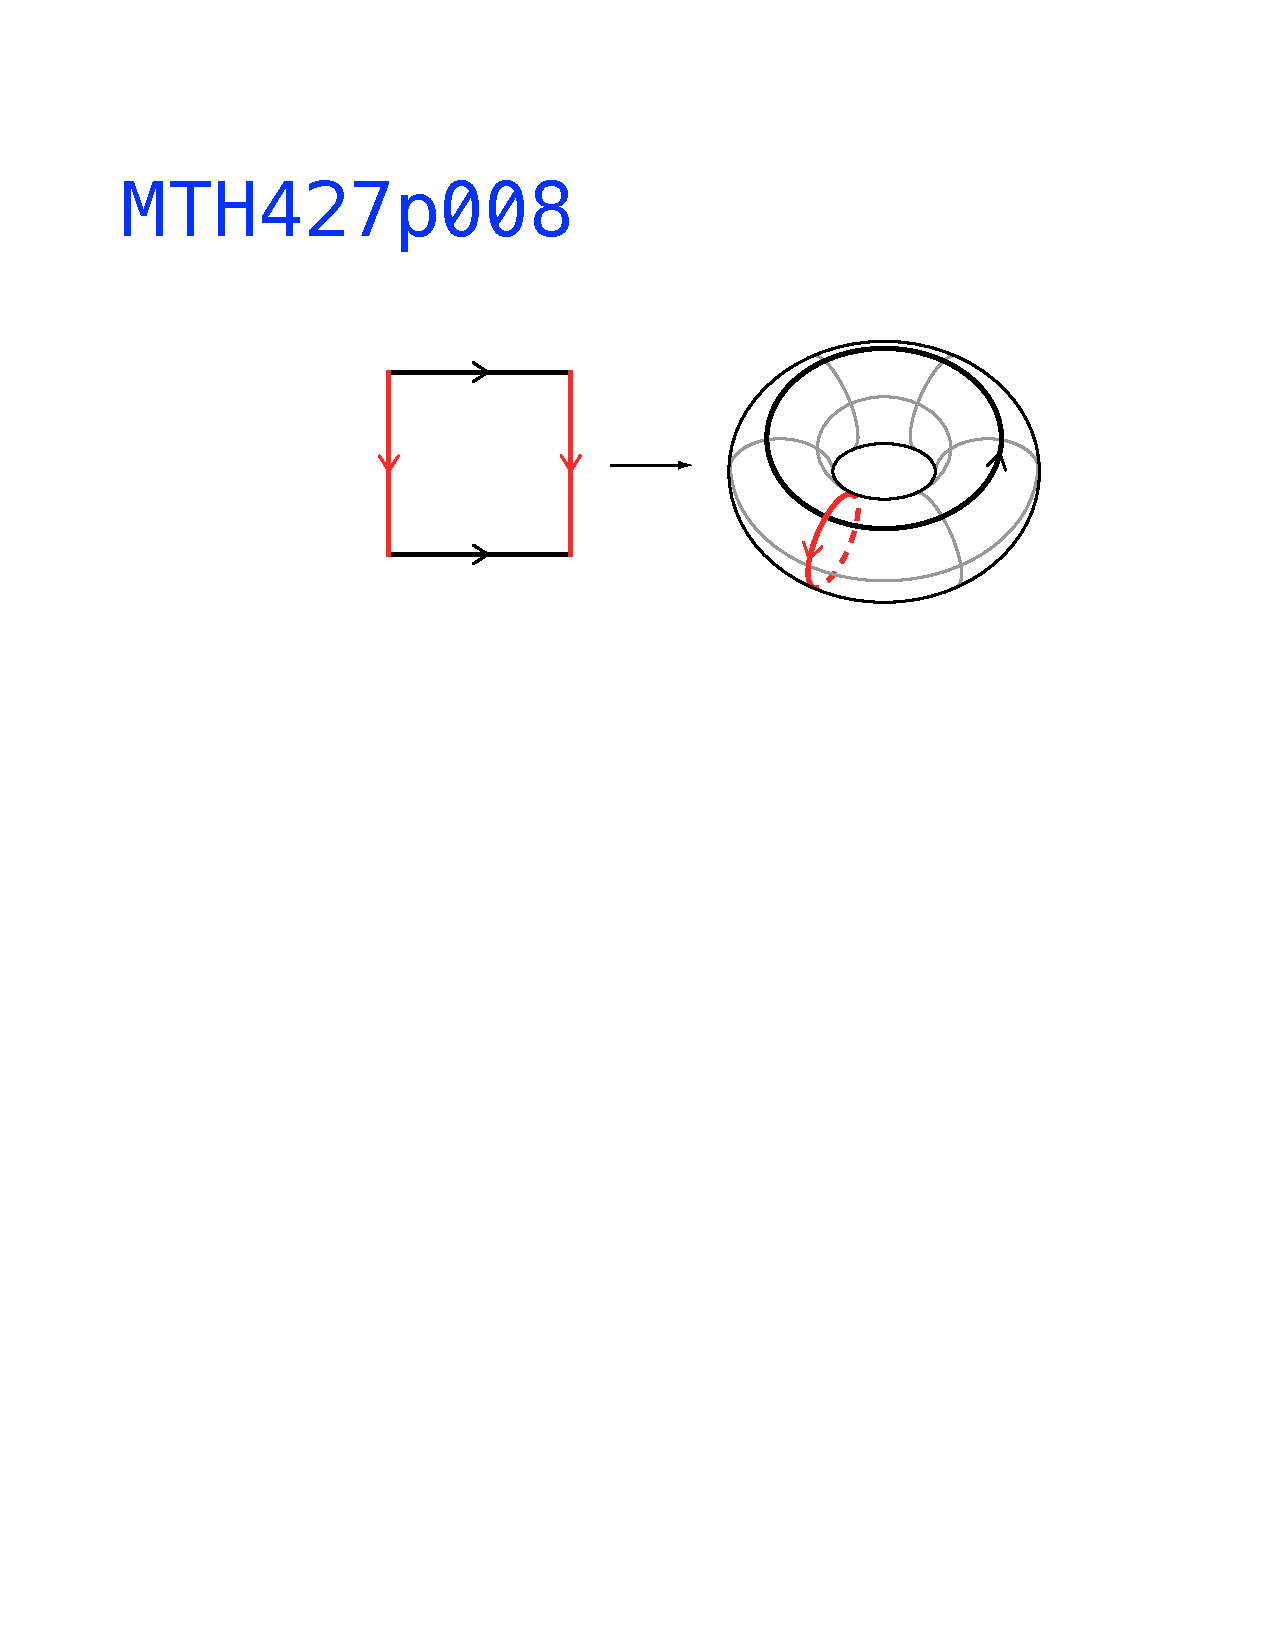
\includegraphics[width=\textwidth, trim=0mm 176mm 0mm 57mm, clip]{pictures/MTH427p008.pdf}}   }

Subdividing the square we can represent the torus as a geometric realization of a simplicial complex:

\begin{equation*}
\begin{tikzpicture}[
                             scale = 1,
                             line1/.style = {line width = 1.5pt}
                             ]
                                             
\draw[line1] (0, 0) rectangle (3, 3);
\draw[line1] (0, 1) -- (3, 1);
\draw[line1] (0, 2) -- (3, 2);
\draw[line1] (1, 0) -- (1, 3);
\draw[line1] (2, 0) -- (2, 3);

\draw[line1] (0, 2) -- (1, 3);
\draw[line1] (0, 1) -- (2, 3);
\draw[line1] (0, 0) -- (3, 3);
\draw[line1] (1, 0) -- (3, 2);
\draw[line1] (2, 0) -- (3, 1);
\node[anchor = base, yshift = -12pt, xshift = -8pt] at (0, 0) {\small $a$}; 
\node[anchor = base, yshift = -12pt, xshift = 0pt] at (1, 0) {\small $b$}; 
\node[anchor = base, yshift = -12pt, xshift = 0pt] at (2, 0) {\small $c$}; 
\node[anchor = base, yshift = -12pt, xshift = 8pt] at (3, 0) {\small $a$}; 

\node[anchor = base, yshift = 6pt, xshift = -8pt] at (0, 3) {\small $a$}; 
\node[anchor = base, yshift = 6pt, xshift = 0pt] at (1, 3) {\small $b$}; 
\node[anchor = base, yshift = 6pt, xshift = 0pt] at (2, 3) {\small $c$}; 
\node[anchor = base, yshift = 6pt, xshift = 8pt] at (3, 3) {\small $a$}; 


\node[anchor = base, yshift = 0pt, xshift = -8pt] at (0, 2) {\small $d$}; 
\node[anchor = base, yshift = 0pt, xshift = 8pt] at (3, 2) {\small $d$}; 
\node[anchor = base, yshift = 0pt, xshift = -8pt] at (0, 1) {\small $e$}; 
\node[anchor = base, yshift = 0pt, xshift = 8pt] at (3, 1) {\small $e$}; 

\node[anchor = north west] at (1, 1) {\small $f$}; 
\node[anchor = north west] at (2, 1) {\small $g$}; 
\node[anchor = north west] at (1, 2) {\small $h$}; 
\node[anchor = north west] at (2, 2) {\small $i$}; 
\end{tikzpicture}
\end{equation*}

This simplicial complex has 9 0-simplices, 27 1-simplices, and 18 2-simplices. This gives 
$\chi(T) = 9 - 27 + 18 = 0$.  Since $\chi(T) \neq \chi(S^{2})$  by 
Proposition \ref{SIMPLICIAL EULER CHAR INVARIANCE  THM}
we obtain that $T\not\cong S^{2}$. 
\end{example}

%---BBLANK # \newpage {\bf Topological  data analysis.}
%---EBLANK # 
\begin{TDA NN}
While simplicial complexes have been known and studied for a long time, more recently they 
appeared in the field of topological data analysis (TDA), which uses topological 
methods to study sets of data. The premise of TDA is that a set of data can be considered as  
a sample of points taken from some underlying, unknown topological space $X$, and that properties 
of that underlying space  (its number of connected  components,  the Euler characteristic etc.) provide 
an insight into the data.  

%---BBLANK # \vskip 20mm
\begin{equation*}
\begin{tikzpicture}[scale=0.65,
                              line1/.style = {red},
                             ]
                             
\begin{scope}
\fill[line1] (1.0, 1.0) circle (0.06);
\fill[line1] (3.0, 1.0) circle (0.06);
\fill[line1] (4.0, 1.2) circle (0.06);
\fill[line1] (3.2, 0.8) circle (0.06);
\fill[line1] (3.4, 1.6) circle (0.06);
\fill[line1] (3.4, 3.0) circle (0.06);
\fill[line1] (3.6, 0.8) circle (0.06);
\fill[line1] (3.6, 2.2) circle (0.06);
\fill[line1] (4.0, 2.0) circle (0.06);
\fill[line1] (4.2, 1.4) circle (0.06);
\fill[line1] (3.6, 1.4) circle (0.06);
\fill[line1] (3.8, 2.6) circle (0.06);
\fill[line1] (4.2, 1.8) circle (0.06);
\fill[line1] (4.2, 2.4) circle (0.06);
\fill[line1] (3.6, 1.6) circle (0.06);
\fill[line1] (3.6, 0.6) circle (0.06);
\fill[line1] (3.4, 2.6) circle (0.06);
\fill[line1] (3.4, 0.6) circle (0.06);
\fill[line1] (3.4, 2.4) circle (0.06);
\fill[line1] (3.2, 0.4) circle (0.06);
\fill[line1] (3.2, 1.2) circle (0.06);
\fill[line1] (3.2, 2.0) circle (0.06);
\fill[line1] (3.2, 2.6) circle (0.06);
\fill[line1] (3.0, 0.4) circle (0.06);
\fill[line1] (3.0, 0.6) circle (0.06);
\fill[line1] (3.0, 2.4) circle (0.06);
\fill[line1] (3.0, 2.8) circle (0.06);
\fill[line1] (3.0, 3.2) circle (0.06);
\fill[line1] (2.8, 1.0) circle (0.06);
\fill[line1] (2.8, 2.8) circle (0.06);
\fill[line1] (2.8, 3.0) circle (0.06);
\fill[line1] (2.6, 0.2) circle (0.06);
\fill[line1] (2.6, 0.4) circle (0.06);
\fill[line1] (2.6, 0.8) circle (0.06);
\fill[line1] (2.6, 0.2) circle (0.06);
\fill[line1] (2.4, 0.2) circle (0.06);
\fill[line1] (2.4, 0.6) circle (0.06);
\fill[line1] (2.4, 3.0) circle (0.06);
\fill[line1] (2.4, 3.2) circle (0.06);
\fill[line1] (2.2, 0.6) circle (0.06);
\fill[line1] (2.2, 3.4) circle (0.06);
\fill[line1] (2.2, 3.2) circle (0.06);
\fill[line1] (2.0, 0.2) circle (0.06);
\fill[line1] (2.0, 0.4) circle (0.06);
\fill[line1] (2.0, 3.0) circle (0.06);
\fill[line1] (1.8, 0.4) circle (0.06);
\fill[line1] (1.8, 0.6) circle (0.06);
\fill[line1] (1.8, 3.4) circle (0.06);
\fill[line1] (1.8, 0.4) circle (0.06);
\fill[line1] (1.8, 3.0) circle (0.06);
\fill[line1] (1.8, 3.2) circle (0.06);
\fill[line1] (1.6, 0.2) circle (0.06);
\fill[line1] (1.6, 2.8) circle (0.06);
\fill[line1] (1.4, 0.6) circle (0.06);
\fill[line1] (1.4, 3.2) circle (0.06);
\fill[line1] (1.2, 0.4) circle (0.06);
\fill[line1] (1.2, 1.0) circle (0.06);
\fill[line1] (1.2, 2.6) circle (0.06);
\fill[line1] (1.2, 2.8) circle (0.06);
\fill[line1] (1.0, 1.0) circle (0.06);
\fill[line1] (1.0, 2.4) circle (0.06);
\fill[line1] (1.0, 3.0) circle (0.06);
\fill[line1] (0.8, 0.6) circle (0.06);
\fill[line1] (0.8, 0.8) circle (0.06);
\fill[line1] (0.8, 0.6) circle (0.06);
\fill[line1] (0.8, 1.2) circle (0.06);
\fill[line1] (0.8, 1.8) circle (0.06);
\fill[line1] (0.8, 2.2) circle (0.06);
\fill[line1] (0.8, 2.4) circle (0.06);
\fill[line1] (0.6, 1.4) circle (0.06);
\fill[line1] (0.6, 1.6) circle (0.06);
\fill[line1] (0.6, 2.4) circle (0.06);
\fill[line1] (0.4, 1.4) circle (0.06);
\fill[line1] (0.4, 2.0) circle (0.06);
\fill[line1] (0.4, 2.2) circle (0.06);
\fill[line1] (5.0, 0.4) circle (0.06);
\fill[line1] (5.0, 0.6) circle (0.06);
\fill[line1] (5.0, 1.2) circle (0.06);
\fill[line1] (5.0, 2.6) circle (0.06);
\fill[line1] (5.0, 3.0) circle (0.06);
\fill[line1] (5.0, 3.2) circle (0.06);
\fill[line1] (5.2, 0.2) circle (0.06);
\fill[line1] (5.2, 0.8) circle (0.06);
\fill[line1] (5.2, 1.4) circle (0.06);
\fill[line1] (5.2, 2.4) circle (0.06);
\fill[line1] (5.2, 2.6) circle (0.06);
\fill[line1] (5.2, 3.2) circle (0.06);
\fill[line1] (5.2, 3.6) circle (0.06);
\fill[line1] (5.4, 0.0) circle (0.06);
\fill[line1] (5.4, 0.4) circle (0.06);
\fill[line1] (5.4, 0.8) circle (0.06);
\fill[line1] (5.4, 1.0) circle (0.06);
\fill[line1] (5.4, 1.4) circle (0.06);
\fill[line1] (5.4, 2.4) circle (0.06);
\fill[line1] (5.4, 2.8) circle (0.06);
\fill[line1] (5.4, 3.8) circle (0.06);
\fill[line1] (5.6, 0.2) circle (0.06);
\fill[line1] (5.6, 0.6) circle (0.06);
\fill[line1] (5.6, 1.2) circle (0.06);
\fill[line1] (5.6, 2.6) circle (0.06);
\fill[line1] (5.6, 3.0) circle (0.06);
\fill[line1] (5.6, 3.4) circle (0.06);
\fill[line1] (5.6, 3.6) circle (0.06);
\fill[line1] (5.8, 0.0) circle (0.06);
\fill[line1] (5.8, 0.6) circle (0.06);
\fill[line1] (5.8, 1.0) circle (0.06);
\fill[line1] (5.8, 1.2) circle (0.06);
\fill[line1] (5.8, 2.8) circle (0.06);
\fill[line1] (5.8, 3.2) circle (0.06);
\fill[line1] (5.8, 3.2) circle (0.06);
\fill[line1] (6.0, 0.4) circle (0.06);
\fill[line1] (6.0, 0.8) circle (0.06);
\fill[line1] (6.0, 1.2) circle (0.06);
\fill[line1] (6.0, 2.6) circle (0.06);
\fill[line1] (6.0, 3.4) circle (0.06);
\fill[line1] (6.2, 0.8) circle (0.06);
\fill[line1] (6.2, 2.8) circle (0.06);
\fill[line1] (6.2, 3.0) circle (0.06);
\node[anchor=north] at (2.7, -1) {\small a set of data points};
\end{scope}

\begin{scope}[xshift = 100mm, even odd rule]
\draw[fill = mygray2] (2, 1.8+1.8) arc [radius = 1.8, start angle = 90, end angle = 270] 
..controls +(1.3, 0) and +(0, -1).. (4.5, 1.8)  
..controls +(0, 1) and +(1.3, 0).. (2, 1.8+1.8) 
(2, 1.8) circle [radius = 1];

\draw[xshift = 42mm, yshift = -12mm,fill = mygray2, xscale = 0.7, yscale = 1] 
plot [smooth cycle, tension = 0.8] coordinates{(1, 1.5) (2.3, 1.0) (3, 2.2) (2, 2.8) (1, 2.7) };
\draw[xshift = 42mm, yshift = 50mm,fill = mygray2, xscale = 0.7, yscale = -1] 
plot [smooth cycle, tension = 0.8] coordinates{(1, 1.5) (2.3, 1.0) (3, 2.2) (2, 2.8) (1, 2.7) };
%\draw[step=0.2,help lines] (0,-1) grid (7,5);
%\draw[step=1, red, thin] (0,-1) grid (7,5);
\fill[line1] (1.0, 1.0) circle (0.06);
\fill[line1] (3.0, 1.0) circle (0.06);
\fill[line1] (4.0, 1.2) circle (0.06);
\fill[line1] (3.2, 0.8) circle (0.06);
\fill[line1] (3.4, 1.6) circle (0.06);
\fill[line1] (3.4, 3.0) circle (0.06);
\fill[line1] (3.6, 0.8) circle (0.06);
\fill[line1] (3.6, 2.2) circle (0.06);
\fill[line1] (4.0, 2.0) circle (0.06);
\fill[line1] (4.2, 1.4) circle (0.06);
\fill[line1] (3.6, 1.4) circle (0.06);
\fill[line1] (3.8, 2.6) circle (0.06);
\fill[line1] (4.2, 1.8) circle (0.06);
\fill[line1] (4.2, 2.4) circle (0.06);
\fill[line1] (3.6, 1.6) circle (0.06);
\fill[line1] (3.6, 0.6) circle (0.06);
\fill[line1] (3.4, 2.6) circle (0.06);
\fill[line1] (3.4, 0.6) circle (0.06);
\fill[line1] (3.4, 2.4) circle (0.06);
\fill[line1] (3.2, 0.4) circle (0.06);
\fill[line1] (3.2, 1.2) circle (0.06);
\fill[line1] (3.2, 2.0) circle (0.06);
\fill[line1] (3.2, 2.6) circle (0.06);
\fill[line1] (3.0, 0.4) circle (0.06);
\fill[line1] (3.0, 0.6) circle (0.06);
\fill[line1] (3.0, 2.4) circle (0.06);
\fill[line1] (3.0, 2.8) circle (0.06);
\fill[line1] (3.0, 3.2) circle (0.06);
\fill[line1] (2.8, 1.0) circle (0.06);
\fill[line1] (2.8, 2.8) circle (0.06);
\fill[line1] (2.8, 3.0) circle (0.06);
\fill[line1] (2.6, 0.2) circle (0.06);
\fill[line1] (2.6, 0.4) circle (0.06);
\fill[line1] (2.6, 0.8) circle (0.06);
\fill[line1] (2.6, 0.2) circle (0.06);
\fill[line1] (2.4, 0.2) circle (0.06);
\fill[line1] (2.4, 0.6) circle (0.06);
\fill[line1] (2.4, 3.0) circle (0.06);
\fill[line1] (2.4, 3.2) circle (0.06);
\fill[line1] (2.2, 0.6) circle (0.06);
\fill[line1] (2.2, 3.4) circle (0.06);
\fill[line1] (2.2, 3.2) circle (0.06);
\fill[line1] (2.0, 0.2) circle (0.06);
\fill[line1] (2.0, 0.4) circle (0.06);
\fill[line1] (2.0, 3.0) circle (0.06);
\fill[line1] (1.8, 0.4) circle (0.06);
\fill[line1] (1.8, 0.6) circle (0.06);
\fill[line1] (1.8, 3.4) circle (0.06);
\fill[line1] (1.8, 0.4) circle (0.06);
\fill[line1] (1.8, 3.0) circle (0.06);
\fill[line1] (1.8, 3.2) circle (0.06);
\fill[line1] (1.6, 0.2) circle (0.06);
\fill[line1] (1.6, 2.8) circle (0.06);
\fill[line1] (1.4, 0.6) circle (0.06);
\fill[line1] (1.4, 3.2) circle (0.06);
\fill[line1] (1.2, 0.4) circle (0.06);
\fill[line1] (1.2, 1.0) circle (0.06);
\fill[line1] (1.2, 2.6) circle (0.06);
\fill[line1] (1.2, 2.8) circle (0.06);
\fill[line1] (1.0, 1.0) circle (0.06);
\fill[line1] (1.0, 2.4) circle (0.06);
\fill[line1] (1.0, 3.0) circle (0.06);
\fill[line1] (0.8, 0.6) circle (0.06);
\fill[line1] (0.8, 0.8) circle (0.06);
\fill[line1] (0.8, 0.6) circle (0.06);
\fill[line1] (0.8, 1.2) circle (0.06);
\fill[line1] (0.8, 1.8) circle (0.06);
\fill[line1] (0.8, 2.2) circle (0.06);
\fill[line1] (0.8, 2.4) circle (0.06);
\fill[line1] (0.6, 1.4) circle (0.06);
\fill[line1] (0.6, 1.6) circle (0.06);
\fill[line1] (0.6, 2.4) circle (0.06);
\fill[line1] (0.4, 1.4) circle (0.06);
\fill[line1] (0.4, 2.0) circle (0.06);
\fill[line1] (0.4, 2.2) circle (0.06);
\fill[line1] (5.0, 0.4) circle (0.06);
\fill[line1] (5.0, 0.6) circle (0.06);
\fill[line1] (5.0, 1.2) circle (0.06);
\fill[line1] (5.0, 2.6) circle (0.06);
\fill[line1] (5.0, 3.0) circle (0.06);
\fill[line1] (5.0, 3.2) circle (0.06);
\fill[line1] (5.2, 0.2) circle (0.06);
\fill[line1] (5.2, 0.8) circle (0.06);
\fill[line1] (5.2, 1.4) circle (0.06);
\fill[line1] (5.2, 2.4) circle (0.06);
\fill[line1] (5.2, 2.6) circle (0.06);
\fill[line1] (5.2, 3.2) circle (0.06);
\fill[line1] (5.2, 3.6) circle (0.06);
\fill[line1] (5.4, 0.0) circle (0.06);
\fill[line1] (5.4, 0.4) circle (0.06);
\fill[line1] (5.4, 0.8) circle (0.06);
\fill[line1] (5.4, 1.0) circle (0.06);
\fill[line1] (5.4, 1.4) circle (0.06);
\fill[line1] (5.4, 2.4) circle (0.06);
\fill[line1] (5.4, 2.8) circle (0.06);
\fill[line1] (5.4, 3.8) circle (0.06);
\fill[line1] (5.6, 0.2) circle (0.06);
\fill[line1] (5.6, 0.6) circle (0.06);
\fill[line1] (5.6, 1.2) circle (0.06);
\fill[line1] (5.6, 2.6) circle (0.06);
\fill[line1] (5.6, 3.0) circle (0.06);
\fill[line1] (5.6, 3.4) circle (0.06);
\fill[line1] (5.6, 3.6) circle (0.06);
\fill[line1] (5.8, 0.0) circle (0.06);
\fill[line1] (5.8, 0.6) circle (0.06);
\fill[line1] (5.8, 1.0) circle (0.06);
\fill[line1] (5.8, 1.2) circle (0.06);
\fill[line1] (5.8, 2.8) circle (0.06);
\fill[line1] (5.8, 3.2) circle (0.06);
\fill[line1] (5.8, 3.2) circle (0.06);
\fill[line1] (6.0, 0.4) circle (0.06);
\fill[line1] (6.0, 0.8) circle (0.06);
\fill[line1] (6.0, 1.2) circle (0.06);
\fill[line1] (6.0, 2.6) circle (0.06);
\fill[line1] (6.0, 3.4) circle (0.06);
\fill[line1] (6.2, 0.8) circle (0.06);
\fill[line1] (6.2, 2.8) circle (0.06);
\fill[line1] (6.2, 3.0) circle (0.06);
\node[anchor = north] at (2.7, -1) {\small 
\begin{minipage}{50mm}
\begin{center}
data points and the hypothetical\\ 
underlying space $X$
\end{center}
\end{minipage}
};
\end{scope}
\end{tikzpicture}
\end{equation*}
%---EBLANK # 


Let $S$ be a set of data points.  In order to study the space $X$ underlying it, we attempt to reconstruct 
this space from the set $S$. For this purpose we assume that the set $S$  is a metric space, i.e. we 
can measure distances between data points. For example, if each data point consists of medical data 
of a patient in the numerical form (age, weight, blood pressure, level of blood sugar etc.), then it can be 
represented  as a vector in $\R^{n}$ for some $n$, and the Euclidean metric or some variant of it may 
be suitable to measure distances between data points in the set $S$.  


Since $S$ is a metric space, for $\varepsilon > 0$ we can consider the  {\v{C}}ech complex 
$\check{C}(S, \varepsilon)$ of $S$ (\ref{CECH COMPLEX EXAMPLE}).  Recall that $\check{C}(S, \varepsilon)$
is a simplicial complex whose vertices are  points of $S$,  and whose simplices are finite sets 
$\sigma\subseteq S$ such that $\bigcap_{x\in S} B(x, \varepsilon) \neq \varnothing$. Let $X_{\varepsilon}$
be the  geometric realization of  $\check{C}(S, \varepsilon)$. We can view this space 
as an approximation of the space $X$.  


%---BBLANK # \vskip 40mm
\begin{equation*}
\begin{tikzpicture}[scale = 0.5,
                              line1/.style={fill = mygray3, very thin, opacity = 0.2},
                              line2/.style={very thin},
                              redline/.style = {red, line width = 1.pt, join=round},
                              redlinefill/.style = {red, line width = 1.pt, fill = mypink, fill opacity = 1, join=round},
                              ]


\coordinate (A) at (-1, -1); 
\coordinate (B) at (1.2, -1.5); 
\coordinate (C) at (0.6, 2.7);
\coordinate (D) at (0.58, 0.58);   
\coordinate (E) at (-1.5,  1.2);
\coordinate (F) at (2.1, 1.8);   
\coordinate (G) at (3.9, 2.4);   
\coordinate (H) at (3.4, 1.3);   
\coordinate (I) at (5.9,  2.1);   
\coordinate (J) at (5.4,  0.3);   
\coordinate (K) at (4.4,  -0.4); 
\coordinate (L) at (6.5,  0.0);     
\coordinate (M) at (8.1,  1.6);   
\coordinate (N) at (3,  -1.5);  
\coordinate (O) at (-2.5,  0);  

\draw[redlinefill] (C) -- (D) -- (F) -- cycle;
\draw[redlinefill] (F) -- (G) -- (H) -- cycle;
\draw[redlinefill] (H) -- (J) -- (K) -- cycle;
\draw[redlinefill] (J) -- (K) -- (L) -- cycle;
\draw[redlinefill] (I) -- (J) -- (L) -- cycle;
\draw[redlinefill] (A) -- (E) -- (O) -- cycle;

\draw[line1] (A) circle (1.2); 
\draw[line1] (B) circle (1.2); 
\draw[line1] (C) circle (1.2); 
\draw[line1] (D) circle (1.2); 
\draw[line1] (E) circle (1.2); 
\draw[line1] (F) circle (1.2); 
\draw[line1] (G) circle (1.2); 
\draw[line1] (H) circle (1.2); 
\draw[line1] (I) circle (1.2); 
\draw[line1] (J) circle (1.2); 
\draw[line1] (K) circle (1.2); 
\draw[line1] (L) circle (1.2); 
\draw[line1] (M) circle (1.2); 
\draw[line1] (N) circle (1.2); 
\draw[line1] (O) circle (1.2); 

\draw[line2] (A) circle (1.2); 
\draw[line2] (B) circle (1.2); 
\draw[line2] (C) circle (1.2); 
\draw[line2] (D) circle (1.2); 
\draw[line2] (E) circle (1.2); 
\draw[line2] (F) circle (1.2); 
\draw[line2] (G) circle (1.2); 
\draw[line2] (H) circle (1.2); 
\draw[line2] (I) circle (1.2); 
\draw[line2] (J) circle (1.2); 
\draw[line2] (K) circle (1.2); 
\draw[line2] (L) circle (1.2); 
\draw[line2] (M) circle (1.2); 
\draw[line2] (N) circle (1.2); 
\draw[line2] (O) circle (1.2); 


\draw[redline] (A) -- (E);
\draw[redline] (A) -- (B);
\draw[redline] (A) -- (D);
\draw[redline] (B) -- (D);
\draw[redline] (D) -- (E);
\draw[redline] (C) -- (D) -- (F) -- cycle;
\draw[redline] (F) -- (G) -- (H) -- cycle;
\draw[redline] (G) -- (I);
\draw[redline] (H) -- (J);
\draw[redline] (I) -- (J);
\draw[redline] (H) -- (J) -- (K) -- cycle;
\draw[redline] (J) -- (K) -- (L) -- cycle;
\draw[redline] (I) -- (J) -- (L) -- cycle;
\draw[redline] (I) -- (M);
\draw[redline] (L) -- (M);
\draw[redline] (B) -- (N);
\draw[redline] (K) -- (N);
\draw[redline] (A) -- (E) -- (O) -- cycle;


\fill[] (A) circle (0.14); 
\fill[] (B) circle (0.14); 
\fill[] (C) circle (0.14); 
\fill[] (D) circle (0.14); 
\fill[] (E) circle (0.14); 
\fill[] (F) circle (0.14); 
\fill[] (G) circle (0.14); 
\fill[] (H) circle (0.14); 
\fill[] (I) circle (0.14); 
\fill[] (J) circle (0.14); 
\fill[] (K) circle (0.14);
\fill[] (L) circle (0.14);  
\fill[] (M) circle (0.14);  
\fill[] (N) circle (0.14);  
\fill[] (O) circle (0.14);
  
%\draw[help lines]  (0, -2) grid (10, 5);
\end{tikzpicture}
\end{equation*}
%---EBLANK #

Naturally, properties of  of the space $X_{\varepsilon}$ depend not just on the data set $S$, but also on 
the choice of $\varepsilon$. In topological data analysis one considers how the space $X_{\varepsilon}$ 
evolves as $\varepsilon$ increases. Properties of  $X_{\varepsilon}$  which persists for a wide range of 
values of $\varepsilon$ are considered to be meaningful, reflecting properties of the space $X$. 
Properties which are observed only for a short span of values of $\varepsilon$ are disregarded. 
\end{TDA NN}


We finish this chapter with a proof of the following fact:

%---BBLANK # \newpage
\begin{theorem}
\label{REALIZATION IS NORMAL}
If $K$ is a simplicial complex then the geometric realization $|K|$ is a normal space. 
\end{theorem}
%---EBLANK 

Out goal here is twofold. First, Theorem \ref{REALIZATION IS NORMAL} describes a useful property 
of simplicial complexes. Second, its proof will illustrate how one can work with simplicial complexes 
and their realizations. 

The proof of Theorem \ref{REALIZATION IS NORMAL} will use Theorem \ref{EQUIV NORMALITY THM},
which says that a space $X$ is normal if it is a $T_{1}$ space and if each continuous 
function $f\colon A\to \R$ defined on a closed subspace $A\subseteq X$ can be extended to 
a continuous function  $\bar{f}\colon X\to \R$. In order to verify that this condition holds for the space 
$|K|$,  we need to understand better how to construct continuous functions from $|K|$. The following notion will 
be useful:


%---BBLANK # \vskip 20mm
\begin{definition}
\label{SKELETON DEF}
The \emph{$n$-skeleton}  of a simplicial complex $K$ is a subcomplex $K^{(n)}\subseteq K$ given as follows: 
\benu[leftmargin = *]
\item[--]  vertices of $K^{(n)}$  are the same as vertices of $K$;
\item[--]   $m$-simplices of $K^{(n)}$ are the same  as $m$-simplices of $K$ for any $m \leq n$;
\item[--] $K^{(n)} $ has no $m$-simplices for $m > n$.
\eenu
\end{definition}
%---EBLANK 

Since $K^{(n)}$ is a subcomplex of $K$, by Proposition \ref{SUBCOMPLEX REALZATION PROP} 
the geometric realization $|K^{(n)}|$ is a closed subspace of $|K|$.  We have:

%---BBLANK # \vskip 50mm
\begin{proposition}
\label{CONT FUNCTIONS BY SKELETA PROP}
Let $K$ be a simplicial complex, and let $X$ be a topological space. A function $f\colon |K| \to X$ is continuous 
if and only if $f|_{|K^{(n)}|} \colon |K^{(n)}| \to X$ is continuous for each $n = 0, 1, \dots$.  
\end{proposition}

\begin{proof}
Exercise.
\end{proof}
%---EBLANK 

Since $|K^{(n)}| \subseteq |K^{(n+1)}|$  for each $n\geq 0$, continuous functions $|K| \to X$
can be constructed inductively: we start with a continuous function $f_{0} \colon |K^{(0)}| \to X$, 
we extend it to a continuous function $f_{1} \colon |K^{(1)}| \to X$ and so on. The resulting functions 
$f_{n}\colon |K^{(n)}| \to X$ define a function $f\colon |K|  \to X$ such that 
$f|_{|K^{(n)}|}  = f_{n}$. By Proposition \ref{CONT FUNCTIONS BY SKELETA PROP}  the function 
$f$ is continuous.  


The inductive step of extending a function $f_{n}\colon |K^{(n)}| \to X$ to a function 
$f_{n+1}\colon |K^{(n+1)}| \to X$ can be described as follows. Recall (\ref{SIMPLEX SUBCOMPLEX EXAMPLE}) 
that each simplex $\sigma\in K$ defines subcomplexes $\xov{\sigma}$ and $\partial \sigma$ of $K$, which 
consist, respectively, of all faces and all proper faces of $\sigma$. In this way we obtain subspaces 
$|\xov{\sigma}|$ and $|\partial \sigma|$ of $|K|$. Let $S_{n+1}$ denote the set of $(n+1)$-simplices of $K$. 
We have:
$$|K^{(n+1)}| = |K^{(n)}|\cup \bigcup_{\sigma \in S_{n+1}} |\xov\sigma|$$
Also,  if $\sigma \in S_{n}$ then $|\xov\sigma| \cap  |K^{(n)}| = |\partial\sigma|$. 


%---BBLANK # \vfill
\begin{lemma}
\label{FUNCT SKELETA EXT LEMMA}
Let $K$ be a simplicial complex, and let $f_{n}\colon |K^{(n)}| \to X$ be a continuous function. Assume that  
for each $\sigma \in S_{n+1}$ we have a continuous function $f_{\sigma}\colon |\xov\sigma| \to X$ such that 
$f_{\sigma}|_{|\partial \sigma|} = f_{n}|_{|\partial \sigma|}$. Then $f_{n}$ extends to a function 
$f_{n+1}\colon |K^{(n+1)}| \to X$ such that $f_{n+1}|_{|\xov\sigma|} = f_{\sigma}$. 
\end{lemma}
 
\begin{proof}
Exercise. 
\end{proof} 
%---EBLANK #


%---BBLANK # \newpage
\begin{proof}[Proof of Theorem \ref{REALIZATION IS NORMAL}]
%---EBLANK # \ \vskip 190mm  \end{proof}


The proof that $|K|$ is a $T_{1}$ space is left as an exercise. By Theorem \ref{EQUIV NORMALITY THM}
in order to verify  that $|K|$ is normal we need to show that if $A\subseteq |K|$ is a closed set, and 
$f\colon A \to \R$ is a continuous function, then $f$ can be extended to a continuous function  
$\bar{f}\colon |K| \to \R$. We will construct the function $\bar f$ by induction on skeleta of 
$|K|$. The 0-th skeleton $|K^{(0)}|$ is a discrete space whose points are vertices of $K$. For  
$v\in |K^{(0)}|$ define 

$$
\bar{f}_{0}(v) = 
\begin{cases}
f(v) & \text{if  $v\in A$} \\
0 &  \text{otherwise}
\end{cases}
$$
This gives a continuous function $\bar{f}_{0}\colon |K^{(0)}| \to \R$ such that 
$f|_{A\cap |K^{(0)}|} = \bar{f}_{0}|_{A\cap |K^{(0)}|}$.  

Next, assume for each $m\leq n$ we have defined a continuous function $\xov{f}_{m}\colon |K^{(m)}| \to \R$ 
satisfying $f|_{A\cap |K^{(m)}|} = \bar{f}_{m}|_{A\cap |K^{(m)}|}$ and $f_{m} = f_{n}|_{|K^{(m)}|}$. 
Let $\sigma$ be an $(n+1)$-simplex in $K$. 
Since $A\cap |\xov\sigma|$ and $|\partial \sigma|$ are closed sets in $|\xov\sigma|$,  by the Closed 
Pasting Lemma \ref{CLOSED PASTING LEMMA} the function 
$f_{\sigma}\colon (A\cap |\xov\sigma|)\cup |\partial \sigma| \to \R$ given by 
$$f_{\sigma}(x) = 
\begin{cases}
f(x) & \text{if  $x\in A\cap |\xov\sigma|$} \\
\bar{f}_{n}(x) & \text{if  $x\in |\partial\sigma|$}
\end{cases}
$$
is continuous. The space $|\xov\sigma|$ is homeomorphic to $\Delta^{n+1}$, thus it is a normal space. 
Therefore, by the Tietze Extension Theorem \ref{TIETZE2 THM} the function $f_{\sigma}$ can be extended to 
a continuous function $\bar{f}_{\sigma}\colon |\xov\sigma| \to \R$. By  Lemma 
\ref{FUNCT SKELETA EXT LEMMA} the functions $\bar{f}_{\sigma}$ taken for all $\sigma \in S_{n}$,
define a continuous function $\bar{f}_{n+1}\colon |K^{(n+1)}| \to \R$ which extends $\bar{f}_{n}$. Moreover, 
$\bar{f}_{n+1}|_{A\cap |K^{(n+1)}|} = f|_{A\cap |K^{(n+1)}|}$. 

It remains to notice that by Proposition \ref{CONT FUNCTIONS BY SKELETA PROP} the functions 
$\bar{f}_{n}$ taken for $n\geq 0$,  define a continuous function $\bar{f}\colon |K|\to \R$ such that $\bar{f}|_{A} = f$. 
\end{proof}
 
%%%%%%%%%%%%%%%%%%%%%%%%%%%%%%%
%  EXERCISES
%%%%%%%%%%%%%%%%%%%%%%%%%%%%%%%

\exercises

\begin{exercise}
Prove Proposition \ref{SUBCOMPLEX REALZATION PROP}. 
\end{exercise}

\begin{exercise}
Let $K$ be a simplicial complex. Show that a set $A\subseteq |K|$ is closed in $|K|$ if and only if 
$A\subseteq |K^{(n)}|$ is closed in $|K^{(n)}|$ for each $n\geq 0$
\end{exercise}


\begin{exercise}
Prove Proposition \ref{CONT FUNCTIONS BY SKELETA PROP}. 
\end{exercise}


\begin{exercise}
Prove Lemma \ref{FUNCT SKELETA EXT LEMMA}. 
\end{exercise}


\begin{exercise}
Let $K$ be a simplicial complex. Show that the space $|K|$ is a compact if and only if $K$ is finite (i.e. it consists 
of finitely many sets). Hint: Consider two cases:  $\dim K = \infty$ and $\dim K < \infty$. In the first case  
take $S = \{x_{0}, x_{1}, \dots\}\subseteq |K|$  to be a set such that $x_{n}\in |K^{(n)}|\ssmin |K^{(n-1)}|$ for each
$n\geq 0$. Show that $S$  is a discrete subspace of $|K|$. 
\end{exercise}


\begin{exercise}
The goal of this exercise is to show that the geometric realization of a simplicial complex need not be 
a metrizable space. 

Let $K$ be a simplicial complex given as follows. Vertices of $K$ are indexed by natural numbers 
$x_{0}, x_{1}, x_{2}, \dots$. 
Simplices of $K$ are sets $\sigma_{n} = \{x_{0}, x_{n}\}$ for $n > 0$ and singletons $\{x_{n}\}$ 
for $n\geq 0$.  Show that the space $|K|$ is not metrizable. Hint: assume that $\varrho$ is a metric on $|K|$, and let 
$B(x_{0}, r)\subseteq |K|$ the an open ball with the center at the vertex $x_{0}$ taken with respect to this metric. 
Show that there exists an open set $U\subseteq |K|$ such that $x_{0}\in U$ but that for any $r>0$ the ball 
$B(x_{0}, r)$ is not contained in $U$.   
\end{exercise}

\begin{exercise}
Compute the Euler characteristic of the the cylinder $X = S^{1}\times [0, 1]$. 
\end{exercise}

\begin{exercise}
In Example \ref{EULER CHAR S2 TORUS EXAMPLE} we observed that the sphere $S^{2}$
is homeomorphic to the surface of the tetrahedron, i.e the union of proper faces of the standard geometric
$2$-simplex $\Delta^{3}$. Similarly, for any $n\geq 0$ the $n$-dimensional sphere $S^{n}$ is 
homeomorphic to the union of proper faces of the standard $(n+1)$-simplex $\Delta^{n+1}$. Use this to compute 
the Euler characteristic $\chi(S^{n})$. 
\end{exercise}

\begin{exercise}
The goal of this exercise is to show that the Euler characteristic is essentially the only topological 
invariant that can be obtained by counting simplices in a finite simplicial complex. 
Let $K$ be a finite simplicial complex. Given a sequence of integers  $\{c_{n}\} = \{ c_{0}, c_{1}, c_{2}, \dots \}$ 
define
$$\psi_{\{c_{n}\}}(K) = \sum_{n=0}^{\infty} c_{n}s_{n}(K)$$
where $s_{n}(K)$ is the number of $n$-simplices of $K$.  
Assume that $\psi_{\{c_{n}\}}$ is a topological invariant, that is if $K$, $L$ are finite simplicial complexes 
such that $|K| \cong |L|$ then $\psi_{\{c_{n}\}}(K) = \psi_{\{c_{n}\}}(L)$. 
Show that there exists $N\in \Z$ such that $\psi_{\{c_{n}\}}(K) = N\cdot \chi(K)$ for every finite 
simplicial complex $K$ (or equivalently: $c_{n} = (-1)^{n} N$ for all $n\geq 0$). 
\end{exercise}


\newpage
%%%%%%%%%%%%%%%%%%%%%%%%%%%%%%%
%%%%%%%%%%%%%%%%%%%%%%%%%%%%%%%
%%%
%%%  EMBEDDINGS OF MANIFOLDS
%%%
%%%%%%%%%%%%%%%%%%%%%%%%%%%%%%%
%%%%%%%%%%%%%%%%%%%%%%%%%%%%%%%

%---BBLANK #
\chapter[Embeddings of Manifolds]{Embeddings \\ of  Manifolds}
%---EBLANK #

\chaptermark{Embedding of Manifolds}

\thispagestyle{firststyle}

We have seen so far several examples of manifolds. Some of them (e.g. $S^{n}$)
are defined as subspaces of a Euclidean space $\R^{m}$ for some $m$, but some 
other (e.g. the Klein bottle (\ref{KLEIN BOTTLE EXAMPLE}), or  the projective spaces 
(\ref{RPN EXAMPLE})) are defined more abstractly. A natural question is if every 
manifold is homeomorphic to a subspace of some Euclidean space $\R^{m}$, or equivalently 
if it can be embedded into $\R^{m}$. Our next goal is to show that this is in fact true, at least 
in the case of compact manifolds. 

We begin with some technical preparation.

%---BBLANK #
\begin{definition}
\label{SUPPORT DEF}
Let $X$ be a topological space and let $f\colon X \to \R$ be a continuous function. 
The \emph{support} of $f$ is the closure of the subset of $X$ consisting of points with 
non-zero values:
$$\supp(f) = \overline{\{x\in X \ | \ f(x)\neq 0 \}}$$ 
\end{definition}
%---EBLANK #

%---BBLANK #  \vskip 20mm
\begin{definition}
\label{PARTITION OF UNITY DEF}
Let $X$ be a topological space and let $\mathcal{U} = \{U_{i}\}_{i\in I}$ be an open cover of $X$. 
A \emph{partition of unity subordinate to $\mathcal{U}$} is a family of continuous functions 
$\{\lambda_{i}\colon X\to [0,1]\}_{i\in I}$ such that 
\benu
\item[(i)] $\supp(\lambda_{i}) \subseteq U_{i}$ for each $i\in I$;
\item[(ii)]  each point $x\in X$ has an open neighborhood $U_{x}$ such that 
$U_{x}\cap \supp(\lambda_{i}) \neq \varnothing$ for finitely many $i\in I$ only;
\item[(iii)] for each $x\in X$ we have $\sum_{i\in I} \lambda_{i}(x) = 1$. 
\eenu
\end{definition}
%---EBLANK # 
 
 
\begin{note}
Condition (iii) makes sense since by (ii) we have $\lambda_{i}(x) \neq 0$  for  finitely many $i\in I$ only. 
\end{note}

Partitions of unity are a very useful tool for gluing together functions defined on subsets of $X$
to obtain a function defined on the whole space $X$:

%---BBLANK #  \newpage
\begin{lemma}
\label{PARTITION OF UNITY GLUEING LEMMMA}
Let $X$ be a topological space, let $\mathcal{U} = \{U_{i}\}_{i\in I}$ be an open cover of $X$
and let $\{\lambda_{i}\}_{i\in I}$ be a partition of unity subordinate to $\mathcal{U}$. 
\benu
\item Let $i\in I$ and let $f_{i}\colon U_{i}\to \R^{n}$ be a continuous function. Then the function 
$\tilde{f}_{i}\colon X\to \R^{n}$ given by 
$$
\tilde{f}_{i}(x) = 
\begin{cases}
\lambda_{i}(x)f_{i}(x) & \text{ for } x\in U_{i} \\
0 & \text{ for } x\in X\ssmin U_{i} \\
\end{cases}
$$
is continuous. 
%---EBLANK # 
 
%---BBLANK # \vskip 60mm
\item Assume that for each $i\in I$ we have a continuous function $f_{i}\colon U_{i}\to \R^{n}$,
and let $\tilde{f}_{i}\colon X\to \R^{n}$ be  the function defined as above. Then the function 
$\tilde{f}\colon X \to \R^{n}$ given by 
$$\tilde{f}(x) = \sum_{i\in I} \tilde{f_{i}}(x)$$
is continuous. 
\eenu
\end{lemma}

\begin{proof}
Exercise. 
\end{proof}
%---EBLANK # 

%---BBLANK # \newpage
\begin{proposition}
\label{FINITE PARTITION OF UNITY PROP}
Let $X$ be a normal space. For any  finite open cover $\{U_{1},  \dots, U_{n}\}$ 
of $X$ there exists a partition of unity subordinate to this cover.  
\end{proposition}
%---EBLANK # 

The proof of Proposition \ref{FINITE PARTITION OF UNITY PROP} will use the following fact:

%---BBLANK # \vskip 20mm
\begin{FINSHRINKINGLEM}
\label{FINITE SHRINKING LEMMA}
Let $X$ be a normal space and let $\{U_{1},  \dots, U_{n}\}$ be a finite open cover 
of $X$. There exists an open cover $\{ V_{1}, \dots, V_{n} \}$ of $X$ 
such that $\xov{V}_{i}\subseteq U_{i}$ for each $i\geq 1$.
\end{FINSHRINKINGLEM}
%---EBLANK # 

\begin{proof}
We will argue by induction. Assume that for some $k < n$ we already have open sets 
$V_{1}, \dots, V_{k}$ such that $\xov{V}_{i}\subseteq U_{i}$ for all $1 \leq i \leq k$ and that 
$\{V_{1}, \dots, V_{k}, U_{k+1}, \dots, U_{n}\}$ is a cover of $X$ (at the start of  induction 
we set $k=0$). We will show that there exists an open set $V_{k+1}$  such that   
$\xov{V}_{k+1}\subseteq U_{k+1}$ and that $\{V_{1}, \dots, V_{k+1}, U_{k+2} \dots, U_{n}\}$
still covers $X$. Take the set 
$$W = V_{1}\cup \dots \cup V_{k} \cup U_{k+2}  \cup \dots \cup U_{n}$$
Notice that  $W\cup U_{k+1} = X$. Therefore $X\ssmin W\subseteq U_{k+1}$. Since $X\ssmin W$
is a closed set by  Lemma \ref{AVU LEMMA} there exists an open set $V$ such that $X\ssmin W \subseteq V$ 
and $\xov{V} \subseteq U_{k+1}$. The first of these properties gives $W\cup V = X$, which means that 
$\{V_{1}, \dots, V_{k}, V, U_{k+2} \dots, U_{n}\}$ is an open cover of $X$. Therefore we can take 
$V_{k+1} = V$. 
\end{proof}

Lemma \ref{FINITE SHRINKING LEMMA} can be generalized to 
infinite covers of normal spaces as follows:


%---BBLANK # \vfill
\begin{SHRINKINGLEM}
\label{SHRINKING LEMMA}
Let $X$ be a normal space and let $\{U_{i}\}_{i\in I}$ be a open cover of $X$
such that each point of $X$ belongs to finitely many sets $U_{i}$ only. There exists an open 
cover $\{V_{i}\}_{i\in I}$ of $X$ such that $\xov{V}_{i}\subseteq U_{i}$ for all $i\in I$. 
\end{SHRINKINGLEM}

\begin{proof}
Exercise. 
\end{proof}
%---EBLANK # 

%---BBLANK # \newpage
\begin{proof}[Proof of Proposition \ref{FINITE PARTITION OF UNITY PROP}]
%---EBLANK #\  \vskip 80mm \end{proof}
By Lemma \ref{FINITE SHRINKING LEMMA} there exists an open cover $\{V_{1}, \dots, V_{n} \}$
of $X$ such that $\xov{V_{i}}\subseteq U_{i}$ for all $i\geq 1$.  Since $X$ is a normal space 
by Lemma \ref{AVU LEMMA} for each $i\geq 1$ we can find an open set $W_{i}$ such that 
$\xov{V}_{i}\subseteq W_{i}$ and $\xov{W}_{i} \subseteq U_{i}$. Using Urysohn Lemma 
\ref{URYSOHN LEMMA} we get continuous functions $\mu_{i} \colon X \to [0, 1]$ such that 
$\mu_{i}(\xov{V}_{i}) \subseteq \{1\}$ and $\mu_{i}(X\ssmin W_{i}) \subseteq \{0\}$. Notice that
$\supp(\mu_{i}) \subseteq \xov{W}_{i} \subseteq U_{i}$. Let $\mu = \sum_{i=1}^{n} \mu_{i}$. 
We claim that $\mu(x) >  0$ for all $x\in X$. Indeed, if $x\in X$ then $x\in V_{j}$ for some $j\geq 1$
and so $\mu_{j}(x) = 1$.  For $i=1, \dots,  n$ let  $\lambda_{i}\colon X\to [0, 1]$ be the function
given by 
$$\lambda_{i}(x) = \frac{\mu_{i}(x)}{\mu(x)}$$
The family $\{\lambda_{1}, \dots, \lambda_{n} \}$ is a partition of unity subordinate to the cover 
$\{U_{1}, \dots, U_{n}\}$ (exercise).

 
\end{proof}

%---BBLANK # \vskip 20mm
\begin{corollary}
\label{COMPACT PARTITON OF UNITY COR}
If  $X$ is a compact Hausdorff space then for every open cover $\mathcal{U}$ of $X$ there exists 
an partition of unity subordinate to $\mathcal{U}$. 
\end{corollary}
%---EBLANK # 

\begin{proof}
Let $\mathcal{U} = \{U_{i}\}_{i\in I}$. Since $X$ is compact we can find a finite subcover 
$\{U_{i_{1}}, \dots, U_{i_{n}}\}$ of $\mathcal{U}$.  By Theorem \ref{COMPACT IS NORMAL THM}
the space $X$ is normal, so using Proposition \ref{FINITE PARTITION OF UNITY PROP} we obtain
a partition of unity $\{\lambda_{i_{1}}, \dots, \lambda_{i_{n}}\}$ subordinate to the cover 
$\{U_{i_{1}}, \dots, U_{i_{n}}\}$. For $i\in I\ssmin \{i_{1}, \dots, i_{n}\}$ let $\lambda_{i}\colon X\to [0, 1]$
be the constant zero function. The family of functions $\{\lambda_{i}\}_{i\in I}$ is a partition of 
unity subordinate to the cover $\mathcal{U}$.  
\end{proof}


We are now ready to prove the embedding theorem for compact manifolds. We will consider first
the case of manifolds without boundary:

%---BBLANK # \newpage
\begin{theorem}
\label{CLOSED MANIFOLD EMBEDDING THM}
If $M$ is a compact manifold without boundary then for some $N \geq 0$ there exists an embedding 
$j\colon M \to \R^{N}$. 
\end{theorem} 
%---EBLANK # 

\begin{note}
A compact manifold without boundary is called a \emph{closed manifold}. 
\end{note}


\begin{proof}[Proof of Theorem \ref{CLOSED MANIFOLD EMBEDDING THM}]
Assume that $M$ is an $n$-dimensional manifold. Since $M$ is compact we can find a finite 
collection of coordinate charts $\{\varphi_{i}\colon U_{i} \to \R^{n}\}_{i=1}^{m}$ on $M$ such that 
$\{U_{i}\}_{i=1}^{m}$ is an open cover of $M$. By Corollary \ref{COMPACT PARTITON OF UNITY COR}
there exists a partition of unity $\{\lambda_{i}\}_{i=1}^{m}$ subordinate to this cover. 
For $i = 1, \dots, m$ let $\tilde{\varphi}_{i} \colon M \to \R^{n}$ be the function obtained from $\varphi_{i}$
as in part 1) of Lemma \ref{PARTITION OF UNITY GLUEING LEMMMA}. Consider the continuous function 
$j\colon M \to \R^{mn+m}$ defined as follows: 
$$j(x) = (\tilde{\varphi}_{1}(x), \ \dots, \ \tilde{\varphi}_{m}(x), \ \lambda_{1}(x), \ \dots, \ \lambda_{m}(x))$$
We will show that $j$ is a 1-1 function. Since $M$ is a compact and $ \R^{mn+m}$ is a Hausdorff space
by Proposition \ref{COMPACT TO HAUSDORF BIJ PROP} this will imply that  $j$ is a homeomorphism 
onto $j(M)\subseteq \R^{mn+m}$, and so it is an embedding. 
Assume then that $x, y\in M$ are points such that $j(x) = j(y)$. This means that  
$\tilde{\varphi}_{i}(x) = \tilde{\varphi}_{i}(y)$ and $\lambda_{i}(x) = \lambda_{i}(y)$ for all $i=1, \dots, m$. 
Since $\sum_{i=1}^{m}\lambda_{i}(x) =1$
there exists $1\leq i_{0}\leq m$ such that $\lambda_{i_{0}}(x) \neq 0$, and so also $\lambda_{i_{0}}(y) \neq 0$. Since $\supp(\lambda_{i_{0}})\subseteq U_{i_{0}}$ we obtain that  $x, y\in U_{i_{0}}$.  
By definition of $\tilde{\varphi}_{i_{0}}$ we have 
$\tilde{\varphi}_{i_{0}}(z) = \lambda_{i_{0}}(z)\varphi_{i_{0}}(z)$ for all $z\in U_{i_{0}}$. Therefore we get
$$\lambda_{i_{0}}(x)\varphi_{i_{0}}(x) = \tilde{\varphi}_{i_{0}}(x) 
= \tilde{\varphi}_{i_{0}}(y) = \lambda_{i_{0}}(y)\varphi_{i_{0}}(y)$$
Dividing both sides by $\lambda_{i_{0}}(x) = \lambda_{i_{0}}(y)$ we obtain 
$\varphi_{i_{0}}(x) = \varphi_{i_{0}}(y)$. 
However, $\varphi_{i_{0}}\colon U_{i_{0}} \to \R^{n}$ is a homeomorphism, so in particular it is a 
1-1 function. This shows that $x=y$. 
\end{proof}

It is straightforward to generalize the proof of Theorem \ref{CLOSED MANIFOLD EMBEDDING THM}
to the case when $M$ is a compact manifold with boundary. We will use however a slightly different argument
to show that such manifolds can be embedded into Euclidean spaces. 

%---BBLANK # \newpage
\begin{definition}
Let $M$ be a manifold with boundary $\partial M$. The \emph{double} of $M$ is the topological space 
$$DM = M\times \{0, 1\}/{\sim}$$
where $\{0, 1\}$ is the discrete space with two points and $\sim$ is the equivalence relation
on  $M\times \{0, 1\}$ given by $(x, 0)\sim (x, 1)$ for all $x\in \partial M$. 

\begin{equation*}
\begin{tikzpicture}
\draw[line width = 1.5] (-3, -1) -- (-3, 1);
\fill[color = red] (-3, -1) circle (0.07)  (-3, 1) circle (0.07);
\draw[line width = 1.5] (0, -1) -- (0, 1) (1, -1)--(1, 1);
\fill[color = red] (0, -1) circle (0.07)  (0, 1) circle (0.07) (1, -1) circle (0.07) (1, 1) circle (0.07); 
\draw[line width = 1.5] (5, 0) circle (1);
\fill[color = red] (5, -1) circle (0.07)  (5, 1) circle (0.07);
\draw[-> = latex] (-2, 0) -- (-1, 0);
\draw[-> = latex] (2, 0) -- (3, 0);
\node at (-3, -1.5) {\small $M$};
\node at (0.5, -1.5) {\small $M\times \{0, 1\}$};
\node at (5, -1.5) {\small $DM$};
\end{tikzpicture}
\end{equation*}
\end{definition}
%---EBLANK # 

%---BBLANK #  \vskip 30mm
\begin{proposition}
\label{MFLD DOUBLE PROP}
If $M$ is an $n$-dimensional manifold with boundary then $DM$ is an $n$-dimensional manifold 
without boundary. Moreover, if $M$ is compact then so is $DM$. 
\end{proposition}

\begin{proof}
Exercise. 
\end{proof}
%---EBLANK # 

%---BBLANK #  \vskip 30mm
\begin{corollary}
\label{COMPACT BOUNDARY MANIFOLD EMBEDDING COR}
If $M$ is a compact manifold with boundary then for some $N > 0$ there exists an embedding 
$M \to \R^{N}$. 
\end{corollary}
%---EBLANK # 

\begin{proof}
Take the double $DM$ of $M$. By Proposition \ref{MFLD DOUBLE PROP} $DM$ is a closed 
manifold, so using Theorem \ref{CLOSED MANIFOLD EMBEDDING THM} we obtain an 
embedding $j\colon DM \to \R^{N}$ for some $N\geq 0$. Notice that we also have an 
embedding $\pi i\colon M\to DM$  where $i\colon M\to M\times \{0, 1\}$ is the function given by 
$i(x) = (x, 0)$ and $\pi\colon M\times \{0, 1\} \to DM$ is the quotient map. Therefore 
we obtain an embedding 
$$j\pi i\colon M \to \R^{N}$$
\end{proof}

\begin{note}
Theorem \ref{CLOSED MANIFOLD EMBEDDING THM} and 
Corollary \ref{COMPACT BOUNDARY MANIFOLD EMBEDDING COR} can be extended to 
non-compact manifolds: one can show that any manifold (compact or not, with or without 
boundary) can be embedded into the Euclidean space $\R^{N}$ for some $N\geq 0$. Moreover, 
it turns out that any $n$-dimensional manifold can be embedded into $\R^{2n+1}$. An interesting 
question is, given some specific manifold $M$ (e.g. $M = \RP^{n}$) what is the smallest number $N$ 
such that $M$ can be embedded into $\R^{N}$.
\end{note}

%%%%%%%%%%%%%%%%%%%%%%%%%%%%%%%
%  EXERCISES
%%%%%%%%%%%%%%%%%%%%%%%%%%%%%%%

\exercises

\begin{exercise}
Prove Lemma \ref{PARTITION OF UNITY GLUEING LEMMMA}. 
\end{exercise}


\begin{exercise}
Prove Proposition \ref{MFLD DOUBLE PROP}. 
\end{exercise}


\begin{exercise}
Recall that $\HH^{n}$ is the subspace of $\R^{n}$ given by 
$\HH^{n} = \{(x_{1}, \dots, x_{n})\in \R^{n} \ | \ x_{n} \geq 0 \}$ and that 
$\partial \HH^{n} = \{ (x_{1}, \dots, x_{n})\in \HH^{n} \ | \ x_{n} = 0\}$.
Let $M$ be a compact manifold with boundary $\partial M$. Show that for some $N\geq 0$
there exists an embedding $j\colon M\to \HH^{N}$ such that $j(\partial M) \subseteq \partial \HH^{N}$ 
and $j(M\ssmin \partial M) \subseteq \HH^{N}\ssmin \partial \HH^{N}$. 


\begin{equation*}
\begin{tikzpicture}

\fill[mygray2] (-2,0) rectangle (2, 2.5); 
\draw[line width = 1.5] (-2, 0) -- (1.85, 0);
\draw[thick, ->=latex] (-2, 0) -- (2, 0) node[right] {\small $\partial\HH^{n}$};
\draw[thick, -> = latex] (0,0) -- (0, 2.5);
\node at (1.65,2.15){\small $\HH^{n}$};
\fill[red] (-1.5, 0) circle (0.1) (1, 0) circle (0.1);
\draw[red, line width = 1.7] (-1.5, 0) 
.. controls +(0, 0.5) and +(-0.7, 0)..
(-0.25, 1.7)
.. controls +(0.7, 0) and +(0, 0.5)..
(1, 0);
\node at (0.9,1.55){\small $\color{red} j(M)$};
\node[red] at (-6.6, 1.3) {\small $M$}; 
\draw[red, line width = 1.7] (-9, 1) -- (-6.2, 1);  
\fill[red] (-9, 1) circle (0.1) (-6.2, 1) circle (0.1); 
\draw[->, >=latex, thick] (0-5, 1) to[out = 40, in = 140] node[above] {\small $j$} (1.8-5, 1);
\end{tikzpicture}
\end{equation*}

\end{exercise}






\begin{exercise}
The goal of this exercise is to prove the general Shrinking Lemma \ref{SHRINKING LEMMA}. Let 
$X$ be a normal space and let $\{U_{i}\}_{i\in I}$ be an open cover of $X$ such that every point 
of $X$ belongs to finitely many sets $U_{i}$ only. 

a) Let $S$ be the set consisting of all pairs $(J, \{V_{j}\}_{j\in J})$ where $J$ is a subset of $I$ 
and $\{V_{j}\}_{j\in J}$ is a collection of open sets in $X$ such that $\xov{V}_{j} \subseteq U_{j}$
for all $j\in J$, and $\{V_{j}\}_{j\in J} \cup \{U_{i}\}_{i\in I\ssmin J}$ is a cover of $X$. We define 
a partial order on $S$ as follows. If $(J, \{V_{j}\}_{j\in J})$ and $(J', \{V'_{j}\}_{j\in J'})$ are elements 
of $S$ then $(J, \{V_{j}\}_{j\in J}) \leq (J', \{V'_{j}\}_{j\in J'})$ if $J\subseteq J'$ and if $V_{j} = V'_{j}$
for all $j\in J$. Use Zorn's Lemma \ref{LEMMA_ZL} to show that the set $S$ has a maximal element. 

b) Let $S$ be the set defined above. Show that if $(J, \{V_{j}\}_{j\in J})$ is a maximal element 
of $S$ then $J=I$. This gives that $\{V_{j}\}_{j\in J}$ is an open cover of $X$ such that 
$\xov{V}_{i} \subseteq U_{i}$ for all $i\in I$.

\end{exercise}




\newpage
%%%%%%%%%%%%%%%%%%%%%%%%%%%%%%%
%%%%%%%%%%%%%%%%%%%%%%%%%%%%%%%
%%%
%%%  FUNCTION SPACES
%%%
%%%%%%%%%%%%%%%%%%%%%%%%%%%%%%%
%%%%%%%%%%%%%%%%%%%%%%%%%%%%%%%


%---BBLANK #
\chapter{Mapping Spaces}
%---EBLANK #
\chaptermark{Mapping spaces}

\thispagestyle{firststyle}
 
 %---BBLANK #
\begin{definition}
Let $X$, $Y$ be topological spaces. By $\Map(X, Y)$ we will denote the set of all  continuous functions 
$f\colon X \to Y$. 
\end{definition}
%---EBLANK #

Our main goal in this chapter is to show how the set $\Map(X, Y)$ can be given the structure of a topological  space. 
Most of the constructions of new topological spaces from existing spaces that we have already
encountered were motivated by the choice of continuous functions from or into the new space that we wanted to 
have. For example, the product topology is defined in such way, that a map $f\colon Y\to \prod_{i\in I} X_{i}$
is continuous if and only if its compositions with all projection maps $p_{i}f\colon Y \to X_{i}$ are continuous 
(\ref{UNIV PROP PROD PROP}). 
Similarly, the quotient topology on a space $X/{\sim}$  is defined so that a function 
$f\colon X/{\sim} \to Y$ is continuous if and only if its composition with the quotient map $f\pi\colon X \to Y$
is continuous (\ref{QUOTIENT SPACE FUNCTIONS PROP}). The choice of topology on $\Map(X, Y)$ will 
be based on  similar considerations. 

Denote by  ${\rm Func}(X, Y)$ the set of all functions (continuous or not) $X \to Y$. 
Any function $F\colon Z\times X \to Y$  defines a function 
$F_{\ast}\colon Z\to  {\rm Func}(X, Y)$, where for $z\in Z$ the function $F_{\ast}(z)\colon X \to Y$ is given by 
$F_{\ast}(z)(x) = F(z, x)$.  Conversely, any function $F_{\ast}\colon Z\to  {\rm Func}(X, Y)$ defines 
a function $F\colon Z\times X \to Y$ given by $F(z,x) = F_{\ast}(z)(x)$. For any spaces $X, Y, Z$ 
the assignment 
$F \mapsto F_{\ast}$ gives a bijective correspondence:
$$
\begin{pmatrix}
\text{functions} \\[1mm]
\text{$ Z\times X \to Y$} \\
\end{pmatrix}
\cong 
\begin{pmatrix}
\text{functions} \\[1mm]
\text{$Z\to  {\rm Func}(X, Y)$} \\
\end{pmatrix}
$$
If $F\colon Z\times X \to Y$ is a continuous function, then for any $z\in Z$ the function $F_{\ast}(z)\colon X \to Y$
is continuous. This shows that in this case we get a well defined function 
$$F_{\ast}\colon Z \to \Map(X, Y)$$
With this in mind, it is reasonable to attempt to define a topology on $\Map(X, Y)$ in such way, that 
for any function $F\colon Z\times X \to Y$ the induced function $F_{\ast}\colon Z \to \Map(X, Y)$ is continuous 
if any only if $F$ is continuous. This motivates the following definition:
 
%---BBLANK # \newpage
\begin{definition} Let $X, Y$ be a topological spaces, and let $\TT$ be a topology on $\Map(X, Y)$. 
\begin{itemize} 
\item[1)] We will say that the topology $\TT$ is \emph{lower admissible} if for any continuous function 
$F\colon Z\times X \to Y$ the function $F_{\ast}\colon Z \to \Map(X, Y)$ is continuous. 
\item[2)] We will say that the topology $\TT$ is \emph{upper admissible} if for any  function 
$F\colon Z\times X \to Y$ if the function $F_{\ast}\colon Z \to \Map(X, Y)$ is continuous then $F$
is continuous.
\item[3)] We will say that the topology $\TT$ is \emph{admissible} if it is both lower and upper admissible. 
\end{itemize}
\end{definition}
%---EBLANK #

The definition of upper admissible topology can be reformulated using the notion of the  evaluation map:

%---BBLANK # \vskip 40mm
\begin{definition}
Let $X$, $Y$ be topological spaces. The \emph{evaluation map} is the function 
$$\ev\colon \Map(X, Y) \times X \to Y$$
given by $\ev((f, x)) = f(x)$.
\end{definition}
%---EBLANK #

Notice that $\ev_{\ast}\colon \Map(X, Y) \to \Map(X, Y)$ is the identity function. We have:


%---BBLANK # \vskip 40mm
\begin{lemma}
\label{ADMISSIBLE TOP EV MAP LEMMA}
Let $X, Y$ be topological spaces, and let $\TT$  be a topology on $\Map(X, Y)$.
The following conditions are equivalent:
\begin{enumerate}
\item The topology $\TT$ is upper admissible. 
\item The evaluation map  $\ev\colon \Map(X, Y) \times X \to Y$ is continuous. 
\end{enumerate}
\end{lemma}
%---EBLANK #

\begin{proof}
1) $\Ra$ 2)  For any choice of topology 
on $\Map(X, Y)$ the identity function $\id_{\Map(X, Y)}\colon \Map(X, Y)\to \Map(X, Y)$ is continuous. 
Since by assumption $\TT$ is upper admissible  and  $\ev_{\ast} = \id_{\Map(X, Y)}$  this implies that  $\ev$ is continuous. 


2) $\Ra$ 1) Assume that $\ev$ in continuos, and let  $F\colon Z\times X \to Y$ be a function such that 
$F_{\ast}$ is continuous. Then  $F_{\ast}\times \id_{X}\colon Z \times X \to  \Map(X, Y)\times X$ is a continuous function. 
Since $F = \ev\circ(F_{\ast}\times \id_{X})$ it follows that $F$ is continuous. 
\end{proof}

\begin{example}
Let $X, Y$ be topological spaces. If we consider $\Map(X, Y)$ with the antidiscrete topology then every 
function $Z\to \Map(X, Y)$ is continuous. Therefore the antidiscrete topology on $\Map(X, Y)$ is lower
admissible. 

On the other hand, consider $\Map(X, Y)$ with the discrete topology. We will show that this topology is 
upper admissible. By Lemma  \ref{ADMISSIBLE TOP EV MAP LEMMA} it suffices to verify that the 
evaluation map $\ev\colon \Map(X, Y) \times X \to Y$ is continuous, i.e. that for any open set $U\subseteq Y$
the set $\ev^{-1}(U)$ is open in $\Map(X, Y) \times X$. Notice that 
\begin{align*}
\ev^{-1}(U) & = \{(f, x) \in \Map(X, Y) \times X \ | \ f(x)\in U \}  \\
& = \{(f, x) \in \Map(X, Y) \times X \ | \ x \in f^{-1}(U)  \}  \\
& = \bigcup_{f\in \Map(X, Y)} \{f \}\times f^{-1}(U) \\
\end{align*}
For any $f\in \Map(X, Y)$ the set $f^{-1}(U)$ is open in $X$, and since the topology on $\Map(X, Y)$ is discrete 
the set $\{f\}$  is open in $\Map(X, Y)$. It follows that $\ev^{-1}(U)$ is open in $\Map(X, Y) \times X$.
\end{example}


%---BBLANK # \newpage \  \vskip 40mm
\begin{proposition}
\label{ADMISSIBLE TOP INCLUSION PROP}
Let $X, Y$ be topological spaces. 
\benu
\item[1)] If $\mathcal{U}, \mathcal{U'}$ are two topologies on $\Map(X, Y)$ such that 
$\mathcal{U}\subseteq \mathcal{U'}$ and $\mathcal{U}$ is upper admissible, then $\mathcal{U'}$
also is upper admissible. 

\item[2)] If $\mathcal{L}, \mathcal{L'}$ are two topologies on $\Map(X, Y)$ such that 
$\mathcal{L'}\subseteq \mathcal{L}$ and $\mathcal{L}$ is lower admissible, then $\mathcal{L'}$
also is lower admissible. 

\item[3)] If  $\mathcal{U}$, $\mathcal{L}$ are two topologies on $\Map(X, Y)$
such that $\mathcal{U}$ is upper admissible and  $\mathcal{L}$ is lower admissible then  
$\mathcal{L}\subseteq \mathcal{U}$. 
\eenu
\end{proposition}
%---EBLANK #


\begin{proof}
Proofs of 1) and 2) are straightforward. 
To prove part 3), denote by $\Map(X, Y)_{\mathcal{U}}$  and  $\Map(X, Y)_{\mathcal{L}}$ the set $\Map(X, Y)$ 
equipped with  the topology, respectively,  $\mathcal{U}$ and $\mathcal{L}$. Since $\mathcal{U}$ is upper 
admissible the evaluation  map $\ev\colon \Map(X, Y)_{\mathcal{U}} \times X \to Y$ is continuous. Since $\mathcal{L}$ 
is lower admissible we get that $\id_{\Map(X,Y)} = \ev_{\ast}\colon \Map(X, Y)_{\mathcal{U}} \to \Map(X, Y)_{\mathcal{L}}$ is continuous. Therefore any set $U$  open in  $\Map(X, Y)_{\mathcal{L}}$ is also open in  $\Map(X, Y)_{\mathcal{U}}$, 
and so  $\mathcal{L}\subseteq \mathcal{U}$.
\end{proof}


%---BBLANK #  \vfill 
\begin{corollary}
Given spaces $X$ and $Y$, if there exists an admissible topology on $\Map(X, Y)$ then such topology is unique. 
\end{corollary}
%---EBLANK # 

\begin{proof}
This follows directly from Proposition \ref{ADMISSIBLE TOP INCLUSION PROP}. 
\end{proof}


The next proposition shows that in general an admissible topology on $\Map(X, Y)$ may not exist:

%---BBLANK # \newpage
\begin{proposition}
\label{NO ADMISSIBLE TOP COMPL REG PROP}
Let $X$ be completely regular space. If there exist an admissible topology on $\Map(X, \R)$ then 
$X$ is locally compact. 
\end{proposition}
%---EBLANK # 

\begin{example}
Since the space $\Q$ of rational numbers is completely regular but not locally compact 
(Exercise \ref{Q NOT LOC COMPACT EXERCISE}),  there is no admissible topology on $\Map(\Q, \R)$.  
\end{example}

The proof Proposition \ref{NO ADMISSIBLE TOP COMPL REG PROP} will depend on the following fact:

%---BBLANK # \vskip 30mm
\begin{definition}
Let $X, Y$ be topological spaces. For sets $A\subseteq X$ and $B\subseteq Y$ denote 
$$P(A, B) = \{ f \in \Map(X, Y) \ | \ f(A) \subseteq B\}$$
\end{definition}
%---EBLANK # 


%---BBLANK # \vskip 30mm
\begin{lemma}
\label{UPPER ADMISSIBLE REG X LEMMA}
Let $X, Y$ topological spaces, and let  $\UU = \{U_{i}\}_{i\in I}$ be an open cover of $X$. Let $\mathcal{T}$ 
be a  topology on $\Map(X, Y)$  with subbasis  given by all sets $P(A, V)$  where $A\subseteq X$ is a closed 
set such that $A\subseteq U_{i}$ for some $i\in I$, and $V\subseteq Y$ is an open set.
 If $X$ is a regular  space then $\mathcal{T}$ upper admissible. 
\end{lemma}

\begin{proof}
Exercise. 
\end{proof}
%---EBLANK # 


%---BBLANK # \newpage
\begin{proof}[Proof of Proposition \ref{NO ADMISSIBLE TOP COMPL REG PROP}]
%---EBLANK #  \ \vskip 190mm \end{proof}
Let $\mathcal{A}$ be an admissible topology on  $\Map(X, \R)$, and let $\Map(X, \R)_{\mathcal{A}}$
denote $\Map(X, \R)$ taken with this topology.  Take $x_{0}\in X$. We need to show that there exists 
an open set $V\subseteq X$ such that $x_{0}\in V$ and  $\xov{V}$ is compact. 

Let $f\colon X \to \R$ be a constant function given by $f(x) = 0$ for all $x\in X$. Then $\ev((f, x_{0}))\in (-1, 1)$.   
Since $(-1, 1)$ is open in $\R$ and the function  $\ev \colon \Map(X, \R)_{\mathcal{A}}\times X \to \R$ 
is continuous,  there exist open sets  $W\subseteq \Map(X, \R)_{\mathcal{A}}$ and $V\subseteq X$ such that 
$f\in W$, $x_{0}\in V$, and  $\ev(W\times V) \subseteq (-1, 1)$. 
We will prove that $\xov{V}$ is compact. It will  suffice to show that if $\UU$ is an open cover of $X$ 
then $\xov{V}\subseteq U_{i_{1}}\cup{\dots} \cup U_{i_{n}}$ for some $i_{1}, \dots, i_{n}\in I$ 
(Exercise  \ref{COMPACT IN HAUSDORFF EXERCISE}). 
Let  $\UU =\{U_{i}\}_{\in I}$ be such an open cover, and let $\TT$ be a topology on $\Map(X, \R)$ with  subbasis  
consisting  of all sets $P(A, Z)$  where $A\subseteq X$ is a closed, $A\subseteq U_{i}$ for some $i\in I$, 
and $Z\subseteq \R$ is an open set. By Lemma \ref{UPPER ADMISSIBLE REG X LEMMA} $\TT$ is upper 
admissible. Since $\mathcal{A}$ is lower admissible,  by Proposition \ref{ADMISSIBLE TOP INCLUSION PROP} 
we obtain that $\mathcal{A}\subseteq \TT$.  This implies that there exist elements 
$P(A_{1}, Z_{1}), \dots P(A_{n}, Z_{n})$ of the subbasis of $\TT$ such  that 
$f\in \bigcap_{k=1}^{n} P(A_{k}, Z_{k}) \subseteq W$. Notice that since $f(A_{k}) = 0$ for all $k$,
we must have $0\in \bigcap_{k=1}^{n} Z_{k}$.
Assume that there exists a point  $y\in V \ssmin \bigcup_{k=1}^{n} A_{k}$.
Since the set $\bigcup_{k=1}^{n} A_{k}$ is closed in $X$ and the space $X$ is completely regular, this would  
give a continuous function $g\colon X \to \R$ such that $g(\bigcup_{k=1}^{n} A_{k}) = 0$ 
(and so $g\in \bigcap_{k=1}^{n} P(A_{k}, Z_{k})\subseteq W$) and $g(y)=1$. This is however
impossible, since by the choice of $W$ and $V$ we have $h(v)\in (-1, 1)$ for every $h\in W$ and $v\in V$. 
Therefore $V\subseteq \bigcup_{k=1}^{n} A_{k}$, and
since  $\bigcup_{k=1}^{n} A_{k}$ is closed, also $\xov{V}\subseteq \bigcup_{k=1}^{n} A_{k}$. By assumption 
for each $k=1, \dots, n$ there exists $U_{i_{k}}\in \UU$ such that $A_{k}\subseteq U_{i_{k}}$. This gives 
$\xov{V}\subseteq \bigcup_{k=1}^{n} U_{i_{k}}$.

\end{proof}



In view of Proposition \ref{NO ADMISSIBLE TOP COMPL REG PROP} a natural question is whether 
an admissible topology on $\Map(X, Y)$ exists when $X$ is a completely regular, locally compact space. The condition 
that $X$ is completely regular can replaced by the condition that $X$ is Hausdorff, since every  locally compact Hausdorff space is completely regular (\ref{LOC COMP HAUSD IS COMPL REG}). 
Our next goal is to show that under these assumptions on $X$ the set $\Map(X, Y)$ has an 
admissible topology, and that this topology can be described as follows:

%---BBLANK # \newpage
\begin{definition}
Let $X, Y$ be topological spaces. The \emph{compact-open} topology on $\Map(X, Y)$ is the topology defined by 
the subbasis consisting of all sets $P(A, U)$ where $A\subseteq X$ is compact and $U\subseteq Y$ is an open set.  
\end{definition}
%---EBLANK # 

%---BBLANK # \vskip 20mm
\begin{theorem}
\label{COMPACT OPEN LOWER ADMISSIBLE THM} 
For any spaces $X, Y$ the compact-open topology on $\Map(X,Y)$ is lower admissible. 
\end{theorem}
%---EBLANK # 

\begin{proof}
Consider  $\Map(X, Y)$  as a space with compact-open topology, and let $F\colon Z\times X \to Y$ 
be a continuous function. We need to show that if $F_{\ast}\colon Z \to \Map(X, Y)$ is continuous. 
By Proposition \ref{BASIS CONT FUNC PROP} it is enough to show that for any  compact set 
$A\subseteq Y$ and an open set $U\subseteq Y$ the set $F_{\ast}^{-1}(P(A, U))$ is open in $Z$.  
It will suffice to check that for any $z_{0}\in F_{\ast}^{-1}(P(A, U))$ there exists an open neighborhood 
$V\subseteq Z$ such that  $V\subseteq  F_{\ast}^{-1}(P(A, U))$. Notice that 
\begin{align*}
F_{\ast}^{-1}(P(A, U)) & = \{z \in Z \ | \ F(\{z\}\times A ) \subseteq U\} \\
&  = \{z \in Z \ | \ \{z\}\times A  \subseteq F^{-1}(U)\} 
\end{align*}
In particular, since  $z_{0}\in F_{\ast}^{-1}(P(A, U))$
we have  $\{z_{0}\}\times A \subseteq  F^{-1}(U)$. The set 
$F^{-1}(U)$ is open in $Z\times Y$, so $F^{-1}(U) = \bigcup_{i\in I} (V_{i}\times W_{i})$ for some open 
sets $V_{i}\in Z$ and $W_{i}\in X$. Since $\{z_{0}\}\times A \cong A$ is compact, there exist
$i_{1}, \dots i_{n}\in I$ such that $\{z_{0}\} \times A \subseteq \bigcup_{k=1}^{n} (V_{i_{k}}\times W_{i_{k}})$. 
Take $V = \bigcap_{k=1}^{n} V_{i_{k}}$. Then $V\times A \subseteq  \bigcup_{k=1}^{n} V_{i_{k}}\times W_{i_{k}} \subseteq F^{-1}(U)$,
and so $V\subseteq F_{\ast}^{-1}(P(A, U))$. 
\end{proof}





%---BBLANK # \newpage
\begin{theorem}
\label{COMPACT OPEN UPPER ADMISSIBLE THM}
Let $X, Y$ be topological spaces. If $X$ is locally compact Hausdorff space then the compact-open topology on 
$\Map(X, Y)$ is upper admisible.  
\end{theorem}
%---EBLANK # 

\begin{proof}
Let $\mathcal{C}$ denote the compact-open topology on $\Map(X, Y)$. 
Let $\UU = \{U_{i}\}$ be an open cover of $X$ such that $\xov{U}_{i}$ is compact for each $i\in I$. 
Such open cover exists by the assumption that $X$ is locally compact. Let $\TT$ be the topology on 
$\Map(X, Y)$ with  subbasis  consisting  of all sets $P(A, V)$  where $A\subseteq X$ is a closed, 
$A\subseteq U_{i}$ for some $i\in I$, and $V\subseteq Y$ is an open. Notice that by Proposition 
\ref{CLOSED SUBSP OF COMPACT PROP}  for any such $P(A, V)$ the set $A$ is compact,  
since $A \subseteq \xov{U}_{i}$ for some $i\in I$, and $\xov{U}_{i}$ is compact. Therefore 
$P(A, V)\in \mathcal{C}$, and so $\TT\subseteq \mathcal{C}$.

By Lemma \ref{UPPER ADMISSIBLE REG X LEMMA} the topology $\TT$ is upper admissible. 
Since by Theorem \ref{COMPACT OPEN LOWER ADMISSIBLE THM} $\mathcal{C}$ is lower 
admissible using  Proposition \ref{ADMISSIBLE TOP INCLUSION PROP} we obtain that 
$\mathcal{C}\subseteq \TT$.  This shows that $\mathcal{C} = \TT$, and so $\mathcal{C}$ 
is upper admissible.
\end{proof}

%---BBLANK # \vskip 150mm
\begin{corollary}
\label{LOC COMP HAUS ADMISSIBLE MAP COR}
If $X$ is a locally compact Hausdorff space and $Y$ is any space then the compact-open topology on $\Map(X, Y)$
is admissible. 
\end{corollary}
%---EBLANK # 

\begin{proof}
Follows from Theorem \ref{COMPACT OPEN LOWER ADMISSIBLE THM} 
and  Theorem \ref{COMPACT OPEN UPPER ADMISSIBLE THM} .
\end{proof}


\begin{note} Let  $X, Y, Z$ be  topological spaces. By
Corollary \ref{LOC COMP HAUS ADMISSIBLE MAP COR} if $X$ is locally compact Hausdorff and 
$\Map(X, Y)$ is taken with the compact-open topology then  the map 
$$\Psi\colon \Map(Z\times X, Y) \to \Map(Z, \Map(X, Y))$$
given by $\Psi(F) = F_{\ast}$ is a well defined bijection. 
One can show that if in addition $Z$ is a Hausdorff space, and 
both $\Map(Z\times X, Y)$ and $\Map(Z, \Map(X, Y))$ are considered as topological spaces with 
compact-open topology, then $\Psi$ is a homeomorphism.  

\end{note}


In some cases the compact open-topology on $\Map(X, Y)$ can be described more explicitly. 
Let $X$ be a topological space and let $S$ be a set. Recall (\ref{INFINITE PRODUCTS NN})
that the Cartesian product $\prod_{s\in S} X$ is formally defined as the set of all functions 
$S \to X$.  We have: 

%---BBLANK # \newpage \ \vskip 50mm
\begin{proposition}
\label{CO TOP VS PROD TOP PROP}
Let $X$ be a topological space, and let $S$ be a set considered as a discrete topological space. 
There exists a homeomorphism
$$\Map(S, X)\cong \prod_{s\in S} X$$
where $\Map(S, X)$ is taken with the compact-open topology, and $\prod_{s\in S} X$ with the product 
topology. 
\end{proposition}

\begin{proof}
Exercise.
\end{proof}
%---EBLANK # 

\begin{note}
In the special case where $S = \{\ast\}$ is a set consisting of a single point we obtain a homeomorphism
$\Map(\{\ast\}, X) \cong X$. 
\end{note}


Next, let $X$ be a topological space and $(Y, \varrho)$ be a metric space. If $f, g\colon X \to Y$
are continuous function then the function $\Phi_{f, g}\colon X \to \R$ given by $\Phi_{f, g}(x) = \varrho(f(x), g(x))$
is continuous (exercise). If $X$ is a compact space then by Exercise \ref{COMP MINMAX EXE} this function
attains its maximum value at some point $x_{0}\in X$. We have: 

%---BBLANK #  \vskip 50mm
\begin{proposition}
\label{CO TOP TO COMP METRIC PROP}
Let $X$  be a compact Hausdorff space, and let $(Y, \varrho)$ be a metric space. For $f, g\in \Map(X, Y)$ define 
$$d(f, g) = \max\{\varrho(f(x), g(x)) \  |\  x\in X\}$$ 
Then $d$ is a metric on $\Map(X, Y)$. Moreover, in the topology induced by this metric is the compact-open topology. 
\end{proposition}

\begin{proof}
Exercise. 
\end{proof}
%---EBLANK # 

We conclude this chapter with a result that says that compact-open topology behaves well with respect to 
composition of functions:

%---BBLANK #  \newpage
\begin{theorem}
\label{CO TOP COMPOSITION CONT THM}
Let $X, Y, Z$ be topological spaces. Let 
$$\Phi\colon \Map(X, Y)\times \Map(Y, Z) \to \Map(X, Z)$$
be a function given by $\Phi(f, g) = g\circ f$. If $Y$ is a locally compact Hausdorff space, and all mapping spaces 
are equipped with the compact-open topology then $\Phi$ is continuous. 
\end{theorem}
%---EBLANK # 

The proof will use the following fact:

%---BBLANK #  \vskip 20mm
\begin{lemma}
\label{AVW LOC COMPACT LEMMA}
Let $X$ be a locally compact Hausdorff space, and  let $A, W\subseteq X$ be sets such that $A$ is compact, 
$W$ is open, and $A\subseteq W$. Then there exists an open set $V\subseteq X$ such that 
$A\subseteq V$, $\xov{V}\subseteq W$, and $\xov{V}$ is compact.
\end{lemma}

\begin{proof}
Exercise.
\end{proof}
%---EBLANK # 

%---BBLANK #  \vskip 20mm
\begin{proof}[Proof of Theorem \ref{CO TOP COMPOSITION CONT THM}]
%---EBLANK # \ \vskip 90mm \end{proof}
Let $A\subseteq X$ be a compact set,  $U\subseteq Z$ be an open set, and let 
$(f, g)  \in \Phi^{-1}(P(A, U))$. It will suffice to show that $(f, g)$ has an open neighborhood 
contained in $\Phi^{-1}(P(A, U))$. Since $g\circ f (A)  \subseteq U$, thus $f(A) \subseteq g^{-1}(U)$.
By (\ref{COMPACT IMAGE COR}) the set $f(A)$ is compact, so using Lemma \ref{AVW LOC COMPACT LEMMA}
we obtain that there exists an open set $V\subseteq Y$ such that $f(A)\subseteq V$, 
$\xov{V}\subseteq g^{-1}(U)$, and $\xov{V}$ is compact. It remains to notice that the set $P(A, V)\times P(\xov{V}, U)$
is an open neighborhood of  $(f, g)$ in $\Map(X, Y)\times \Map(Y, Z)$, and $P(A, V)\times P(\xov{V}, U) \subseteq  \Phi^{-1}(P(A, U))$. 
\end{proof}



%%%%%%%%%%%%%%%%%%%%%%%%%%%%%%%
%  EXERCISES
%%%%%%%%%%%%%%%%%%%%%%%%%%%%%%%

\exercises

\begin{exercise}
Prove Proposition \ref{NO ADMISSIBLE TOP COMPL REG PROP}. 
\end{exercise}




\begin{exercise}
Prove Proposition \ref{CO TOP VS PROD TOP PROP}. 
\end{exercise}

\begin{exercise}
Prove Proposition \ref{CO TOP TO COMP METRIC PROP}. 
\end{exercise}




\begin{exercise}
Prove Proposition \ref{AVW LOC COMPACT LEMMA}. 
\end{exercise}




\begin{exercise}
Let $X, Y$ be topological spaces, and let $A\subseteq X$, $B\subseteq Y$ be closed sets. Show that in 
the compact-open topology on $\Map(X, Y)$ the set $P(A, B)$ is closed. 
\end{exercise}


\begin{exercise}
Let $X, Y, Z$ be topological spaces, and let $f\colon X \to Y$ be a continuous function. 

a) Define a function  $f_{\ast}\colon \Map(Z, X) \to \Map(Z, Y)$
by $f_{\ast}(g) = f\circ g$. Show that $f_{\ast}$ is continuous.

b) Define a function  $f^{\ast}\colon \Map(Y, Z) \to \Map(X, Z)$
by $f^{\ast}(g) = g\circ f$. Show that $f^{\ast}$ is continuous.

All mapping spaces are considered with the compact-open topology. 
\end{exercise}





\begin{exercise}
Let $X$, $Y_{i}$, $i\in I$ be topological spaces. Show that there is a homeomorphism: 
$$\textstyle{\Map(X, \prod_{i\in I} Y_{i}) \simeq \prod_{i\in I} \Map(X, Y_{i})}$$
All mapping spaces are taken with the compact-open topology. 
\end{exercise}



%\printindex
\end{document}
